
\documentclass{beamer}
\usepackage[utf8]{inputenc}
\usepackage[T1]{fontenc}
\usepackage{circuitikz}

\usepackage{multirow}

\title{CS241: Hardware Design}
\date{\today}
\author[Fyfe and Lynn]{Charles Fyfe and Melissa Lynn}
\institute{St Olaf College}

\usetheme{grape}

\usepackage{parskip}
\usepackage{multicol}
\usepackage{graphicx}
% make \oplus look nice
\usepackage{amssymb}

\begin{document}


\titlepage

% just sections up top
\setcounter{tocdepth}{1}

\begin{frame}{Outline}

	\begin{multicols*}{2}
		\tableofcontents
	\end{multicols*}
\end{frame}

% show subsections later
\setcounter{tocdepth}{2}

\documentclass[10pt]{article}
\usepackage{hyperref}
\textheight=9.5in
\topmargin=-1in
\headheight=0in

\pagestyle{empty}

\renewcommand{\thefootnote}{\fnsymbol{footnote}}
\setlength{\parindent}{0in}


\begin{document}

\begin{center}
{\bf Physics 374 B -- Classical Mechanics -- Fall 2020\\}
\end{center}
\hrule

\vskip0.1in
\textbf{Instructor:} Charles Fyfe (fyfe1@stolaf.edu)
\vskip0.1in
\textbf{Class Time:} Monday, Wednesday, and Friday 10:45-11:40am via Zoom 
\vskip0.1in
\textbf{Office Hours:} Monday 2-3pm, Wednesday 1-2pm, and Friday 9-10am via Zoom. I am also happy to meet by appointment.
\vskip0.1in
\textbf{Textbooks:} Classical Mechanics (John R Taylor), plus supplemental readings
\vskip0.1in
\textbf{Software:} Python. Mathematica may also be useful
\vskip0.1in
\textbf{Grades:} Approximately half the points for the course will be assigned in the first half of the semester. Points will be weighted per:
\begin{center}\begin{minipage}{3in}
Final Exam\dotfill 20\%\\
Homework \dotfill 20\%\\
Midterm Exam\dotfill 15\%\\
Participation\dotfill 10\%\\
Projects \dotfill 15\%\\
Quizzes \dotfill 20\%\\
\end{minipage}
\end{center}
\textbf{Course Objectives:} This course will focus on the formulation of classical mechanics using calculus of variations, which is partly motivated by the deficiencies of the Newtonian approach. We will discuss Lagrangians, Hamiltonians, central forces, and oscillators. Time permitting, we may delve into more exotic topics.
\vskip.10in
\textbf{Homework:} Reading and problems will be assigned most days, and due by class time on Fridays. Analytical work is to be written neatly and scanned to PDF (or even better, typed up in \LaTeX or Mathematica). For Python code, please upload a screenshot and put a link to your code on \texttt{glowscript.org} as a comment. 
\vskip.10in
\textbf{Projects:} Each student will create several short videos and publish them to YouTube. Feel free to peruse past projects for reference. 
\vskip.10in
\textbf{Extensions:} Requests for extensions can generally be accommodated, provided you have a reason. Please be timely about asking, so I can hold off on posting the solution. I cannot accept work after the solution has been posted.
\vskip.10in
\textbf{Honor Code:} Students are encouraged to work together (with exceptions) but each student is to turn in their own work. Make sure to credit the people you work with. Please do not look up solutions online. 
\vskip.10in
\textbf{Academic Support:} Students should expect to spend 2-3 hours outside of class to prepare for each class period. If you find yourself spending significantly more time than that on homework, please see me and/or contact the Academic Support Center.
\vskip.10in
\textbf{Important Dates:}
\begin{center} \begin{minipage}{3in}
\begin{flushleft}
Quiz 1 \dotfill Sept 11 \\
Midterm Exam \dotfill Oct 5\\
Project Idea \dotfill Oct 14\\
Quiz 2 \dotfill Nov 6\\
Final Exam \dotfill Nov 21, 9am-11am\\
\end{flushleft}
\end{minipage}
\end{center}

\newpage

\begin{center}
{\bf Physics 374 B -- Classical Mechanics -- Fall 2020\\}
\end{center}
\hrule

\vskip0.1in

\textbf{Grading Scale for Analytical Work}
\vskip0.1in

Each analytical problem will be graded out of 3 points. Expect two or three problems to be graded per week. (Solutions will be posted for all problems.)

\begin{center}
\begin{tabular}{ c p{10cm} }
 0 & No serious attempt, or dimensionally incorrect final answer. \\ 
 1 & Some progress, but not close to a solution. \\  
 2 & Correct mathematical solution without discussion. Alternatively, significant mathematical problems but thorough discussion of expected physical behaviors.\\
 3 & Math is correct, or very close. Includes a brief discussion of the solution, such as behavior in limiting cases.
\end{tabular}
\end{center}

\vskip0.1in
\textbf{Grading Scale for Numerical Work}
\vskip0.1in

Numerical work is graded out of 6 points: 3 points for output and 3 points for the code itself. For the output of the code, I'm especially looking for:

\begin{itemize}
    \item Can I easily tell what's going on? Sensible use of colors, textures, sizes. 
    \item Can I easily understand the graph? Labels, etc.
    \item Does the system behave physically?
\end{itemize}

For the code itself, I'm looking for:

\begin{itemize}
    \item Use of \texttt{main} as an entry point. Best practice is to define functions (and maybe a few global variables) first, then call \texttt{main} to begin execution.
    \item Sensible use of helper functions. Be wary of copy-pasting the same code in multiple places. Also be wary of any function longer than 20 lines.
    \item Documentation, including descriptive variable names. Brief comments are appropriate on parts of the code that are particularly important or confusing. Write something you could easily come back to in six months!
    \item Minimize ``magic numbers.'' For example, if I change \texttt{spring\_length=20} to \texttt{spring\_length=10}, the position of the ball should still be calculated appropriately. Similarly, if I change \texttt{gravity=9.8} to \texttt{gravity=0} in one place, forces and energies should all still be self-consistent. 
\end{itemize}

Some of these ideas may be new, so you'll be granted some wiggle room early in the semester.

\end{document}


\documentclass{beamer}
\usepackage[utf8]{inputenc}
\usepackage[T1]{fontenc}
\usepackage{circuitikz}

\usepackage{multirow}

\title{CS241: Hardware Design}
\date{\today}
\author[Fyfe and Lynn]{Charles Fyfe and Melissa Lynn}
\institute{St Olaf College}

\usetheme{grape}

\usepackage{parskip}
\usepackage{multicol}
\usepackage{graphicx}
% make \oplus look nice
\usepackage{amssymb}

\begin{document}


\titlepage

% just sections up top
\setcounter{tocdepth}{1}

\begin{frame}{Outline}

	\begin{multicols*}{2}
		\tableofcontents
	\end{multicols*}
\end{frame}

% show subsections later
\setcounter{tocdepth}{2}


\Section{Syllabus}

\begin{frame}{Course Overview}

	\includegraphics[width=\columnwidth]{images/dune-robot-hbo}

	{\center
		Thou shalt not make a machine in the likeless of a human mind
	}

	{\small \hfill
		The Orange Catholic Bible, Dune, Frank Herbert
	}
\end{frame}


\begin{frame}{Course Overview}

	Computers feel like magic. You type words. The machine does complex things. Especially in the era of large language models

	But it's not magic. Computers are made of semiconductors, metal, and magnets. Three different kinds of rocks

	This course is about demystifying the machine and exploring how, fundamentally, computers do what they do. Specifically, we'll be looking at:
	\begin{itemize}
		\item The fundamental components of a computer
		\item How data is stored on a computer
		\item Building electrical circuits to perform logic
		\item Programming in Assembly (a very low-level language)
	\end{itemize}
\end{frame}

\Subsection{Grading}

\begin{frame}{Course Grade Breakdown}
	\begin{itemize}
		\item Quizzes and final: 45\%
		\item Homework and labs: 45\%
		\item Participation: 10\%
	\end{itemize}
\end{frame}

\begin{frame}{Standards-Based Grading}
	\begin{itemize}
		\item There are nine standards in the class. Each is worth 5\% of your grade.
		\item There are three quizzes. Each quiz covers three standards.
		\item The final covers all nine standards.
		\item If you demonstrate proficiency on the quiz, you're done with that standard. Full credit. You can skip that part of the final.
		\item If you demonstrate partial proficiency on the quiz, you get half credit. Try again on the final for full credit.
		\item If you do not demonstrate proficiency on the quiz, you get no credit. You can still get full credit on the final!
	\end{itemize}
\end{frame}


\begin{frame}{Homework and Labs}
	\begin{itemize}
		\item One or more lab exercises for each standard. We start these together in class. You may need to finish on your own time.
		\item We will have a homework assignment for each standard.
		\item Please work together in small groups.
		\item Please ensure that the work you turn in reflects your own understanding.
	\end{itemize}
\end{frame}

\begin{frame}{Late Work Policy}
	Please try to get your work in on time.
	\begin{itemize}
		\item If you don't get your work done on time, you may fall behind in the class.
		\item Late work is inconvenient for the TAs. They will be grumpy and vindictive when they grade your work.
		\item TAs will have their own finals to worry about! Late work at the end of the semester might be refused.
	\end{itemize}
	If you need an extension, please reach out beforehand.
\end{frame}

\begin{frame}{Peer Reviews}
	\begin{itemize}
		\item Participation score (10\% of your total grade) is mostly based on peer reviews.
		\item Reviews will be short. Less than one page.
		\item You can get full credit here without too much trouble. Show up. Work together. Make it easy for your peers to say nice things about you.
		\item I recommend keeping notes over the course of the semester when someone is particularly helpful, insightful, etc. Good reviews have concrete examples.
	\end{itemize}
\end{frame}

\Subsection{Office Hours}

\begin{frame}{Office Hours}
	TODO
\end{frame}


\Subsection{Disability Accommodations}

\begin{frame}{Disability Accommodations}
	I am committed to supporting the learning of all students in my class. If you have already
	registered with Disability and Access (DAC) and have your letter of accommodations, please
	meet with me as soon as possible to discuss, plan, and implement your accommodations in the
	course. If you have or think you have a disability (learning, sensory, physical, chronic health,
	mental health or attentional), please contact Disability and Access staff at 507-786-3288 or by visiting \href{https://wp.stolaf.edu/academic-support/dac}{their website}.


	If you have an accommodation that allows you extra time or a low distraction environment for
	quizzes and exams, please email me at least three days before each quiz or exam, so that I can
	make sure to reserve a room.
\end{frame}


\Subsection{Religious Accommodations}

\begin{frame}{Religious Accommodations}
	As part of my commitment to make St Olaf an inclusive community, I will provide students with
	reasonable religious accommodations. If you will be missing class for a religious observance or
	require another religious accommodation, please meet with me to discuss these.
\end{frame}


\Subsection{Academic Integrity}

\begin{frame}{Academic Integrity}

	Plagiarism is a serious academic offense. Hand in your own work. Give credit appropriately when you draw from the work of others. For more information please see:

	\begin{itemize}
		\item \href{https://wp.stolaf.edu/facultyhandbook/academic-integrity-faculty-handbook-category-2}{Faculty Handbook: Academic Integrity}
		\item \href{https://wp.stolaf.edu/honorcouncil/}{The Honor Code}
		\item \href{https://wp.stolaf.edu/roadmap-to-academic-integrity}{Roadmap to Academic Integrity}
	\end{itemize}

	Work that violates this policy will typically receive no credit. In especially serious cases the penalty can be an F in the course.
\end{frame}

\Subsection{AI Use Policy}

\begin{frame}{AI Usage Policy}
	Please not submit AI work as your own.

	You may use AI tools when studying, but be careful. These tools are very good with mainstream languages like Python. We're working with Assembly, which is very much \textbf{not} a mainstream language.

\end{frame}


\Subsection{St Olaf Land Acknowledgement}

\begin{frame}{St Olaf Land Acknowledgement}
	We stand on the homelands of the Wahpekute Band of the Dakota Nation. We honor with
	gratitude the people who have stewarded the land throughout the generations and their ongoing
	contributions to this region. We acknowledge the ongoing injustices that we have committed
	against the Dakota Nation, and we wish to interrupt this legacy, beginning with acts of healing
	and honest storytelling about this place.

	For more information about land acknowledgement statements at St Olaf, please see \href{https://wp.stolaf.edu/education/land-acknowledgement/}{here} and \href{https://wp.stolaf.edu/equity-inclusion/land-acknowledgement/}{here}.
\end{frame}


\Subsection{Statement of Inclusivity}

\begin{frame}{Statement of Inclusivity}
	In keeping with St. Olaf College's mission statement, this class strives to be an inclusive
	learning community, respecting those of differing backgrounds and beliefs. As a community, we
	aim to be respectful to all citizens in this class, regardless of race, ethnicity, religion, gender or
	sexual orientation.
\end{frame}


\Subsection{Gender Pronouns}

\begin{frame}{Gender Pronouns}
	This course affirms people of all gender expressions and gender identities. If you go by a
	different name than what is on the class roster, please let me know.

	Using correct gender
	pronouns is important to me, so you are encouraged to share your pronouns with me and
	correct me if a mistake is made. If you have any questions or concerns, please do not hesitate
	to contact me.
\end{frame}


\Subsection{Multilingual Student Support}

\begin{frame}{Multilingual Student Support}
	I am committed to making course content accessible to all students. If English is not your first
	language and this causes you concern about the course, please speak with me. Students who
	would like extra support with writing or speaking in English can also contact the language support specialist (\href{mailto:berryag@stolaf.edu}{berryag@stolaf.edu}) in the Academic Success Center.
\end{frame}


\Subsection{Mental Health}

\begin{frame}{Mental Health}

	I greatly value your experience in this class, and it is my duty to facilitate a safe, caring, and
	productive learning environment.

	I recognize that you may experience a range of emotional, physical, and/or psychological
	issues, both in and out of the classroom, that may distract you from your learning.

	If you are experiencing such issues, please do not hesitate to come see me. I am here to listen.
	We can also discuss what further resources might be available to you.
\end{frame}

\Subsection{Required Referrals}


\begin{frame}{Required Referrals}
	You are welcome to talk to me about circumstances outside the course that
	affect your classroom experience or acadmic performance. However, please keep
	in mind that I am required to refer cases of discrimination, harassment,
	sexual misconduct, and violence.

	Here are some resources where you can share privately:

	\begin{itemize}
		\item Boe House Counseling Center
		\item College Pastors and Chaplains
		\item Sexual Assault Resource Network (SARN)
		\item Health Services
		\item TimelyCare
	\end{itemize}
\end{frame}




\Subsection{St. Olaf Pride Statement}

\begin{frame}{St. Olaf Pride Statement}
	As an Ole, I will practice:
	\begin{itemize}
		\item Passion for learning and pursuit of vocation
		\item Respect for the worth and dignity of all people
		\item Integrity at all times, in all circumstances
		\item Dedication to a life of service, and
		\item Engagement with my community and the world.
	\end{itemize}
\end{frame}









\Subsection{Important Links}

\begin{frame}{Important Links}
	\begin{itemize}
		\item ARM tutorial https://computerscience.chemeketa.edu/armTutorial/index.html
		\item ARM simulator https://cpulator.01xz.net/?sys=arm
		\item circuit simulator: https://circuitverse.org/simulator
	\end{itemize}
\end{frame}





% TEST 1 TOPICS


\Section{Data Representation}

\begin{frame}{How do computers store information?}
	Computers work using electrical signals which can be on or off. If we let:
	\begin{itemize}
		\item On means 1
		\item Off means 0
	\end{itemize}
	We can use sequences of 0s and 1s to represent information
\end{frame}

\Subsection{Positive Integers in Binary}

\begin{frame}{Numbers in Base Ten (aka Decimal)}
	Let's start by talking about how we write numbers normally.

	For example, let's look at the number 109:
	\begin{align*}
		109 & = 100 \;+\; 0 \;+\; 9                                   \\
		    & = 1 \Times 10^2 \;+\; 0 \Times 10^1 \;+\; 9 \Times 10^0
	\end{align*}
	This way of writing numbers is called base ten.
	We use ten digits (0 to 9 inclusive) and each position in the number is scaled by a power of ten.

	In terms of math, there is nothing special about base ten. We probably use it
	because we have ten fingers. Some ancient civilizations used sompletely
	different systems for counting!
\end{frame}

\begin{frame}{Numbers in Base Two (aka Binary)}
	Computers don't have fingers. They express everything as sequences of 1s and 0s. This format is called binary:

	\begin{align*}
		0b1101101 & =
		1 \Times 2^6 +
		1 \Times 2^5 +
		0 \Times 2^4 +
		1 \Times 2^3 +
		1 \Times 2^2 +
		0 \Times 2^1 +
		1 \Times 2^0                              \\
		          & = 64 + 32 + 0 + 8 + 4 + 0 + 1 \\
		          & = 109                         \\
	\end{align*}
	Importantly: we always use the prefix ``0b'' to avoid confusion when writing numbers in binary.

	1101 is one thousand one hundred and one

	0b1101 is thirteen
\end{frame}

\begin{frame}{Converting from Decimal to Binary}

	If the number is odd, append a 1 on the left. Otherwise, append a 0. Then
	divide your decimal number by two and ignore any remainder. Repeat until your
	decimal number is zero. \\

	For example, starting with 58:

	\begin{itemize}
		\item 58 is even, so append \Highlight{0}. Divide by two, leaving 29.
		\item 29 is odd, so append \Highlight{1}0. Divide by two, leaving 14.
		\item 14 is even, so append \Highlight{0}10. Divide by two, leaving 7.
		\item 7 is odd, so append \Highlight{1}010. Divide by two, leaving 3.
		\item 3 is odd, so append \Highlight{1}1010. Divide by two, leaving 1.
		\item 1 is odd, so append \Highlight{1}11010. Divide by two, leaving 0.
	\end{itemize}

	So 58 in binary is 0b111010.

\end{frame}

\begin{frame}{Converting from Binary to Decimal}

	We can confirm by converting back. The rightmost bit is worth 1, then 2, then
	4, and so on:

	\begin{align*}
		0b111010 & =
		1 \Times 2^5 +
		1 \Times 2^4 +
		1 \Times 2^3 +
		0 \Times 2^2 +
		1 \Times 2^1 +
		0 \Times 2^0                          \\
		         & = 32 + 16  + 8 + 0 + 2 + 0 \\
		         & = 58
	\end{align*}

\end{frame}

\begin{frame}{Addition in Binary}
	Binary addition works just like decimal addition.
	Start from the right, add straight down, and carry when you run out of digits.

	For example:
	\[
		\begin{array}{ccccccccc}
			1 & 1 & 1 & 1 & 1 &   &   &   &   \\
			  & 0 & 0 & 1 & 1 & 1 & 0 & 0 & 0 \\
			+ & 1 & 1 & 1 & 0 & 1 & 0 & 0 & 1 \\
			\hline
			1 & 0 & 0 & 1 & 0 & 0 & 0 & 0 & 1 \\
		\end{array}
	\]

	What happens if we try to perform this operation but we only have 8 bits to
	store the answer?
\end{frame}

\begin{frame}{Multiplication in Binary}
	Binary multiplication works just like decimal multiplication.
	Multiply the top number by the rightmost digit of the bottom number.
	Then move to the next line, add a zero, and repeat for the next digit.
	Finally, add up the lines. For example:
	\[
		\begin{array}{cccccc}
			  &   &        & 1 & 1 & 0 \\
			  &   & \times & 1 & 0 & 1 \\
			\hline
			  &   &        & 1 & 1 & 0 \\
			  &   & 0      & 0 & 0 & 0 \\
			+ & 1 & 1      & 0 & 0 & 0 \\
			\hline
			  & 1 & 1      & 1 & 1 & 0 \\
		\end{array}
	\]
\end{frame}

\begin{frame}{Division in Binary}
	To divide by 2, shift the bits one place to the right. \\

	To divide by 4, shift the bits two places to the right. \\

	That's about as deep as we go in this class. If you're curious to learn more,
	see the textbook.

\end{frame}



\Subsection{Hexadecimal}

\begin{frame}{What? Why?}

	Binary is how machines store data. But writing out binary by hand is a chore.
	In practice, it's often convenient to use hexadecimal (base 16) instead.

	\begin{itemize}
		\item Decimal uses ten digits, 0-9
		\item Binary uses two digits, 0 and 1
		\item Hexadecimal uses sixteen digits: 0-9 along with A-F
	\end{itemize}
	Hexadecimal values are always prefixed with ``0x'' to avoid ambiguity.
\end{frame}

\begin{frame}{Converting Between Binary and Hexadecimal}

	Converting back and forth between binary and hexadecimal does not require any
	math! Every four bits become one hex digit.
	\begin{align*}
		0b0000 & = 0x0 = 0 & 0b1000 & = 0x8 = 8  \\
		0b0001 & = 0x1 = 1 & 0b1001 & = 0x9 = 9  \\
		0b0010 & = 0x2 = 2 & 0b1010 & = 0xA = 10 \\
		0b0011 & = 0x3 = 3 & 0b1011 & = 0xB = 11 \\
		0b0100 & = 0x4 = 4 & 0b1100 & = 0xC = 12 \\
		0b0101 & = 0x5 = 5 & 0b1101 & = 0xD = 13 \\
		0b0110 & = 0x6 = 6 & 0b1110 & = 0xE = 14 \\
		0b0111 & = 0x7 = 7 & 0b1111 & = 0xF = 15 \\
	\end{align*}
\end{frame}

\begin{frame}{Converting Hexadecimal to Decimal}

	Hexadecimal is base 16. So each place corresponds to a power of 16.

	\begin{align*}
		0x3AB & = 3 \times 16^2 + 10 \times 16^1 + 11 \times 16^0 \\
		      & = 3 \times 256 + 10 \times 16 + 11 \times 1       \\
		      & = 768 + 160 + 11                                  \\
		      & = 954                                             \\
	\end{align*}

	Hexadecimal is very compact! These numbers get big fast

\end{frame}

\begin{frame}{Arithmetic in Hexadecimal}

	Addition and multiplication work in hexadecimal just like they do in binary and
	decimal. Just be careful about carrying.

	\[
		\begin{array}{ccccc}
			1 &   &   & 1 &   \\
			  & 4 & 1 & 7 & B \\
			+ & C & 2 & 0 & F \\
			\hline
			1 & 0 & 3 & 8 & A \\
		\end{array}
	\]

\end{frame}






\Subsection{Negatives in Binary}

\begin{frame}{First Attempt: Signed Magnitude}

	We can use the first digit to hold the sign, then the rest of the digits to
	hold magnitue:

	\begin{itemize}
		\item 0b\Highlight{0}1011001 is positive 10110001, so 89
		\item 0b\Highlight{1}1011001 is negative 1011001, so -89
	\end{itemize}

	This is nice and straightforward!

\end{frame}

\begin{frame}{Addition and Subtraction with Signed Magnitude}
	Adding positive numbers works just the same. But what happens if we throw a minus sign in there?

	For example, let's look at 12 - 5. First, rewrite it as 12 + (-5). Then:

	\[
		\begin{array}{ccccccccc}
			  & 0 & 0 & 0 & 0 & 1 & 1 & 0 & 0 \\
			+ & 1 & 0 & 0 & 0 & 0 & 1 & 0 & 1 \\
			\hline
			  & ? & ? & ? & ? & ? & ? & ? & ? \\
		\end{array}
	\]

	We know the result should be 7 (0b00000111). But our regular rules for addition
	do not get us there.
\end{frame}

\begin{frame}{Zero with Signed Magnitude}

	Using signed magnitude, 0b00000000 is zero.

	And 0b10000000 is negative zero (which is also zero).

	Using this convention, we have to worry about the difference between numerical
	equality and bitwise equality. That seems pretty messy.
\end{frame}

\begin{frame}{Can We Do Better?}
	Signed magnitude was a swing and a miss. What do we want when we talk about negative numbers?
	\begin{itemize}
		\item We want positive numbers to work like we expect
		\item We want 0b00000000 to be zero, with no ambiguity
		\item We want addition and subtraction to work the same for positive and negative
	\end{itemize}
\end{frame}

\begin{frame}{Another Idea: Two's Complement}
	We know 1 - 1 = 0. Put another way, 1 + (-1) = 0. Can we work backwards from there to figure out how to write -1?
	\[
		\begin{array}{ccccccccc}
			  & 0 & 0 & 0 & 0 & 0 & 0 & 0 & 1 \\
			+ & 1 & 1 & 1 & 1 & 1 & 1 & 1 & 1 \\
			\hline
			  & 0 & 0 & 0 & 0 & 0 & 0 & 0 & 0 \\
		\end{array}
	\]

	Remember: on a computer, our numbers have to fit in a set number of bits.
	Anything past that gets thrown away. This is called overflow. In this case,
	overflow works in our favor!
\end{frame}

\begin{frame}{Working Backwards from Zero}
	We can use the same trick to identify the rest of the negative numbers:
	\begin{itemize}
		\item 0b00000000 is 0
		\item 0b11111111 is -1
		\item 0b11111110 is -2
		\item 0b11111101 is -3
		\item 0b11111100 is -4
		\item etc
	\end{itemize}

\end{frame}

\begin{frame}{The Sign Bit (Again)}
	We only have 256 possible integers. How do we decide where the positives end and the negatives begin?

	Unsigned int: bits are worth 1, 2, 4, 8, 16, 32, 64, 128

	Signed magnitude: bits are worth $\pm1, \pm2, \pm4, \pm8, \pm16, \pm32, \pm64$,
	and the last bit tells us whether to use positive or negative (yikes)

	Two's complement: bits are worth 1, 2, 4, 8, 16, 32, 64, \Highlight{-128}

	Range of possible values is -128 to 127.
\end{frame}

\begin{frame}{Flipping Signs in Two's Complement}
	To flip the sign of a two's complement integer, flip all the bits then add 1. Ignore the overflow (if any). This works for both positive and negative numbers.

	For example:
	\begin{itemize}
		\item 55 is 0b01010111
		\item Flip the bits: 0b10101000, then add 1: 0b10101001
		\item So -55 is 0b10101001
		\item Flip the bits again: 0b01010110, add 1: 0b01010111
		\item So -(-55) = 55 = 0b01010111
	\end{itemize}

	What happens if we negate zero?
\end{frame}

\begin{frame}{Overflow}
	Overflow is important for two's complement. It ensures that positive zero and negative zero are the same. But it is also a constraint!

	Try adding 0b01101001 + 0b01011010:
	\[
		\begin{array}{ccccccccc}
			  &   & 1 & 1 & 1 &   &   &   &   \\
			  & 0 & 1 & 1 & 0 & 1 & 0 & 0 & 1 \\
			+ & 0 & 1 & 0 & 1 & 1 & 0 & 1 & 0 \\
			\hline
			  & 1 & 1 & 0 & 0 & 0 & 0 & 1 & 1 \\
		\end{array}
	\]

	These are two's complement numbers. Convert them to decimal. What just
	happened?

\end{frame}


\Subsection{Fractions and Decimals}

\begin{frame}{The Decimal Point}

	Sometimes we need to store numbers that aren't integers. \\

	Before we worry about binary, what does 21.867 mean? \\

	\begin{align*}
		21.867 & = 2 \Times 10^1 + 1 \Times 10^0 + 8 \Times ?? + 6 \Times ?? + 7 \Times ??
	\end{align*}

\end{frame}

\begin{frame}{The Decimal Point}

	In decimal:
	\begin{align*}
		21.867 & = 2 \Times 10^1 + 1 \Times 10^0 + 8 \Times 10^{-1} + 6 \Times 10^{-2} + 7 \Times 10^{-3}             \\
		       & =2 \Times 10 + 1 \Times 1 + 8 \Times \frac{1}{10} + 6 \Times \frac{1}{100} + 7 \Times \frac{1}{1000} \\
	\end{align*}

	In binary, we can use the same idea:
	\begin{align*}
		0b101.010 & = 1 \Times 2^2 + 0 \Times 2^1 + 1 \Times 2^0 + 0 \Times 2^{-1} + 1 \Times 2^{-2} + 0 \Times 2^{-3} \\
		          & = 1 \Times 4 + 0 + 1 \Times 1 + 0 + 1 \Times \frac{1}{4} + 0                                       \\
		          & = 5.25                                                                                             \\
	\end{align*}

\end{frame}

\begin{frame}{Fixed Point Representation}

	The computer just stores 1s and 0s, not decimal points. How do we distinguish
	these values?
	\begin{itemize}
		\item 0b0101110.1 = 46.5
		\item 0b010111.01 = 23.25
		\item 0b01011.101 = 11.625
	\end{itemize}

	One option is to specify the location of the decimal point ahead of time. For
	example, we could say that our eight-bit binary decimal always has two decimal
	bits. \\

	What is an upside of this approach? What is a downside?

\end{frame}

\begin{frame}{Floating Point Representation}

	Floating point numbers are a bit more complicated, but much more flexible. For
	a 16-bit floating point number we get:

	\begin{itemize}
		\item 1 bit for the sign
		\item 5 bits for the exponent (value -14 to 15)
		\item 10 bits for the significand (value 0 to 1023)
	\end{itemize}

	To turn those components into a value we use:
	\begin{align*}
		\text{value} & = (-1)^{\text{sign}} \times 2^{\text{exponent} - 15} \times \left(1 + \frac{\text{significand}}{1024} \right)
	\end{align*}

	Why offset the exponent?

	Why add 1 to the significand fraction?

\end{frame}

% Explanation here for the 127 offset: https://www.quora.com/Why-do-we-add-127-to-the-exponent-in-IEEE-754-floating-number-format-to-get-the-actual-exponent-value

\begin{frame}{Floating Point Examples}

	\begin{align*}
		\underbrace{0}_\text{sign} \; \underbrace{01111}_\text{exponent} \; \underbrace{0000000000}_\text{significand} & = (-1)^0 \times 2^{15 - 15} \times \left( 1 + \frac{0}{1024} \right) \\
		                                                                                                               & = 1 \times 2^0   \times \left( 1 + 0 \right)                         \\
		                                                                                                               & = 1                                                                  \\
	\end{align*}
	\begin{align*}
		0 \; 01101 \; 0101010101 & = (-1)^0 \times 2^{13 - 15} \times \left( 1 + \frac{341}{1024} \right) \\
		                         & \approx 0.33325195                                                     \\
	\end{align*}
	\begin{align*}
		1 \; 11110 \; 1111111111 & = (-1)^1 \times 2^{30 - 15} \times \left( 1 + \frac{1023}{1024} \right) \\
		                         & = -65504                                                                \\
	\end{align*}

	Why
\end{frame}

\begin{frame}{Floating Point Special Cases}

	\[
		\begin{array}{ccccr}
			0 & 00000 & 0000000000     & = 0          \\
			1 & 00000 & 0000000000     & = -0         \\
			0 & 11111 & 0000000000     & = \infty     \\
			1 & 11111 & 0000000000     & = -\infty    \\
			0 & 11111 & \text{nonzero} & = \text{NaN} \\
		\end{array}
	\]

	There's more to it than this. If you're curious, read up on subnormal numbers
	\href{https://en.wikipedia.org/wiki/Half-precision_floating-point_format}{here}

\end{frame}

\begin{frame}{Floating Point for Big Integers}

	If we're dealing with big numbers, floating point often works better than fixed
	point. This is true even if both formats use the same number of bits.

	\begin{itemize}
		\item 8-bit unsigned integer: max value 255
		\item 16-bit unsigned integer: max value 65,535
		\item 32-bit unsigned integer: max value 4.2 billion % 4,294,967,295
		\item 16-bit floating point: max value 65,504 (also handles negatives, fractions)
		\item 32-bit floating point: max value 340 billion billion billion billion (also handles negatives, fractions)
		      % 340,282,346,638,528,859,811,704,183,484,516,925,440 
	\end{itemize}

\end{frame}

\begin{frame}{Floating Point Limitations}

	So what's the catch?

\end{frame}

%        \item Convert 0b100110.10 from fixed-point binary to decimal.
%        \item Convert 23.75 from decimal to fixed-point binary.
%        \item Add fixed-point binary numbers 0b101101.01 + 0b010011.11. Convert to decimal to confirm your result.
%        \item Show that the 16-bit floating point expression ${1 \; 01000 \; 1100000000}$ is equal to -3.5 in decimal.

\Subsection{Beyond Numbers}

\begin{frame}{What else do computers store?}
	There are many cases where we want a computer to store non-numerical data:
	\begin{itemize}
		\item Text
		\item Colors
		\item Sounds
		\item Images
		\item Videos
		\item Websites
		\item Multiple things at once
	\end{itemize}
\end{frame}

\begin{frame}{Characters and Strings}
	\begin{itemize}
		\item Each character is represented by a number
		\item The most straightforward encoding is ASCII
		\item Modern use cases typically use Unicode (much bigger)
		\item To make a string, put a bunch of characters in a row
		\item Question: how do we identify the end of a string?
	\end{itemize}
\end{frame}

\begin{frame}{ASCII Table}
	\includegraphics[width=\columnwidth]{images/ascii-table}
\end{frame}

\begin{frame}{Colors and Images}
	\begin{itemize}
		\item A color can be described by three numbers (R, G, B)
		\item We can represent an image as a grid of colored pixels
		\item Question: do we need a null byte at the end of a pixel/row/image? Why or why not?
	\end{itemize}
	\includegraphics[width=\columnwidth]{images/mario-pixels}
\end{frame}

\begin{frame}{Sound}
	\begin{itemize}
		\item Sound is pressure vibrations in the air
		\item We can create sound by moving a speaker cone rapidly
		\item To store sound, store the movement of the speaker cone
	\end{itemize}
	\includegraphics[width=0.5\columnwidth]{images/speakers}
\end{frame}

\begin{frame}{Structured Data}
	\begin{itemize}
		\item When you go to a website, how does your browser know what to display?
		\item When you add an item to your online cart, what data is sent?
	\end{itemize}
	\begin{columns}
		\begin{column}{0.5\textwidth}
			\includegraphics[width=\columnwidth]{images/html-example}
		\end{column}
		\begin{column}{0.5\textwidth}
			\includegraphics[width=\columnwidth]{images/json-example}
		\end{column}
	\end{columns}
\end{frame}









% positive integers in binary
% arithmetic in binary
% negtive integers
% hex
% fractions
% structured data

\input{sections/02-boolean-logic.tex}
% boolean operators
% boolean expressions
% boolean circuits

\Section{Assembly Globals}

\begin{frame}{Coding in Assembly}

	You'll be doing coding exercises on an online emulator, as well as on your Raspberry Pi

\end{frame}

\Subsection{Why study assembly?}

\begin{frame}[fragile]{Hello World in C}
	\begin{minted}{C}
		#include <stdio.h>

		int main() {
			printf("Hello world!\n");
			return 0;
		}
	\end{minted}

	Your local C compiler can turn this into an executable, which you can then run:

	\begin{minted}{bash}
		$ gcc hello.c
		$ ./a.out
		Hello world!
	\end{minted}
\end{frame}


\begin{frame}[fragile]{Hello World in Python}
	\begin{minted}{python}
		print('Hello world!')
	\end{minted}

	You can run this using your local Python interpreter:
	\begin{minted}{bash}
		$ python3 hello.py
		Hello world!
	\end{minted}
\end{frame}

\begin{frame}[fragile]{Hello World in Assembly}
	% haven't yet found a perfect highlighter match
	% tasm - dislikes pound signs for int literals
	% nasm, gas - dislikes comments with @
	% ca65 - comments and a lot of commands all black
	% llvm, dasm16, hsail - nope
	% hsail
	\begin{minted}{tasm}
		.section .rodata
		greeting: .ascii "Hello world!\n\0"

		.section .text
		.global _start
		_start:
		ldr r0, =greeting
		bl printf
		mov r0, #0
		bl exit
	\end{minted}

	You can assemble this into an executable and run it on your Raspberry Pi:
	\begin{minted}{bash}
		$ gcc hello.s
		$ ./a.out
		Hello world!
	\end{minted}
\end{frame}

\begin{frame}{What makes assembly special?}
	\begin{itemize}
		\item It takes a lot of lines to do anything
		\item There is so much boilerplates
		\item Yikes
	\end{itemize}
\end{frame}

\begin{frame}{What makes assembly special?}
	\begin{itemize}
		\item Every computer architecture is a little bit different. An Intel CPU and an AMD CPU can both run the same logic, but they will do things in slightly different ways.
		\item When coding in C, you (mostly) don't have to worry about it. The compiler figures out how to make your logic work on the current hardware.
		\item Same for Python. The interpreter (written in C and compiled) figures out how to make your logic work on the current hardware.
		\item Assembly is not like that. Intel assembly is tied to the hardware specifics of the Intel CPU. ARM assembly is a different language.
		\item We study assembly because we want to talk about what is happening on hardware.
	\end{itemize}

	%	The following command compiles a program in C:
	%	\begin{minted}{bash}
	%		gcc hello.c -o hello
	%	\end{minted}
	%	This creates several intermediate files, eventually creating an executable file (which we can run).
	%	`hello.c' -> preprocessor -> `hello.i' -> compiler -> `hello.s' -> assembler -> `hello.o' -> linker -> `hello'

\end{frame}

% per wikipedia:
% Each computer architecture has its own machine language. Computers differ in the number and type of operations they support, in the different sizes and numbers of registers, and in the representations of data in storage. While most general-purpose computers are able to carry out essentially the same functionality, the ways they do so differ; the corresponding assembly languages reflect these differences.

\Subsection{Global Constants}

\begin{frame}{Global Constants}
	\begin{itemize}
		\item A global constant is defined in the code
		\item Its value does not change during runtime
		\item It has a name
		\item We can use the name to load the \textbf{address} of that value
	\end{itemize}
\end{frame}

\Subsection{Printf}


\begin{frame}[fragile]{Favorite Number}
	\begin{minted}{tasm}
		.section .rodata
		output_str: .ascii "My favorite number is %d\n\0"
		favorite_num: .word 123
		
		.section .text
		.global main
		main:
		ldr r0, =output_str
		ldr r1, =favorite_num
		ldr r1, [r1]
		bl printf
		mov r0, #0
		b exit
	\end{minted}
\end{frame}











\Subsection{Global Variables}

\Subsection{Scanf}






\begin{frame}{Registers and Memory}
	\includegraphics[width=0.7\columnwidth]{images/pi-part-labels}
\end{frame}

\begin{frame}{Registers and Memory}
	\begin{itemize}
		\item The \emph{CPU} is where computations actually happen.
		\item The CPU includes tiny bits of storage for the values it's using right now. These are called \emph{registers}.
		\item All other data is stored in \emph{memory} (aka RAM). This includes data as well as the program instructions themselves.
		\item When coding in C or Python, you do not need to worry about registers. You declare variables and the computer figures it out.
		\item When coding in Assembly, we manually move data back and forth between memory and registers.
	\end{itemize}
\end{frame}

\begin{frame}{Registers and Memory}
	Memory stores data and program instructions
	CPU does the work
	Registers are tiny tiny bits of storage right next to the CPU

	Memory is your bookshelf
	Desk is registers
	You are the CPU
	If you want to read or write anything, you have to take the book from your shelf and put it on the desk.


	In C and Python, you don't worry about registers. You declare variables in memory and the compiler figures out how and when to do appropriate reads and writes
	In Assembly, you have to manually shuffle values back and forth between memory and the registers

\end{frame}



\begin{frame}[fragile]{Hello World in Assembly (again)}
	\begin{minted}{tasm}
		.section .rodata
		greeting: .ascii "Hello world!\n\0"

		.section .text
		.global _start
		_start:
		ldr r0, =greeting
		bl printf
		mov r0, #0
		bl exit
	\end{minted}

	Let's walk through what's happening on each line
\end{frame}





\begin{frame}[fragile]{Hello World in Assembly}
	\begin{alltt}
		\Highlight{@ global read-only data (aka constants)}
		.section .rodata
		greeting: .ascii "Hello World!{\textbackslash}n{\textbackslash}0"

		\Highlight{@ execution starts here}
		.section .text
		.global main
		main:
		\Highlight{@ load the string address to r0}
		ldr r0, =greeting
		\Highlight{@ print the string from r0}
		bl printf
		\Highlight{@ return 0 (normal exit status)}
		mov r0, \#0
		bl exit
	\end{alltt}
\end{frame}



\begin{frame}{Hello World in Assembly}

	{\Huge
		TODO: don't worry about PC yet? they haven't done the von neumann arch section yet}

\end{frame}



\begin{frame}{Hello World with Instruction Addresses}
	\begin{alltt}
		\begin{tabular}{ r | l }
			-      & \Highlight{@ global read-only data (aka constants)}               \\
			-      & .section .rodata                                                  \\
			-      & greeting: .ascii "Hello World!{\textbackslash}n{\textbackslash}0" \\
			-      & \Highlight{@ execution starts here}                               \\
			-      & .section .text                                                    \\
			-      & .global main                                                      \\
			-      & main:                                                             \\
			-      & \quad \Highlight{@ load the string address to r0}                 \\
			0x4fe0 & \quad ldr r0, =greeting                                           \\
			-      & \quad \Highlight{@ print the string from r0}                      \\
			0x4fe4 & \quad bl printf                                                   \\
			-      & \quad \Highlight{@ return 0 (normal exit status)}                 \\
			0x4fe8 & \quad mov r0, \#0                                                 \\
			0x4fec & \quad bl exit                                                     \\
		\end{tabular}
	\end{alltt}
\end{frame}

\begin{frame}{Hello World Walkthrough (0)}
	\begin{alltt}
		\begin{tabular}{ r | l p{5mm} r | l }
			\multicolumn{2}{c}{Registers} &        & \multicolumn{2}{c}{Memory}                              \\
			r0                            & ?      &                            & 0x4fe0 & ldr r0, =greeting \\
			r1                            & ?      &                            & 0x4fe4 & bl printf         \\
			r2                            & ?      &                            & 0x4fe8 & mov r0, \#0       \\
			r3                            & ?      &                            & 0x4fec & bl exit           \\
			r4                            & ?      &                            & 0x4ff0 & Hell              \\
			sp                            & ?      &                            & 0x4ff4 & o Wo              \\
			fp                            & ?      &                            & 0x4ff8 & rld!              \\
			pc                            & 0x4fe0 &                            & 0x4ffc & {\textbackslash}0 \\
			lr                            & ?      &                            & 0x5000 & ?                 \\
		\end{tabular}
	\end{alltt}

	The operating system loads instructions and global constants into memory. The program counter \texttt{pc} points to the start of execution.

\end{frame}

\begin{frame}{Hello World Walkthrough (1)}
	\begin{alltt}
		\begin{tabular}{ r | l p{5mm} r | l }
			\multicolumn{2}{c}{Registers} &        & \multicolumn{2}{c}{Memory}                              \\
			r0                            & 0x4ff0 &                            & 0x4fe0 & ldr r0, =greeting \\
			r1                            & ?      &                            & 0x4fe4 & bl printf         \\
			r2                            & ?      &                            & 0x4fe8 & mov r0, \#0       \\
			r3                            & ?      &                            & 0x4fec & bl exit           \\
			r4                            & ?      &                            & 0x4ff0 & Hell              \\
			sp                            & ?      &                            & 0x4ff4 & o Wo              \\
			fp                            & ?      &                            & 0x4ff8 & rld!              \\
			pc                            & 0x4fe4 &                            & 0x4ffc & {\textbackslash}0 \\
			lr                            & ?      &                            & 0x5000 & ?                 \\
		\end{tabular}
	\end{alltt}

	Use \texttt{ldr} to load the address of global constant \texttt{greeting} to \texttt{r0}

	Also increment \texttt{pc} to point to the next instruction

\end{frame}

\begin{frame}{Hello World Walkthrough (2)}
	\begin{alltt}
		\begin{tabular}{ r | l p{5mm} r | l }
			\multicolumn{2}{c}{Registers} &        & \multicolumn{2}{c}{Memory}                              \\
			r0                            & 0x4ff0 &                            & 0x4fe0 & ldr r0, =greeting \\
			r1                            & ?      &                            & 0x4fe4 & bl printf         \\
			r2                            & ?      &                            & 0x4fe8 & mov r0, \#0       \\
			r3                            & ?      &                            & 0x4fec & bl exit           \\
			r4                            & ?      &                            & 0x4ff0 & Hell              \\
			sp                            & ?      &                            & 0x4ff4 & o Wo              \\
			fp                            & ?      &                            & 0x4ff8 & rld!              \\
			pc                            & 0x4fe8 &                            & 0x4ffc & {\textbackslash}0 \\
			lr                            & ?      &                            & 0x5000 & ?                 \\
		\end{tabular}
	\end{alltt}

	Use \texttt{bl} to call the built-in function \texttt{printf}, which looks at the address from \texttt{r0} and prints the data as a null-terminated string

	Also increment \texttt{pc} to point to the next instruction


\end{frame}

\begin{frame}{Hello World Walkthrough (3)}
	\begin{alltt}
		\begin{tabular}{ r | l p{5mm} r | l }
			\multicolumn{2}{c}{Registers} &        & \multicolumn{2}{c}{Memory}                              \\
			r0                            & 0      &                            & 0x4fe0 & ldr r0, =greeting \\
			r1                            & ?      &                            & 0x4fe4 & bl printf         \\
			r2                            & ?      &                            & 0x4fe8 & mov r0, \#0       \\
			r3                            & ?      &                            & 0x4fec & bl exit           \\
			r4                            & ?      &                            & 0x4ff0 & Hell              \\
			sp                            & ?      &                            & 0x4ff4 & o Wo              \\
			fp                            & ?      &                            & 0x4ff8 & rld!              \\
			pc                            & 0x4fec &                            & 0x4ffc & {\textbackslash}0 \\
			lr                            & ?      &                            & 0x5000 & ?                 \\
		\end{tabular}
	\end{alltt}

	Move the value zero to \texttt{r0}

	Also increment \texttt{pc} to point to the next instruction


\end{frame}

\begin{frame}{Hello World Walkthrough (4)}
	\begin{alltt}
		\begin{tabular}{ r | l p{5mm} r | l }
			\multicolumn{2}{c}{Registers} &   & \multicolumn{2}{c}{Memory}                              \\
			r0                            & 0 &                            & 0x4fe0 & ldr r0, =greeting \\
			r1                            & ? &                            & 0x4fe4 & bl printf         \\
			r2                            & ? &                            & 0x4fe8 & mov r0, \#0       \\
			r3                            & ? &                            & 0x4fec & bl exit           \\
			r4                            & ? &                            & 0x4ff0 & Hell              \\
			sp                            & ? &                            & 0x4ff4 & o Wo              \\
			fp                            & ? &                            & 0x4ff8 & rld!              \\
			pc                            & ? &                            & 0x4ffc & {\textbackslash}0 \\
			lr                            & ? &                            & 0x5000 & ?                 \\
		\end{tabular}
	\end{alltt}

	Use \texttt{bl} to call the built-in \texttt{exit} function, which exits from the program. The value in \texttt{r0} is the returncode.

	The value of \texttt{pc} is restored for the upstream caller (we'll worry more about this in later chapters)

\end{frame}




\Subsection{Assembly Commands}

\begin{frame}{commands in assembly}

	leave local variable handling for later. str, ldr with brackets

	\begin{itemize}
		\item add rd, rn, \# ... add rd, rn1, rn2
		\item sub rd, rn, \# ... sub rd, rn1, rn2
		\item mov rd, rn ... mov rd, \#
		\item mul rd, rn1, rn2
		\item ldr rd, =label
		\item ldr, rd, [rn]
		\item ldr, rd, [rn, \#]
		\item str rs, rn
	\end{itemize}

\end{frame}




\Subsection{Memory Diagrams}


\Subsection{Automated Testing}







% why study assembly?
% global variables
% mov
% printf
% ldr
% scanf
% add, mul

% TEST 2 TOPICS

\input{sections/04-instructions-on-hardware.tex}
% parts of a computer
% executing instructions
% the von neumann bottleneck
% memory hierarchy
% block-driven execution
% instruction walkthrough

\Section{Assembly Functions}


\Subsection{The Stack}

\begin{frame}{Push and Pop}

	When a program starts running, the OS loads the instructions into memory.

	It also allocates memory for the program to use during execution

	There is a special register called the stack pointer which provides the location of that memory

\end{frame}


\begin{frame}{Working Memory}
	\begin{columns}
		\begin{column}{0.5\textwidth}

			we do not know what piece of memory the OS will provide

			arbitrarily say it starts at 0x5000

			stack pointer points to the "bottom" of our available memory. we work our way "up" by subtracting from the stack pointer

			The rules are the same when we call a function. It looks at SP to know the "bottom" of its available memory, then works up from there

		\end{column}
		\begin{column}{0.5\textwidth}
			\begin{alltt}
				\begin{tabular}{ r | l }
					0x4ff8 & \vdots           \\
					0x4ffc & available        \\
					0x5000 & available        \\
					0x5004 & in use by parent \\
					0x5008 & in use by parent \\
					0x500c & \vdots           \\
				\end{tabular}
			\end{alltt}
		\end{column}
	\end{columns}

\end{frame}


\Subsection{Calling a Function}


\begin{frame}{Branch and Link}

	New command: BL

	Branch and Link

	Branch = modify PC. Recall: PC tells us what to do next. Usually we just do the next line. In this case, we will jump to some other part of the program. This is how we call a function.

	Link = set LR to the PC of the next line. Once we're done with the function, this is how we return to the parent context.

\end{frame}

\Subsection{Stack Frames}


\begin{frame}{Frame Pointer}

	\begin{itemize}
		\item Not strictly necessary
		\item Code is easier to read
		\item Integration with debugging tools
		\item Stack pointer can move during the function
		\item Skipping the frame pointer can be skipped by some compilers
	\end{itemize}

	% https://stackoverflow.com/questions/46797915/what-are-the-advantages-of-a-frame-pointer

\end{frame}


\begin{frame}{SIMD}

	\begin{itemize}
		\item SIMD - single instruction, multiple data
		\item 64 bit architecture (8 bytes)
		\item there are cases where it works in chunks of 16 bytes
		\item I don't have time to worry about that, and neither do you. For the purposes of this class, everything is 16 bytes.
		\item This is wasteful! We are using double the memory we need, sometimes more
		\item That's ok. We are not trying to become assembly developers. We are getting exposure to important concepts
	\end{itemize}

\end{frame}



\begin{frame}{Stack Frame Walkthrough}
	\small
	\begin{columns}
		\begin{column}{0.5\textwidth}
			\begin{alltt}
				\begin{tabular}{r | l}
					       & {\quad}.section .rodata \\
					       &                         \\
					       & {\quad}.text            \\
					       & func:                   \\
					0x3fd4 & {\quad}push \{fp, lr\}  \\
					0x3fd8 & {\quad}add fp, sp, \#4  \\
					0x3fdc & {\quad}sub sp, sp, \#4  \\
					0x3fe0 & {\quad}@ ...            \\
					0x3fe4 & {\quad}sub sp, fp, \#4  \\
					0x3fe8 & {\quad}pop \{fp, pc\}   \\
					       &                         \\
					       & {\quad}.global main     \\
					       & main:                   \\
					0x3fec & {\quad}push \{fp, lr\}  \\
					0x3ff0 & {\quad}add fp, sp, \#4  \\
					0x3ff4 & {\quad}sub sp, sp, \#8  \\
					0x3ff8 & {\quad}bl func          \\
					0x3ffc & {\quad}sub sp, fp, \#4  \\
					0x4000 & {\quad}pop \{fp, pc\}   \\
				\end{tabular}
			\end{alltt}
		\end{column}
		\begin{column}{0.5\textwidth}
			\begin{alltt}
				\begin{tabular}{ r | l}
					\vdots & \vdots    \\
					0x4ffc & available \\
					0x5000 & available \\
					0x5004 & in use    \\
					\vdots & \vdots    \\
				\end{tabular}
			\end{alltt}

			\vspace{1cm}

			\begin{alltt}
				\begin{tabular}{ r | l}
					sp & 0x5004    \\
					fp & parent fp \\
					pc & 0x3fec    \\
					lr & parent lr \\
				\end{tabular}
			\end{alltt}
		\end{column}
	\end{columns}

\end{frame}

\Subsection{Local Variables}


\begin{frame}{Local Variables}
	\begin{itemize}
		\item LDR from an address
		\item STR to an address
		\item Offsets from SP and FP
	\end{itemize}
\end{frame}


% memory diagrams
% the stack
% calling a function
% stack frames
% bl
% push, pop
% nested function calls



\Section{Electrical Circuits}


\begin{frame}{The Setup}
	\begin{tikzpicture}
		% Paths, nodes and wires:
		\node[ground] at (2.571, 5.659){};
		\node[sground, yscale=-1] at (2.571, 8.484){};
		\node[shape=rectangle, minimum width=1.197cm, minimum height=0.679cm] at (3.473, 8.857){} node[anchor=north west, align=left, text width=0.809cm, inner sep=6pt] at (2.857, 9.214){V>0};
		\node[shape=rectangle, minimum width=0.608cm, minimum height=0.536cm] at (3.107, 5.429){} node[anchor=north west, align=left, text width=0.22cm, inner sep=6pt] at (2.786, 5.714){V=0};
		\node[shape=rectangle, minimum width=0.608cm, minimum height=0.536cm] at (0.536, 7.143){} node[anchor=north west, align=left, text width=0.22cm, inner sep=6pt] at (0.214, 7.429){input};
		\node[shape=rectangle, minimum width=0.608cm, minimum height=0.536cm] at (2.429, 7.143){} node[anchor=north west, align=left, text width=0.22cm, inner sep=6pt] at (2.107, 7.429){logic};
		\node[shape=rectangle, minimum width=0.608cm, minimum height=0.536cm] at (3.821, 7.143){} node[anchor=north west, align=left, text width=0.22cm, inner sep=6pt] at (3.5, 7.429){output};
	\end{tikzpicture}
\end{frame}





\begin{frame}{For Example}
	\begin{columns}
		\begin{column}{0.5\textwidth}
			\begin{itemize}
				\item Input A can be true (V>0) or false (V=0)
				\item Same for input B
				\item Output may be true or false depending on inputs
			\end{itemize}
		\end{column}
		\begin{column}{0.5\textwidth}
			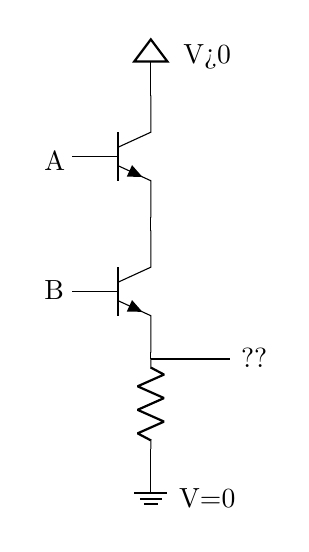
\begin{tikzpicture}
				% Paths, nodes and wires:
				\node[ground] at (1, 4.286){};
				\node[sground, yscale=-1] at (1, 9){};
				\node[shape=rectangle, minimum width=1.197cm, minimum height=0.679cm] at (1.812, 9.429){} node[anchor=north west, align=left, text width=0.809cm, inner sep=6pt] at (1.196, 9.786){V>0};
				\node[shape=rectangle, minimum width=0.608cm, minimum height=0.536cm] at (1.464, 3.857){} node[anchor=north west, align=left, text width=0.22cm, inner sep=6pt] at (1.143, 4.143){V=0};
				\node[npn] at (1, 8.143){};
				\node[npn] at (1, 6.429){};
				\draw (1, 5.571) to[american resistor, /tikz/circuitikz/bipoles/length=1.12cm] (1, 4.429);
				\draw (1, 9) -- (1, 8.913);
				\draw (1, 7.373) -- (1, 7.199);
				\draw (1, 5.659) -- (1, 5.571);
				\draw (1, 4.429) -- (1, 4.286);
				\draw (1, 5.571) -- (2, 5.571);
				\draw (0.16, 6.429) -- (0, 6.429);
				\draw (0.16, 8.143) -- (0, 8.143);
				\node[shape=rectangle, minimum width=0.679cm, minimum height=0.679cm] at (-0.214, 8.071){} node[anchor=north west, align=left, text width=0.291cm, inner sep=6pt] at (-0.571, 8.429){A};
				\node[shape=rectangle, minimum width=0.679cm, minimum height=0.679cm] at (-0.214, 6.429){} node[anchor=north west, align=left, text width=0.291cm, inner sep=6pt] at (-0.571, 6.786){B};
				\node[shape=rectangle, minimum width=0.679cm, minimum height=0.679cm] at (2.286, 5.571){} node[anchor=north west, align=left, text width=0.291cm, inner sep=6pt] at (1.929, 5.929){??};
			\end{tikzpicture}
		\end{column}
	\end{columns}
\end{frame}




\Subsection{Resistors}



\begin{frame}{What is a resistor?}
	light bulb

	ceramic

	the coils in your toaster

	something to soak up energy

	if you run electric current through it and it gets hot, it's a resistor (or at least has resistance)
\end{frame}


\begin{frame}{Voltage Drops in the Resistor}
	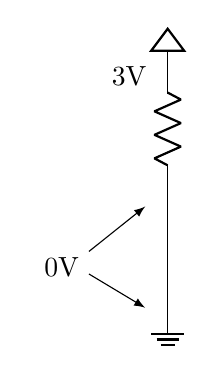
\begin{tikzpicture}
		% Paths, nodes and wires:
		\node[ground] at (2.571, 5.659){};
		\draw (2.571, 8.484) to[american resistor, /tikz/circuitikz/bipoles/length=1.12cm] (2.571, 7.199);
		\node[sground, yscale=-1] at (2.571, 8.484){};
		\node[shape=rectangle, minimum width=0.608cm, minimum height=0.536cm] at (1.964, 8.571){} node[anchor=north west, align=left, text width=0.22cm, inner sep=6pt] at (1.643, 8.857){3V};
		\node[shape=rectangle, minimum width=0.608cm, minimum height=0.536cm] at (1.107, 6.143){} node[anchor=north west, align=left, text width=0.22cm, inner sep=6pt] at (0.786, 6.429){0V};
		\draw[-latex] (1.571, 6.286) -- (2.286, 6.857);
		\draw[-latex] (1.571, 6) -- (2.286, 5.571);
		\draw (2.571, 7.199) -- (2.571, 5.659);
	\end{tikzpicture}
\end{frame}




\begin{frame}{Voltage only drops if it has somewhere to go}

Voltage drop only happens if electricity is flowing. Otherwise the voltage is the same everywhere

	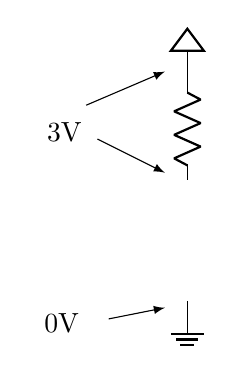
\begin{tikzpicture}
		% Paths, nodes and wires:
		\node[ground] at (2.571, 5.659){};
		\draw (2.571, 8.484) to[american resistor, /tikz/circuitikz/bipoles/length=1.12cm] (2.571, 7.199);
		\node[sground, yscale=-1] at (2.571, 8.484){};
		\node[shape=rectangle, minimum width=0.608cm, minimum height=0.536cm] at (0.893, 7.857){} node[anchor=north west, align=left, text width=0.22cm, inner sep=6pt] at (0.571, 8.143){3V};
		\node[shape=rectangle, minimum width=0.608cm, minimum height=0.536cm] at (0.857, 5.429){} node[anchor=north west, align=left, text width=0.22cm, inner sep=6pt] at (0.536, 5.714){0V};
		\draw[-latex] (1.286, 8.143) -- (2.286, 8.571);
		\draw[-latex] (1.429, 7.714) -- (2.286, 7.286);
		\draw[-latex] (1.571, 5.429) -- (2.286, 5.571);
	\end{tikzpicture}
\end{frame}


\begin{frame}{NOT ALLOWED}
	\begin{columns}
		\begin{column}{0.5\textwidth}
			We assume:
			\begin{itemize}
				\item Top rail fixed at V>0
				\item Bottom rail fixed at 0V
				\item Wires have zero resistance
			\end{itemize}
		\end{column}
		\begin{column}{0.5\textwidth}
			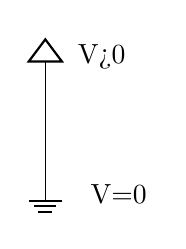
\begin{tikzpicture}
				% Paths, nodes and wires:
				\node[ground] at (1, 8){};
				\node[sground, yscale=-1] at (1, 9){};
				\node[shape=rectangle, minimum width=1.197cm, minimum height=0.679cm] at (1.813, 9.429){} node[anchor=north west, align=left, text width=0.809cm, inner sep=6pt] at (1.196, 9.786){V>0};
				\node[shape=rectangle, minimum width=0.608cm, minimum height=0.536cm] at (1.679, 7.714){} node[anchor=north west, align=left, text width=0.22cm, inner sep=6pt] at (1.357, 8){V=0};
				\draw (1, 9) -- (1, 8);
			\end{tikzpicture}		\end{column}
	\end{columns}

	If you try to build this, one of those assumptions will fail. What might that look like?

\end{frame}


\Subsection{Transistors}

\begin{frame}{Historical Transistors}
	\includegraphics[width=0.5\columnwidth]{images/tube-transistor-wiki}
\end{frame}


\begin{frame}{Modern Transistors}
	\includegraphics[width=\columnwidth]{images/semiconductor-transistor-overkill}
\end{frame}



\begin{frame}{Transistor Behavior}

	https://www.101computing.net/creating-logic-gates-using-transistors/

	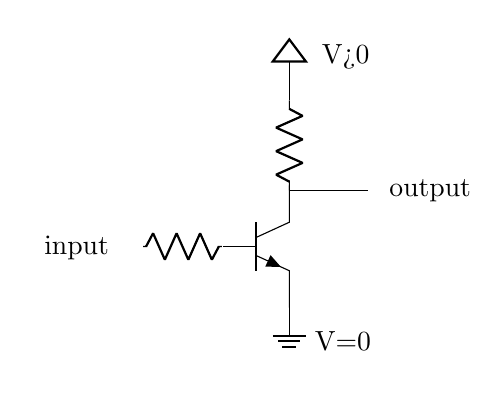
\begin{tikzpicture}
		% Paths, nodes and wires:
		\node[ground] at (1, 6.286){};
		\node[sground, yscale=-1] at (1, 9){};
		\node[shape=rectangle, minimum width=1.197cm, minimum height=0.679cm] at (1.813, 9.429){} node[anchor=north west, align=left, text width=0.809cm, inner sep=6pt] at (1.196, 9.786){V>0};
		\node[shape=rectangle, minimum width=0.608cm, minimum height=0.536cm] at (1.429, 5.857){} node[anchor=north west, align=left, text width=0.22cm, inner sep=6pt] at (1.107, 6.143){V=0};
		\draw (1, 8.857) to[american resistor, /tikz/circuitikz/bipoles/length=1.12cm] (1, 7.714);
		\draw (1, 9) -- (1, 8.857);
		\draw (1, 7.714) -- (2, 7.714);
		\node[shape=rectangle, minimum width=1.197cm, minimum height=0.679cm] at (2.67, 7.714){} node[anchor=north west, align=left, text width=0.809cm, inner sep=6pt] at (2.054, 8.071){output};
		\draw (-0.857, 7) to[american resistor, /tikz/circuitikz/bipoles/length=1.12cm] (0.143, 7);
		\draw (0.286, 7) -- (0.408, 7);
		\node[npn] at (1, 7){};
		\node[shape=rectangle, minimum width=1.197cm, minimum height=0.679cm] at (-1.714, 7){} node[anchor=north west, align=left, text width=0.809cm, inner sep=6pt] at (-2.33, 7.357){input};
	\end{tikzpicture}
\end{frame}


\begin{frame}{Transistor Behavior}
	\begin{columns}
		\begin{column}{0.5\textwidth}
			\usetikzlibrary{shapes.geometric}
			\begin{tikzpicture}
				% Paths, nodes and wires:
				\node[ground] at (1, 6.286){};
				\node[sground, yscale=-1] at (1, 9){};
				\node[shape=rectangle, minimum width=1.197cm, minimum height=0.679cm] at (1.813, 9.429){} node[anchor=north west, align=left, text width=0.809cm, inner sep=6pt] at (1.196, 9.786){V>0};
				\node[shape=rectangle, minimum width=0.608cm, minimum height=0.536cm] at (1.429, 5.857){} node[anchor=north west, align=left, text width=0.22cm, inner sep=6pt] at (1.107, 6.143){V=0};
				\draw (1, 8.857) to[american resistor, /tikz/circuitikz/bipoles/length=1.12cm] (1, 7.714);
				\node[shape=ellipse, draw, line width=1pt, dash pattern={on 1pt off 2pt}, minimum width=1.149cm, minimum height=1.108cm] at (1, 7){};
				\node[shape=rectangle, minimum width=1.197cm, minimum height=0.965cm] at (-1.33, 7.143){} node[anchor=north west, align=left, text width=0.809cm, inner sep=6pt] at (-1.946, 7.643){input\\V>0};
				\draw (1, 6.571) to[cute closed switch] (1, 7.429);
				\draw (1, 9) -- (1, 8.857);
				\draw (1, 7.714) -- (1, 7.429);
				\draw (1, 6.571) -- (1, 6.286);
				\draw (1, 7.714) -- (2, 7.714);
				\node[shape=rectangle, minimum width=1.197cm, minimum height=0.679cm] at (2.67, 7.714){} node[anchor=north west, align=left, text width=0.809cm, inner sep=6pt] at (2.054, 8.071){??};
				\draw (-0.714, 7) to[american resistor, /tikz/circuitikz/bipoles/length=1.12cm] (0.286, 7);
				\draw (0.286, 7) -- (0.408, 7);
			\end{tikzpicture}
		\end{column}
		\begin{column}{0.5\textwidth}
			\usetikzlibrary{shapes.geometric}
			\begin{tikzpicture}
				% Paths, nodes and wires:
				\node[ground] at (1, 6.286){};
				\node[sground, yscale=-1] at (1, 9){};
				\node[shape=rectangle, minimum width=1.197cm, minimum height=0.679cm] at (1.813, 9.429){} node[anchor=north west, align=left, text width=0.809cm, inner sep=6pt] at (1.196, 9.786){V>0};
				\node[shape=rectangle, minimum width=0.608cm, minimum height=0.536cm] at (1.429, 5.857){} node[anchor=north west, align=left, text width=0.22cm, inner sep=6pt] at (1.107, 6.143){V=0};
				\draw (1, 8.857) to[american resistor, /tikz/circuitikz/bipoles/length=1.12cm] (1, 7.714);
				\node[shape=ellipse, draw, line width=1pt, dash pattern={on 1pt off 2pt}, minimum width=1.149cm, minimum height=1.108cm] at (1, 7){};
				\node[shape=rectangle, minimum width=1.197cm, minimum height=0.965cm] at (-1.33, 7.143){} node[anchor=north west, align=left, text width=0.809cm, inner sep=6pt] at (-1.946, 7.643){input\\V=0};
				\draw (1, 6.571) to[cute open switch] (1, 7.429);
				\draw (1, 9) -- (1, 8.857);
				\draw (1, 7.714) -- (1, 7.429);
				\draw (1, 6.571) -- (1, 6.286);
				\draw (1, 7.714) -- (2, 7.714);
				\node[shape=rectangle, minimum width=1.197cm, minimum height=0.679cm] at (2.67, 7.714){} node[anchor=north west, align=left, text width=0.809cm, inner sep=6pt] at (2.054, 8.071){??};
				\draw (-0.714, 7) to[american resistor, /tikz/circuitikz/bipoles/length=1.12cm] (0.286, 7);
				\draw (0.286, 7) -- (0.408, 7);
			\end{tikzpicture}
		\end{column}
	\end{columns}
\end{frame}


\begin{frame}{Transistor Behavior}
	\begin{columns}
		\begin{column}{0.5\textwidth}
			\usetikzlibrary{shapes.geometric}
			\begin{tikzpicture}
				% Paths, nodes and wires:
				\node[ground] at (1, 6.286){};
				\node[sground, yscale=-1] at (1, 9){};
				\node[shape=rectangle, minimum width=1.197cm, minimum height=0.679cm] at (1.813, 9.429){} node[anchor=north west, align=left, text width=0.809cm, inner sep=6pt] at (1.196, 9.786){V>0};
				\node[shape=rectangle, minimum width=0.608cm, minimum height=0.536cm] at (1.429, 5.857){} node[anchor=north west, align=left, text width=0.22cm, inner sep=6pt] at (1.107, 6.143){V=0};
				\draw (1, 8.857) to[american resistor, /tikz/circuitikz/bipoles/length=1.12cm] (1, 7.714);
				\node[shape=ellipse, draw, line width=1pt, dash pattern={on 1pt off 2pt}, minimum width=1.149cm, minimum height=1.108cm] at (1, 7){};
				\node[shape=rectangle, minimum width=1.197cm, minimum height=0.965cm] at (-1.33, 7.143){} node[anchor=north west, align=left, text width=0.809cm, inner sep=6pt] at (-1.946, 7.643){input\\V>0};
				\draw (1, 6.571) to[cute closed switch] (1, 7.429);
				\draw (1, 9) -- (1, 8.857);
				\draw (1, 7.714) -- (1, 7.429);
				\draw (1, 6.571) -- (1, 6.286);
				\draw (1, 7.714) -- (2, 7.714);
				\node[shape=rectangle, minimum width=1.197cm, minimum height=0.679cm] at (2.67, 7.714){} node[anchor=north west, align=left, text width=0.809cm, inner sep=6pt] at (2.054, 8.071){output\\V=0};
				\draw (-0.714, 7) to[american resistor, /tikz/circuitikz/bipoles/length=1.12cm] (0.286, 7);
				\draw (0.286, 7) -- (0.408, 7);
			\end{tikzpicture}
		\end{column}
		\begin{column}{0.5\textwidth}
			\usetikzlibrary{shapes.geometric}
			\begin{tikzpicture}
				% Paths, nodes and wires:
				\node[ground] at (1, 6.286){};
				\node[sground, yscale=-1] at (1, 9){};
				\node[shape=rectangle, minimum width=1.197cm, minimum height=0.679cm] at (1.813, 9.429){} node[anchor=north west, align=left, text width=0.809cm, inner sep=6pt] at (1.196, 9.786){V>0};
				\node[shape=rectangle, minimum width=0.608cm, minimum height=0.536cm] at (1.429, 5.857){} node[anchor=north west, align=left, text width=0.22cm, inner sep=6pt] at (1.107, 6.143){V=0};
				\draw (1, 8.857) to[american resistor, /tikz/circuitikz/bipoles/length=1.12cm] (1, 7.714);
				\node[shape=ellipse, draw, line width=1pt, dash pattern={on 1pt off 2pt}, minimum width=1.149cm, minimum height=1.108cm] at (1, 7){};
				\node[shape=rectangle, minimum width=1.197cm, minimum height=0.965cm] at (-1.33, 7.143){} node[anchor=north west, align=left, text width=0.809cm, inner sep=6pt] at (-1.946, 7.643){input\\V=0};
				\draw (1, 6.571) to[cute open switch] (1, 7.429);
				\draw (1, 9) -- (1, 8.857);
				\draw (1, 7.714) -- (1, 7.429);
				\draw (1, 6.571) -- (1, 6.286);
				\draw (1, 7.714) -- (2, 7.714);
				\node[shape=rectangle, minimum width=1.197cm, minimum height=0.679cm] at (2.67, 7.714){} node[anchor=north west, align=left, text width=0.809cm, inner sep=6pt] at (2.054, 8.071){output\\V>0};
				\draw (-0.714, 7) to[american resistor, /tikz/circuitikz/bipoles/length=1.12cm] (0.286, 7);
				\draw (0.286, 7) -- (0.408, 7);
			\end{tikzpicture}
		\end{column}
	\end{columns}
\end{frame}



\begin{frame}{Why two resistors?}

In many cases, we can get away with just one resistor. The previous example had two. Why?

Always need a resistor between a voltage source and ground. Transistors have internal resistance but it's very small. Easy to burn them out

\end{frame}





\begin{frame}{More Complex Example}
	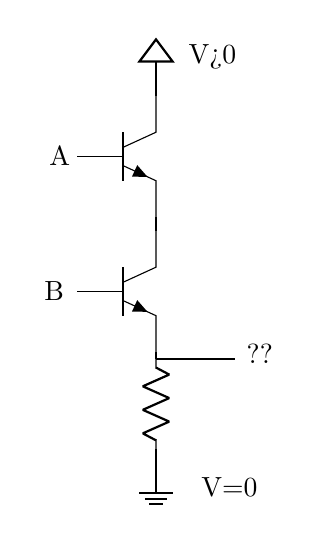
\begin{tikzpicture}
		% Paths, nodes and wires:
		\node[ground] at (1, 4.286){};
		\node[sground, yscale=-1] at (1, 9){};
		\node[shape=rectangle, minimum width=1.197cm, minimum height=0.679cm] at (1.813, 9.429){} node[anchor=north west, align=left, text width=0.809cm, inner sep=6pt] at (1.196, 9.786){V>0};
		\node[shape=rectangle, minimum width=0.608cm, minimum height=0.536cm] at (1.679, 4){} node[anchor=north west, align=left, text width=0.22cm, inner sep=6pt] at (1.357, 4.286){V=0};
		\draw (1, 5.571) to[american resistor, /tikz/circuitikz/bipoles/length=1.12cm] (1, 4.429);
		\node[npn] at (1, 8.143){};
		\node[npn] at (1, 6.429){};
		\draw (1, 9) -- (1, 8.913);
		\draw (1, 7.373) -- (1, 7.199);
		\draw (1, 5.659) -- (1, 5.571);
		\draw (1, 5.571) -- (2, 5.571);
		\draw (0.16, 8.143) -- (0, 8.143);
		\draw (0.16, 6.429) -- (0, 6.429);
		\draw (1, 4.429) -- (1, 4.286);
		\node[shape=rectangle, minimum width=0.668cm, minimum height=0.65cm] at (-0.22, 8.143){} node[anchor=north west, align=left, text width=0.28cm, inner sep=6pt] at (-0.571, 8.485){A};
		\node[shape=rectangle, minimum width=0.668cm, minimum height=0.65cm] at (-0.286, 6.429){} node[anchor=north west, align=left, text width=0.28cm, inner sep=6pt] at (-0.637, 6.771){B};
		\node[shape=rectangle, minimum width=0.668cm, minimum height=0.65cm] at (2.286, 5.628){} node[anchor=north west, align=left, text width=0.28cm, inner sep=6pt] at (1.934, 5.971){??};
	\end{tikzpicture}
\end{frame}




% what is a transistor
% building logic gates

% TEST 3 TOPICS

\Section{Instruction Pipelining}

\Subsection{FDEW Cycle}

\Subsection{Pipelining}

\Subsection{Hazards}

% pipelining
% data hazards
% control hazards

\Section{Assembly Conditionals and Loops}

% b, beq, bne, ...
% if/else
% while loops
% for loops

\input{sections/multiprocessing.tex}
% booting
% forking
% threads, cores, processes
% async


\Section{Appendix}


\Subsection{Raspberry Pi Setup}


\begin{frame}{Pi Setup: Kit Contents}
	\begin{columns}
		\begin{column}{0.5\textwidth}
			\begin{enumerate}
				\item Pi case
				\item Raspberry Pi (in box)
				\item Heat sinks
				\item Power cord
				\item Ethernet to USB adapter
				\item Ethernet cord
				\item USB 2 to USB 3 adapter
				\item SD Card
				\item Accessory case
			\end{enumerate}
		\end{column}
		\begin{column}{0.5\textwidth}
			\includegraphics[width=\columnwidth]{images/pi-kit-contents}
		\end{column}
	\end{columns}
\end{frame}


\begin{frame}{Pi Setup: Apply Heat Sinks}
	\begin{columns}
		\begin{column}{0.5\textwidth}
			\includegraphics[width=\columnwidth]{images/pi-heat-sinks-1}
		\end{column}
		\begin{column}{0.5\textwidth}
			\includegraphics[width=\columnwidth]{images/pi-heat-sinks-2}
		\end{column}
	\end{columns}
\end{frame}

\begin{frame}{Pi Setup: Apply Nonslip Nubs}
	\includegraphics[width=\columnwidth]{images/pi-case-nubs}
\end{frame}

\begin{frame}{Pi Setup: Install in Case}
	\includegraphics[width=\columnwidth]{images/pi-in-case}
\end{frame}

\begin{frame}{Pi Setup: SD Card}
	\begin{columns}
		\begin{column}{0.5\textwidth}
			\includegraphics[width=\columnwidth]{images/pi-sd-card-1}
		\end{column}
		\begin{column}{0.5\textwidth}
			\includegraphics[width=\columnwidth]{images/pi-sd-card-2}
		\end{column}
	\end{columns}
\end{frame}

\begin{frame}{Pi Setup: Connect to Laptop}
	\includegraphics[width=\columnwidth]{images/pi-to-laptop}
\end{frame}

\begin{frame}{Pi Setup: Connect to Power}
\end{frame}

\begin{frame}{Laptop Setup: Enable WiFi}
	\includegraphics[width=\columnwidth]{images/pi-network-settings}
\end{frame}

\begin{frame}{Laptop Setup: Install VSCode}
	\includegraphics[width=\columnwidth]{images/vscode-remote-ssh}
\end{frame}

\begin{frame}{Laptop Setup: Add Remote Connection}
	\includegraphics[width=\columnwidth]{images/vscode-add-remote}
\end{frame}

\begin{frame}{Laptop Setup: SSH Login}
	\begin{itemize}
		\item Default username/password is raspberri/pi
		\item Make sure to update username and password
	\end{itemize}
\end{frame}


\Subsection{CSGit Setup}

% vscode setup
% pi setup
% csgit setup


\end{document}
% positive integers in binary
% arithmetic in binary
% negtive integers
% hex
% fractions
% structured data


\documentclass{beamer}
\usepackage[utf8]{inputenc}
\usepackage[T1]{fontenc}
\usepackage{circuitikz}

\usepackage{multirow}

\title{CS241: Hardware Design}
\date{\today}
\author[Fyfe and Lynn]{Charles Fyfe and Melissa Lynn}
\institute{St Olaf College}

\usetheme{grape}

\usepackage{parskip}
\usepackage{multicol}
\usepackage{graphicx}
% make \oplus look nice
\usepackage{amssymb}

\begin{document}


\titlepage

% just sections up top
\setcounter{tocdepth}{1}

\begin{frame}{Outline}

	\begin{multicols*}{2}
		\tableofcontents
	\end{multicols*}
\end{frame}

% show subsections later
\setcounter{tocdepth}{2}


\Section{Syllabus}

\begin{frame}{Course Overview}

	\includegraphics[width=\columnwidth]{images/dune-robot-hbo}

	{\center
		Thou shalt not make a machine in the likeless of a human mind
	}

	{\small \hfill
		The Orange Catholic Bible, Dune, Frank Herbert
	}
\end{frame}


\begin{frame}{Course Overview}

	Computers feel like magic. You type words. The machine does complex things. Especially in the era of large language models

	But it's not magic. Computers are made of semiconductors, metal, and magnets. Three different kinds of rocks

	This course is about demystifying the machine and exploring how, fundamentally, computers do what they do. Specifically, we'll be looking at:
	\begin{itemize}
		\item The fundamental components of a computer
		\item How data is stored on a computer
		\item Building electrical circuits to perform logic
		\item Programming in Assembly (a very low-level language)
	\end{itemize}
\end{frame}

\Subsection{Grading}

\begin{frame}{Course Grade Breakdown}
	\begin{itemize}
		\item Quizzes and final: 45\%
		\item Homework and labs: 45\%
		\item Participation: 10\%
	\end{itemize}
\end{frame}

\begin{frame}{Standards-Based Grading}
	\begin{itemize}
		\item There are nine standards in the class. Each is worth 5\% of your grade.
		\item There are three quizzes. Each quiz covers three standards.
		\item The final covers all nine standards.
		\item If you demonstrate proficiency on the quiz, you're done with that standard. Full credit. You can skip that part of the final.
		\item If you demonstrate partial proficiency on the quiz, you get half credit. Try again on the final for full credit.
		\item If you do not demonstrate proficiency on the quiz, you get no credit. You can still get full credit on the final!
	\end{itemize}
\end{frame}


\begin{frame}{Homework and Labs}
	\begin{itemize}
		\item One or more lab exercises for each standard. We start these together in class. You may need to finish on your own time.
		\item We will have a homework assignment for each standard.
		\item Please work together in small groups.
		\item Please ensure that the work you turn in reflects your own understanding.
	\end{itemize}
\end{frame}

\begin{frame}{Late Work Policy}
	Please try to get your work in on time.
	\begin{itemize}
		\item If you don't get your work done on time, you may fall behind in the class.
		\item Late work is inconvenient for the TAs. They will be grumpy and vindictive when they grade your work.
		\item TAs will have their own finals to worry about! Late work at the end of the semester might be refused.
	\end{itemize}
	If you need an extension, please reach out beforehand.
\end{frame}

\begin{frame}{Peer Reviews}
	\begin{itemize}
		\item Participation score (10\% of your total grade) is mostly based on peer reviews.
		\item Reviews will be short. Less than one page.
		\item You can get full credit here without too much trouble. Show up. Work together. Make it easy for your peers to say nice things about you.
		\item I recommend keeping notes over the course of the semester when someone is particularly helpful, insightful, etc. Good reviews have concrete examples.
	\end{itemize}
\end{frame}

\Subsection{Office Hours}

\begin{frame}{Office Hours}
	TODO
\end{frame}


\Subsection{Disability Accommodations}

\begin{frame}{Disability Accommodations}
	I am committed to supporting the learning of all students in my class. If you have already
	registered with Disability and Access (DAC) and have your letter of accommodations, please
	meet with me as soon as possible to discuss, plan, and implement your accommodations in the
	course. If you have or think you have a disability (learning, sensory, physical, chronic health,
	mental health or attentional), please contact Disability and Access staff at 507-786-3288 or by visiting \href{https://wp.stolaf.edu/academic-support/dac}{their website}.


	If you have an accommodation that allows you extra time or a low distraction environment for
	quizzes and exams, please email me at least three days before each quiz or exam, so that I can
	make sure to reserve a room.
\end{frame}


\Subsection{Religious Accommodations}

\begin{frame}{Religious Accommodations}
	As part of my commitment to make St Olaf an inclusive community, I will provide students with
	reasonable religious accommodations. If you will be missing class for a religious observance or
	require another religious accommodation, please meet with me to discuss these.
\end{frame}


\Subsection{Academic Integrity}

\begin{frame}{Academic Integrity}

	Plagiarism is a serious academic offense. Hand in your own work. Give credit appropriately when you draw from the work of others. For more information please see:

	\begin{itemize}
		\item \href{https://wp.stolaf.edu/facultyhandbook/academic-integrity-faculty-handbook-category-2}{Faculty Handbook: Academic Integrity}
		\item \href{https://wp.stolaf.edu/honorcouncil/}{The Honor Code}
		\item \href{https://wp.stolaf.edu/roadmap-to-academic-integrity}{Roadmap to Academic Integrity}
	\end{itemize}

	Work that violates this policy will typically receive no credit. In especially serious cases the penalty can be an F in the course.
\end{frame}

\Subsection{AI Use Policy}

\begin{frame}{AI Usage Policy}
	Please not submit AI work as your own.

	You may use AI tools when studying, but be careful. These tools are very good with mainstream languages like Python. We're working with Assembly, which is very much \textbf{not} a mainstream language.

\end{frame}


\Subsection{St Olaf Land Acknowledgement}

\begin{frame}{St Olaf Land Acknowledgement}
	We stand on the homelands of the Wahpekute Band of the Dakota Nation. We honor with
	gratitude the people who have stewarded the land throughout the generations and their ongoing
	contributions to this region. We acknowledge the ongoing injustices that we have committed
	against the Dakota Nation, and we wish to interrupt this legacy, beginning with acts of healing
	and honest storytelling about this place.

	For more information about land acknowledgement statements at St Olaf, please see \href{https://wp.stolaf.edu/education/land-acknowledgement/}{here} and \href{https://wp.stolaf.edu/equity-inclusion/land-acknowledgement/}{here}.
\end{frame}


\Subsection{Statement of Inclusivity}

\begin{frame}{Statement of Inclusivity}
	In keeping with St. Olaf College's mission statement, this class strives to be an inclusive
	learning community, respecting those of differing backgrounds and beliefs. As a community, we
	aim to be respectful to all citizens in this class, regardless of race, ethnicity, religion, gender or
	sexual orientation.
\end{frame}


\Subsection{Gender Pronouns}

\begin{frame}{Gender Pronouns}
	This course affirms people of all gender expressions and gender identities. If you go by a
	different name than what is on the class roster, please let me know.

	Using correct gender
	pronouns is important to me, so you are encouraged to share your pronouns with me and
	correct me if a mistake is made. If you have any questions or concerns, please do not hesitate
	to contact me.
\end{frame}


\Subsection{Multilingual Student Support}

\begin{frame}{Multilingual Student Support}
	I am committed to making course content accessible to all students. If English is not your first
	language and this causes you concern about the course, please speak with me. Students who
	would like extra support with writing or speaking in English can also contact the language support specialist (\href{mailto:berryag@stolaf.edu}{berryag@stolaf.edu}) in the Academic Success Center.
\end{frame}


\Subsection{Mental Health}

\begin{frame}{Mental Health}

	I greatly value your experience in this class, and it is my duty to facilitate a safe, caring, and
	productive learning environment.

	I recognize that you may experience a range of emotional, physical, and/or psychological
	issues, both in and out of the classroom, that may distract you from your learning.

	If you are experiencing such issues, please do not hesitate to come see me. I am here to listen.
	We can also discuss what further resources might be available to you.
\end{frame}

\Subsection{Required Referrals}


\begin{frame}{Required Referrals}
	You are welcome to talk to me about circumstances outside the course that
	affect your classroom experience or acadmic performance. However, please keep
	in mind that I am required to refer cases of discrimination, harassment,
	sexual misconduct, and violence.

	Here are some resources where you can share privately:

	\begin{itemize}
		\item Boe House Counseling Center
		\item College Pastors and Chaplains
		\item Sexual Assault Resource Network (SARN)
		\item Health Services
		\item TimelyCare
	\end{itemize}
\end{frame}




\Subsection{St. Olaf Pride Statement}

\begin{frame}{St. Olaf Pride Statement}
	As an Ole, I will practice:
	\begin{itemize}
		\item Passion for learning and pursuit of vocation
		\item Respect for the worth and dignity of all people
		\item Integrity at all times, in all circumstances
		\item Dedication to a life of service, and
		\item Engagement with my community and the world.
	\end{itemize}
\end{frame}









\Subsection{Important Links}

\begin{frame}{Important Links}
	\begin{itemize}
		\item ARM tutorial https://computerscience.chemeketa.edu/armTutorial/index.html
		\item ARM simulator https://cpulator.01xz.net/?sys=arm
		\item circuit simulator: https://circuitverse.org/simulator
	\end{itemize}
\end{frame}





% TEST 1 TOPICS


\Section{Data Representation}

\begin{frame}{How do computers store information?}
	Computers work using electrical signals which can be on or off. If we let:
	\begin{itemize}
		\item On means 1
		\item Off means 0
	\end{itemize}
	We can use sequences of 0s and 1s to represent information
\end{frame}

\Subsection{Positive Integers in Binary}

\begin{frame}{Numbers in Base Ten (aka Decimal)}
	Let's start by talking about how we write numbers normally.

	For example, let's look at the number 109:
	\begin{align*}
		109 & = 100 \;+\; 0 \;+\; 9                                   \\
		    & = 1 \Times 10^2 \;+\; 0 \Times 10^1 \;+\; 9 \Times 10^0
	\end{align*}
	This way of writing numbers is called base ten.
	We use ten digits (0 to 9 inclusive) and each position in the number is scaled by a power of ten.

	In terms of math, there is nothing special about base ten. We probably use it
	because we have ten fingers. Some ancient civilizations used sompletely
	different systems for counting!
\end{frame}

\begin{frame}{Numbers in Base Two (aka Binary)}
	Computers don't have fingers. They express everything as sequences of 1s and 0s. This format is called binary:

	\begin{align*}
		0b1101101 & =
		1 \Times 2^6 +
		1 \Times 2^5 +
		0 \Times 2^4 +
		1 \Times 2^3 +
		1 \Times 2^2 +
		0 \Times 2^1 +
		1 \Times 2^0                              \\
		          & = 64 + 32 + 0 + 8 + 4 + 0 + 1 \\
		          & = 109                         \\
	\end{align*}
	Importantly: we always use the prefix ``0b'' to avoid confusion when writing numbers in binary.

	1101 is one thousand one hundred and one

	0b1101 is thirteen
\end{frame}

\begin{frame}{Converting from Decimal to Binary}

	If the number is odd, append a 1 on the left. Otherwise, append a 0. Then
	divide your decimal number by two and ignore any remainder. Repeat until your
	decimal number is zero. \\

	For example, starting with 58:

	\begin{itemize}
		\item 58 is even, so append \Highlight{0}. Divide by two, leaving 29.
		\item 29 is odd, so append \Highlight{1}0. Divide by two, leaving 14.
		\item 14 is even, so append \Highlight{0}10. Divide by two, leaving 7.
		\item 7 is odd, so append \Highlight{1}010. Divide by two, leaving 3.
		\item 3 is odd, so append \Highlight{1}1010. Divide by two, leaving 1.
		\item 1 is odd, so append \Highlight{1}11010. Divide by two, leaving 0.
	\end{itemize}

	So 58 in binary is 0b111010.

\end{frame}

\begin{frame}{Converting from Binary to Decimal}

	We can confirm by converting back. The rightmost bit is worth 1, then 2, then
	4, and so on:

	\begin{align*}
		0b111010 & =
		1 \Times 2^5 +
		1 \Times 2^4 +
		1 \Times 2^3 +
		0 \Times 2^2 +
		1 \Times 2^1 +
		0 \Times 2^0                          \\
		         & = 32 + 16  + 8 + 0 + 2 + 0 \\
		         & = 58
	\end{align*}

\end{frame}

\begin{frame}{Addition in Binary}
	Binary addition works just like decimal addition.
	Start from the right, add straight down, and carry when you run out of digits.

	For example:
	\[
		\begin{array}{ccccccccc}
			1 & 1 & 1 & 1 & 1 &   &   &   &   \\
			  & 0 & 0 & 1 & 1 & 1 & 0 & 0 & 0 \\
			+ & 1 & 1 & 1 & 0 & 1 & 0 & 0 & 1 \\
			\hline
			1 & 0 & 0 & 1 & 0 & 0 & 0 & 0 & 1 \\
		\end{array}
	\]

	What happens if we try to perform this operation but we only have 8 bits to
	store the answer?
\end{frame}

\begin{frame}{Multiplication in Binary}
	Binary multiplication works just like decimal multiplication.
	Multiply the top number by the rightmost digit of the bottom number.
	Then move to the next line, add a zero, and repeat for the next digit.
	Finally, add up the lines. For example:
	\[
		\begin{array}{cccccc}
			  &   &        & 1 & 1 & 0 \\
			  &   & \times & 1 & 0 & 1 \\
			\hline
			  &   &        & 1 & 1 & 0 \\
			  &   & 0      & 0 & 0 & 0 \\
			+ & 1 & 1      & 0 & 0 & 0 \\
			\hline
			  & 1 & 1      & 1 & 1 & 0 \\
		\end{array}
	\]
\end{frame}

\begin{frame}{Division in Binary}
	To divide by 2, shift the bits one place to the right. \\

	To divide by 4, shift the bits two places to the right. \\

	That's about as deep as we go in this class. If you're curious to learn more,
	see the textbook.

\end{frame}



\Subsection{Hexadecimal}

\begin{frame}{What? Why?}

	Binary is how machines store data. But writing out binary by hand is a chore.
	In practice, it's often convenient to use hexadecimal (base 16) instead.

	\begin{itemize}
		\item Decimal uses ten digits, 0-9
		\item Binary uses two digits, 0 and 1
		\item Hexadecimal uses sixteen digits: 0-9 along with A-F
	\end{itemize}
	Hexadecimal values are always prefixed with ``0x'' to avoid ambiguity.
\end{frame}

\begin{frame}{Converting Between Binary and Hexadecimal}

	Converting back and forth between binary and hexadecimal does not require any
	math! Every four bits become one hex digit.
	\begin{align*}
		0b0000 & = 0x0 = 0 & 0b1000 & = 0x8 = 8  \\
		0b0001 & = 0x1 = 1 & 0b1001 & = 0x9 = 9  \\
		0b0010 & = 0x2 = 2 & 0b1010 & = 0xA = 10 \\
		0b0011 & = 0x3 = 3 & 0b1011 & = 0xB = 11 \\
		0b0100 & = 0x4 = 4 & 0b1100 & = 0xC = 12 \\
		0b0101 & = 0x5 = 5 & 0b1101 & = 0xD = 13 \\
		0b0110 & = 0x6 = 6 & 0b1110 & = 0xE = 14 \\
		0b0111 & = 0x7 = 7 & 0b1111 & = 0xF = 15 \\
	\end{align*}
\end{frame}

\begin{frame}{Converting Hexadecimal to Decimal}

	Hexadecimal is base 16. So each place corresponds to a power of 16.

	\begin{align*}
		0x3AB & = 3 \times 16^2 + 10 \times 16^1 + 11 \times 16^0 \\
		      & = 3 \times 256 + 10 \times 16 + 11 \times 1       \\
		      & = 768 + 160 + 11                                  \\
		      & = 954                                             \\
	\end{align*}

	Hexadecimal is very compact! These numbers get big fast

\end{frame}

\begin{frame}{Arithmetic in Hexadecimal}

	Addition and multiplication work in hexadecimal just like they do in binary and
	decimal. Just be careful about carrying.

	\[
		\begin{array}{ccccc}
			1 &   &   & 1 &   \\
			  & 4 & 1 & 7 & B \\
			+ & C & 2 & 0 & F \\
			\hline
			1 & 0 & 3 & 8 & A \\
		\end{array}
	\]

\end{frame}






\Subsection{Negatives in Binary}

\begin{frame}{First Attempt: Signed Magnitude}

	We can use the first digit to hold the sign, then the rest of the digits to
	hold magnitue:

	\begin{itemize}
		\item 0b\Highlight{0}1011001 is positive 10110001, so 89
		\item 0b\Highlight{1}1011001 is negative 1011001, so -89
	\end{itemize}

	This is nice and straightforward!

\end{frame}

\begin{frame}{Addition and Subtraction with Signed Magnitude}
	Adding positive numbers works just the same. But what happens if we throw a minus sign in there?

	For example, let's look at 12 - 5. First, rewrite it as 12 + (-5). Then:

	\[
		\begin{array}{ccccccccc}
			  & 0 & 0 & 0 & 0 & 1 & 1 & 0 & 0 \\
			+ & 1 & 0 & 0 & 0 & 0 & 1 & 0 & 1 \\
			\hline
			  & ? & ? & ? & ? & ? & ? & ? & ? \\
		\end{array}
	\]

	We know the result should be 7 (0b00000111). But our regular rules for addition
	do not get us there.
\end{frame}

\begin{frame}{Zero with Signed Magnitude}

	Using signed magnitude, 0b00000000 is zero.

	And 0b10000000 is negative zero (which is also zero).

	Using this convention, we have to worry about the difference between numerical
	equality and bitwise equality. That seems pretty messy.
\end{frame}

\begin{frame}{Can We Do Better?}
	Signed magnitude was a swing and a miss. What do we want when we talk about negative numbers?
	\begin{itemize}
		\item We want positive numbers to work like we expect
		\item We want 0b00000000 to be zero, with no ambiguity
		\item We want addition and subtraction to work the same for positive and negative
	\end{itemize}
\end{frame}

\begin{frame}{Another Idea: Two's Complement}
	We know 1 - 1 = 0. Put another way, 1 + (-1) = 0. Can we work backwards from there to figure out how to write -1?
	\[
		\begin{array}{ccccccccc}
			  & 0 & 0 & 0 & 0 & 0 & 0 & 0 & 1 \\
			+ & 1 & 1 & 1 & 1 & 1 & 1 & 1 & 1 \\
			\hline
			  & 0 & 0 & 0 & 0 & 0 & 0 & 0 & 0 \\
		\end{array}
	\]

	Remember: on a computer, our numbers have to fit in a set number of bits.
	Anything past that gets thrown away. This is called overflow. In this case,
	overflow works in our favor!
\end{frame}

\begin{frame}{Working Backwards from Zero}
	We can use the same trick to identify the rest of the negative numbers:
	\begin{itemize}
		\item 0b00000000 is 0
		\item 0b11111111 is -1
		\item 0b11111110 is -2
		\item 0b11111101 is -3
		\item 0b11111100 is -4
		\item etc
	\end{itemize}

\end{frame}

\begin{frame}{The Sign Bit (Again)}
	We only have 256 possible integers. How do we decide where the positives end and the negatives begin?

	Unsigned int: bits are worth 1, 2, 4, 8, 16, 32, 64, 128

	Signed magnitude: bits are worth $\pm1, \pm2, \pm4, \pm8, \pm16, \pm32, \pm64$,
	and the last bit tells us whether to use positive or negative (yikes)

	Two's complement: bits are worth 1, 2, 4, 8, 16, 32, 64, \Highlight{-128}

	Range of possible values is -128 to 127.
\end{frame}

\begin{frame}{Flipping Signs in Two's Complement}
	To flip the sign of a two's complement integer, flip all the bits then add 1. Ignore the overflow (if any). This works for both positive and negative numbers.

	For example:
	\begin{itemize}
		\item 55 is 0b01010111
		\item Flip the bits: 0b10101000, then add 1: 0b10101001
		\item So -55 is 0b10101001
		\item Flip the bits again: 0b01010110, add 1: 0b01010111
		\item So -(-55) = 55 = 0b01010111
	\end{itemize}

	What happens if we negate zero?
\end{frame}

\begin{frame}{Overflow}
	Overflow is important for two's complement. It ensures that positive zero and negative zero are the same. But it is also a constraint!

	Try adding 0b01101001 + 0b01011010:
	\[
		\begin{array}{ccccccccc}
			  &   & 1 & 1 & 1 &   &   &   &   \\
			  & 0 & 1 & 1 & 0 & 1 & 0 & 0 & 1 \\
			+ & 0 & 1 & 0 & 1 & 1 & 0 & 1 & 0 \\
			\hline
			  & 1 & 1 & 0 & 0 & 0 & 0 & 1 & 1 \\
		\end{array}
	\]

	These are two's complement numbers. Convert them to decimal. What just
	happened?

\end{frame}


\Subsection{Fractions and Decimals}

\begin{frame}{The Decimal Point}

	Sometimes we need to store numbers that aren't integers. \\

	Before we worry about binary, what does 21.867 mean? \\

	\begin{align*}
		21.867 & = 2 \Times 10^1 + 1 \Times 10^0 + 8 \Times ?? + 6 \Times ?? + 7 \Times ??
	\end{align*}

\end{frame}

\begin{frame}{The Decimal Point}

	In decimal:
	\begin{align*}
		21.867 & = 2 \Times 10^1 + 1 \Times 10^0 + 8 \Times 10^{-1} + 6 \Times 10^{-2} + 7 \Times 10^{-3}             \\
		       & =2 \Times 10 + 1 \Times 1 + 8 \Times \frac{1}{10} + 6 \Times \frac{1}{100} + 7 \Times \frac{1}{1000} \\
	\end{align*}

	In binary, we can use the same idea:
	\begin{align*}
		0b101.010 & = 1 \Times 2^2 + 0 \Times 2^1 + 1 \Times 2^0 + 0 \Times 2^{-1} + 1 \Times 2^{-2} + 0 \Times 2^{-3} \\
		          & = 1 \Times 4 + 0 + 1 \Times 1 + 0 + 1 \Times \frac{1}{4} + 0                                       \\
		          & = 5.25                                                                                             \\
	\end{align*}

\end{frame}

\begin{frame}{Fixed Point Representation}

	The computer just stores 1s and 0s, not decimal points. How do we distinguish
	these values?
	\begin{itemize}
		\item 0b0101110.1 = 46.5
		\item 0b010111.01 = 23.25
		\item 0b01011.101 = 11.625
	\end{itemize}

	One option is to specify the location of the decimal point ahead of time. For
	example, we could say that our eight-bit binary decimal always has two decimal
	bits. \\

	What is an upside of this approach? What is a downside?

\end{frame}

\begin{frame}{Floating Point Representation}

	Floating point numbers are a bit more complicated, but much more flexible. For
	a 16-bit floating point number we get:

	\begin{itemize}
		\item 1 bit for the sign
		\item 5 bits for the exponent (value -14 to 15)
		\item 10 bits for the significand (value 0 to 1023)
	\end{itemize}

	To turn those components into a value we use:
	\begin{align*}
		\text{value} & = (-1)^{\text{sign}} \times 2^{\text{exponent} - 15} \times \left(1 + \frac{\text{significand}}{1024} \right)
	\end{align*}

	Why offset the exponent?

	Why add 1 to the significand fraction?

\end{frame}

% Explanation here for the 127 offset: https://www.quora.com/Why-do-we-add-127-to-the-exponent-in-IEEE-754-floating-number-format-to-get-the-actual-exponent-value

\begin{frame}{Floating Point Examples}

	\begin{align*}
		\underbrace{0}_\text{sign} \; \underbrace{01111}_\text{exponent} \; \underbrace{0000000000}_\text{significand} & = (-1)^0 \times 2^{15 - 15} \times \left( 1 + \frac{0}{1024} \right) \\
		                                                                                                               & = 1 \times 2^0   \times \left( 1 + 0 \right)                         \\
		                                                                                                               & = 1                                                                  \\
	\end{align*}
	\begin{align*}
		0 \; 01101 \; 0101010101 & = (-1)^0 \times 2^{13 - 15} \times \left( 1 + \frac{341}{1024} \right) \\
		                         & \approx 0.33325195                                                     \\
	\end{align*}
	\begin{align*}
		1 \; 11110 \; 1111111111 & = (-1)^1 \times 2^{30 - 15} \times \left( 1 + \frac{1023}{1024} \right) \\
		                         & = -65504                                                                \\
	\end{align*}

	Why
\end{frame}

\begin{frame}{Floating Point Special Cases}

	\[
		\begin{array}{ccccr}
			0 & 00000 & 0000000000     & = 0          \\
			1 & 00000 & 0000000000     & = -0         \\
			0 & 11111 & 0000000000     & = \infty     \\
			1 & 11111 & 0000000000     & = -\infty    \\
			0 & 11111 & \text{nonzero} & = \text{NaN} \\
		\end{array}
	\]

	There's more to it than this. If you're curious, read up on subnormal numbers
	\href{https://en.wikipedia.org/wiki/Half-precision_floating-point_format}{here}

\end{frame}

\begin{frame}{Floating Point for Big Integers}

	If we're dealing with big numbers, floating point often works better than fixed
	point. This is true even if both formats use the same number of bits.

	\begin{itemize}
		\item 8-bit unsigned integer: max value 255
		\item 16-bit unsigned integer: max value 65,535
		\item 32-bit unsigned integer: max value 4.2 billion % 4,294,967,295
		\item 16-bit floating point: max value 65,504 (also handles negatives, fractions)
		\item 32-bit floating point: max value 340 billion billion billion billion (also handles negatives, fractions)
		      % 340,282,346,638,528,859,811,704,183,484,516,925,440 
	\end{itemize}

\end{frame}

\begin{frame}{Floating Point Limitations}

	So what's the catch?

\end{frame}

%        \item Convert 0b100110.10 from fixed-point binary to decimal.
%        \item Convert 23.75 from decimal to fixed-point binary.
%        \item Add fixed-point binary numbers 0b101101.01 + 0b010011.11. Convert to decimal to confirm your result.
%        \item Show that the 16-bit floating point expression ${1 \; 01000 \; 1100000000}$ is equal to -3.5 in decimal.

\Subsection{Beyond Numbers}

\begin{frame}{What else do computers store?}
	There are many cases where we want a computer to store non-numerical data:
	\begin{itemize}
		\item Text
		\item Colors
		\item Sounds
		\item Images
		\item Videos
		\item Websites
		\item Multiple things at once
	\end{itemize}
\end{frame}

\begin{frame}{Characters and Strings}
	\begin{itemize}
		\item Each character is represented by a number
		\item The most straightforward encoding is ASCII
		\item Modern use cases typically use Unicode (much bigger)
		\item To make a string, put a bunch of characters in a row
		\item Question: how do we identify the end of a string?
	\end{itemize}
\end{frame}

\begin{frame}{ASCII Table}
	\includegraphics[width=\columnwidth]{images/ascii-table}
\end{frame}

\begin{frame}{Colors and Images}
	\begin{itemize}
		\item A color can be described by three numbers (R, G, B)
		\item We can represent an image as a grid of colored pixels
		\item Question: do we need a null byte at the end of a pixel/row/image? Why or why not?
	\end{itemize}
	\includegraphics[width=\columnwidth]{images/mario-pixels}
\end{frame}

\begin{frame}{Sound}
	\begin{itemize}
		\item Sound is pressure vibrations in the air
		\item We can create sound by moving a speaker cone rapidly
		\item To store sound, store the movement of the speaker cone
	\end{itemize}
	\includegraphics[width=0.5\columnwidth]{images/speakers}
\end{frame}

\begin{frame}{Structured Data}
	\begin{itemize}
		\item When you go to a website, how does your browser know what to display?
		\item When you add an item to your online cart, what data is sent?
	\end{itemize}
	\begin{columns}
		\begin{column}{0.5\textwidth}
			\includegraphics[width=\columnwidth]{images/html-example}
		\end{column}
		\begin{column}{0.5\textwidth}
			\includegraphics[width=\columnwidth]{images/json-example}
		\end{column}
	\end{columns}
\end{frame}









% positive integers in binary
% arithmetic in binary
% negtive integers
% hex
% fractions
% structured data

\input{sections/02-boolean-logic.tex}
% boolean operators
% boolean expressions
% boolean circuits

\Section{Assembly Globals}

\begin{frame}{Coding in Assembly}

	You'll be doing coding exercises on an online emulator, as well as on your Raspberry Pi

\end{frame}

\Subsection{Why study assembly?}

\begin{frame}[fragile]{Hello World in C}
	\begin{minted}{C}
		#include <stdio.h>

		int main() {
			printf("Hello world!\n");
			return 0;
		}
	\end{minted}

	Your local C compiler can turn this into an executable, which you can then run:

	\begin{minted}{bash}
		$ gcc hello.c
		$ ./a.out
		Hello world!
	\end{minted}
\end{frame}


\begin{frame}[fragile]{Hello World in Python}
	\begin{minted}{python}
		print('Hello world!')
	\end{minted}

	You can run this using your local Python interpreter:
	\begin{minted}{bash}
		$ python3 hello.py
		Hello world!
	\end{minted}
\end{frame}

\begin{frame}[fragile]{Hello World in Assembly}
	% haven't yet found a perfect highlighter match
	% tasm - dislikes pound signs for int literals
	% nasm, gas - dislikes comments with @
	% ca65 - comments and a lot of commands all black
	% llvm, dasm16, hsail - nope
	% hsail
	\begin{minted}{tasm}
		.section .rodata
		greeting: .ascii "Hello world!\n\0"

		.section .text
		.global _start
		_start:
		ldr r0, =greeting
		bl printf
		mov r0, #0
		bl exit
	\end{minted}

	You can assemble this into an executable and run it on your Raspberry Pi:
	\begin{minted}{bash}
		$ gcc hello.s
		$ ./a.out
		Hello world!
	\end{minted}
\end{frame}

\begin{frame}{What makes assembly special?}
	\begin{itemize}
		\item It takes a lot of lines to do anything
		\item There is so much boilerplates
		\item Yikes
	\end{itemize}
\end{frame}

\begin{frame}{What makes assembly special?}
	\begin{itemize}
		\item Every computer architecture is a little bit different. An Intel CPU and an AMD CPU can both run the same logic, but they will do things in slightly different ways.
		\item When coding in C, you (mostly) don't have to worry about it. The compiler figures out how to make your logic work on the current hardware.
		\item Same for Python. The interpreter (written in C and compiled) figures out how to make your logic work on the current hardware.
		\item Assembly is not like that. Intel assembly is tied to the hardware specifics of the Intel CPU. ARM assembly is a different language.
		\item We study assembly because we want to talk about what is happening on hardware.
	\end{itemize}

	%	The following command compiles a program in C:
	%	\begin{minted}{bash}
	%		gcc hello.c -o hello
	%	\end{minted}
	%	This creates several intermediate files, eventually creating an executable file (which we can run).
	%	`hello.c' -> preprocessor -> `hello.i' -> compiler -> `hello.s' -> assembler -> `hello.o' -> linker -> `hello'

\end{frame}

% per wikipedia:
% Each computer architecture has its own machine language. Computers differ in the number and type of operations they support, in the different sizes and numbers of registers, and in the representations of data in storage. While most general-purpose computers are able to carry out essentially the same functionality, the ways they do so differ; the corresponding assembly languages reflect these differences.

\Subsection{Global Constants}

\begin{frame}{Global Constants}
	\begin{itemize}
		\item A global constant is defined in the code
		\item Its value does not change during runtime
		\item It has a name
		\item We can use the name to load the \textbf{address} of that value
	\end{itemize}
\end{frame}

\Subsection{Printf}


\begin{frame}[fragile]{Favorite Number}
	\begin{minted}{tasm}
		.section .rodata
		output_str: .ascii "My favorite number is %d\n\0"
		favorite_num: .word 123
		
		.section .text
		.global main
		main:
		ldr r0, =output_str
		ldr r1, =favorite_num
		ldr r1, [r1]
		bl printf
		mov r0, #0
		b exit
	\end{minted}
\end{frame}











\Subsection{Global Variables}

\Subsection{Scanf}






\begin{frame}{Registers and Memory}
	\includegraphics[width=0.7\columnwidth]{images/pi-part-labels}
\end{frame}

\begin{frame}{Registers and Memory}
	\begin{itemize}
		\item The \emph{CPU} is where computations actually happen.
		\item The CPU includes tiny bits of storage for the values it's using right now. These are called \emph{registers}.
		\item All other data is stored in \emph{memory} (aka RAM). This includes data as well as the program instructions themselves.
		\item When coding in C or Python, you do not need to worry about registers. You declare variables and the computer figures it out.
		\item When coding in Assembly, we manually move data back and forth between memory and registers.
	\end{itemize}
\end{frame}

\begin{frame}{Registers and Memory}
	Memory stores data and program instructions
	CPU does the work
	Registers are tiny tiny bits of storage right next to the CPU

	Memory is your bookshelf
	Desk is registers
	You are the CPU
	If you want to read or write anything, you have to take the book from your shelf and put it on the desk.


	In C and Python, you don't worry about registers. You declare variables in memory and the compiler figures out how and when to do appropriate reads and writes
	In Assembly, you have to manually shuffle values back and forth between memory and the registers

\end{frame}



\begin{frame}[fragile]{Hello World in Assembly (again)}
	\begin{minted}{tasm}
		.section .rodata
		greeting: .ascii "Hello world!\n\0"

		.section .text
		.global _start
		_start:
		ldr r0, =greeting
		bl printf
		mov r0, #0
		bl exit
	\end{minted}

	Let's walk through what's happening on each line
\end{frame}





\begin{frame}[fragile]{Hello World in Assembly}
	\begin{alltt}
		\Highlight{@ global read-only data (aka constants)}
		.section .rodata
		greeting: .ascii "Hello World!{\textbackslash}n{\textbackslash}0"

		\Highlight{@ execution starts here}
		.section .text
		.global main
		main:
		\Highlight{@ load the string address to r0}
		ldr r0, =greeting
		\Highlight{@ print the string from r0}
		bl printf
		\Highlight{@ return 0 (normal exit status)}
		mov r0, \#0
		bl exit
	\end{alltt}
\end{frame}



\begin{frame}{Hello World in Assembly}

	{\Huge
		TODO: don't worry about PC yet? they haven't done the von neumann arch section yet}

\end{frame}



\begin{frame}{Hello World with Instruction Addresses}
	\begin{alltt}
		\begin{tabular}{ r | l }
			-      & \Highlight{@ global read-only data (aka constants)}               \\
			-      & .section .rodata                                                  \\
			-      & greeting: .ascii "Hello World!{\textbackslash}n{\textbackslash}0" \\
			-      & \Highlight{@ execution starts here}                               \\
			-      & .section .text                                                    \\
			-      & .global main                                                      \\
			-      & main:                                                             \\
			-      & \quad \Highlight{@ load the string address to r0}                 \\
			0x4fe0 & \quad ldr r0, =greeting                                           \\
			-      & \quad \Highlight{@ print the string from r0}                      \\
			0x4fe4 & \quad bl printf                                                   \\
			-      & \quad \Highlight{@ return 0 (normal exit status)}                 \\
			0x4fe8 & \quad mov r0, \#0                                                 \\
			0x4fec & \quad bl exit                                                     \\
		\end{tabular}
	\end{alltt}
\end{frame}

\begin{frame}{Hello World Walkthrough (0)}
	\begin{alltt}
		\begin{tabular}{ r | l p{5mm} r | l }
			\multicolumn{2}{c}{Registers} &        & \multicolumn{2}{c}{Memory}                              \\
			r0                            & ?      &                            & 0x4fe0 & ldr r0, =greeting \\
			r1                            & ?      &                            & 0x4fe4 & bl printf         \\
			r2                            & ?      &                            & 0x4fe8 & mov r0, \#0       \\
			r3                            & ?      &                            & 0x4fec & bl exit           \\
			r4                            & ?      &                            & 0x4ff0 & Hell              \\
			sp                            & ?      &                            & 0x4ff4 & o Wo              \\
			fp                            & ?      &                            & 0x4ff8 & rld!              \\
			pc                            & 0x4fe0 &                            & 0x4ffc & {\textbackslash}0 \\
			lr                            & ?      &                            & 0x5000 & ?                 \\
		\end{tabular}
	\end{alltt}

	The operating system loads instructions and global constants into memory. The program counter \texttt{pc} points to the start of execution.

\end{frame}

\begin{frame}{Hello World Walkthrough (1)}
	\begin{alltt}
		\begin{tabular}{ r | l p{5mm} r | l }
			\multicolumn{2}{c}{Registers} &        & \multicolumn{2}{c}{Memory}                              \\
			r0                            & 0x4ff0 &                            & 0x4fe0 & ldr r0, =greeting \\
			r1                            & ?      &                            & 0x4fe4 & bl printf         \\
			r2                            & ?      &                            & 0x4fe8 & mov r0, \#0       \\
			r3                            & ?      &                            & 0x4fec & bl exit           \\
			r4                            & ?      &                            & 0x4ff0 & Hell              \\
			sp                            & ?      &                            & 0x4ff4 & o Wo              \\
			fp                            & ?      &                            & 0x4ff8 & rld!              \\
			pc                            & 0x4fe4 &                            & 0x4ffc & {\textbackslash}0 \\
			lr                            & ?      &                            & 0x5000 & ?                 \\
		\end{tabular}
	\end{alltt}

	Use \texttt{ldr} to load the address of global constant \texttt{greeting} to \texttt{r0}

	Also increment \texttt{pc} to point to the next instruction

\end{frame}

\begin{frame}{Hello World Walkthrough (2)}
	\begin{alltt}
		\begin{tabular}{ r | l p{5mm} r | l }
			\multicolumn{2}{c}{Registers} &        & \multicolumn{2}{c}{Memory}                              \\
			r0                            & 0x4ff0 &                            & 0x4fe0 & ldr r0, =greeting \\
			r1                            & ?      &                            & 0x4fe4 & bl printf         \\
			r2                            & ?      &                            & 0x4fe8 & mov r0, \#0       \\
			r3                            & ?      &                            & 0x4fec & bl exit           \\
			r4                            & ?      &                            & 0x4ff0 & Hell              \\
			sp                            & ?      &                            & 0x4ff4 & o Wo              \\
			fp                            & ?      &                            & 0x4ff8 & rld!              \\
			pc                            & 0x4fe8 &                            & 0x4ffc & {\textbackslash}0 \\
			lr                            & ?      &                            & 0x5000 & ?                 \\
		\end{tabular}
	\end{alltt}

	Use \texttt{bl} to call the built-in function \texttt{printf}, which looks at the address from \texttt{r0} and prints the data as a null-terminated string

	Also increment \texttt{pc} to point to the next instruction


\end{frame}

\begin{frame}{Hello World Walkthrough (3)}
	\begin{alltt}
		\begin{tabular}{ r | l p{5mm} r | l }
			\multicolumn{2}{c}{Registers} &        & \multicolumn{2}{c}{Memory}                              \\
			r0                            & 0      &                            & 0x4fe0 & ldr r0, =greeting \\
			r1                            & ?      &                            & 0x4fe4 & bl printf         \\
			r2                            & ?      &                            & 0x4fe8 & mov r0, \#0       \\
			r3                            & ?      &                            & 0x4fec & bl exit           \\
			r4                            & ?      &                            & 0x4ff0 & Hell              \\
			sp                            & ?      &                            & 0x4ff4 & o Wo              \\
			fp                            & ?      &                            & 0x4ff8 & rld!              \\
			pc                            & 0x4fec &                            & 0x4ffc & {\textbackslash}0 \\
			lr                            & ?      &                            & 0x5000 & ?                 \\
		\end{tabular}
	\end{alltt}

	Move the value zero to \texttt{r0}

	Also increment \texttt{pc} to point to the next instruction


\end{frame}

\begin{frame}{Hello World Walkthrough (4)}
	\begin{alltt}
		\begin{tabular}{ r | l p{5mm} r | l }
			\multicolumn{2}{c}{Registers} &   & \multicolumn{2}{c}{Memory}                              \\
			r0                            & 0 &                            & 0x4fe0 & ldr r0, =greeting \\
			r1                            & ? &                            & 0x4fe4 & bl printf         \\
			r2                            & ? &                            & 0x4fe8 & mov r0, \#0       \\
			r3                            & ? &                            & 0x4fec & bl exit           \\
			r4                            & ? &                            & 0x4ff0 & Hell              \\
			sp                            & ? &                            & 0x4ff4 & o Wo              \\
			fp                            & ? &                            & 0x4ff8 & rld!              \\
			pc                            & ? &                            & 0x4ffc & {\textbackslash}0 \\
			lr                            & ? &                            & 0x5000 & ?                 \\
		\end{tabular}
	\end{alltt}

	Use \texttt{bl} to call the built-in \texttt{exit} function, which exits from the program. The value in \texttt{r0} is the returncode.

	The value of \texttt{pc} is restored for the upstream caller (we'll worry more about this in later chapters)

\end{frame}




\Subsection{Assembly Commands}

\begin{frame}{commands in assembly}

	leave local variable handling for later. str, ldr with brackets

	\begin{itemize}
		\item add rd, rn, \# ... add rd, rn1, rn2
		\item sub rd, rn, \# ... sub rd, rn1, rn2
		\item mov rd, rn ... mov rd, \#
		\item mul rd, rn1, rn2
		\item ldr rd, =label
		\item ldr, rd, [rn]
		\item ldr, rd, [rn, \#]
		\item str rs, rn
	\end{itemize}

\end{frame}




\Subsection{Memory Diagrams}


\Subsection{Automated Testing}







% why study assembly?
% global variables
% mov
% printf
% ldr
% scanf
% add, mul

% TEST 2 TOPICS

\input{sections/04-instructions-on-hardware.tex}
% parts of a computer
% executing instructions
% the von neumann bottleneck
% memory hierarchy
% block-driven execution
% instruction walkthrough

\Section{Assembly Functions}


\Subsection{The Stack}

\begin{frame}{Push and Pop}

	When a program starts running, the OS loads the instructions into memory.

	It also allocates memory for the program to use during execution

	There is a special register called the stack pointer which provides the location of that memory

\end{frame}


\begin{frame}{Working Memory}
	\begin{columns}
		\begin{column}{0.5\textwidth}

			we do not know what piece of memory the OS will provide

			arbitrarily say it starts at 0x5000

			stack pointer points to the "bottom" of our available memory. we work our way "up" by subtracting from the stack pointer

			The rules are the same when we call a function. It looks at SP to know the "bottom" of its available memory, then works up from there

		\end{column}
		\begin{column}{0.5\textwidth}
			\begin{alltt}
				\begin{tabular}{ r | l }
					0x4ff8 & \vdots           \\
					0x4ffc & available        \\
					0x5000 & available        \\
					0x5004 & in use by parent \\
					0x5008 & in use by parent \\
					0x500c & \vdots           \\
				\end{tabular}
			\end{alltt}
		\end{column}
	\end{columns}

\end{frame}


\Subsection{Calling a Function}


\begin{frame}{Branch and Link}

	New command: BL

	Branch and Link

	Branch = modify PC. Recall: PC tells us what to do next. Usually we just do the next line. In this case, we will jump to some other part of the program. This is how we call a function.

	Link = set LR to the PC of the next line. Once we're done with the function, this is how we return to the parent context.

\end{frame}

\Subsection{Stack Frames}


\begin{frame}{Frame Pointer}

	\begin{itemize}
		\item Not strictly necessary
		\item Code is easier to read
		\item Integration with debugging tools
		\item Stack pointer can move during the function
		\item Skipping the frame pointer can be skipped by some compilers
	\end{itemize}

	% https://stackoverflow.com/questions/46797915/what-are-the-advantages-of-a-frame-pointer

\end{frame}


\begin{frame}{SIMD}

	\begin{itemize}
		\item SIMD - single instruction, multiple data
		\item 64 bit architecture (8 bytes)
		\item there are cases where it works in chunks of 16 bytes
		\item I don't have time to worry about that, and neither do you. For the purposes of this class, everything is 16 bytes.
		\item This is wasteful! We are using double the memory we need, sometimes more
		\item That's ok. We are not trying to become assembly developers. We are getting exposure to important concepts
	\end{itemize}

\end{frame}



\begin{frame}{Stack Frame Walkthrough}
	\small
	\begin{columns}
		\begin{column}{0.5\textwidth}
			\begin{alltt}
				\begin{tabular}{r | l}
					       & {\quad}.section .rodata \\
					       &                         \\
					       & {\quad}.text            \\
					       & func:                   \\
					0x3fd4 & {\quad}push \{fp, lr\}  \\
					0x3fd8 & {\quad}add fp, sp, \#4  \\
					0x3fdc & {\quad}sub sp, sp, \#4  \\
					0x3fe0 & {\quad}@ ...            \\
					0x3fe4 & {\quad}sub sp, fp, \#4  \\
					0x3fe8 & {\quad}pop \{fp, pc\}   \\
					       &                         \\
					       & {\quad}.global main     \\
					       & main:                   \\
					0x3fec & {\quad}push \{fp, lr\}  \\
					0x3ff0 & {\quad}add fp, sp, \#4  \\
					0x3ff4 & {\quad}sub sp, sp, \#8  \\
					0x3ff8 & {\quad}bl func          \\
					0x3ffc & {\quad}sub sp, fp, \#4  \\
					0x4000 & {\quad}pop \{fp, pc\}   \\
				\end{tabular}
			\end{alltt}
		\end{column}
		\begin{column}{0.5\textwidth}
			\begin{alltt}
				\begin{tabular}{ r | l}
					\vdots & \vdots    \\
					0x4ffc & available \\
					0x5000 & available \\
					0x5004 & in use    \\
					\vdots & \vdots    \\
				\end{tabular}
			\end{alltt}

			\vspace{1cm}

			\begin{alltt}
				\begin{tabular}{ r | l}
					sp & 0x5004    \\
					fp & parent fp \\
					pc & 0x3fec    \\
					lr & parent lr \\
				\end{tabular}
			\end{alltt}
		\end{column}
	\end{columns}

\end{frame}

\Subsection{Local Variables}


\begin{frame}{Local Variables}
	\begin{itemize}
		\item LDR from an address
		\item STR to an address
		\item Offsets from SP and FP
	\end{itemize}
\end{frame}


% memory diagrams
% the stack
% calling a function
% stack frames
% bl
% push, pop
% nested function calls



\Section{Electrical Circuits}


\begin{frame}{The Setup}
	\begin{tikzpicture}
		% Paths, nodes and wires:
		\node[ground] at (2.571, 5.659){};
		\node[sground, yscale=-1] at (2.571, 8.484){};
		\node[shape=rectangle, minimum width=1.197cm, minimum height=0.679cm] at (3.473, 8.857){} node[anchor=north west, align=left, text width=0.809cm, inner sep=6pt] at (2.857, 9.214){V>0};
		\node[shape=rectangle, minimum width=0.608cm, minimum height=0.536cm] at (3.107, 5.429){} node[anchor=north west, align=left, text width=0.22cm, inner sep=6pt] at (2.786, 5.714){V=0};
		\node[shape=rectangle, minimum width=0.608cm, minimum height=0.536cm] at (0.536, 7.143){} node[anchor=north west, align=left, text width=0.22cm, inner sep=6pt] at (0.214, 7.429){input};
		\node[shape=rectangle, minimum width=0.608cm, minimum height=0.536cm] at (2.429, 7.143){} node[anchor=north west, align=left, text width=0.22cm, inner sep=6pt] at (2.107, 7.429){logic};
		\node[shape=rectangle, minimum width=0.608cm, minimum height=0.536cm] at (3.821, 7.143){} node[anchor=north west, align=left, text width=0.22cm, inner sep=6pt] at (3.5, 7.429){output};
	\end{tikzpicture}
\end{frame}





\begin{frame}{For Example}
	\begin{columns}
		\begin{column}{0.5\textwidth}
			\begin{itemize}
				\item Input A can be true (V>0) or false (V=0)
				\item Same for input B
				\item Output may be true or false depending on inputs
			\end{itemize}
		\end{column}
		\begin{column}{0.5\textwidth}
			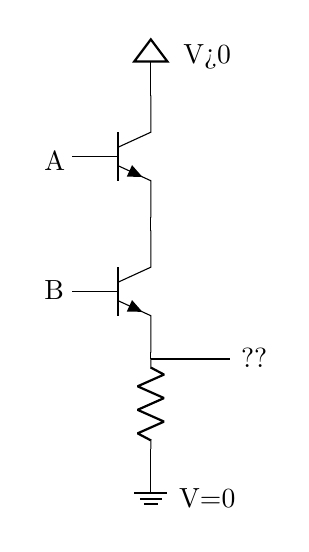
\begin{tikzpicture}
				% Paths, nodes and wires:
				\node[ground] at (1, 4.286){};
				\node[sground, yscale=-1] at (1, 9){};
				\node[shape=rectangle, minimum width=1.197cm, minimum height=0.679cm] at (1.812, 9.429){} node[anchor=north west, align=left, text width=0.809cm, inner sep=6pt] at (1.196, 9.786){V>0};
				\node[shape=rectangle, minimum width=0.608cm, minimum height=0.536cm] at (1.464, 3.857){} node[anchor=north west, align=left, text width=0.22cm, inner sep=6pt] at (1.143, 4.143){V=0};
				\node[npn] at (1, 8.143){};
				\node[npn] at (1, 6.429){};
				\draw (1, 5.571) to[american resistor, /tikz/circuitikz/bipoles/length=1.12cm] (1, 4.429);
				\draw (1, 9) -- (1, 8.913);
				\draw (1, 7.373) -- (1, 7.199);
				\draw (1, 5.659) -- (1, 5.571);
				\draw (1, 4.429) -- (1, 4.286);
				\draw (1, 5.571) -- (2, 5.571);
				\draw (0.16, 6.429) -- (0, 6.429);
				\draw (0.16, 8.143) -- (0, 8.143);
				\node[shape=rectangle, minimum width=0.679cm, minimum height=0.679cm] at (-0.214, 8.071){} node[anchor=north west, align=left, text width=0.291cm, inner sep=6pt] at (-0.571, 8.429){A};
				\node[shape=rectangle, minimum width=0.679cm, minimum height=0.679cm] at (-0.214, 6.429){} node[anchor=north west, align=left, text width=0.291cm, inner sep=6pt] at (-0.571, 6.786){B};
				\node[shape=rectangle, minimum width=0.679cm, minimum height=0.679cm] at (2.286, 5.571){} node[anchor=north west, align=left, text width=0.291cm, inner sep=6pt] at (1.929, 5.929){??};
			\end{tikzpicture}
		\end{column}
	\end{columns}
\end{frame}




\Subsection{Resistors}



\begin{frame}{What is a resistor?}
	light bulb

	ceramic

	the coils in your toaster

	something to soak up energy

	if you run electric current through it and it gets hot, it's a resistor (or at least has resistance)
\end{frame}


\begin{frame}{Voltage Drops in the Resistor}
	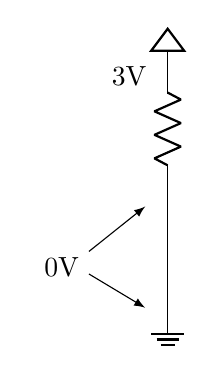
\begin{tikzpicture}
		% Paths, nodes and wires:
		\node[ground] at (2.571, 5.659){};
		\draw (2.571, 8.484) to[american resistor, /tikz/circuitikz/bipoles/length=1.12cm] (2.571, 7.199);
		\node[sground, yscale=-1] at (2.571, 8.484){};
		\node[shape=rectangle, minimum width=0.608cm, minimum height=0.536cm] at (1.964, 8.571){} node[anchor=north west, align=left, text width=0.22cm, inner sep=6pt] at (1.643, 8.857){3V};
		\node[shape=rectangle, minimum width=0.608cm, minimum height=0.536cm] at (1.107, 6.143){} node[anchor=north west, align=left, text width=0.22cm, inner sep=6pt] at (0.786, 6.429){0V};
		\draw[-latex] (1.571, 6.286) -- (2.286, 6.857);
		\draw[-latex] (1.571, 6) -- (2.286, 5.571);
		\draw (2.571, 7.199) -- (2.571, 5.659);
	\end{tikzpicture}
\end{frame}




\begin{frame}{Voltage only drops if it has somewhere to go}

Voltage drop only happens if electricity is flowing. Otherwise the voltage is the same everywhere

	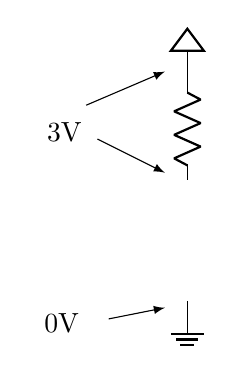
\begin{tikzpicture}
		% Paths, nodes and wires:
		\node[ground] at (2.571, 5.659){};
		\draw (2.571, 8.484) to[american resistor, /tikz/circuitikz/bipoles/length=1.12cm] (2.571, 7.199);
		\node[sground, yscale=-1] at (2.571, 8.484){};
		\node[shape=rectangle, minimum width=0.608cm, minimum height=0.536cm] at (0.893, 7.857){} node[anchor=north west, align=left, text width=0.22cm, inner sep=6pt] at (0.571, 8.143){3V};
		\node[shape=rectangle, minimum width=0.608cm, minimum height=0.536cm] at (0.857, 5.429){} node[anchor=north west, align=left, text width=0.22cm, inner sep=6pt] at (0.536, 5.714){0V};
		\draw[-latex] (1.286, 8.143) -- (2.286, 8.571);
		\draw[-latex] (1.429, 7.714) -- (2.286, 7.286);
		\draw[-latex] (1.571, 5.429) -- (2.286, 5.571);
	\end{tikzpicture}
\end{frame}


\begin{frame}{NOT ALLOWED}
	\begin{columns}
		\begin{column}{0.5\textwidth}
			We assume:
			\begin{itemize}
				\item Top rail fixed at V>0
				\item Bottom rail fixed at 0V
				\item Wires have zero resistance
			\end{itemize}
		\end{column}
		\begin{column}{0.5\textwidth}
			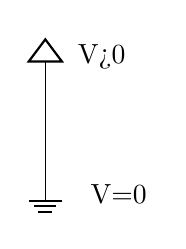
\begin{tikzpicture}
				% Paths, nodes and wires:
				\node[ground] at (1, 8){};
				\node[sground, yscale=-1] at (1, 9){};
				\node[shape=rectangle, minimum width=1.197cm, minimum height=0.679cm] at (1.813, 9.429){} node[anchor=north west, align=left, text width=0.809cm, inner sep=6pt] at (1.196, 9.786){V>0};
				\node[shape=rectangle, minimum width=0.608cm, minimum height=0.536cm] at (1.679, 7.714){} node[anchor=north west, align=left, text width=0.22cm, inner sep=6pt] at (1.357, 8){V=0};
				\draw (1, 9) -- (1, 8);
			\end{tikzpicture}		\end{column}
	\end{columns}

	If you try to build this, one of those assumptions will fail. What might that look like?

\end{frame}


\Subsection{Transistors}

\begin{frame}{Historical Transistors}
	\includegraphics[width=0.5\columnwidth]{images/tube-transistor-wiki}
\end{frame}


\begin{frame}{Modern Transistors}
	\includegraphics[width=\columnwidth]{images/semiconductor-transistor-overkill}
\end{frame}



\begin{frame}{Transistor Behavior}

	https://www.101computing.net/creating-logic-gates-using-transistors/

	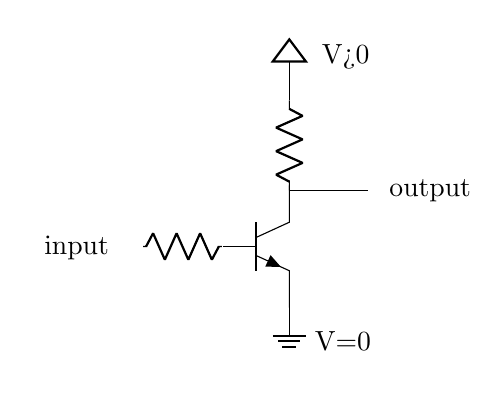
\begin{tikzpicture}
		% Paths, nodes and wires:
		\node[ground] at (1, 6.286){};
		\node[sground, yscale=-1] at (1, 9){};
		\node[shape=rectangle, minimum width=1.197cm, minimum height=0.679cm] at (1.813, 9.429){} node[anchor=north west, align=left, text width=0.809cm, inner sep=6pt] at (1.196, 9.786){V>0};
		\node[shape=rectangle, minimum width=0.608cm, minimum height=0.536cm] at (1.429, 5.857){} node[anchor=north west, align=left, text width=0.22cm, inner sep=6pt] at (1.107, 6.143){V=0};
		\draw (1, 8.857) to[american resistor, /tikz/circuitikz/bipoles/length=1.12cm] (1, 7.714);
		\draw (1, 9) -- (1, 8.857);
		\draw (1, 7.714) -- (2, 7.714);
		\node[shape=rectangle, minimum width=1.197cm, minimum height=0.679cm] at (2.67, 7.714){} node[anchor=north west, align=left, text width=0.809cm, inner sep=6pt] at (2.054, 8.071){output};
		\draw (-0.857, 7) to[american resistor, /tikz/circuitikz/bipoles/length=1.12cm] (0.143, 7);
		\draw (0.286, 7) -- (0.408, 7);
		\node[npn] at (1, 7){};
		\node[shape=rectangle, minimum width=1.197cm, minimum height=0.679cm] at (-1.714, 7){} node[anchor=north west, align=left, text width=0.809cm, inner sep=6pt] at (-2.33, 7.357){input};
	\end{tikzpicture}
\end{frame}


\begin{frame}{Transistor Behavior}
	\begin{columns}
		\begin{column}{0.5\textwidth}
			\usetikzlibrary{shapes.geometric}
			\begin{tikzpicture}
				% Paths, nodes and wires:
				\node[ground] at (1, 6.286){};
				\node[sground, yscale=-1] at (1, 9){};
				\node[shape=rectangle, minimum width=1.197cm, minimum height=0.679cm] at (1.813, 9.429){} node[anchor=north west, align=left, text width=0.809cm, inner sep=6pt] at (1.196, 9.786){V>0};
				\node[shape=rectangle, minimum width=0.608cm, minimum height=0.536cm] at (1.429, 5.857){} node[anchor=north west, align=left, text width=0.22cm, inner sep=6pt] at (1.107, 6.143){V=0};
				\draw (1, 8.857) to[american resistor, /tikz/circuitikz/bipoles/length=1.12cm] (1, 7.714);
				\node[shape=ellipse, draw, line width=1pt, dash pattern={on 1pt off 2pt}, minimum width=1.149cm, minimum height=1.108cm] at (1, 7){};
				\node[shape=rectangle, minimum width=1.197cm, minimum height=0.965cm] at (-1.33, 7.143){} node[anchor=north west, align=left, text width=0.809cm, inner sep=6pt] at (-1.946, 7.643){input\\V>0};
				\draw (1, 6.571) to[cute closed switch] (1, 7.429);
				\draw (1, 9) -- (1, 8.857);
				\draw (1, 7.714) -- (1, 7.429);
				\draw (1, 6.571) -- (1, 6.286);
				\draw (1, 7.714) -- (2, 7.714);
				\node[shape=rectangle, minimum width=1.197cm, minimum height=0.679cm] at (2.67, 7.714){} node[anchor=north west, align=left, text width=0.809cm, inner sep=6pt] at (2.054, 8.071){??};
				\draw (-0.714, 7) to[american resistor, /tikz/circuitikz/bipoles/length=1.12cm] (0.286, 7);
				\draw (0.286, 7) -- (0.408, 7);
			\end{tikzpicture}
		\end{column}
		\begin{column}{0.5\textwidth}
			\usetikzlibrary{shapes.geometric}
			\begin{tikzpicture}
				% Paths, nodes and wires:
				\node[ground] at (1, 6.286){};
				\node[sground, yscale=-1] at (1, 9){};
				\node[shape=rectangle, minimum width=1.197cm, minimum height=0.679cm] at (1.813, 9.429){} node[anchor=north west, align=left, text width=0.809cm, inner sep=6pt] at (1.196, 9.786){V>0};
				\node[shape=rectangle, minimum width=0.608cm, minimum height=0.536cm] at (1.429, 5.857){} node[anchor=north west, align=left, text width=0.22cm, inner sep=6pt] at (1.107, 6.143){V=0};
				\draw (1, 8.857) to[american resistor, /tikz/circuitikz/bipoles/length=1.12cm] (1, 7.714);
				\node[shape=ellipse, draw, line width=1pt, dash pattern={on 1pt off 2pt}, minimum width=1.149cm, minimum height=1.108cm] at (1, 7){};
				\node[shape=rectangle, minimum width=1.197cm, minimum height=0.965cm] at (-1.33, 7.143){} node[anchor=north west, align=left, text width=0.809cm, inner sep=6pt] at (-1.946, 7.643){input\\V=0};
				\draw (1, 6.571) to[cute open switch] (1, 7.429);
				\draw (1, 9) -- (1, 8.857);
				\draw (1, 7.714) -- (1, 7.429);
				\draw (1, 6.571) -- (1, 6.286);
				\draw (1, 7.714) -- (2, 7.714);
				\node[shape=rectangle, minimum width=1.197cm, minimum height=0.679cm] at (2.67, 7.714){} node[anchor=north west, align=left, text width=0.809cm, inner sep=6pt] at (2.054, 8.071){??};
				\draw (-0.714, 7) to[american resistor, /tikz/circuitikz/bipoles/length=1.12cm] (0.286, 7);
				\draw (0.286, 7) -- (0.408, 7);
			\end{tikzpicture}
		\end{column}
	\end{columns}
\end{frame}


\begin{frame}{Transistor Behavior}
	\begin{columns}
		\begin{column}{0.5\textwidth}
			\usetikzlibrary{shapes.geometric}
			\begin{tikzpicture}
				% Paths, nodes and wires:
				\node[ground] at (1, 6.286){};
				\node[sground, yscale=-1] at (1, 9){};
				\node[shape=rectangle, minimum width=1.197cm, minimum height=0.679cm] at (1.813, 9.429){} node[anchor=north west, align=left, text width=0.809cm, inner sep=6pt] at (1.196, 9.786){V>0};
				\node[shape=rectangle, minimum width=0.608cm, minimum height=0.536cm] at (1.429, 5.857){} node[anchor=north west, align=left, text width=0.22cm, inner sep=6pt] at (1.107, 6.143){V=0};
				\draw (1, 8.857) to[american resistor, /tikz/circuitikz/bipoles/length=1.12cm] (1, 7.714);
				\node[shape=ellipse, draw, line width=1pt, dash pattern={on 1pt off 2pt}, minimum width=1.149cm, minimum height=1.108cm] at (1, 7){};
				\node[shape=rectangle, minimum width=1.197cm, minimum height=0.965cm] at (-1.33, 7.143){} node[anchor=north west, align=left, text width=0.809cm, inner sep=6pt] at (-1.946, 7.643){input\\V>0};
				\draw (1, 6.571) to[cute closed switch] (1, 7.429);
				\draw (1, 9) -- (1, 8.857);
				\draw (1, 7.714) -- (1, 7.429);
				\draw (1, 6.571) -- (1, 6.286);
				\draw (1, 7.714) -- (2, 7.714);
				\node[shape=rectangle, minimum width=1.197cm, minimum height=0.679cm] at (2.67, 7.714){} node[anchor=north west, align=left, text width=0.809cm, inner sep=6pt] at (2.054, 8.071){output\\V=0};
				\draw (-0.714, 7) to[american resistor, /tikz/circuitikz/bipoles/length=1.12cm] (0.286, 7);
				\draw (0.286, 7) -- (0.408, 7);
			\end{tikzpicture}
		\end{column}
		\begin{column}{0.5\textwidth}
			\usetikzlibrary{shapes.geometric}
			\begin{tikzpicture}
				% Paths, nodes and wires:
				\node[ground] at (1, 6.286){};
				\node[sground, yscale=-1] at (1, 9){};
				\node[shape=rectangle, minimum width=1.197cm, minimum height=0.679cm] at (1.813, 9.429){} node[anchor=north west, align=left, text width=0.809cm, inner sep=6pt] at (1.196, 9.786){V>0};
				\node[shape=rectangle, minimum width=0.608cm, minimum height=0.536cm] at (1.429, 5.857){} node[anchor=north west, align=left, text width=0.22cm, inner sep=6pt] at (1.107, 6.143){V=0};
				\draw (1, 8.857) to[american resistor, /tikz/circuitikz/bipoles/length=1.12cm] (1, 7.714);
				\node[shape=ellipse, draw, line width=1pt, dash pattern={on 1pt off 2pt}, minimum width=1.149cm, minimum height=1.108cm] at (1, 7){};
				\node[shape=rectangle, minimum width=1.197cm, minimum height=0.965cm] at (-1.33, 7.143){} node[anchor=north west, align=left, text width=0.809cm, inner sep=6pt] at (-1.946, 7.643){input\\V=0};
				\draw (1, 6.571) to[cute open switch] (1, 7.429);
				\draw (1, 9) -- (1, 8.857);
				\draw (1, 7.714) -- (1, 7.429);
				\draw (1, 6.571) -- (1, 6.286);
				\draw (1, 7.714) -- (2, 7.714);
				\node[shape=rectangle, minimum width=1.197cm, minimum height=0.679cm] at (2.67, 7.714){} node[anchor=north west, align=left, text width=0.809cm, inner sep=6pt] at (2.054, 8.071){output\\V>0};
				\draw (-0.714, 7) to[american resistor, /tikz/circuitikz/bipoles/length=1.12cm] (0.286, 7);
				\draw (0.286, 7) -- (0.408, 7);
			\end{tikzpicture}
		\end{column}
	\end{columns}
\end{frame}



\begin{frame}{Why two resistors?}

In many cases, we can get away with just one resistor. The previous example had two. Why?

Always need a resistor between a voltage source and ground. Transistors have internal resistance but it's very small. Easy to burn them out

\end{frame}





\begin{frame}{More Complex Example}
	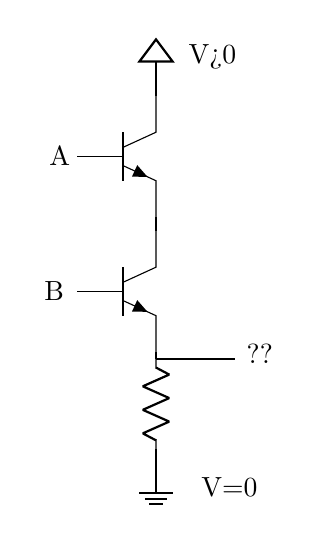
\begin{tikzpicture}
		% Paths, nodes and wires:
		\node[ground] at (1, 4.286){};
		\node[sground, yscale=-1] at (1, 9){};
		\node[shape=rectangle, minimum width=1.197cm, minimum height=0.679cm] at (1.813, 9.429){} node[anchor=north west, align=left, text width=0.809cm, inner sep=6pt] at (1.196, 9.786){V>0};
		\node[shape=rectangle, minimum width=0.608cm, minimum height=0.536cm] at (1.679, 4){} node[anchor=north west, align=left, text width=0.22cm, inner sep=6pt] at (1.357, 4.286){V=0};
		\draw (1, 5.571) to[american resistor, /tikz/circuitikz/bipoles/length=1.12cm] (1, 4.429);
		\node[npn] at (1, 8.143){};
		\node[npn] at (1, 6.429){};
		\draw (1, 9) -- (1, 8.913);
		\draw (1, 7.373) -- (1, 7.199);
		\draw (1, 5.659) -- (1, 5.571);
		\draw (1, 5.571) -- (2, 5.571);
		\draw (0.16, 8.143) -- (0, 8.143);
		\draw (0.16, 6.429) -- (0, 6.429);
		\draw (1, 4.429) -- (1, 4.286);
		\node[shape=rectangle, minimum width=0.668cm, minimum height=0.65cm] at (-0.22, 8.143){} node[anchor=north west, align=left, text width=0.28cm, inner sep=6pt] at (-0.571, 8.485){A};
		\node[shape=rectangle, minimum width=0.668cm, minimum height=0.65cm] at (-0.286, 6.429){} node[anchor=north west, align=left, text width=0.28cm, inner sep=6pt] at (-0.637, 6.771){B};
		\node[shape=rectangle, minimum width=0.668cm, minimum height=0.65cm] at (2.286, 5.628){} node[anchor=north west, align=left, text width=0.28cm, inner sep=6pt] at (1.934, 5.971){??};
	\end{tikzpicture}
\end{frame}




% what is a transistor
% building logic gates

% TEST 3 TOPICS

\Section{Instruction Pipelining}

\Subsection{FDEW Cycle}

\Subsection{Pipelining}

\Subsection{Hazards}

% pipelining
% data hazards
% control hazards

\Section{Assembly Conditionals and Loops}

% b, beq, bne, ...
% if/else
% while loops
% for loops

\input{sections/multiprocessing.tex}
% booting
% forking
% threads, cores, processes
% async


\Section{Appendix}


\Subsection{Raspberry Pi Setup}


\begin{frame}{Pi Setup: Kit Contents}
	\begin{columns}
		\begin{column}{0.5\textwidth}
			\begin{enumerate}
				\item Pi case
				\item Raspberry Pi (in box)
				\item Heat sinks
				\item Power cord
				\item Ethernet to USB adapter
				\item Ethernet cord
				\item USB 2 to USB 3 adapter
				\item SD Card
				\item Accessory case
			\end{enumerate}
		\end{column}
		\begin{column}{0.5\textwidth}
			\includegraphics[width=\columnwidth]{images/pi-kit-contents}
		\end{column}
	\end{columns}
\end{frame}


\begin{frame}{Pi Setup: Apply Heat Sinks}
	\begin{columns}
		\begin{column}{0.5\textwidth}
			\includegraphics[width=\columnwidth]{images/pi-heat-sinks-1}
		\end{column}
		\begin{column}{0.5\textwidth}
			\includegraphics[width=\columnwidth]{images/pi-heat-sinks-2}
		\end{column}
	\end{columns}
\end{frame}

\begin{frame}{Pi Setup: Apply Nonslip Nubs}
	\includegraphics[width=\columnwidth]{images/pi-case-nubs}
\end{frame}

\begin{frame}{Pi Setup: Install in Case}
	\includegraphics[width=\columnwidth]{images/pi-in-case}
\end{frame}

\begin{frame}{Pi Setup: SD Card}
	\begin{columns}
		\begin{column}{0.5\textwidth}
			\includegraphics[width=\columnwidth]{images/pi-sd-card-1}
		\end{column}
		\begin{column}{0.5\textwidth}
			\includegraphics[width=\columnwidth]{images/pi-sd-card-2}
		\end{column}
	\end{columns}
\end{frame}

\begin{frame}{Pi Setup: Connect to Laptop}
	\includegraphics[width=\columnwidth]{images/pi-to-laptop}
\end{frame}

\begin{frame}{Pi Setup: Connect to Power}
\end{frame}

\begin{frame}{Laptop Setup: Enable WiFi}
	\includegraphics[width=\columnwidth]{images/pi-network-settings}
\end{frame}

\begin{frame}{Laptop Setup: Install VSCode}
	\includegraphics[width=\columnwidth]{images/vscode-remote-ssh}
\end{frame}

\begin{frame}{Laptop Setup: Add Remote Connection}
	\includegraphics[width=\columnwidth]{images/vscode-add-remote}
\end{frame}

\begin{frame}{Laptop Setup: SSH Login}
	\begin{itemize}
		\item Default username/password is raspberri/pi
		\item Make sure to update username and password
	\end{itemize}
\end{frame}


\Subsection{CSGit Setup}

% vscode setup
% pi setup
% csgit setup


\end{document}
% boolean operators
% boolean expressions
% boolean circuits
% resistors & transistors


\documentclass{beamer}
\usepackage[utf8]{inputenc}
\usepackage[T1]{fontenc}
\usepackage{circuitikz}

\usepackage{multirow}

\title{CS241: Hardware Design}
\date{\today}
\author[Fyfe and Lynn]{Charles Fyfe and Melissa Lynn}
\institute{St Olaf College}

\usetheme{grape}

\usepackage{parskip}
\usepackage{multicol}
\usepackage{graphicx}
% make \oplus look nice
\usepackage{amssymb}

\begin{document}


\titlepage

% just sections up top
\setcounter{tocdepth}{1}

\begin{frame}{Outline}

	\begin{multicols*}{2}
		\tableofcontents
	\end{multicols*}
\end{frame}

% show subsections later
\setcounter{tocdepth}{2}


\Section{Syllabus}

\begin{frame}{Course Overview}

	\includegraphics[width=\columnwidth]{images/dune-robot-hbo}

	{\center
		Thou shalt not make a machine in the likeless of a human mind
	}

	{\small \hfill
		The Orange Catholic Bible, Dune, Frank Herbert
	}
\end{frame}


\begin{frame}{Course Overview}

	Computers feel like magic. You type words. The machine does complex things. Especially in the era of large language models

	But it's not magic. Computers are made of semiconductors, metal, and magnets. Three different kinds of rocks

	This course is about demystifying the machine and exploring how, fundamentally, computers do what they do. Specifically, we'll be looking at:
	\begin{itemize}
		\item The fundamental components of a computer
		\item How data is stored on a computer
		\item Building electrical circuits to perform logic
		\item Programming in Assembly (a very low-level language)
	\end{itemize}
\end{frame}

\Subsection{Grading}

\begin{frame}{Course Grade Breakdown}
	\begin{itemize}
		\item Quizzes and final: 45\%
		\item Homework and labs: 45\%
		\item Participation: 10\%
	\end{itemize}
\end{frame}

\begin{frame}{Standards-Based Grading}
	\begin{itemize}
		\item There are nine standards in the class. Each is worth 5\% of your grade.
		\item There are three quizzes. Each quiz covers three standards.
		\item The final covers all nine standards.
		\item If you demonstrate proficiency on the quiz, you're done with that standard. Full credit. You can skip that part of the final.
		\item If you demonstrate partial proficiency on the quiz, you get half credit. Try again on the final for full credit.
		\item If you do not demonstrate proficiency on the quiz, you get no credit. You can still get full credit on the final!
	\end{itemize}
\end{frame}


\begin{frame}{Homework and Labs}
	\begin{itemize}
		\item One or more lab exercises for each standard. We start these together in class. You may need to finish on your own time.
		\item We will have a homework assignment for each standard.
		\item Please work together in small groups.
		\item Please ensure that the work you turn in reflects your own understanding.
	\end{itemize}
\end{frame}

\begin{frame}{Late Work Policy}
	Please try to get your work in on time.
	\begin{itemize}
		\item If you don't get your work done on time, you may fall behind in the class.
		\item Late work is inconvenient for the TAs. They will be grumpy and vindictive when they grade your work.
		\item TAs will have their own finals to worry about! Late work at the end of the semester might be refused.
	\end{itemize}
	If you need an extension, please reach out beforehand.
\end{frame}

\begin{frame}{Peer Reviews}
	\begin{itemize}
		\item Participation score (10\% of your total grade) is mostly based on peer reviews.
		\item Reviews will be short. Less than one page.
		\item You can get full credit here without too much trouble. Show up. Work together. Make it easy for your peers to say nice things about you.
		\item I recommend keeping notes over the course of the semester when someone is particularly helpful, insightful, etc. Good reviews have concrete examples.
	\end{itemize}
\end{frame}

\Subsection{Office Hours}

\begin{frame}{Office Hours}
	TODO
\end{frame}


\Subsection{Disability Accommodations}

\begin{frame}{Disability Accommodations}
	I am committed to supporting the learning of all students in my class. If you have already
	registered with Disability and Access (DAC) and have your letter of accommodations, please
	meet with me as soon as possible to discuss, plan, and implement your accommodations in the
	course. If you have or think you have a disability (learning, sensory, physical, chronic health,
	mental health or attentional), please contact Disability and Access staff at 507-786-3288 or by visiting \href{https://wp.stolaf.edu/academic-support/dac}{their website}.


	If you have an accommodation that allows you extra time or a low distraction environment for
	quizzes and exams, please email me at least three days before each quiz or exam, so that I can
	make sure to reserve a room.
\end{frame}


\Subsection{Religious Accommodations}

\begin{frame}{Religious Accommodations}
	As part of my commitment to make St Olaf an inclusive community, I will provide students with
	reasonable religious accommodations. If you will be missing class for a religious observance or
	require another religious accommodation, please meet with me to discuss these.
\end{frame}


\Subsection{Academic Integrity}

\begin{frame}{Academic Integrity}

	Plagiarism is a serious academic offense. Hand in your own work. Give credit appropriately when you draw from the work of others. For more information please see:

	\begin{itemize}
		\item \href{https://wp.stolaf.edu/facultyhandbook/academic-integrity-faculty-handbook-category-2}{Faculty Handbook: Academic Integrity}
		\item \href{https://wp.stolaf.edu/honorcouncil/}{The Honor Code}
		\item \href{https://wp.stolaf.edu/roadmap-to-academic-integrity}{Roadmap to Academic Integrity}
	\end{itemize}

	Work that violates this policy will typically receive no credit. In especially serious cases the penalty can be an F in the course.
\end{frame}

\Subsection{AI Use Policy}

\begin{frame}{AI Usage Policy}
	Please not submit AI work as your own.

	You may use AI tools when studying, but be careful. These tools are very good with mainstream languages like Python. We're working with Assembly, which is very much \textbf{not} a mainstream language.

\end{frame}


\Subsection{St Olaf Land Acknowledgement}

\begin{frame}{St Olaf Land Acknowledgement}
	We stand on the homelands of the Wahpekute Band of the Dakota Nation. We honor with
	gratitude the people who have stewarded the land throughout the generations and their ongoing
	contributions to this region. We acknowledge the ongoing injustices that we have committed
	against the Dakota Nation, and we wish to interrupt this legacy, beginning with acts of healing
	and honest storytelling about this place.

	For more information about land acknowledgement statements at St Olaf, please see \href{https://wp.stolaf.edu/education/land-acknowledgement/}{here} and \href{https://wp.stolaf.edu/equity-inclusion/land-acknowledgement/}{here}.
\end{frame}


\Subsection{Statement of Inclusivity}

\begin{frame}{Statement of Inclusivity}
	In keeping with St. Olaf College's mission statement, this class strives to be an inclusive
	learning community, respecting those of differing backgrounds and beliefs. As a community, we
	aim to be respectful to all citizens in this class, regardless of race, ethnicity, religion, gender or
	sexual orientation.
\end{frame}


\Subsection{Gender Pronouns}

\begin{frame}{Gender Pronouns}
	This course affirms people of all gender expressions and gender identities. If you go by a
	different name than what is on the class roster, please let me know.

	Using correct gender
	pronouns is important to me, so you are encouraged to share your pronouns with me and
	correct me if a mistake is made. If you have any questions or concerns, please do not hesitate
	to contact me.
\end{frame}


\Subsection{Multilingual Student Support}

\begin{frame}{Multilingual Student Support}
	I am committed to making course content accessible to all students. If English is not your first
	language and this causes you concern about the course, please speak with me. Students who
	would like extra support with writing or speaking in English can also contact the language support specialist (\href{mailto:berryag@stolaf.edu}{berryag@stolaf.edu}) in the Academic Success Center.
\end{frame}


\Subsection{Mental Health}

\begin{frame}{Mental Health}

	I greatly value your experience in this class, and it is my duty to facilitate a safe, caring, and
	productive learning environment.

	I recognize that you may experience a range of emotional, physical, and/or psychological
	issues, both in and out of the classroom, that may distract you from your learning.

	If you are experiencing such issues, please do not hesitate to come see me. I am here to listen.
	We can also discuss what further resources might be available to you.
\end{frame}

\Subsection{Required Referrals}


\begin{frame}{Required Referrals}
	You are welcome to talk to me about circumstances outside the course that
	affect your classroom experience or acadmic performance. However, please keep
	in mind that I am required to refer cases of discrimination, harassment,
	sexual misconduct, and violence.

	Here are some resources where you can share privately:

	\begin{itemize}
		\item Boe House Counseling Center
		\item College Pastors and Chaplains
		\item Sexual Assault Resource Network (SARN)
		\item Health Services
		\item TimelyCare
	\end{itemize}
\end{frame}




\Subsection{St. Olaf Pride Statement}

\begin{frame}{St. Olaf Pride Statement}
	As an Ole, I will practice:
	\begin{itemize}
		\item Passion for learning and pursuit of vocation
		\item Respect for the worth and dignity of all people
		\item Integrity at all times, in all circumstances
		\item Dedication to a life of service, and
		\item Engagement with my community and the world.
	\end{itemize}
\end{frame}









\Subsection{Important Links}

\begin{frame}{Important Links}
	\begin{itemize}
		\item ARM tutorial https://computerscience.chemeketa.edu/armTutorial/index.html
		\item ARM simulator https://cpulator.01xz.net/?sys=arm
		\item circuit simulator: https://circuitverse.org/simulator
	\end{itemize}
\end{frame}





% TEST 1 TOPICS


\Section{Data Representation}

\begin{frame}{How do computers store information?}
	Computers work using electrical signals which can be on or off. If we let:
	\begin{itemize}
		\item On means 1
		\item Off means 0
	\end{itemize}
	We can use sequences of 0s and 1s to represent information
\end{frame}

\Subsection{Positive Integers in Binary}

\begin{frame}{Numbers in Base Ten (aka Decimal)}
	Let's start by talking about how we write numbers normally.

	For example, let's look at the number 109:
	\begin{align*}
		109 & = 100 \;+\; 0 \;+\; 9                                   \\
		    & = 1 \Times 10^2 \;+\; 0 \Times 10^1 \;+\; 9 \Times 10^0
	\end{align*}
	This way of writing numbers is called base ten.
	We use ten digits (0 to 9 inclusive) and each position in the number is scaled by a power of ten.

	In terms of math, there is nothing special about base ten. We probably use it
	because we have ten fingers. Some ancient civilizations used sompletely
	different systems for counting!
\end{frame}

\begin{frame}{Numbers in Base Two (aka Binary)}
	Computers don't have fingers. They express everything as sequences of 1s and 0s. This format is called binary:

	\begin{align*}
		0b1101101 & =
		1 \Times 2^6 +
		1 \Times 2^5 +
		0 \Times 2^4 +
		1 \Times 2^3 +
		1 \Times 2^2 +
		0 \Times 2^1 +
		1 \Times 2^0                              \\
		          & = 64 + 32 + 0 + 8 + 4 + 0 + 1 \\
		          & = 109                         \\
	\end{align*}
	Importantly: we always use the prefix ``0b'' to avoid confusion when writing numbers in binary.

	1101 is one thousand one hundred and one

	0b1101 is thirteen
\end{frame}

\begin{frame}{Converting from Decimal to Binary}

	If the number is odd, append a 1 on the left. Otherwise, append a 0. Then
	divide your decimal number by two and ignore any remainder. Repeat until your
	decimal number is zero. \\

	For example, starting with 58:

	\begin{itemize}
		\item 58 is even, so append \Highlight{0}. Divide by two, leaving 29.
		\item 29 is odd, so append \Highlight{1}0. Divide by two, leaving 14.
		\item 14 is even, so append \Highlight{0}10. Divide by two, leaving 7.
		\item 7 is odd, so append \Highlight{1}010. Divide by two, leaving 3.
		\item 3 is odd, so append \Highlight{1}1010. Divide by two, leaving 1.
		\item 1 is odd, so append \Highlight{1}11010. Divide by two, leaving 0.
	\end{itemize}

	So 58 in binary is 0b111010.

\end{frame}

\begin{frame}{Converting from Binary to Decimal}

	We can confirm by converting back. The rightmost bit is worth 1, then 2, then
	4, and so on:

	\begin{align*}
		0b111010 & =
		1 \Times 2^5 +
		1 \Times 2^4 +
		1 \Times 2^3 +
		0 \Times 2^2 +
		1 \Times 2^1 +
		0 \Times 2^0                          \\
		         & = 32 + 16  + 8 + 0 + 2 + 0 \\
		         & = 58
	\end{align*}

\end{frame}

\begin{frame}{Addition in Binary}
	Binary addition works just like decimal addition.
	Start from the right, add straight down, and carry when you run out of digits.

	For example:
	\[
		\begin{array}{ccccccccc}
			1 & 1 & 1 & 1 & 1 &   &   &   &   \\
			  & 0 & 0 & 1 & 1 & 1 & 0 & 0 & 0 \\
			+ & 1 & 1 & 1 & 0 & 1 & 0 & 0 & 1 \\
			\hline
			1 & 0 & 0 & 1 & 0 & 0 & 0 & 0 & 1 \\
		\end{array}
	\]

	What happens if we try to perform this operation but we only have 8 bits to
	store the answer?
\end{frame}

\begin{frame}{Multiplication in Binary}
	Binary multiplication works just like decimal multiplication.
	Multiply the top number by the rightmost digit of the bottom number.
	Then move to the next line, add a zero, and repeat for the next digit.
	Finally, add up the lines. For example:
	\[
		\begin{array}{cccccc}
			  &   &        & 1 & 1 & 0 \\
			  &   & \times & 1 & 0 & 1 \\
			\hline
			  &   &        & 1 & 1 & 0 \\
			  &   & 0      & 0 & 0 & 0 \\
			+ & 1 & 1      & 0 & 0 & 0 \\
			\hline
			  & 1 & 1      & 1 & 1 & 0 \\
		\end{array}
	\]
\end{frame}

\begin{frame}{Division in Binary}
	To divide by 2, shift the bits one place to the right. \\

	To divide by 4, shift the bits two places to the right. \\

	That's about as deep as we go in this class. If you're curious to learn more,
	see the textbook.

\end{frame}



\Subsection{Hexadecimal}

\begin{frame}{What? Why?}

	Binary is how machines store data. But writing out binary by hand is a chore.
	In practice, it's often convenient to use hexadecimal (base 16) instead.

	\begin{itemize}
		\item Decimal uses ten digits, 0-9
		\item Binary uses two digits, 0 and 1
		\item Hexadecimal uses sixteen digits: 0-9 along with A-F
	\end{itemize}
	Hexadecimal values are always prefixed with ``0x'' to avoid ambiguity.
\end{frame}

\begin{frame}{Converting Between Binary and Hexadecimal}

	Converting back and forth between binary and hexadecimal does not require any
	math! Every four bits become one hex digit.
	\begin{align*}
		0b0000 & = 0x0 = 0 & 0b1000 & = 0x8 = 8  \\
		0b0001 & = 0x1 = 1 & 0b1001 & = 0x9 = 9  \\
		0b0010 & = 0x2 = 2 & 0b1010 & = 0xA = 10 \\
		0b0011 & = 0x3 = 3 & 0b1011 & = 0xB = 11 \\
		0b0100 & = 0x4 = 4 & 0b1100 & = 0xC = 12 \\
		0b0101 & = 0x5 = 5 & 0b1101 & = 0xD = 13 \\
		0b0110 & = 0x6 = 6 & 0b1110 & = 0xE = 14 \\
		0b0111 & = 0x7 = 7 & 0b1111 & = 0xF = 15 \\
	\end{align*}
\end{frame}

\begin{frame}{Converting Hexadecimal to Decimal}

	Hexadecimal is base 16. So each place corresponds to a power of 16.

	\begin{align*}
		0x3AB & = 3 \times 16^2 + 10 \times 16^1 + 11 \times 16^0 \\
		      & = 3 \times 256 + 10 \times 16 + 11 \times 1       \\
		      & = 768 + 160 + 11                                  \\
		      & = 954                                             \\
	\end{align*}

	Hexadecimal is very compact! These numbers get big fast

\end{frame}

\begin{frame}{Arithmetic in Hexadecimal}

	Addition and multiplication work in hexadecimal just like they do in binary and
	decimal. Just be careful about carrying.

	\[
		\begin{array}{ccccc}
			1 &   &   & 1 &   \\
			  & 4 & 1 & 7 & B \\
			+ & C & 2 & 0 & F \\
			\hline
			1 & 0 & 3 & 8 & A \\
		\end{array}
	\]

\end{frame}






\Subsection{Negatives in Binary}

\begin{frame}{First Attempt: Signed Magnitude}

	We can use the first digit to hold the sign, then the rest of the digits to
	hold magnitue:

	\begin{itemize}
		\item 0b\Highlight{0}1011001 is positive 10110001, so 89
		\item 0b\Highlight{1}1011001 is negative 1011001, so -89
	\end{itemize}

	This is nice and straightforward!

\end{frame}

\begin{frame}{Addition and Subtraction with Signed Magnitude}
	Adding positive numbers works just the same. But what happens if we throw a minus sign in there?

	For example, let's look at 12 - 5. First, rewrite it as 12 + (-5). Then:

	\[
		\begin{array}{ccccccccc}
			  & 0 & 0 & 0 & 0 & 1 & 1 & 0 & 0 \\
			+ & 1 & 0 & 0 & 0 & 0 & 1 & 0 & 1 \\
			\hline
			  & ? & ? & ? & ? & ? & ? & ? & ? \\
		\end{array}
	\]

	We know the result should be 7 (0b00000111). But our regular rules for addition
	do not get us there.
\end{frame}

\begin{frame}{Zero with Signed Magnitude}

	Using signed magnitude, 0b00000000 is zero.

	And 0b10000000 is negative zero (which is also zero).

	Using this convention, we have to worry about the difference between numerical
	equality and bitwise equality. That seems pretty messy.
\end{frame}

\begin{frame}{Can We Do Better?}
	Signed magnitude was a swing and a miss. What do we want when we talk about negative numbers?
	\begin{itemize}
		\item We want positive numbers to work like we expect
		\item We want 0b00000000 to be zero, with no ambiguity
		\item We want addition and subtraction to work the same for positive and negative
	\end{itemize}
\end{frame}

\begin{frame}{Another Idea: Two's Complement}
	We know 1 - 1 = 0. Put another way, 1 + (-1) = 0. Can we work backwards from there to figure out how to write -1?
	\[
		\begin{array}{ccccccccc}
			  & 0 & 0 & 0 & 0 & 0 & 0 & 0 & 1 \\
			+ & 1 & 1 & 1 & 1 & 1 & 1 & 1 & 1 \\
			\hline
			  & 0 & 0 & 0 & 0 & 0 & 0 & 0 & 0 \\
		\end{array}
	\]

	Remember: on a computer, our numbers have to fit in a set number of bits.
	Anything past that gets thrown away. This is called overflow. In this case,
	overflow works in our favor!
\end{frame}

\begin{frame}{Working Backwards from Zero}
	We can use the same trick to identify the rest of the negative numbers:
	\begin{itemize}
		\item 0b00000000 is 0
		\item 0b11111111 is -1
		\item 0b11111110 is -2
		\item 0b11111101 is -3
		\item 0b11111100 is -4
		\item etc
	\end{itemize}

\end{frame}

\begin{frame}{The Sign Bit (Again)}
	We only have 256 possible integers. How do we decide where the positives end and the negatives begin?

	Unsigned int: bits are worth 1, 2, 4, 8, 16, 32, 64, 128

	Signed magnitude: bits are worth $\pm1, \pm2, \pm4, \pm8, \pm16, \pm32, \pm64$,
	and the last bit tells us whether to use positive or negative (yikes)

	Two's complement: bits are worth 1, 2, 4, 8, 16, 32, 64, \Highlight{-128}

	Range of possible values is -128 to 127.
\end{frame}

\begin{frame}{Flipping Signs in Two's Complement}
	To flip the sign of a two's complement integer, flip all the bits then add 1. Ignore the overflow (if any). This works for both positive and negative numbers.

	For example:
	\begin{itemize}
		\item 55 is 0b01010111
		\item Flip the bits: 0b10101000, then add 1: 0b10101001
		\item So -55 is 0b10101001
		\item Flip the bits again: 0b01010110, add 1: 0b01010111
		\item So -(-55) = 55 = 0b01010111
	\end{itemize}

	What happens if we negate zero?
\end{frame}

\begin{frame}{Overflow}
	Overflow is important for two's complement. It ensures that positive zero and negative zero are the same. But it is also a constraint!

	Try adding 0b01101001 + 0b01011010:
	\[
		\begin{array}{ccccccccc}
			  &   & 1 & 1 & 1 &   &   &   &   \\
			  & 0 & 1 & 1 & 0 & 1 & 0 & 0 & 1 \\
			+ & 0 & 1 & 0 & 1 & 1 & 0 & 1 & 0 \\
			\hline
			  & 1 & 1 & 0 & 0 & 0 & 0 & 1 & 1 \\
		\end{array}
	\]

	These are two's complement numbers. Convert them to decimal. What just
	happened?

\end{frame}


\Subsection{Fractions and Decimals}

\begin{frame}{The Decimal Point}

	Sometimes we need to store numbers that aren't integers. \\

	Before we worry about binary, what does 21.867 mean? \\

	\begin{align*}
		21.867 & = 2 \Times 10^1 + 1 \Times 10^0 + 8 \Times ?? + 6 \Times ?? + 7 \Times ??
	\end{align*}

\end{frame}

\begin{frame}{The Decimal Point}

	In decimal:
	\begin{align*}
		21.867 & = 2 \Times 10^1 + 1 \Times 10^0 + 8 \Times 10^{-1} + 6 \Times 10^{-2} + 7 \Times 10^{-3}             \\
		       & =2 \Times 10 + 1 \Times 1 + 8 \Times \frac{1}{10} + 6 \Times \frac{1}{100} + 7 \Times \frac{1}{1000} \\
	\end{align*}

	In binary, we can use the same idea:
	\begin{align*}
		0b101.010 & = 1 \Times 2^2 + 0 \Times 2^1 + 1 \Times 2^0 + 0 \Times 2^{-1} + 1 \Times 2^{-2} + 0 \Times 2^{-3} \\
		          & = 1 \Times 4 + 0 + 1 \Times 1 + 0 + 1 \Times \frac{1}{4} + 0                                       \\
		          & = 5.25                                                                                             \\
	\end{align*}

\end{frame}

\begin{frame}{Fixed Point Representation}

	The computer just stores 1s and 0s, not decimal points. How do we distinguish
	these values?
	\begin{itemize}
		\item 0b0101110.1 = 46.5
		\item 0b010111.01 = 23.25
		\item 0b01011.101 = 11.625
	\end{itemize}

	One option is to specify the location of the decimal point ahead of time. For
	example, we could say that our eight-bit binary decimal always has two decimal
	bits. \\

	What is an upside of this approach? What is a downside?

\end{frame}

\begin{frame}{Floating Point Representation}

	Floating point numbers are a bit more complicated, but much more flexible. For
	a 16-bit floating point number we get:

	\begin{itemize}
		\item 1 bit for the sign
		\item 5 bits for the exponent (value -14 to 15)
		\item 10 bits for the significand (value 0 to 1023)
	\end{itemize}

	To turn those components into a value we use:
	\begin{align*}
		\text{value} & = (-1)^{\text{sign}} \times 2^{\text{exponent} - 15} \times \left(1 + \frac{\text{significand}}{1024} \right)
	\end{align*}

	Why offset the exponent?

	Why add 1 to the significand fraction?

\end{frame}

% Explanation here for the 127 offset: https://www.quora.com/Why-do-we-add-127-to-the-exponent-in-IEEE-754-floating-number-format-to-get-the-actual-exponent-value

\begin{frame}{Floating Point Examples}

	\begin{align*}
		\underbrace{0}_\text{sign} \; \underbrace{01111}_\text{exponent} \; \underbrace{0000000000}_\text{significand} & = (-1)^0 \times 2^{15 - 15} \times \left( 1 + \frac{0}{1024} \right) \\
		                                                                                                               & = 1 \times 2^0   \times \left( 1 + 0 \right)                         \\
		                                                                                                               & = 1                                                                  \\
	\end{align*}
	\begin{align*}
		0 \; 01101 \; 0101010101 & = (-1)^0 \times 2^{13 - 15} \times \left( 1 + \frac{341}{1024} \right) \\
		                         & \approx 0.33325195                                                     \\
	\end{align*}
	\begin{align*}
		1 \; 11110 \; 1111111111 & = (-1)^1 \times 2^{30 - 15} \times \left( 1 + \frac{1023}{1024} \right) \\
		                         & = -65504                                                                \\
	\end{align*}

	Why
\end{frame}

\begin{frame}{Floating Point Special Cases}

	\[
		\begin{array}{ccccr}
			0 & 00000 & 0000000000     & = 0          \\
			1 & 00000 & 0000000000     & = -0         \\
			0 & 11111 & 0000000000     & = \infty     \\
			1 & 11111 & 0000000000     & = -\infty    \\
			0 & 11111 & \text{nonzero} & = \text{NaN} \\
		\end{array}
	\]

	There's more to it than this. If you're curious, read up on subnormal numbers
	\href{https://en.wikipedia.org/wiki/Half-precision_floating-point_format}{here}

\end{frame}

\begin{frame}{Floating Point for Big Integers}

	If we're dealing with big numbers, floating point often works better than fixed
	point. This is true even if both formats use the same number of bits.

	\begin{itemize}
		\item 8-bit unsigned integer: max value 255
		\item 16-bit unsigned integer: max value 65,535
		\item 32-bit unsigned integer: max value 4.2 billion % 4,294,967,295
		\item 16-bit floating point: max value 65,504 (also handles negatives, fractions)
		\item 32-bit floating point: max value 340 billion billion billion billion (also handles negatives, fractions)
		      % 340,282,346,638,528,859,811,704,183,484,516,925,440 
	\end{itemize}

\end{frame}

\begin{frame}{Floating Point Limitations}

	So what's the catch?

\end{frame}

%        \item Convert 0b100110.10 from fixed-point binary to decimal.
%        \item Convert 23.75 from decimal to fixed-point binary.
%        \item Add fixed-point binary numbers 0b101101.01 + 0b010011.11. Convert to decimal to confirm your result.
%        \item Show that the 16-bit floating point expression ${1 \; 01000 \; 1100000000}$ is equal to -3.5 in decimal.

\Subsection{Beyond Numbers}

\begin{frame}{What else do computers store?}
	There are many cases where we want a computer to store non-numerical data:
	\begin{itemize}
		\item Text
		\item Colors
		\item Sounds
		\item Images
		\item Videos
		\item Websites
		\item Multiple things at once
	\end{itemize}
\end{frame}

\begin{frame}{Characters and Strings}
	\begin{itemize}
		\item Each character is represented by a number
		\item The most straightforward encoding is ASCII
		\item Modern use cases typically use Unicode (much bigger)
		\item To make a string, put a bunch of characters in a row
		\item Question: how do we identify the end of a string?
	\end{itemize}
\end{frame}

\begin{frame}{ASCII Table}
	\includegraphics[width=\columnwidth]{images/ascii-table}
\end{frame}

\begin{frame}{Colors and Images}
	\begin{itemize}
		\item A color can be described by three numbers (R, G, B)
		\item We can represent an image as a grid of colored pixels
		\item Question: do we need a null byte at the end of a pixel/row/image? Why or why not?
	\end{itemize}
	\includegraphics[width=\columnwidth]{images/mario-pixels}
\end{frame}

\begin{frame}{Sound}
	\begin{itemize}
		\item Sound is pressure vibrations in the air
		\item We can create sound by moving a speaker cone rapidly
		\item To store sound, store the movement of the speaker cone
	\end{itemize}
	\includegraphics[width=0.5\columnwidth]{images/speakers}
\end{frame}

\begin{frame}{Structured Data}
	\begin{itemize}
		\item When you go to a website, how does your browser know what to display?
		\item When you add an item to your online cart, what data is sent?
	\end{itemize}
	\begin{columns}
		\begin{column}{0.5\textwidth}
			\includegraphics[width=\columnwidth]{images/html-example}
		\end{column}
		\begin{column}{0.5\textwidth}
			\includegraphics[width=\columnwidth]{images/json-example}
		\end{column}
	\end{columns}
\end{frame}









% positive integers in binary
% arithmetic in binary
% negtive integers
% hex
% fractions
% structured data

\input{sections/02-boolean-logic.tex}
% boolean operators
% boolean expressions
% boolean circuits

\Section{Assembly Globals}

\begin{frame}{Coding in Assembly}

	You'll be doing coding exercises on an online emulator, as well as on your Raspberry Pi

\end{frame}

\Subsection{Why study assembly?}

\begin{frame}[fragile]{Hello World in C}
	\begin{minted}{C}
		#include <stdio.h>

		int main() {
			printf("Hello world!\n");
			return 0;
		}
	\end{minted}

	Your local C compiler can turn this into an executable, which you can then run:

	\begin{minted}{bash}
		$ gcc hello.c
		$ ./a.out
		Hello world!
	\end{minted}
\end{frame}


\begin{frame}[fragile]{Hello World in Python}
	\begin{minted}{python}
		print('Hello world!')
	\end{minted}

	You can run this using your local Python interpreter:
	\begin{minted}{bash}
		$ python3 hello.py
		Hello world!
	\end{minted}
\end{frame}

\begin{frame}[fragile]{Hello World in Assembly}
	% haven't yet found a perfect highlighter match
	% tasm - dislikes pound signs for int literals
	% nasm, gas - dislikes comments with @
	% ca65 - comments and a lot of commands all black
	% llvm, dasm16, hsail - nope
	% hsail
	\begin{minted}{tasm}
		.section .rodata
		greeting: .ascii "Hello world!\n\0"

		.section .text
		.global _start
		_start:
		ldr r0, =greeting
		bl printf
		mov r0, #0
		bl exit
	\end{minted}

	You can assemble this into an executable and run it on your Raspberry Pi:
	\begin{minted}{bash}
		$ gcc hello.s
		$ ./a.out
		Hello world!
	\end{minted}
\end{frame}

\begin{frame}{What makes assembly special?}
	\begin{itemize}
		\item It takes a lot of lines to do anything
		\item There is so much boilerplates
		\item Yikes
	\end{itemize}
\end{frame}

\begin{frame}{What makes assembly special?}
	\begin{itemize}
		\item Every computer architecture is a little bit different. An Intel CPU and an AMD CPU can both run the same logic, but they will do things in slightly different ways.
		\item When coding in C, you (mostly) don't have to worry about it. The compiler figures out how to make your logic work on the current hardware.
		\item Same for Python. The interpreter (written in C and compiled) figures out how to make your logic work on the current hardware.
		\item Assembly is not like that. Intel assembly is tied to the hardware specifics of the Intel CPU. ARM assembly is a different language.
		\item We study assembly because we want to talk about what is happening on hardware.
	\end{itemize}

	%	The following command compiles a program in C:
	%	\begin{minted}{bash}
	%		gcc hello.c -o hello
	%	\end{minted}
	%	This creates several intermediate files, eventually creating an executable file (which we can run).
	%	`hello.c' -> preprocessor -> `hello.i' -> compiler -> `hello.s' -> assembler -> `hello.o' -> linker -> `hello'

\end{frame}

% per wikipedia:
% Each computer architecture has its own machine language. Computers differ in the number and type of operations they support, in the different sizes and numbers of registers, and in the representations of data in storage. While most general-purpose computers are able to carry out essentially the same functionality, the ways they do so differ; the corresponding assembly languages reflect these differences.

\Subsection{Global Constants}

\begin{frame}{Global Constants}
	\begin{itemize}
		\item A global constant is defined in the code
		\item Its value does not change during runtime
		\item It has a name
		\item We can use the name to load the \textbf{address} of that value
	\end{itemize}
\end{frame}

\Subsection{Printf}


\begin{frame}[fragile]{Favorite Number}
	\begin{minted}{tasm}
		.section .rodata
		output_str: .ascii "My favorite number is %d\n\0"
		favorite_num: .word 123
		
		.section .text
		.global main
		main:
		ldr r0, =output_str
		ldr r1, =favorite_num
		ldr r1, [r1]
		bl printf
		mov r0, #0
		b exit
	\end{minted}
\end{frame}











\Subsection{Global Variables}

\Subsection{Scanf}






\begin{frame}{Registers and Memory}
	\includegraphics[width=0.7\columnwidth]{images/pi-part-labels}
\end{frame}

\begin{frame}{Registers and Memory}
	\begin{itemize}
		\item The \emph{CPU} is where computations actually happen.
		\item The CPU includes tiny bits of storage for the values it's using right now. These are called \emph{registers}.
		\item All other data is stored in \emph{memory} (aka RAM). This includes data as well as the program instructions themselves.
		\item When coding in C or Python, you do not need to worry about registers. You declare variables and the computer figures it out.
		\item When coding in Assembly, we manually move data back and forth between memory and registers.
	\end{itemize}
\end{frame}

\begin{frame}{Registers and Memory}
	Memory stores data and program instructions
	CPU does the work
	Registers are tiny tiny bits of storage right next to the CPU

	Memory is your bookshelf
	Desk is registers
	You are the CPU
	If you want to read or write anything, you have to take the book from your shelf and put it on the desk.


	In C and Python, you don't worry about registers. You declare variables in memory and the compiler figures out how and when to do appropriate reads and writes
	In Assembly, you have to manually shuffle values back and forth between memory and the registers

\end{frame}



\begin{frame}[fragile]{Hello World in Assembly (again)}
	\begin{minted}{tasm}
		.section .rodata
		greeting: .ascii "Hello world!\n\0"

		.section .text
		.global _start
		_start:
		ldr r0, =greeting
		bl printf
		mov r0, #0
		bl exit
	\end{minted}

	Let's walk through what's happening on each line
\end{frame}





\begin{frame}[fragile]{Hello World in Assembly}
	\begin{alltt}
		\Highlight{@ global read-only data (aka constants)}
		.section .rodata
		greeting: .ascii "Hello World!{\textbackslash}n{\textbackslash}0"

		\Highlight{@ execution starts here}
		.section .text
		.global main
		main:
		\Highlight{@ load the string address to r0}
		ldr r0, =greeting
		\Highlight{@ print the string from r0}
		bl printf
		\Highlight{@ return 0 (normal exit status)}
		mov r0, \#0
		bl exit
	\end{alltt}
\end{frame}



\begin{frame}{Hello World in Assembly}

	{\Huge
		TODO: don't worry about PC yet? they haven't done the von neumann arch section yet}

\end{frame}



\begin{frame}{Hello World with Instruction Addresses}
	\begin{alltt}
		\begin{tabular}{ r | l }
			-      & \Highlight{@ global read-only data (aka constants)}               \\
			-      & .section .rodata                                                  \\
			-      & greeting: .ascii "Hello World!{\textbackslash}n{\textbackslash}0" \\
			-      & \Highlight{@ execution starts here}                               \\
			-      & .section .text                                                    \\
			-      & .global main                                                      \\
			-      & main:                                                             \\
			-      & \quad \Highlight{@ load the string address to r0}                 \\
			0x4fe0 & \quad ldr r0, =greeting                                           \\
			-      & \quad \Highlight{@ print the string from r0}                      \\
			0x4fe4 & \quad bl printf                                                   \\
			-      & \quad \Highlight{@ return 0 (normal exit status)}                 \\
			0x4fe8 & \quad mov r0, \#0                                                 \\
			0x4fec & \quad bl exit                                                     \\
		\end{tabular}
	\end{alltt}
\end{frame}

\begin{frame}{Hello World Walkthrough (0)}
	\begin{alltt}
		\begin{tabular}{ r | l p{5mm} r | l }
			\multicolumn{2}{c}{Registers} &        & \multicolumn{2}{c}{Memory}                              \\
			r0                            & ?      &                            & 0x4fe0 & ldr r0, =greeting \\
			r1                            & ?      &                            & 0x4fe4 & bl printf         \\
			r2                            & ?      &                            & 0x4fe8 & mov r0, \#0       \\
			r3                            & ?      &                            & 0x4fec & bl exit           \\
			r4                            & ?      &                            & 0x4ff0 & Hell              \\
			sp                            & ?      &                            & 0x4ff4 & o Wo              \\
			fp                            & ?      &                            & 0x4ff8 & rld!              \\
			pc                            & 0x4fe0 &                            & 0x4ffc & {\textbackslash}0 \\
			lr                            & ?      &                            & 0x5000 & ?                 \\
		\end{tabular}
	\end{alltt}

	The operating system loads instructions and global constants into memory. The program counter \texttt{pc} points to the start of execution.

\end{frame}

\begin{frame}{Hello World Walkthrough (1)}
	\begin{alltt}
		\begin{tabular}{ r | l p{5mm} r | l }
			\multicolumn{2}{c}{Registers} &        & \multicolumn{2}{c}{Memory}                              \\
			r0                            & 0x4ff0 &                            & 0x4fe0 & ldr r0, =greeting \\
			r1                            & ?      &                            & 0x4fe4 & bl printf         \\
			r2                            & ?      &                            & 0x4fe8 & mov r0, \#0       \\
			r3                            & ?      &                            & 0x4fec & bl exit           \\
			r4                            & ?      &                            & 0x4ff0 & Hell              \\
			sp                            & ?      &                            & 0x4ff4 & o Wo              \\
			fp                            & ?      &                            & 0x4ff8 & rld!              \\
			pc                            & 0x4fe4 &                            & 0x4ffc & {\textbackslash}0 \\
			lr                            & ?      &                            & 0x5000 & ?                 \\
		\end{tabular}
	\end{alltt}

	Use \texttt{ldr} to load the address of global constant \texttt{greeting} to \texttt{r0}

	Also increment \texttt{pc} to point to the next instruction

\end{frame}

\begin{frame}{Hello World Walkthrough (2)}
	\begin{alltt}
		\begin{tabular}{ r | l p{5mm} r | l }
			\multicolumn{2}{c}{Registers} &        & \multicolumn{2}{c}{Memory}                              \\
			r0                            & 0x4ff0 &                            & 0x4fe0 & ldr r0, =greeting \\
			r1                            & ?      &                            & 0x4fe4 & bl printf         \\
			r2                            & ?      &                            & 0x4fe8 & mov r0, \#0       \\
			r3                            & ?      &                            & 0x4fec & bl exit           \\
			r4                            & ?      &                            & 0x4ff0 & Hell              \\
			sp                            & ?      &                            & 0x4ff4 & o Wo              \\
			fp                            & ?      &                            & 0x4ff8 & rld!              \\
			pc                            & 0x4fe8 &                            & 0x4ffc & {\textbackslash}0 \\
			lr                            & ?      &                            & 0x5000 & ?                 \\
		\end{tabular}
	\end{alltt}

	Use \texttt{bl} to call the built-in function \texttt{printf}, which looks at the address from \texttt{r0} and prints the data as a null-terminated string

	Also increment \texttt{pc} to point to the next instruction


\end{frame}

\begin{frame}{Hello World Walkthrough (3)}
	\begin{alltt}
		\begin{tabular}{ r | l p{5mm} r | l }
			\multicolumn{2}{c}{Registers} &        & \multicolumn{2}{c}{Memory}                              \\
			r0                            & 0      &                            & 0x4fe0 & ldr r0, =greeting \\
			r1                            & ?      &                            & 0x4fe4 & bl printf         \\
			r2                            & ?      &                            & 0x4fe8 & mov r0, \#0       \\
			r3                            & ?      &                            & 0x4fec & bl exit           \\
			r4                            & ?      &                            & 0x4ff0 & Hell              \\
			sp                            & ?      &                            & 0x4ff4 & o Wo              \\
			fp                            & ?      &                            & 0x4ff8 & rld!              \\
			pc                            & 0x4fec &                            & 0x4ffc & {\textbackslash}0 \\
			lr                            & ?      &                            & 0x5000 & ?                 \\
		\end{tabular}
	\end{alltt}

	Move the value zero to \texttt{r0}

	Also increment \texttt{pc} to point to the next instruction


\end{frame}

\begin{frame}{Hello World Walkthrough (4)}
	\begin{alltt}
		\begin{tabular}{ r | l p{5mm} r | l }
			\multicolumn{2}{c}{Registers} &   & \multicolumn{2}{c}{Memory}                              \\
			r0                            & 0 &                            & 0x4fe0 & ldr r0, =greeting \\
			r1                            & ? &                            & 0x4fe4 & bl printf         \\
			r2                            & ? &                            & 0x4fe8 & mov r0, \#0       \\
			r3                            & ? &                            & 0x4fec & bl exit           \\
			r4                            & ? &                            & 0x4ff0 & Hell              \\
			sp                            & ? &                            & 0x4ff4 & o Wo              \\
			fp                            & ? &                            & 0x4ff8 & rld!              \\
			pc                            & ? &                            & 0x4ffc & {\textbackslash}0 \\
			lr                            & ? &                            & 0x5000 & ?                 \\
		\end{tabular}
	\end{alltt}

	Use \texttt{bl} to call the built-in \texttt{exit} function, which exits from the program. The value in \texttt{r0} is the returncode.

	The value of \texttt{pc} is restored for the upstream caller (we'll worry more about this in later chapters)

\end{frame}




\Subsection{Assembly Commands}

\begin{frame}{commands in assembly}

	leave local variable handling for later. str, ldr with brackets

	\begin{itemize}
		\item add rd, rn, \# ... add rd, rn1, rn2
		\item sub rd, rn, \# ... sub rd, rn1, rn2
		\item mov rd, rn ... mov rd, \#
		\item mul rd, rn1, rn2
		\item ldr rd, =label
		\item ldr, rd, [rn]
		\item ldr, rd, [rn, \#]
		\item str rs, rn
	\end{itemize}

\end{frame}




\Subsection{Memory Diagrams}


\Subsection{Automated Testing}







% why study assembly?
% global variables
% mov
% printf
% ldr
% scanf
% add, mul

% TEST 2 TOPICS

\input{sections/04-instructions-on-hardware.tex}
% parts of a computer
% executing instructions
% the von neumann bottleneck
% memory hierarchy
% block-driven execution
% instruction walkthrough

\Section{Assembly Functions}


\Subsection{The Stack}

\begin{frame}{Push and Pop}

	When a program starts running, the OS loads the instructions into memory.

	It also allocates memory for the program to use during execution

	There is a special register called the stack pointer which provides the location of that memory

\end{frame}


\begin{frame}{Working Memory}
	\begin{columns}
		\begin{column}{0.5\textwidth}

			we do not know what piece of memory the OS will provide

			arbitrarily say it starts at 0x5000

			stack pointer points to the "bottom" of our available memory. we work our way "up" by subtracting from the stack pointer

			The rules are the same when we call a function. It looks at SP to know the "bottom" of its available memory, then works up from there

		\end{column}
		\begin{column}{0.5\textwidth}
			\begin{alltt}
				\begin{tabular}{ r | l }
					0x4ff8 & \vdots           \\
					0x4ffc & available        \\
					0x5000 & available        \\
					0x5004 & in use by parent \\
					0x5008 & in use by parent \\
					0x500c & \vdots           \\
				\end{tabular}
			\end{alltt}
		\end{column}
	\end{columns}

\end{frame}


\Subsection{Calling a Function}


\begin{frame}{Branch and Link}

	New command: BL

	Branch and Link

	Branch = modify PC. Recall: PC tells us what to do next. Usually we just do the next line. In this case, we will jump to some other part of the program. This is how we call a function.

	Link = set LR to the PC of the next line. Once we're done with the function, this is how we return to the parent context.

\end{frame}

\Subsection{Stack Frames}


\begin{frame}{Frame Pointer}

	\begin{itemize}
		\item Not strictly necessary
		\item Code is easier to read
		\item Integration with debugging tools
		\item Stack pointer can move during the function
		\item Skipping the frame pointer can be skipped by some compilers
	\end{itemize}

	% https://stackoverflow.com/questions/46797915/what-are-the-advantages-of-a-frame-pointer

\end{frame}


\begin{frame}{SIMD}

	\begin{itemize}
		\item SIMD - single instruction, multiple data
		\item 64 bit architecture (8 bytes)
		\item there are cases where it works in chunks of 16 bytes
		\item I don't have time to worry about that, and neither do you. For the purposes of this class, everything is 16 bytes.
		\item This is wasteful! We are using double the memory we need, sometimes more
		\item That's ok. We are not trying to become assembly developers. We are getting exposure to important concepts
	\end{itemize}

\end{frame}



\begin{frame}{Stack Frame Walkthrough}
	\small
	\begin{columns}
		\begin{column}{0.5\textwidth}
			\begin{alltt}
				\begin{tabular}{r | l}
					       & {\quad}.section .rodata \\
					       &                         \\
					       & {\quad}.text            \\
					       & func:                   \\
					0x3fd4 & {\quad}push \{fp, lr\}  \\
					0x3fd8 & {\quad}add fp, sp, \#4  \\
					0x3fdc & {\quad}sub sp, sp, \#4  \\
					0x3fe0 & {\quad}@ ...            \\
					0x3fe4 & {\quad}sub sp, fp, \#4  \\
					0x3fe8 & {\quad}pop \{fp, pc\}   \\
					       &                         \\
					       & {\quad}.global main     \\
					       & main:                   \\
					0x3fec & {\quad}push \{fp, lr\}  \\
					0x3ff0 & {\quad}add fp, sp, \#4  \\
					0x3ff4 & {\quad}sub sp, sp, \#8  \\
					0x3ff8 & {\quad}bl func          \\
					0x3ffc & {\quad}sub sp, fp, \#4  \\
					0x4000 & {\quad}pop \{fp, pc\}   \\
				\end{tabular}
			\end{alltt}
		\end{column}
		\begin{column}{0.5\textwidth}
			\begin{alltt}
				\begin{tabular}{ r | l}
					\vdots & \vdots    \\
					0x4ffc & available \\
					0x5000 & available \\
					0x5004 & in use    \\
					\vdots & \vdots    \\
				\end{tabular}
			\end{alltt}

			\vspace{1cm}

			\begin{alltt}
				\begin{tabular}{ r | l}
					sp & 0x5004    \\
					fp & parent fp \\
					pc & 0x3fec    \\
					lr & parent lr \\
				\end{tabular}
			\end{alltt}
		\end{column}
	\end{columns}

\end{frame}

\Subsection{Local Variables}


\begin{frame}{Local Variables}
	\begin{itemize}
		\item LDR from an address
		\item STR to an address
		\item Offsets from SP and FP
	\end{itemize}
\end{frame}


% memory diagrams
% the stack
% calling a function
% stack frames
% bl
% push, pop
% nested function calls



\Section{Electrical Circuits}


\begin{frame}{The Setup}
	\begin{tikzpicture}
		% Paths, nodes and wires:
		\node[ground] at (2.571, 5.659){};
		\node[sground, yscale=-1] at (2.571, 8.484){};
		\node[shape=rectangle, minimum width=1.197cm, minimum height=0.679cm] at (3.473, 8.857){} node[anchor=north west, align=left, text width=0.809cm, inner sep=6pt] at (2.857, 9.214){V>0};
		\node[shape=rectangle, minimum width=0.608cm, minimum height=0.536cm] at (3.107, 5.429){} node[anchor=north west, align=left, text width=0.22cm, inner sep=6pt] at (2.786, 5.714){V=0};
		\node[shape=rectangle, minimum width=0.608cm, minimum height=0.536cm] at (0.536, 7.143){} node[anchor=north west, align=left, text width=0.22cm, inner sep=6pt] at (0.214, 7.429){input};
		\node[shape=rectangle, minimum width=0.608cm, minimum height=0.536cm] at (2.429, 7.143){} node[anchor=north west, align=left, text width=0.22cm, inner sep=6pt] at (2.107, 7.429){logic};
		\node[shape=rectangle, minimum width=0.608cm, minimum height=0.536cm] at (3.821, 7.143){} node[anchor=north west, align=left, text width=0.22cm, inner sep=6pt] at (3.5, 7.429){output};
	\end{tikzpicture}
\end{frame}





\begin{frame}{For Example}
	\begin{columns}
		\begin{column}{0.5\textwidth}
			\begin{itemize}
				\item Input A can be true (V>0) or false (V=0)
				\item Same for input B
				\item Output may be true or false depending on inputs
			\end{itemize}
		\end{column}
		\begin{column}{0.5\textwidth}
			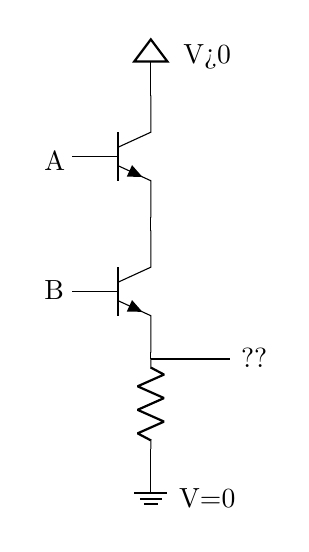
\begin{tikzpicture}
				% Paths, nodes and wires:
				\node[ground] at (1, 4.286){};
				\node[sground, yscale=-1] at (1, 9){};
				\node[shape=rectangle, minimum width=1.197cm, minimum height=0.679cm] at (1.812, 9.429){} node[anchor=north west, align=left, text width=0.809cm, inner sep=6pt] at (1.196, 9.786){V>0};
				\node[shape=rectangle, minimum width=0.608cm, minimum height=0.536cm] at (1.464, 3.857){} node[anchor=north west, align=left, text width=0.22cm, inner sep=6pt] at (1.143, 4.143){V=0};
				\node[npn] at (1, 8.143){};
				\node[npn] at (1, 6.429){};
				\draw (1, 5.571) to[american resistor, /tikz/circuitikz/bipoles/length=1.12cm] (1, 4.429);
				\draw (1, 9) -- (1, 8.913);
				\draw (1, 7.373) -- (1, 7.199);
				\draw (1, 5.659) -- (1, 5.571);
				\draw (1, 4.429) -- (1, 4.286);
				\draw (1, 5.571) -- (2, 5.571);
				\draw (0.16, 6.429) -- (0, 6.429);
				\draw (0.16, 8.143) -- (0, 8.143);
				\node[shape=rectangle, minimum width=0.679cm, minimum height=0.679cm] at (-0.214, 8.071){} node[anchor=north west, align=left, text width=0.291cm, inner sep=6pt] at (-0.571, 8.429){A};
				\node[shape=rectangle, minimum width=0.679cm, minimum height=0.679cm] at (-0.214, 6.429){} node[anchor=north west, align=left, text width=0.291cm, inner sep=6pt] at (-0.571, 6.786){B};
				\node[shape=rectangle, minimum width=0.679cm, minimum height=0.679cm] at (2.286, 5.571){} node[anchor=north west, align=left, text width=0.291cm, inner sep=6pt] at (1.929, 5.929){??};
			\end{tikzpicture}
		\end{column}
	\end{columns}
\end{frame}




\Subsection{Resistors}



\begin{frame}{What is a resistor?}
	light bulb

	ceramic

	the coils in your toaster

	something to soak up energy

	if you run electric current through it and it gets hot, it's a resistor (or at least has resistance)
\end{frame}


\begin{frame}{Voltage Drops in the Resistor}
	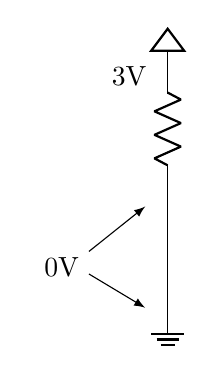
\begin{tikzpicture}
		% Paths, nodes and wires:
		\node[ground] at (2.571, 5.659){};
		\draw (2.571, 8.484) to[american resistor, /tikz/circuitikz/bipoles/length=1.12cm] (2.571, 7.199);
		\node[sground, yscale=-1] at (2.571, 8.484){};
		\node[shape=rectangle, minimum width=0.608cm, minimum height=0.536cm] at (1.964, 8.571){} node[anchor=north west, align=left, text width=0.22cm, inner sep=6pt] at (1.643, 8.857){3V};
		\node[shape=rectangle, minimum width=0.608cm, minimum height=0.536cm] at (1.107, 6.143){} node[anchor=north west, align=left, text width=0.22cm, inner sep=6pt] at (0.786, 6.429){0V};
		\draw[-latex] (1.571, 6.286) -- (2.286, 6.857);
		\draw[-latex] (1.571, 6) -- (2.286, 5.571);
		\draw (2.571, 7.199) -- (2.571, 5.659);
	\end{tikzpicture}
\end{frame}




\begin{frame}{Voltage only drops if it has somewhere to go}

Voltage drop only happens if electricity is flowing. Otherwise the voltage is the same everywhere

	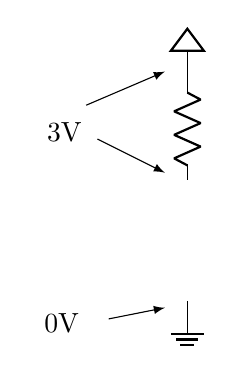
\begin{tikzpicture}
		% Paths, nodes and wires:
		\node[ground] at (2.571, 5.659){};
		\draw (2.571, 8.484) to[american resistor, /tikz/circuitikz/bipoles/length=1.12cm] (2.571, 7.199);
		\node[sground, yscale=-1] at (2.571, 8.484){};
		\node[shape=rectangle, minimum width=0.608cm, minimum height=0.536cm] at (0.893, 7.857){} node[anchor=north west, align=left, text width=0.22cm, inner sep=6pt] at (0.571, 8.143){3V};
		\node[shape=rectangle, minimum width=0.608cm, minimum height=0.536cm] at (0.857, 5.429){} node[anchor=north west, align=left, text width=0.22cm, inner sep=6pt] at (0.536, 5.714){0V};
		\draw[-latex] (1.286, 8.143) -- (2.286, 8.571);
		\draw[-latex] (1.429, 7.714) -- (2.286, 7.286);
		\draw[-latex] (1.571, 5.429) -- (2.286, 5.571);
	\end{tikzpicture}
\end{frame}


\begin{frame}{NOT ALLOWED}
	\begin{columns}
		\begin{column}{0.5\textwidth}
			We assume:
			\begin{itemize}
				\item Top rail fixed at V>0
				\item Bottom rail fixed at 0V
				\item Wires have zero resistance
			\end{itemize}
		\end{column}
		\begin{column}{0.5\textwidth}
			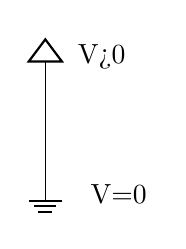
\begin{tikzpicture}
				% Paths, nodes and wires:
				\node[ground] at (1, 8){};
				\node[sground, yscale=-1] at (1, 9){};
				\node[shape=rectangle, minimum width=1.197cm, minimum height=0.679cm] at (1.813, 9.429){} node[anchor=north west, align=left, text width=0.809cm, inner sep=6pt] at (1.196, 9.786){V>0};
				\node[shape=rectangle, minimum width=0.608cm, minimum height=0.536cm] at (1.679, 7.714){} node[anchor=north west, align=left, text width=0.22cm, inner sep=6pt] at (1.357, 8){V=0};
				\draw (1, 9) -- (1, 8);
			\end{tikzpicture}		\end{column}
	\end{columns}

	If you try to build this, one of those assumptions will fail. What might that look like?

\end{frame}


\Subsection{Transistors}

\begin{frame}{Historical Transistors}
	\includegraphics[width=0.5\columnwidth]{images/tube-transistor-wiki}
\end{frame}


\begin{frame}{Modern Transistors}
	\includegraphics[width=\columnwidth]{images/semiconductor-transistor-overkill}
\end{frame}



\begin{frame}{Transistor Behavior}

	https://www.101computing.net/creating-logic-gates-using-transistors/

	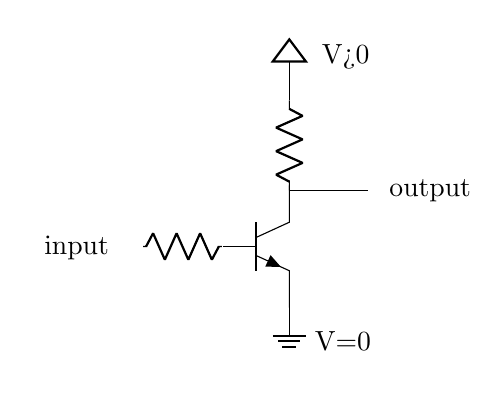
\begin{tikzpicture}
		% Paths, nodes and wires:
		\node[ground] at (1, 6.286){};
		\node[sground, yscale=-1] at (1, 9){};
		\node[shape=rectangle, minimum width=1.197cm, minimum height=0.679cm] at (1.813, 9.429){} node[anchor=north west, align=left, text width=0.809cm, inner sep=6pt] at (1.196, 9.786){V>0};
		\node[shape=rectangle, minimum width=0.608cm, minimum height=0.536cm] at (1.429, 5.857){} node[anchor=north west, align=left, text width=0.22cm, inner sep=6pt] at (1.107, 6.143){V=0};
		\draw (1, 8.857) to[american resistor, /tikz/circuitikz/bipoles/length=1.12cm] (1, 7.714);
		\draw (1, 9) -- (1, 8.857);
		\draw (1, 7.714) -- (2, 7.714);
		\node[shape=rectangle, minimum width=1.197cm, minimum height=0.679cm] at (2.67, 7.714){} node[anchor=north west, align=left, text width=0.809cm, inner sep=6pt] at (2.054, 8.071){output};
		\draw (-0.857, 7) to[american resistor, /tikz/circuitikz/bipoles/length=1.12cm] (0.143, 7);
		\draw (0.286, 7) -- (0.408, 7);
		\node[npn] at (1, 7){};
		\node[shape=rectangle, minimum width=1.197cm, minimum height=0.679cm] at (-1.714, 7){} node[anchor=north west, align=left, text width=0.809cm, inner sep=6pt] at (-2.33, 7.357){input};
	\end{tikzpicture}
\end{frame}


\begin{frame}{Transistor Behavior}
	\begin{columns}
		\begin{column}{0.5\textwidth}
			\usetikzlibrary{shapes.geometric}
			\begin{tikzpicture}
				% Paths, nodes and wires:
				\node[ground] at (1, 6.286){};
				\node[sground, yscale=-1] at (1, 9){};
				\node[shape=rectangle, minimum width=1.197cm, minimum height=0.679cm] at (1.813, 9.429){} node[anchor=north west, align=left, text width=0.809cm, inner sep=6pt] at (1.196, 9.786){V>0};
				\node[shape=rectangle, minimum width=0.608cm, minimum height=0.536cm] at (1.429, 5.857){} node[anchor=north west, align=left, text width=0.22cm, inner sep=6pt] at (1.107, 6.143){V=0};
				\draw (1, 8.857) to[american resistor, /tikz/circuitikz/bipoles/length=1.12cm] (1, 7.714);
				\node[shape=ellipse, draw, line width=1pt, dash pattern={on 1pt off 2pt}, minimum width=1.149cm, minimum height=1.108cm] at (1, 7){};
				\node[shape=rectangle, minimum width=1.197cm, minimum height=0.965cm] at (-1.33, 7.143){} node[anchor=north west, align=left, text width=0.809cm, inner sep=6pt] at (-1.946, 7.643){input\\V>0};
				\draw (1, 6.571) to[cute closed switch] (1, 7.429);
				\draw (1, 9) -- (1, 8.857);
				\draw (1, 7.714) -- (1, 7.429);
				\draw (1, 6.571) -- (1, 6.286);
				\draw (1, 7.714) -- (2, 7.714);
				\node[shape=rectangle, minimum width=1.197cm, minimum height=0.679cm] at (2.67, 7.714){} node[anchor=north west, align=left, text width=0.809cm, inner sep=6pt] at (2.054, 8.071){??};
				\draw (-0.714, 7) to[american resistor, /tikz/circuitikz/bipoles/length=1.12cm] (0.286, 7);
				\draw (0.286, 7) -- (0.408, 7);
			\end{tikzpicture}
		\end{column}
		\begin{column}{0.5\textwidth}
			\usetikzlibrary{shapes.geometric}
			\begin{tikzpicture}
				% Paths, nodes and wires:
				\node[ground] at (1, 6.286){};
				\node[sground, yscale=-1] at (1, 9){};
				\node[shape=rectangle, minimum width=1.197cm, minimum height=0.679cm] at (1.813, 9.429){} node[anchor=north west, align=left, text width=0.809cm, inner sep=6pt] at (1.196, 9.786){V>0};
				\node[shape=rectangle, minimum width=0.608cm, minimum height=0.536cm] at (1.429, 5.857){} node[anchor=north west, align=left, text width=0.22cm, inner sep=6pt] at (1.107, 6.143){V=0};
				\draw (1, 8.857) to[american resistor, /tikz/circuitikz/bipoles/length=1.12cm] (1, 7.714);
				\node[shape=ellipse, draw, line width=1pt, dash pattern={on 1pt off 2pt}, minimum width=1.149cm, minimum height=1.108cm] at (1, 7){};
				\node[shape=rectangle, minimum width=1.197cm, minimum height=0.965cm] at (-1.33, 7.143){} node[anchor=north west, align=left, text width=0.809cm, inner sep=6pt] at (-1.946, 7.643){input\\V=0};
				\draw (1, 6.571) to[cute open switch] (1, 7.429);
				\draw (1, 9) -- (1, 8.857);
				\draw (1, 7.714) -- (1, 7.429);
				\draw (1, 6.571) -- (1, 6.286);
				\draw (1, 7.714) -- (2, 7.714);
				\node[shape=rectangle, minimum width=1.197cm, minimum height=0.679cm] at (2.67, 7.714){} node[anchor=north west, align=left, text width=0.809cm, inner sep=6pt] at (2.054, 8.071){??};
				\draw (-0.714, 7) to[american resistor, /tikz/circuitikz/bipoles/length=1.12cm] (0.286, 7);
				\draw (0.286, 7) -- (0.408, 7);
			\end{tikzpicture}
		\end{column}
	\end{columns}
\end{frame}


\begin{frame}{Transistor Behavior}
	\begin{columns}
		\begin{column}{0.5\textwidth}
			\usetikzlibrary{shapes.geometric}
			\begin{tikzpicture}
				% Paths, nodes and wires:
				\node[ground] at (1, 6.286){};
				\node[sground, yscale=-1] at (1, 9){};
				\node[shape=rectangle, minimum width=1.197cm, minimum height=0.679cm] at (1.813, 9.429){} node[anchor=north west, align=left, text width=0.809cm, inner sep=6pt] at (1.196, 9.786){V>0};
				\node[shape=rectangle, minimum width=0.608cm, minimum height=0.536cm] at (1.429, 5.857){} node[anchor=north west, align=left, text width=0.22cm, inner sep=6pt] at (1.107, 6.143){V=0};
				\draw (1, 8.857) to[american resistor, /tikz/circuitikz/bipoles/length=1.12cm] (1, 7.714);
				\node[shape=ellipse, draw, line width=1pt, dash pattern={on 1pt off 2pt}, minimum width=1.149cm, minimum height=1.108cm] at (1, 7){};
				\node[shape=rectangle, minimum width=1.197cm, minimum height=0.965cm] at (-1.33, 7.143){} node[anchor=north west, align=left, text width=0.809cm, inner sep=6pt] at (-1.946, 7.643){input\\V>0};
				\draw (1, 6.571) to[cute closed switch] (1, 7.429);
				\draw (1, 9) -- (1, 8.857);
				\draw (1, 7.714) -- (1, 7.429);
				\draw (1, 6.571) -- (1, 6.286);
				\draw (1, 7.714) -- (2, 7.714);
				\node[shape=rectangle, minimum width=1.197cm, minimum height=0.679cm] at (2.67, 7.714){} node[anchor=north west, align=left, text width=0.809cm, inner sep=6pt] at (2.054, 8.071){output\\V=0};
				\draw (-0.714, 7) to[american resistor, /tikz/circuitikz/bipoles/length=1.12cm] (0.286, 7);
				\draw (0.286, 7) -- (0.408, 7);
			\end{tikzpicture}
		\end{column}
		\begin{column}{0.5\textwidth}
			\usetikzlibrary{shapes.geometric}
			\begin{tikzpicture}
				% Paths, nodes and wires:
				\node[ground] at (1, 6.286){};
				\node[sground, yscale=-1] at (1, 9){};
				\node[shape=rectangle, minimum width=1.197cm, minimum height=0.679cm] at (1.813, 9.429){} node[anchor=north west, align=left, text width=0.809cm, inner sep=6pt] at (1.196, 9.786){V>0};
				\node[shape=rectangle, minimum width=0.608cm, minimum height=0.536cm] at (1.429, 5.857){} node[anchor=north west, align=left, text width=0.22cm, inner sep=6pt] at (1.107, 6.143){V=0};
				\draw (1, 8.857) to[american resistor, /tikz/circuitikz/bipoles/length=1.12cm] (1, 7.714);
				\node[shape=ellipse, draw, line width=1pt, dash pattern={on 1pt off 2pt}, minimum width=1.149cm, minimum height=1.108cm] at (1, 7){};
				\node[shape=rectangle, minimum width=1.197cm, minimum height=0.965cm] at (-1.33, 7.143){} node[anchor=north west, align=left, text width=0.809cm, inner sep=6pt] at (-1.946, 7.643){input\\V=0};
				\draw (1, 6.571) to[cute open switch] (1, 7.429);
				\draw (1, 9) -- (1, 8.857);
				\draw (1, 7.714) -- (1, 7.429);
				\draw (1, 6.571) -- (1, 6.286);
				\draw (1, 7.714) -- (2, 7.714);
				\node[shape=rectangle, minimum width=1.197cm, minimum height=0.679cm] at (2.67, 7.714){} node[anchor=north west, align=left, text width=0.809cm, inner sep=6pt] at (2.054, 8.071){output\\V>0};
				\draw (-0.714, 7) to[american resistor, /tikz/circuitikz/bipoles/length=1.12cm] (0.286, 7);
				\draw (0.286, 7) -- (0.408, 7);
			\end{tikzpicture}
		\end{column}
	\end{columns}
\end{frame}



\begin{frame}{Why two resistors?}

In many cases, we can get away with just one resistor. The previous example had two. Why?

Always need a resistor between a voltage source and ground. Transistors have internal resistance but it's very small. Easy to burn them out

\end{frame}





\begin{frame}{More Complex Example}
	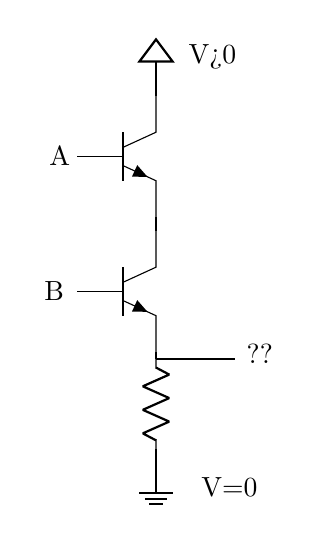
\begin{tikzpicture}
		% Paths, nodes and wires:
		\node[ground] at (1, 4.286){};
		\node[sground, yscale=-1] at (1, 9){};
		\node[shape=rectangle, minimum width=1.197cm, minimum height=0.679cm] at (1.813, 9.429){} node[anchor=north west, align=left, text width=0.809cm, inner sep=6pt] at (1.196, 9.786){V>0};
		\node[shape=rectangle, minimum width=0.608cm, minimum height=0.536cm] at (1.679, 4){} node[anchor=north west, align=left, text width=0.22cm, inner sep=6pt] at (1.357, 4.286){V=0};
		\draw (1, 5.571) to[american resistor, /tikz/circuitikz/bipoles/length=1.12cm] (1, 4.429);
		\node[npn] at (1, 8.143){};
		\node[npn] at (1, 6.429){};
		\draw (1, 9) -- (1, 8.913);
		\draw (1, 7.373) -- (1, 7.199);
		\draw (1, 5.659) -- (1, 5.571);
		\draw (1, 5.571) -- (2, 5.571);
		\draw (0.16, 8.143) -- (0, 8.143);
		\draw (0.16, 6.429) -- (0, 6.429);
		\draw (1, 4.429) -- (1, 4.286);
		\node[shape=rectangle, minimum width=0.668cm, minimum height=0.65cm] at (-0.22, 8.143){} node[anchor=north west, align=left, text width=0.28cm, inner sep=6pt] at (-0.571, 8.485){A};
		\node[shape=rectangle, minimum width=0.668cm, minimum height=0.65cm] at (-0.286, 6.429){} node[anchor=north west, align=left, text width=0.28cm, inner sep=6pt] at (-0.637, 6.771){B};
		\node[shape=rectangle, minimum width=0.668cm, minimum height=0.65cm] at (2.286, 5.628){} node[anchor=north west, align=left, text width=0.28cm, inner sep=6pt] at (1.934, 5.971){??};
	\end{tikzpicture}
\end{frame}




% what is a transistor
% building logic gates

% TEST 3 TOPICS

\Section{Instruction Pipelining}

\Subsection{FDEW Cycle}

\Subsection{Pipelining}

\Subsection{Hazards}

% pipelining
% data hazards
% control hazards

\Section{Assembly Conditionals and Loops}

% b, beq, bne, ...
% if/else
% while loops
% for loops

\input{sections/multiprocessing.tex}
% booting
% forking
% threads, cores, processes
% async


\Section{Appendix}


\Subsection{Raspberry Pi Setup}


\begin{frame}{Pi Setup: Kit Contents}
	\begin{columns}
		\begin{column}{0.5\textwidth}
			\begin{enumerate}
				\item Pi case
				\item Raspberry Pi (in box)
				\item Heat sinks
				\item Power cord
				\item Ethernet to USB adapter
				\item Ethernet cord
				\item USB 2 to USB 3 adapter
				\item SD Card
				\item Accessory case
			\end{enumerate}
		\end{column}
		\begin{column}{0.5\textwidth}
			\includegraphics[width=\columnwidth]{images/pi-kit-contents}
		\end{column}
	\end{columns}
\end{frame}


\begin{frame}{Pi Setup: Apply Heat Sinks}
	\begin{columns}
		\begin{column}{0.5\textwidth}
			\includegraphics[width=\columnwidth]{images/pi-heat-sinks-1}
		\end{column}
		\begin{column}{0.5\textwidth}
			\includegraphics[width=\columnwidth]{images/pi-heat-sinks-2}
		\end{column}
	\end{columns}
\end{frame}

\begin{frame}{Pi Setup: Apply Nonslip Nubs}
	\includegraphics[width=\columnwidth]{images/pi-case-nubs}
\end{frame}

\begin{frame}{Pi Setup: Install in Case}
	\includegraphics[width=\columnwidth]{images/pi-in-case}
\end{frame}

\begin{frame}{Pi Setup: SD Card}
	\begin{columns}
		\begin{column}{0.5\textwidth}
			\includegraphics[width=\columnwidth]{images/pi-sd-card-1}
		\end{column}
		\begin{column}{0.5\textwidth}
			\includegraphics[width=\columnwidth]{images/pi-sd-card-2}
		\end{column}
	\end{columns}
\end{frame}

\begin{frame}{Pi Setup: Connect to Laptop}
	\includegraphics[width=\columnwidth]{images/pi-to-laptop}
\end{frame}

\begin{frame}{Pi Setup: Connect to Power}
\end{frame}

\begin{frame}{Laptop Setup: Enable WiFi}
	\includegraphics[width=\columnwidth]{images/pi-network-settings}
\end{frame}

\begin{frame}{Laptop Setup: Install VSCode}
	\includegraphics[width=\columnwidth]{images/vscode-remote-ssh}
\end{frame}

\begin{frame}{Laptop Setup: Add Remote Connection}
	\includegraphics[width=\columnwidth]{images/vscode-add-remote}
\end{frame}

\begin{frame}{Laptop Setup: SSH Login}
	\begin{itemize}
		\item Default username/password is raspberri/pi
		\item Make sure to update username and password
	\end{itemize}
\end{frame}


\Subsection{CSGit Setup}

% vscode setup
% pi setup
% csgit setup


\end{document}
% parts of a computer
% memory hierarchy
% executing instructions
% the von neumann bottleneck
% clock-driven execution
% instruction walkthrough
% pipelining
% data hazards
% control hazards


\documentclass{beamer}
\usepackage[utf8]{inputenc}
\usepackage[T1]{fontenc}
\usepackage{circuitikz}

\usepackage{multirow}

\title{CS241: Hardware Design}
\date{\today}
\author[Fyfe and Lynn]{Charles Fyfe and Melissa Lynn}
\institute{St Olaf College}

\usetheme{grape}

\usepackage{parskip}
\usepackage{multicol}
\usepackage{graphicx}
% make \oplus look nice
\usepackage{amssymb}

\begin{document}


\titlepage

% just sections up top
\setcounter{tocdepth}{1}

\begin{frame}{Outline}

	\begin{multicols*}{2}
		\tableofcontents
	\end{multicols*}
\end{frame}

% show subsections later
\setcounter{tocdepth}{2}


\Section{Syllabus}

\begin{frame}{Course Overview}

	\includegraphics[width=\columnwidth]{images/dune-robot-hbo}

	{\center
		Thou shalt not make a machine in the likeless of a human mind
	}

	{\small \hfill
		The Orange Catholic Bible, Dune, Frank Herbert
	}
\end{frame}


\begin{frame}{Course Overview}

	Computers feel like magic. You type words. The machine does complex things. Especially in the era of large language models

	But it's not magic. Computers are made of semiconductors, metal, and magnets. Three different kinds of rocks

	This course is about demystifying the machine and exploring how, fundamentally, computers do what they do. Specifically, we'll be looking at:
	\begin{itemize}
		\item The fundamental components of a computer
		\item How data is stored on a computer
		\item Building electrical circuits to perform logic
		\item Programming in Assembly (a very low-level language)
	\end{itemize}
\end{frame}

\Subsection{Grading}

\begin{frame}{Course Grade Breakdown}
	\begin{itemize}
		\item Quizzes and final: 45\%
		\item Homework and labs: 45\%
		\item Participation: 10\%
	\end{itemize}
\end{frame}

\begin{frame}{Standards-Based Grading}
	\begin{itemize}
		\item There are nine standards in the class. Each is worth 5\% of your grade.
		\item There are three quizzes. Each quiz covers three standards.
		\item The final covers all nine standards.
		\item If you demonstrate proficiency on the quiz, you're done with that standard. Full credit. You can skip that part of the final.
		\item If you demonstrate partial proficiency on the quiz, you get half credit. Try again on the final for full credit.
		\item If you do not demonstrate proficiency on the quiz, you get no credit. You can still get full credit on the final!
	\end{itemize}
\end{frame}


\begin{frame}{Homework and Labs}
	\begin{itemize}
		\item One or more lab exercises for each standard. We start these together in class. You may need to finish on your own time.
		\item We will have a homework assignment for each standard.
		\item Please work together in small groups.
		\item Please ensure that the work you turn in reflects your own understanding.
	\end{itemize}
\end{frame}

\begin{frame}{Late Work Policy}
	Please try to get your work in on time.
	\begin{itemize}
		\item If you don't get your work done on time, you may fall behind in the class.
		\item Late work is inconvenient for the TAs. They will be grumpy and vindictive when they grade your work.
		\item TAs will have their own finals to worry about! Late work at the end of the semester might be refused.
	\end{itemize}
	If you need an extension, please reach out beforehand.
\end{frame}

\begin{frame}{Peer Reviews}
	\begin{itemize}
		\item Participation score (10\% of your total grade) is mostly based on peer reviews.
		\item Reviews will be short. Less than one page.
		\item You can get full credit here without too much trouble. Show up. Work together. Make it easy for your peers to say nice things about you.
		\item I recommend keeping notes over the course of the semester when someone is particularly helpful, insightful, etc. Good reviews have concrete examples.
	\end{itemize}
\end{frame}

\Subsection{Office Hours}

\begin{frame}{Office Hours}
	TODO
\end{frame}


\Subsection{Disability Accommodations}

\begin{frame}{Disability Accommodations}
	I am committed to supporting the learning of all students in my class. If you have already
	registered with Disability and Access (DAC) and have your letter of accommodations, please
	meet with me as soon as possible to discuss, plan, and implement your accommodations in the
	course. If you have or think you have a disability (learning, sensory, physical, chronic health,
	mental health or attentional), please contact Disability and Access staff at 507-786-3288 or by visiting \href{https://wp.stolaf.edu/academic-support/dac}{their website}.


	If you have an accommodation that allows you extra time or a low distraction environment for
	quizzes and exams, please email me at least three days before each quiz or exam, so that I can
	make sure to reserve a room.
\end{frame}


\Subsection{Religious Accommodations}

\begin{frame}{Religious Accommodations}
	As part of my commitment to make St Olaf an inclusive community, I will provide students with
	reasonable religious accommodations. If you will be missing class for a religious observance or
	require another religious accommodation, please meet with me to discuss these.
\end{frame}


\Subsection{Academic Integrity}

\begin{frame}{Academic Integrity}

	Plagiarism is a serious academic offense. Hand in your own work. Give credit appropriately when you draw from the work of others. For more information please see:

	\begin{itemize}
		\item \href{https://wp.stolaf.edu/facultyhandbook/academic-integrity-faculty-handbook-category-2}{Faculty Handbook: Academic Integrity}
		\item \href{https://wp.stolaf.edu/honorcouncil/}{The Honor Code}
		\item \href{https://wp.stolaf.edu/roadmap-to-academic-integrity}{Roadmap to Academic Integrity}
	\end{itemize}

	Work that violates this policy will typically receive no credit. In especially serious cases the penalty can be an F in the course.
\end{frame}

\Subsection{AI Use Policy}

\begin{frame}{AI Usage Policy}
	Please not submit AI work as your own.

	You may use AI tools when studying, but be careful. These tools are very good with mainstream languages like Python. We're working with Assembly, which is very much \textbf{not} a mainstream language.

\end{frame}


\Subsection{St Olaf Land Acknowledgement}

\begin{frame}{St Olaf Land Acknowledgement}
	We stand on the homelands of the Wahpekute Band of the Dakota Nation. We honor with
	gratitude the people who have stewarded the land throughout the generations and their ongoing
	contributions to this region. We acknowledge the ongoing injustices that we have committed
	against the Dakota Nation, and we wish to interrupt this legacy, beginning with acts of healing
	and honest storytelling about this place.

	For more information about land acknowledgement statements at St Olaf, please see \href{https://wp.stolaf.edu/education/land-acknowledgement/}{here} and \href{https://wp.stolaf.edu/equity-inclusion/land-acknowledgement/}{here}.
\end{frame}


\Subsection{Statement of Inclusivity}

\begin{frame}{Statement of Inclusivity}
	In keeping with St. Olaf College's mission statement, this class strives to be an inclusive
	learning community, respecting those of differing backgrounds and beliefs. As a community, we
	aim to be respectful to all citizens in this class, regardless of race, ethnicity, religion, gender or
	sexual orientation.
\end{frame}


\Subsection{Gender Pronouns}

\begin{frame}{Gender Pronouns}
	This course affirms people of all gender expressions and gender identities. If you go by a
	different name than what is on the class roster, please let me know.

	Using correct gender
	pronouns is important to me, so you are encouraged to share your pronouns with me and
	correct me if a mistake is made. If you have any questions or concerns, please do not hesitate
	to contact me.
\end{frame}


\Subsection{Multilingual Student Support}

\begin{frame}{Multilingual Student Support}
	I am committed to making course content accessible to all students. If English is not your first
	language and this causes you concern about the course, please speak with me. Students who
	would like extra support with writing or speaking in English can also contact the language support specialist (\href{mailto:berryag@stolaf.edu}{berryag@stolaf.edu}) in the Academic Success Center.
\end{frame}


\Subsection{Mental Health}

\begin{frame}{Mental Health}

	I greatly value your experience in this class, and it is my duty to facilitate a safe, caring, and
	productive learning environment.

	I recognize that you may experience a range of emotional, physical, and/or psychological
	issues, both in and out of the classroom, that may distract you from your learning.

	If you are experiencing such issues, please do not hesitate to come see me. I am here to listen.
	We can also discuss what further resources might be available to you.
\end{frame}

\Subsection{Required Referrals}


\begin{frame}{Required Referrals}
	You are welcome to talk to me about circumstances outside the course that
	affect your classroom experience or acadmic performance. However, please keep
	in mind that I am required to refer cases of discrimination, harassment,
	sexual misconduct, and violence.

	Here are some resources where you can share privately:

	\begin{itemize}
		\item Boe House Counseling Center
		\item College Pastors and Chaplains
		\item Sexual Assault Resource Network (SARN)
		\item Health Services
		\item TimelyCare
	\end{itemize}
\end{frame}




\Subsection{St. Olaf Pride Statement}

\begin{frame}{St. Olaf Pride Statement}
	As an Ole, I will practice:
	\begin{itemize}
		\item Passion for learning and pursuit of vocation
		\item Respect for the worth and dignity of all people
		\item Integrity at all times, in all circumstances
		\item Dedication to a life of service, and
		\item Engagement with my community and the world.
	\end{itemize}
\end{frame}









\Subsection{Important Links}

\begin{frame}{Important Links}
	\begin{itemize}
		\item ARM tutorial https://computerscience.chemeketa.edu/armTutorial/index.html
		\item ARM simulator https://cpulator.01xz.net/?sys=arm
		\item circuit simulator: https://circuitverse.org/simulator
	\end{itemize}
\end{frame}





% TEST 1 TOPICS


\Section{Data Representation}

\begin{frame}{How do computers store information?}
	Computers work using electrical signals which can be on or off. If we let:
	\begin{itemize}
		\item On means 1
		\item Off means 0
	\end{itemize}
	We can use sequences of 0s and 1s to represent information
\end{frame}

\Subsection{Positive Integers in Binary}

\begin{frame}{Numbers in Base Ten (aka Decimal)}
	Let's start by talking about how we write numbers normally.

	For example, let's look at the number 109:
	\begin{align*}
		109 & = 100 \;+\; 0 \;+\; 9                                   \\
		    & = 1 \Times 10^2 \;+\; 0 \Times 10^1 \;+\; 9 \Times 10^0
	\end{align*}
	This way of writing numbers is called base ten.
	We use ten digits (0 to 9 inclusive) and each position in the number is scaled by a power of ten.

	In terms of math, there is nothing special about base ten. We probably use it
	because we have ten fingers. Some ancient civilizations used sompletely
	different systems for counting!
\end{frame}

\begin{frame}{Numbers in Base Two (aka Binary)}
	Computers don't have fingers. They express everything as sequences of 1s and 0s. This format is called binary:

	\begin{align*}
		0b1101101 & =
		1 \Times 2^6 +
		1 \Times 2^5 +
		0 \Times 2^4 +
		1 \Times 2^3 +
		1 \Times 2^2 +
		0 \Times 2^1 +
		1 \Times 2^0                              \\
		          & = 64 + 32 + 0 + 8 + 4 + 0 + 1 \\
		          & = 109                         \\
	\end{align*}
	Importantly: we always use the prefix ``0b'' to avoid confusion when writing numbers in binary.

	1101 is one thousand one hundred and one

	0b1101 is thirteen
\end{frame}

\begin{frame}{Converting from Decimal to Binary}

	If the number is odd, append a 1 on the left. Otherwise, append a 0. Then
	divide your decimal number by two and ignore any remainder. Repeat until your
	decimal number is zero. \\

	For example, starting with 58:

	\begin{itemize}
		\item 58 is even, so append \Highlight{0}. Divide by two, leaving 29.
		\item 29 is odd, so append \Highlight{1}0. Divide by two, leaving 14.
		\item 14 is even, so append \Highlight{0}10. Divide by two, leaving 7.
		\item 7 is odd, so append \Highlight{1}010. Divide by two, leaving 3.
		\item 3 is odd, so append \Highlight{1}1010. Divide by two, leaving 1.
		\item 1 is odd, so append \Highlight{1}11010. Divide by two, leaving 0.
	\end{itemize}

	So 58 in binary is 0b111010.

\end{frame}

\begin{frame}{Converting from Binary to Decimal}

	We can confirm by converting back. The rightmost bit is worth 1, then 2, then
	4, and so on:

	\begin{align*}
		0b111010 & =
		1 \Times 2^5 +
		1 \Times 2^4 +
		1 \Times 2^3 +
		0 \Times 2^2 +
		1 \Times 2^1 +
		0 \Times 2^0                          \\
		         & = 32 + 16  + 8 + 0 + 2 + 0 \\
		         & = 58
	\end{align*}

\end{frame}

\begin{frame}{Addition in Binary}
	Binary addition works just like decimal addition.
	Start from the right, add straight down, and carry when you run out of digits.

	For example:
	\[
		\begin{array}{ccccccccc}
			1 & 1 & 1 & 1 & 1 &   &   &   &   \\
			  & 0 & 0 & 1 & 1 & 1 & 0 & 0 & 0 \\
			+ & 1 & 1 & 1 & 0 & 1 & 0 & 0 & 1 \\
			\hline
			1 & 0 & 0 & 1 & 0 & 0 & 0 & 0 & 1 \\
		\end{array}
	\]

	What happens if we try to perform this operation but we only have 8 bits to
	store the answer?
\end{frame}

\begin{frame}{Multiplication in Binary}
	Binary multiplication works just like decimal multiplication.
	Multiply the top number by the rightmost digit of the bottom number.
	Then move to the next line, add a zero, and repeat for the next digit.
	Finally, add up the lines. For example:
	\[
		\begin{array}{cccccc}
			  &   &        & 1 & 1 & 0 \\
			  &   & \times & 1 & 0 & 1 \\
			\hline
			  &   &        & 1 & 1 & 0 \\
			  &   & 0      & 0 & 0 & 0 \\
			+ & 1 & 1      & 0 & 0 & 0 \\
			\hline
			  & 1 & 1      & 1 & 1 & 0 \\
		\end{array}
	\]
\end{frame}

\begin{frame}{Division in Binary}
	To divide by 2, shift the bits one place to the right. \\

	To divide by 4, shift the bits two places to the right. \\

	That's about as deep as we go in this class. If you're curious to learn more,
	see the textbook.

\end{frame}



\Subsection{Hexadecimal}

\begin{frame}{What? Why?}

	Binary is how machines store data. But writing out binary by hand is a chore.
	In practice, it's often convenient to use hexadecimal (base 16) instead.

	\begin{itemize}
		\item Decimal uses ten digits, 0-9
		\item Binary uses two digits, 0 and 1
		\item Hexadecimal uses sixteen digits: 0-9 along with A-F
	\end{itemize}
	Hexadecimal values are always prefixed with ``0x'' to avoid ambiguity.
\end{frame}

\begin{frame}{Converting Between Binary and Hexadecimal}

	Converting back and forth between binary and hexadecimal does not require any
	math! Every four bits become one hex digit.
	\begin{align*}
		0b0000 & = 0x0 = 0 & 0b1000 & = 0x8 = 8  \\
		0b0001 & = 0x1 = 1 & 0b1001 & = 0x9 = 9  \\
		0b0010 & = 0x2 = 2 & 0b1010 & = 0xA = 10 \\
		0b0011 & = 0x3 = 3 & 0b1011 & = 0xB = 11 \\
		0b0100 & = 0x4 = 4 & 0b1100 & = 0xC = 12 \\
		0b0101 & = 0x5 = 5 & 0b1101 & = 0xD = 13 \\
		0b0110 & = 0x6 = 6 & 0b1110 & = 0xE = 14 \\
		0b0111 & = 0x7 = 7 & 0b1111 & = 0xF = 15 \\
	\end{align*}
\end{frame}

\begin{frame}{Converting Hexadecimal to Decimal}

	Hexadecimal is base 16. So each place corresponds to a power of 16.

	\begin{align*}
		0x3AB & = 3 \times 16^2 + 10 \times 16^1 + 11 \times 16^0 \\
		      & = 3 \times 256 + 10 \times 16 + 11 \times 1       \\
		      & = 768 + 160 + 11                                  \\
		      & = 954                                             \\
	\end{align*}

	Hexadecimal is very compact! These numbers get big fast

\end{frame}

\begin{frame}{Arithmetic in Hexadecimal}

	Addition and multiplication work in hexadecimal just like they do in binary and
	decimal. Just be careful about carrying.

	\[
		\begin{array}{ccccc}
			1 &   &   & 1 &   \\
			  & 4 & 1 & 7 & B \\
			+ & C & 2 & 0 & F \\
			\hline
			1 & 0 & 3 & 8 & A \\
		\end{array}
	\]

\end{frame}






\Subsection{Negatives in Binary}

\begin{frame}{First Attempt: Signed Magnitude}

	We can use the first digit to hold the sign, then the rest of the digits to
	hold magnitue:

	\begin{itemize}
		\item 0b\Highlight{0}1011001 is positive 10110001, so 89
		\item 0b\Highlight{1}1011001 is negative 1011001, so -89
	\end{itemize}

	This is nice and straightforward!

\end{frame}

\begin{frame}{Addition and Subtraction with Signed Magnitude}
	Adding positive numbers works just the same. But what happens if we throw a minus sign in there?

	For example, let's look at 12 - 5. First, rewrite it as 12 + (-5). Then:

	\[
		\begin{array}{ccccccccc}
			  & 0 & 0 & 0 & 0 & 1 & 1 & 0 & 0 \\
			+ & 1 & 0 & 0 & 0 & 0 & 1 & 0 & 1 \\
			\hline
			  & ? & ? & ? & ? & ? & ? & ? & ? \\
		\end{array}
	\]

	We know the result should be 7 (0b00000111). But our regular rules for addition
	do not get us there.
\end{frame}

\begin{frame}{Zero with Signed Magnitude}

	Using signed magnitude, 0b00000000 is zero.

	And 0b10000000 is negative zero (which is also zero).

	Using this convention, we have to worry about the difference between numerical
	equality and bitwise equality. That seems pretty messy.
\end{frame}

\begin{frame}{Can We Do Better?}
	Signed magnitude was a swing and a miss. What do we want when we talk about negative numbers?
	\begin{itemize}
		\item We want positive numbers to work like we expect
		\item We want 0b00000000 to be zero, with no ambiguity
		\item We want addition and subtraction to work the same for positive and negative
	\end{itemize}
\end{frame}

\begin{frame}{Another Idea: Two's Complement}
	We know 1 - 1 = 0. Put another way, 1 + (-1) = 0. Can we work backwards from there to figure out how to write -1?
	\[
		\begin{array}{ccccccccc}
			  & 0 & 0 & 0 & 0 & 0 & 0 & 0 & 1 \\
			+ & 1 & 1 & 1 & 1 & 1 & 1 & 1 & 1 \\
			\hline
			  & 0 & 0 & 0 & 0 & 0 & 0 & 0 & 0 \\
		\end{array}
	\]

	Remember: on a computer, our numbers have to fit in a set number of bits.
	Anything past that gets thrown away. This is called overflow. In this case,
	overflow works in our favor!
\end{frame}

\begin{frame}{Working Backwards from Zero}
	We can use the same trick to identify the rest of the negative numbers:
	\begin{itemize}
		\item 0b00000000 is 0
		\item 0b11111111 is -1
		\item 0b11111110 is -2
		\item 0b11111101 is -3
		\item 0b11111100 is -4
		\item etc
	\end{itemize}

\end{frame}

\begin{frame}{The Sign Bit (Again)}
	We only have 256 possible integers. How do we decide where the positives end and the negatives begin?

	Unsigned int: bits are worth 1, 2, 4, 8, 16, 32, 64, 128

	Signed magnitude: bits are worth $\pm1, \pm2, \pm4, \pm8, \pm16, \pm32, \pm64$,
	and the last bit tells us whether to use positive or negative (yikes)

	Two's complement: bits are worth 1, 2, 4, 8, 16, 32, 64, \Highlight{-128}

	Range of possible values is -128 to 127.
\end{frame}

\begin{frame}{Flipping Signs in Two's Complement}
	To flip the sign of a two's complement integer, flip all the bits then add 1. Ignore the overflow (if any). This works for both positive and negative numbers.

	For example:
	\begin{itemize}
		\item 55 is 0b01010111
		\item Flip the bits: 0b10101000, then add 1: 0b10101001
		\item So -55 is 0b10101001
		\item Flip the bits again: 0b01010110, add 1: 0b01010111
		\item So -(-55) = 55 = 0b01010111
	\end{itemize}

	What happens if we negate zero?
\end{frame}

\begin{frame}{Overflow}
	Overflow is important for two's complement. It ensures that positive zero and negative zero are the same. But it is also a constraint!

	Try adding 0b01101001 + 0b01011010:
	\[
		\begin{array}{ccccccccc}
			  &   & 1 & 1 & 1 &   &   &   &   \\
			  & 0 & 1 & 1 & 0 & 1 & 0 & 0 & 1 \\
			+ & 0 & 1 & 0 & 1 & 1 & 0 & 1 & 0 \\
			\hline
			  & 1 & 1 & 0 & 0 & 0 & 0 & 1 & 1 \\
		\end{array}
	\]

	These are two's complement numbers. Convert them to decimal. What just
	happened?

\end{frame}


\Subsection{Fractions and Decimals}

\begin{frame}{The Decimal Point}

	Sometimes we need to store numbers that aren't integers. \\

	Before we worry about binary, what does 21.867 mean? \\

	\begin{align*}
		21.867 & = 2 \Times 10^1 + 1 \Times 10^0 + 8 \Times ?? + 6 \Times ?? + 7 \Times ??
	\end{align*}

\end{frame}

\begin{frame}{The Decimal Point}

	In decimal:
	\begin{align*}
		21.867 & = 2 \Times 10^1 + 1 \Times 10^0 + 8 \Times 10^{-1} + 6 \Times 10^{-2} + 7 \Times 10^{-3}             \\
		       & =2 \Times 10 + 1 \Times 1 + 8 \Times \frac{1}{10} + 6 \Times \frac{1}{100} + 7 \Times \frac{1}{1000} \\
	\end{align*}

	In binary, we can use the same idea:
	\begin{align*}
		0b101.010 & = 1 \Times 2^2 + 0 \Times 2^1 + 1 \Times 2^0 + 0 \Times 2^{-1} + 1 \Times 2^{-2} + 0 \Times 2^{-3} \\
		          & = 1 \Times 4 + 0 + 1 \Times 1 + 0 + 1 \Times \frac{1}{4} + 0                                       \\
		          & = 5.25                                                                                             \\
	\end{align*}

\end{frame}

\begin{frame}{Fixed Point Representation}

	The computer just stores 1s and 0s, not decimal points. How do we distinguish
	these values?
	\begin{itemize}
		\item 0b0101110.1 = 46.5
		\item 0b010111.01 = 23.25
		\item 0b01011.101 = 11.625
	\end{itemize}

	One option is to specify the location of the decimal point ahead of time. For
	example, we could say that our eight-bit binary decimal always has two decimal
	bits. \\

	What is an upside of this approach? What is a downside?

\end{frame}

\begin{frame}{Floating Point Representation}

	Floating point numbers are a bit more complicated, but much more flexible. For
	a 16-bit floating point number we get:

	\begin{itemize}
		\item 1 bit for the sign
		\item 5 bits for the exponent (value -14 to 15)
		\item 10 bits for the significand (value 0 to 1023)
	\end{itemize}

	To turn those components into a value we use:
	\begin{align*}
		\text{value} & = (-1)^{\text{sign}} \times 2^{\text{exponent} - 15} \times \left(1 + \frac{\text{significand}}{1024} \right)
	\end{align*}

	Why offset the exponent?

	Why add 1 to the significand fraction?

\end{frame}

% Explanation here for the 127 offset: https://www.quora.com/Why-do-we-add-127-to-the-exponent-in-IEEE-754-floating-number-format-to-get-the-actual-exponent-value

\begin{frame}{Floating Point Examples}

	\begin{align*}
		\underbrace{0}_\text{sign} \; \underbrace{01111}_\text{exponent} \; \underbrace{0000000000}_\text{significand} & = (-1)^0 \times 2^{15 - 15} \times \left( 1 + \frac{0}{1024} \right) \\
		                                                                                                               & = 1 \times 2^0   \times \left( 1 + 0 \right)                         \\
		                                                                                                               & = 1                                                                  \\
	\end{align*}
	\begin{align*}
		0 \; 01101 \; 0101010101 & = (-1)^0 \times 2^{13 - 15} \times \left( 1 + \frac{341}{1024} \right) \\
		                         & \approx 0.33325195                                                     \\
	\end{align*}
	\begin{align*}
		1 \; 11110 \; 1111111111 & = (-1)^1 \times 2^{30 - 15} \times \left( 1 + \frac{1023}{1024} \right) \\
		                         & = -65504                                                                \\
	\end{align*}

	Why
\end{frame}

\begin{frame}{Floating Point Special Cases}

	\[
		\begin{array}{ccccr}
			0 & 00000 & 0000000000     & = 0          \\
			1 & 00000 & 0000000000     & = -0         \\
			0 & 11111 & 0000000000     & = \infty     \\
			1 & 11111 & 0000000000     & = -\infty    \\
			0 & 11111 & \text{nonzero} & = \text{NaN} \\
		\end{array}
	\]

	There's more to it than this. If you're curious, read up on subnormal numbers
	\href{https://en.wikipedia.org/wiki/Half-precision_floating-point_format}{here}

\end{frame}

\begin{frame}{Floating Point for Big Integers}

	If we're dealing with big numbers, floating point often works better than fixed
	point. This is true even if both formats use the same number of bits.

	\begin{itemize}
		\item 8-bit unsigned integer: max value 255
		\item 16-bit unsigned integer: max value 65,535
		\item 32-bit unsigned integer: max value 4.2 billion % 4,294,967,295
		\item 16-bit floating point: max value 65,504 (also handles negatives, fractions)
		\item 32-bit floating point: max value 340 billion billion billion billion (also handles negatives, fractions)
		      % 340,282,346,638,528,859,811,704,183,484,516,925,440 
	\end{itemize}

\end{frame}

\begin{frame}{Floating Point Limitations}

	So what's the catch?

\end{frame}

%        \item Convert 0b100110.10 from fixed-point binary to decimal.
%        \item Convert 23.75 from decimal to fixed-point binary.
%        \item Add fixed-point binary numbers 0b101101.01 + 0b010011.11. Convert to decimal to confirm your result.
%        \item Show that the 16-bit floating point expression ${1 \; 01000 \; 1100000000}$ is equal to -3.5 in decimal.

\Subsection{Beyond Numbers}

\begin{frame}{What else do computers store?}
	There are many cases where we want a computer to store non-numerical data:
	\begin{itemize}
		\item Text
		\item Colors
		\item Sounds
		\item Images
		\item Videos
		\item Websites
		\item Multiple things at once
	\end{itemize}
\end{frame}

\begin{frame}{Characters and Strings}
	\begin{itemize}
		\item Each character is represented by a number
		\item The most straightforward encoding is ASCII
		\item Modern use cases typically use Unicode (much bigger)
		\item To make a string, put a bunch of characters in a row
		\item Question: how do we identify the end of a string?
	\end{itemize}
\end{frame}

\begin{frame}{ASCII Table}
	\includegraphics[width=\columnwidth]{images/ascii-table}
\end{frame}

\begin{frame}{Colors and Images}
	\begin{itemize}
		\item A color can be described by three numbers (R, G, B)
		\item We can represent an image as a grid of colored pixels
		\item Question: do we need a null byte at the end of a pixel/row/image? Why or why not?
	\end{itemize}
	\includegraphics[width=\columnwidth]{images/mario-pixels}
\end{frame}

\begin{frame}{Sound}
	\begin{itemize}
		\item Sound is pressure vibrations in the air
		\item We can create sound by moving a speaker cone rapidly
		\item To store sound, store the movement of the speaker cone
	\end{itemize}
	\includegraphics[width=0.5\columnwidth]{images/speakers}
\end{frame}

\begin{frame}{Structured Data}
	\begin{itemize}
		\item When you go to a website, how does your browser know what to display?
		\item When you add an item to your online cart, what data is sent?
	\end{itemize}
	\begin{columns}
		\begin{column}{0.5\textwidth}
			\includegraphics[width=\columnwidth]{images/html-example}
		\end{column}
		\begin{column}{0.5\textwidth}
			\includegraphics[width=\columnwidth]{images/json-example}
		\end{column}
	\end{columns}
\end{frame}









% positive integers in binary
% arithmetic in binary
% negtive integers
% hex
% fractions
% structured data

\input{sections/02-boolean-logic.tex}
% boolean operators
% boolean expressions
% boolean circuits

\Section{Assembly Globals}

\begin{frame}{Coding in Assembly}

	You'll be doing coding exercises on an online emulator, as well as on your Raspberry Pi

\end{frame}

\Subsection{Why study assembly?}

\begin{frame}[fragile]{Hello World in C}
	\begin{minted}{C}
		#include <stdio.h>

		int main() {
			printf("Hello world!\n");
			return 0;
		}
	\end{minted}

	Your local C compiler can turn this into an executable, which you can then run:

	\begin{minted}{bash}
		$ gcc hello.c
		$ ./a.out
		Hello world!
	\end{minted}
\end{frame}


\begin{frame}[fragile]{Hello World in Python}
	\begin{minted}{python}
		print('Hello world!')
	\end{minted}

	You can run this using your local Python interpreter:
	\begin{minted}{bash}
		$ python3 hello.py
		Hello world!
	\end{minted}
\end{frame}

\begin{frame}[fragile]{Hello World in Assembly}
	% haven't yet found a perfect highlighter match
	% tasm - dislikes pound signs for int literals
	% nasm, gas - dislikes comments with @
	% ca65 - comments and a lot of commands all black
	% llvm, dasm16, hsail - nope
	% hsail
	\begin{minted}{tasm}
		.section .rodata
		greeting: .ascii "Hello world!\n\0"

		.section .text
		.global _start
		_start:
		ldr r0, =greeting
		bl printf
		mov r0, #0
		bl exit
	\end{minted}

	You can assemble this into an executable and run it on your Raspberry Pi:
	\begin{minted}{bash}
		$ gcc hello.s
		$ ./a.out
		Hello world!
	\end{minted}
\end{frame}

\begin{frame}{What makes assembly special?}
	\begin{itemize}
		\item It takes a lot of lines to do anything
		\item There is so much boilerplates
		\item Yikes
	\end{itemize}
\end{frame}

\begin{frame}{What makes assembly special?}
	\begin{itemize}
		\item Every computer architecture is a little bit different. An Intel CPU and an AMD CPU can both run the same logic, but they will do things in slightly different ways.
		\item When coding in C, you (mostly) don't have to worry about it. The compiler figures out how to make your logic work on the current hardware.
		\item Same for Python. The interpreter (written in C and compiled) figures out how to make your logic work on the current hardware.
		\item Assembly is not like that. Intel assembly is tied to the hardware specifics of the Intel CPU. ARM assembly is a different language.
		\item We study assembly because we want to talk about what is happening on hardware.
	\end{itemize}

	%	The following command compiles a program in C:
	%	\begin{minted}{bash}
	%		gcc hello.c -o hello
	%	\end{minted}
	%	This creates several intermediate files, eventually creating an executable file (which we can run).
	%	`hello.c' -> preprocessor -> `hello.i' -> compiler -> `hello.s' -> assembler -> `hello.o' -> linker -> `hello'

\end{frame}

% per wikipedia:
% Each computer architecture has its own machine language. Computers differ in the number and type of operations they support, in the different sizes and numbers of registers, and in the representations of data in storage. While most general-purpose computers are able to carry out essentially the same functionality, the ways they do so differ; the corresponding assembly languages reflect these differences.

\Subsection{Global Constants}

\begin{frame}{Global Constants}
	\begin{itemize}
		\item A global constant is defined in the code
		\item Its value does not change during runtime
		\item It has a name
		\item We can use the name to load the \textbf{address} of that value
	\end{itemize}
\end{frame}

\Subsection{Printf}


\begin{frame}[fragile]{Favorite Number}
	\begin{minted}{tasm}
		.section .rodata
		output_str: .ascii "My favorite number is %d\n\0"
		favorite_num: .word 123
		
		.section .text
		.global main
		main:
		ldr r0, =output_str
		ldr r1, =favorite_num
		ldr r1, [r1]
		bl printf
		mov r0, #0
		b exit
	\end{minted}
\end{frame}











\Subsection{Global Variables}

\Subsection{Scanf}






\begin{frame}{Registers and Memory}
	\includegraphics[width=0.7\columnwidth]{images/pi-part-labels}
\end{frame}

\begin{frame}{Registers and Memory}
	\begin{itemize}
		\item The \emph{CPU} is where computations actually happen.
		\item The CPU includes tiny bits of storage for the values it's using right now. These are called \emph{registers}.
		\item All other data is stored in \emph{memory} (aka RAM). This includes data as well as the program instructions themselves.
		\item When coding in C or Python, you do not need to worry about registers. You declare variables and the computer figures it out.
		\item When coding in Assembly, we manually move data back and forth between memory and registers.
	\end{itemize}
\end{frame}

\begin{frame}{Registers and Memory}
	Memory stores data and program instructions
	CPU does the work
	Registers are tiny tiny bits of storage right next to the CPU

	Memory is your bookshelf
	Desk is registers
	You are the CPU
	If you want to read or write anything, you have to take the book from your shelf and put it on the desk.


	In C and Python, you don't worry about registers. You declare variables in memory and the compiler figures out how and when to do appropriate reads and writes
	In Assembly, you have to manually shuffle values back and forth between memory and the registers

\end{frame}



\begin{frame}[fragile]{Hello World in Assembly (again)}
	\begin{minted}{tasm}
		.section .rodata
		greeting: .ascii "Hello world!\n\0"

		.section .text
		.global _start
		_start:
		ldr r0, =greeting
		bl printf
		mov r0, #0
		bl exit
	\end{minted}

	Let's walk through what's happening on each line
\end{frame}





\begin{frame}[fragile]{Hello World in Assembly}
	\begin{alltt}
		\Highlight{@ global read-only data (aka constants)}
		.section .rodata
		greeting: .ascii "Hello World!{\textbackslash}n{\textbackslash}0"

		\Highlight{@ execution starts here}
		.section .text
		.global main
		main:
		\Highlight{@ load the string address to r0}
		ldr r0, =greeting
		\Highlight{@ print the string from r0}
		bl printf
		\Highlight{@ return 0 (normal exit status)}
		mov r0, \#0
		bl exit
	\end{alltt}
\end{frame}



\begin{frame}{Hello World in Assembly}

	{\Huge
		TODO: don't worry about PC yet? they haven't done the von neumann arch section yet}

\end{frame}



\begin{frame}{Hello World with Instruction Addresses}
	\begin{alltt}
		\begin{tabular}{ r | l }
			-      & \Highlight{@ global read-only data (aka constants)}               \\
			-      & .section .rodata                                                  \\
			-      & greeting: .ascii "Hello World!{\textbackslash}n{\textbackslash}0" \\
			-      & \Highlight{@ execution starts here}                               \\
			-      & .section .text                                                    \\
			-      & .global main                                                      \\
			-      & main:                                                             \\
			-      & \quad \Highlight{@ load the string address to r0}                 \\
			0x4fe0 & \quad ldr r0, =greeting                                           \\
			-      & \quad \Highlight{@ print the string from r0}                      \\
			0x4fe4 & \quad bl printf                                                   \\
			-      & \quad \Highlight{@ return 0 (normal exit status)}                 \\
			0x4fe8 & \quad mov r0, \#0                                                 \\
			0x4fec & \quad bl exit                                                     \\
		\end{tabular}
	\end{alltt}
\end{frame}

\begin{frame}{Hello World Walkthrough (0)}
	\begin{alltt}
		\begin{tabular}{ r | l p{5mm} r | l }
			\multicolumn{2}{c}{Registers} &        & \multicolumn{2}{c}{Memory}                              \\
			r0                            & ?      &                            & 0x4fe0 & ldr r0, =greeting \\
			r1                            & ?      &                            & 0x4fe4 & bl printf         \\
			r2                            & ?      &                            & 0x4fe8 & mov r0, \#0       \\
			r3                            & ?      &                            & 0x4fec & bl exit           \\
			r4                            & ?      &                            & 0x4ff0 & Hell              \\
			sp                            & ?      &                            & 0x4ff4 & o Wo              \\
			fp                            & ?      &                            & 0x4ff8 & rld!              \\
			pc                            & 0x4fe0 &                            & 0x4ffc & {\textbackslash}0 \\
			lr                            & ?      &                            & 0x5000 & ?                 \\
		\end{tabular}
	\end{alltt}

	The operating system loads instructions and global constants into memory. The program counter \texttt{pc} points to the start of execution.

\end{frame}

\begin{frame}{Hello World Walkthrough (1)}
	\begin{alltt}
		\begin{tabular}{ r | l p{5mm} r | l }
			\multicolumn{2}{c}{Registers} &        & \multicolumn{2}{c}{Memory}                              \\
			r0                            & 0x4ff0 &                            & 0x4fe0 & ldr r0, =greeting \\
			r1                            & ?      &                            & 0x4fe4 & bl printf         \\
			r2                            & ?      &                            & 0x4fe8 & mov r0, \#0       \\
			r3                            & ?      &                            & 0x4fec & bl exit           \\
			r4                            & ?      &                            & 0x4ff0 & Hell              \\
			sp                            & ?      &                            & 0x4ff4 & o Wo              \\
			fp                            & ?      &                            & 0x4ff8 & rld!              \\
			pc                            & 0x4fe4 &                            & 0x4ffc & {\textbackslash}0 \\
			lr                            & ?      &                            & 0x5000 & ?                 \\
		\end{tabular}
	\end{alltt}

	Use \texttt{ldr} to load the address of global constant \texttt{greeting} to \texttt{r0}

	Also increment \texttt{pc} to point to the next instruction

\end{frame}

\begin{frame}{Hello World Walkthrough (2)}
	\begin{alltt}
		\begin{tabular}{ r | l p{5mm} r | l }
			\multicolumn{2}{c}{Registers} &        & \multicolumn{2}{c}{Memory}                              \\
			r0                            & 0x4ff0 &                            & 0x4fe0 & ldr r0, =greeting \\
			r1                            & ?      &                            & 0x4fe4 & bl printf         \\
			r2                            & ?      &                            & 0x4fe8 & mov r0, \#0       \\
			r3                            & ?      &                            & 0x4fec & bl exit           \\
			r4                            & ?      &                            & 0x4ff0 & Hell              \\
			sp                            & ?      &                            & 0x4ff4 & o Wo              \\
			fp                            & ?      &                            & 0x4ff8 & rld!              \\
			pc                            & 0x4fe8 &                            & 0x4ffc & {\textbackslash}0 \\
			lr                            & ?      &                            & 0x5000 & ?                 \\
		\end{tabular}
	\end{alltt}

	Use \texttt{bl} to call the built-in function \texttt{printf}, which looks at the address from \texttt{r0} and prints the data as a null-terminated string

	Also increment \texttt{pc} to point to the next instruction


\end{frame}

\begin{frame}{Hello World Walkthrough (3)}
	\begin{alltt}
		\begin{tabular}{ r | l p{5mm} r | l }
			\multicolumn{2}{c}{Registers} &        & \multicolumn{2}{c}{Memory}                              \\
			r0                            & 0      &                            & 0x4fe0 & ldr r0, =greeting \\
			r1                            & ?      &                            & 0x4fe4 & bl printf         \\
			r2                            & ?      &                            & 0x4fe8 & mov r0, \#0       \\
			r3                            & ?      &                            & 0x4fec & bl exit           \\
			r4                            & ?      &                            & 0x4ff0 & Hell              \\
			sp                            & ?      &                            & 0x4ff4 & o Wo              \\
			fp                            & ?      &                            & 0x4ff8 & rld!              \\
			pc                            & 0x4fec &                            & 0x4ffc & {\textbackslash}0 \\
			lr                            & ?      &                            & 0x5000 & ?                 \\
		\end{tabular}
	\end{alltt}

	Move the value zero to \texttt{r0}

	Also increment \texttt{pc} to point to the next instruction


\end{frame}

\begin{frame}{Hello World Walkthrough (4)}
	\begin{alltt}
		\begin{tabular}{ r | l p{5mm} r | l }
			\multicolumn{2}{c}{Registers} &   & \multicolumn{2}{c}{Memory}                              \\
			r0                            & 0 &                            & 0x4fe0 & ldr r0, =greeting \\
			r1                            & ? &                            & 0x4fe4 & bl printf         \\
			r2                            & ? &                            & 0x4fe8 & mov r0, \#0       \\
			r3                            & ? &                            & 0x4fec & bl exit           \\
			r4                            & ? &                            & 0x4ff0 & Hell              \\
			sp                            & ? &                            & 0x4ff4 & o Wo              \\
			fp                            & ? &                            & 0x4ff8 & rld!              \\
			pc                            & ? &                            & 0x4ffc & {\textbackslash}0 \\
			lr                            & ? &                            & 0x5000 & ?                 \\
		\end{tabular}
	\end{alltt}

	Use \texttt{bl} to call the built-in \texttt{exit} function, which exits from the program. The value in \texttt{r0} is the returncode.

	The value of \texttt{pc} is restored for the upstream caller (we'll worry more about this in later chapters)

\end{frame}




\Subsection{Assembly Commands}

\begin{frame}{commands in assembly}

	leave local variable handling for later. str, ldr with brackets

	\begin{itemize}
		\item add rd, rn, \# ... add rd, rn1, rn2
		\item sub rd, rn, \# ... sub rd, rn1, rn2
		\item mov rd, rn ... mov rd, \#
		\item mul rd, rn1, rn2
		\item ldr rd, =label
		\item ldr, rd, [rn]
		\item ldr, rd, [rn, \#]
		\item str rs, rn
	\end{itemize}

\end{frame}




\Subsection{Memory Diagrams}


\Subsection{Automated Testing}







% why study assembly?
% global variables
% mov
% printf
% ldr
% scanf
% add, mul

% TEST 2 TOPICS

\input{sections/04-instructions-on-hardware.tex}
% parts of a computer
% executing instructions
% the von neumann bottleneck
% memory hierarchy
% block-driven execution
% instruction walkthrough

\Section{Assembly Functions}


\Subsection{The Stack}

\begin{frame}{Push and Pop}

	When a program starts running, the OS loads the instructions into memory.

	It also allocates memory for the program to use during execution

	There is a special register called the stack pointer which provides the location of that memory

\end{frame}


\begin{frame}{Working Memory}
	\begin{columns}
		\begin{column}{0.5\textwidth}

			we do not know what piece of memory the OS will provide

			arbitrarily say it starts at 0x5000

			stack pointer points to the "bottom" of our available memory. we work our way "up" by subtracting from the stack pointer

			The rules are the same when we call a function. It looks at SP to know the "bottom" of its available memory, then works up from there

		\end{column}
		\begin{column}{0.5\textwidth}
			\begin{alltt}
				\begin{tabular}{ r | l }
					0x4ff8 & \vdots           \\
					0x4ffc & available        \\
					0x5000 & available        \\
					0x5004 & in use by parent \\
					0x5008 & in use by parent \\
					0x500c & \vdots           \\
				\end{tabular}
			\end{alltt}
		\end{column}
	\end{columns}

\end{frame}


\Subsection{Calling a Function}


\begin{frame}{Branch and Link}

	New command: BL

	Branch and Link

	Branch = modify PC. Recall: PC tells us what to do next. Usually we just do the next line. In this case, we will jump to some other part of the program. This is how we call a function.

	Link = set LR to the PC of the next line. Once we're done with the function, this is how we return to the parent context.

\end{frame}

\Subsection{Stack Frames}


\begin{frame}{Frame Pointer}

	\begin{itemize}
		\item Not strictly necessary
		\item Code is easier to read
		\item Integration with debugging tools
		\item Stack pointer can move during the function
		\item Skipping the frame pointer can be skipped by some compilers
	\end{itemize}

	% https://stackoverflow.com/questions/46797915/what-are-the-advantages-of-a-frame-pointer

\end{frame}


\begin{frame}{SIMD}

	\begin{itemize}
		\item SIMD - single instruction, multiple data
		\item 64 bit architecture (8 bytes)
		\item there are cases where it works in chunks of 16 bytes
		\item I don't have time to worry about that, and neither do you. For the purposes of this class, everything is 16 bytes.
		\item This is wasteful! We are using double the memory we need, sometimes more
		\item That's ok. We are not trying to become assembly developers. We are getting exposure to important concepts
	\end{itemize}

\end{frame}



\begin{frame}{Stack Frame Walkthrough}
	\small
	\begin{columns}
		\begin{column}{0.5\textwidth}
			\begin{alltt}
				\begin{tabular}{r | l}
					       & {\quad}.section .rodata \\
					       &                         \\
					       & {\quad}.text            \\
					       & func:                   \\
					0x3fd4 & {\quad}push \{fp, lr\}  \\
					0x3fd8 & {\quad}add fp, sp, \#4  \\
					0x3fdc & {\quad}sub sp, sp, \#4  \\
					0x3fe0 & {\quad}@ ...            \\
					0x3fe4 & {\quad}sub sp, fp, \#4  \\
					0x3fe8 & {\quad}pop \{fp, pc\}   \\
					       &                         \\
					       & {\quad}.global main     \\
					       & main:                   \\
					0x3fec & {\quad}push \{fp, lr\}  \\
					0x3ff0 & {\quad}add fp, sp, \#4  \\
					0x3ff4 & {\quad}sub sp, sp, \#8  \\
					0x3ff8 & {\quad}bl func          \\
					0x3ffc & {\quad}sub sp, fp, \#4  \\
					0x4000 & {\quad}pop \{fp, pc\}   \\
				\end{tabular}
			\end{alltt}
		\end{column}
		\begin{column}{0.5\textwidth}
			\begin{alltt}
				\begin{tabular}{ r | l}
					\vdots & \vdots    \\
					0x4ffc & available \\
					0x5000 & available \\
					0x5004 & in use    \\
					\vdots & \vdots    \\
				\end{tabular}
			\end{alltt}

			\vspace{1cm}

			\begin{alltt}
				\begin{tabular}{ r | l}
					sp & 0x5004    \\
					fp & parent fp \\
					pc & 0x3fec    \\
					lr & parent lr \\
				\end{tabular}
			\end{alltt}
		\end{column}
	\end{columns}

\end{frame}

\Subsection{Local Variables}


\begin{frame}{Local Variables}
	\begin{itemize}
		\item LDR from an address
		\item STR to an address
		\item Offsets from SP and FP
	\end{itemize}
\end{frame}


% memory diagrams
% the stack
% calling a function
% stack frames
% bl
% push, pop
% nested function calls



\Section{Electrical Circuits}


\begin{frame}{The Setup}
	\begin{tikzpicture}
		% Paths, nodes and wires:
		\node[ground] at (2.571, 5.659){};
		\node[sground, yscale=-1] at (2.571, 8.484){};
		\node[shape=rectangle, minimum width=1.197cm, minimum height=0.679cm] at (3.473, 8.857){} node[anchor=north west, align=left, text width=0.809cm, inner sep=6pt] at (2.857, 9.214){V>0};
		\node[shape=rectangle, minimum width=0.608cm, minimum height=0.536cm] at (3.107, 5.429){} node[anchor=north west, align=left, text width=0.22cm, inner sep=6pt] at (2.786, 5.714){V=0};
		\node[shape=rectangle, minimum width=0.608cm, minimum height=0.536cm] at (0.536, 7.143){} node[anchor=north west, align=left, text width=0.22cm, inner sep=6pt] at (0.214, 7.429){input};
		\node[shape=rectangle, minimum width=0.608cm, minimum height=0.536cm] at (2.429, 7.143){} node[anchor=north west, align=left, text width=0.22cm, inner sep=6pt] at (2.107, 7.429){logic};
		\node[shape=rectangle, minimum width=0.608cm, minimum height=0.536cm] at (3.821, 7.143){} node[anchor=north west, align=left, text width=0.22cm, inner sep=6pt] at (3.5, 7.429){output};
	\end{tikzpicture}
\end{frame}





\begin{frame}{For Example}
	\begin{columns}
		\begin{column}{0.5\textwidth}
			\begin{itemize}
				\item Input A can be true (V>0) or false (V=0)
				\item Same for input B
				\item Output may be true or false depending on inputs
			\end{itemize}
		\end{column}
		\begin{column}{0.5\textwidth}
			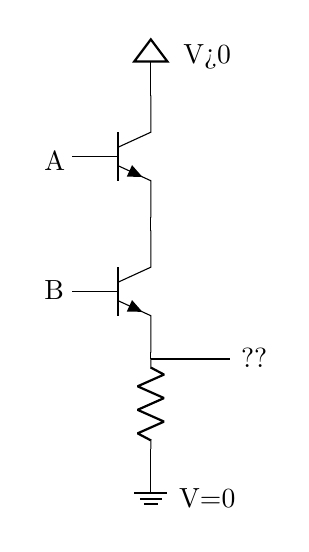
\begin{tikzpicture}
				% Paths, nodes and wires:
				\node[ground] at (1, 4.286){};
				\node[sground, yscale=-1] at (1, 9){};
				\node[shape=rectangle, minimum width=1.197cm, minimum height=0.679cm] at (1.812, 9.429){} node[anchor=north west, align=left, text width=0.809cm, inner sep=6pt] at (1.196, 9.786){V>0};
				\node[shape=rectangle, minimum width=0.608cm, minimum height=0.536cm] at (1.464, 3.857){} node[anchor=north west, align=left, text width=0.22cm, inner sep=6pt] at (1.143, 4.143){V=0};
				\node[npn] at (1, 8.143){};
				\node[npn] at (1, 6.429){};
				\draw (1, 5.571) to[american resistor, /tikz/circuitikz/bipoles/length=1.12cm] (1, 4.429);
				\draw (1, 9) -- (1, 8.913);
				\draw (1, 7.373) -- (1, 7.199);
				\draw (1, 5.659) -- (1, 5.571);
				\draw (1, 4.429) -- (1, 4.286);
				\draw (1, 5.571) -- (2, 5.571);
				\draw (0.16, 6.429) -- (0, 6.429);
				\draw (0.16, 8.143) -- (0, 8.143);
				\node[shape=rectangle, minimum width=0.679cm, minimum height=0.679cm] at (-0.214, 8.071){} node[anchor=north west, align=left, text width=0.291cm, inner sep=6pt] at (-0.571, 8.429){A};
				\node[shape=rectangle, minimum width=0.679cm, minimum height=0.679cm] at (-0.214, 6.429){} node[anchor=north west, align=left, text width=0.291cm, inner sep=6pt] at (-0.571, 6.786){B};
				\node[shape=rectangle, minimum width=0.679cm, minimum height=0.679cm] at (2.286, 5.571){} node[anchor=north west, align=left, text width=0.291cm, inner sep=6pt] at (1.929, 5.929){??};
			\end{tikzpicture}
		\end{column}
	\end{columns}
\end{frame}




\Subsection{Resistors}



\begin{frame}{What is a resistor?}
	light bulb

	ceramic

	the coils in your toaster

	something to soak up energy

	if you run electric current through it and it gets hot, it's a resistor (or at least has resistance)
\end{frame}


\begin{frame}{Voltage Drops in the Resistor}
	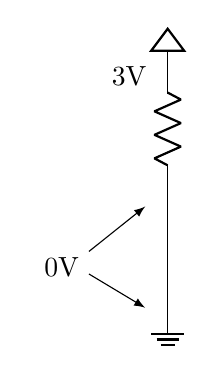
\begin{tikzpicture}
		% Paths, nodes and wires:
		\node[ground] at (2.571, 5.659){};
		\draw (2.571, 8.484) to[american resistor, /tikz/circuitikz/bipoles/length=1.12cm] (2.571, 7.199);
		\node[sground, yscale=-1] at (2.571, 8.484){};
		\node[shape=rectangle, minimum width=0.608cm, minimum height=0.536cm] at (1.964, 8.571){} node[anchor=north west, align=left, text width=0.22cm, inner sep=6pt] at (1.643, 8.857){3V};
		\node[shape=rectangle, minimum width=0.608cm, minimum height=0.536cm] at (1.107, 6.143){} node[anchor=north west, align=left, text width=0.22cm, inner sep=6pt] at (0.786, 6.429){0V};
		\draw[-latex] (1.571, 6.286) -- (2.286, 6.857);
		\draw[-latex] (1.571, 6) -- (2.286, 5.571);
		\draw (2.571, 7.199) -- (2.571, 5.659);
	\end{tikzpicture}
\end{frame}




\begin{frame}{Voltage only drops if it has somewhere to go}

Voltage drop only happens if electricity is flowing. Otherwise the voltage is the same everywhere

	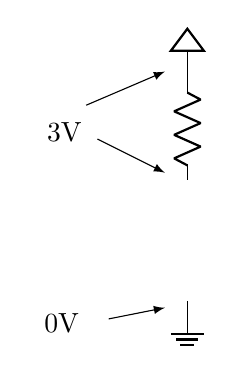
\begin{tikzpicture}
		% Paths, nodes and wires:
		\node[ground] at (2.571, 5.659){};
		\draw (2.571, 8.484) to[american resistor, /tikz/circuitikz/bipoles/length=1.12cm] (2.571, 7.199);
		\node[sground, yscale=-1] at (2.571, 8.484){};
		\node[shape=rectangle, minimum width=0.608cm, minimum height=0.536cm] at (0.893, 7.857){} node[anchor=north west, align=left, text width=0.22cm, inner sep=6pt] at (0.571, 8.143){3V};
		\node[shape=rectangle, minimum width=0.608cm, minimum height=0.536cm] at (0.857, 5.429){} node[anchor=north west, align=left, text width=0.22cm, inner sep=6pt] at (0.536, 5.714){0V};
		\draw[-latex] (1.286, 8.143) -- (2.286, 8.571);
		\draw[-latex] (1.429, 7.714) -- (2.286, 7.286);
		\draw[-latex] (1.571, 5.429) -- (2.286, 5.571);
	\end{tikzpicture}
\end{frame}


\begin{frame}{NOT ALLOWED}
	\begin{columns}
		\begin{column}{0.5\textwidth}
			We assume:
			\begin{itemize}
				\item Top rail fixed at V>0
				\item Bottom rail fixed at 0V
				\item Wires have zero resistance
			\end{itemize}
		\end{column}
		\begin{column}{0.5\textwidth}
			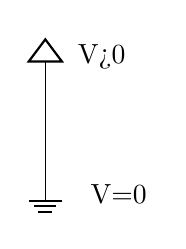
\begin{tikzpicture}
				% Paths, nodes and wires:
				\node[ground] at (1, 8){};
				\node[sground, yscale=-1] at (1, 9){};
				\node[shape=rectangle, minimum width=1.197cm, minimum height=0.679cm] at (1.813, 9.429){} node[anchor=north west, align=left, text width=0.809cm, inner sep=6pt] at (1.196, 9.786){V>0};
				\node[shape=rectangle, minimum width=0.608cm, minimum height=0.536cm] at (1.679, 7.714){} node[anchor=north west, align=left, text width=0.22cm, inner sep=6pt] at (1.357, 8){V=0};
				\draw (1, 9) -- (1, 8);
			\end{tikzpicture}		\end{column}
	\end{columns}

	If you try to build this, one of those assumptions will fail. What might that look like?

\end{frame}


\Subsection{Transistors}

\begin{frame}{Historical Transistors}
	\includegraphics[width=0.5\columnwidth]{images/tube-transistor-wiki}
\end{frame}


\begin{frame}{Modern Transistors}
	\includegraphics[width=\columnwidth]{images/semiconductor-transistor-overkill}
\end{frame}



\begin{frame}{Transistor Behavior}

	https://www.101computing.net/creating-logic-gates-using-transistors/

	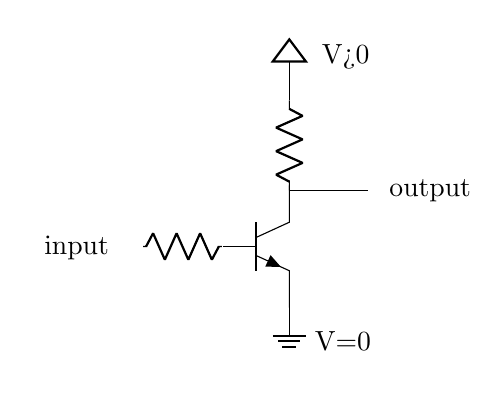
\begin{tikzpicture}
		% Paths, nodes and wires:
		\node[ground] at (1, 6.286){};
		\node[sground, yscale=-1] at (1, 9){};
		\node[shape=rectangle, minimum width=1.197cm, minimum height=0.679cm] at (1.813, 9.429){} node[anchor=north west, align=left, text width=0.809cm, inner sep=6pt] at (1.196, 9.786){V>0};
		\node[shape=rectangle, minimum width=0.608cm, minimum height=0.536cm] at (1.429, 5.857){} node[anchor=north west, align=left, text width=0.22cm, inner sep=6pt] at (1.107, 6.143){V=0};
		\draw (1, 8.857) to[american resistor, /tikz/circuitikz/bipoles/length=1.12cm] (1, 7.714);
		\draw (1, 9) -- (1, 8.857);
		\draw (1, 7.714) -- (2, 7.714);
		\node[shape=rectangle, minimum width=1.197cm, minimum height=0.679cm] at (2.67, 7.714){} node[anchor=north west, align=left, text width=0.809cm, inner sep=6pt] at (2.054, 8.071){output};
		\draw (-0.857, 7) to[american resistor, /tikz/circuitikz/bipoles/length=1.12cm] (0.143, 7);
		\draw (0.286, 7) -- (0.408, 7);
		\node[npn] at (1, 7){};
		\node[shape=rectangle, minimum width=1.197cm, minimum height=0.679cm] at (-1.714, 7){} node[anchor=north west, align=left, text width=0.809cm, inner sep=6pt] at (-2.33, 7.357){input};
	\end{tikzpicture}
\end{frame}


\begin{frame}{Transistor Behavior}
	\begin{columns}
		\begin{column}{0.5\textwidth}
			\usetikzlibrary{shapes.geometric}
			\begin{tikzpicture}
				% Paths, nodes and wires:
				\node[ground] at (1, 6.286){};
				\node[sground, yscale=-1] at (1, 9){};
				\node[shape=rectangle, minimum width=1.197cm, minimum height=0.679cm] at (1.813, 9.429){} node[anchor=north west, align=left, text width=0.809cm, inner sep=6pt] at (1.196, 9.786){V>0};
				\node[shape=rectangle, minimum width=0.608cm, minimum height=0.536cm] at (1.429, 5.857){} node[anchor=north west, align=left, text width=0.22cm, inner sep=6pt] at (1.107, 6.143){V=0};
				\draw (1, 8.857) to[american resistor, /tikz/circuitikz/bipoles/length=1.12cm] (1, 7.714);
				\node[shape=ellipse, draw, line width=1pt, dash pattern={on 1pt off 2pt}, minimum width=1.149cm, minimum height=1.108cm] at (1, 7){};
				\node[shape=rectangle, minimum width=1.197cm, minimum height=0.965cm] at (-1.33, 7.143){} node[anchor=north west, align=left, text width=0.809cm, inner sep=6pt] at (-1.946, 7.643){input\\V>0};
				\draw (1, 6.571) to[cute closed switch] (1, 7.429);
				\draw (1, 9) -- (1, 8.857);
				\draw (1, 7.714) -- (1, 7.429);
				\draw (1, 6.571) -- (1, 6.286);
				\draw (1, 7.714) -- (2, 7.714);
				\node[shape=rectangle, minimum width=1.197cm, minimum height=0.679cm] at (2.67, 7.714){} node[anchor=north west, align=left, text width=0.809cm, inner sep=6pt] at (2.054, 8.071){??};
				\draw (-0.714, 7) to[american resistor, /tikz/circuitikz/bipoles/length=1.12cm] (0.286, 7);
				\draw (0.286, 7) -- (0.408, 7);
			\end{tikzpicture}
		\end{column}
		\begin{column}{0.5\textwidth}
			\usetikzlibrary{shapes.geometric}
			\begin{tikzpicture}
				% Paths, nodes and wires:
				\node[ground] at (1, 6.286){};
				\node[sground, yscale=-1] at (1, 9){};
				\node[shape=rectangle, minimum width=1.197cm, minimum height=0.679cm] at (1.813, 9.429){} node[anchor=north west, align=left, text width=0.809cm, inner sep=6pt] at (1.196, 9.786){V>0};
				\node[shape=rectangle, minimum width=0.608cm, minimum height=0.536cm] at (1.429, 5.857){} node[anchor=north west, align=left, text width=0.22cm, inner sep=6pt] at (1.107, 6.143){V=0};
				\draw (1, 8.857) to[american resistor, /tikz/circuitikz/bipoles/length=1.12cm] (1, 7.714);
				\node[shape=ellipse, draw, line width=1pt, dash pattern={on 1pt off 2pt}, minimum width=1.149cm, minimum height=1.108cm] at (1, 7){};
				\node[shape=rectangle, minimum width=1.197cm, minimum height=0.965cm] at (-1.33, 7.143){} node[anchor=north west, align=left, text width=0.809cm, inner sep=6pt] at (-1.946, 7.643){input\\V=0};
				\draw (1, 6.571) to[cute open switch] (1, 7.429);
				\draw (1, 9) -- (1, 8.857);
				\draw (1, 7.714) -- (1, 7.429);
				\draw (1, 6.571) -- (1, 6.286);
				\draw (1, 7.714) -- (2, 7.714);
				\node[shape=rectangle, minimum width=1.197cm, minimum height=0.679cm] at (2.67, 7.714){} node[anchor=north west, align=left, text width=0.809cm, inner sep=6pt] at (2.054, 8.071){??};
				\draw (-0.714, 7) to[american resistor, /tikz/circuitikz/bipoles/length=1.12cm] (0.286, 7);
				\draw (0.286, 7) -- (0.408, 7);
			\end{tikzpicture}
		\end{column}
	\end{columns}
\end{frame}


\begin{frame}{Transistor Behavior}
	\begin{columns}
		\begin{column}{0.5\textwidth}
			\usetikzlibrary{shapes.geometric}
			\begin{tikzpicture}
				% Paths, nodes and wires:
				\node[ground] at (1, 6.286){};
				\node[sground, yscale=-1] at (1, 9){};
				\node[shape=rectangle, minimum width=1.197cm, minimum height=0.679cm] at (1.813, 9.429){} node[anchor=north west, align=left, text width=0.809cm, inner sep=6pt] at (1.196, 9.786){V>0};
				\node[shape=rectangle, minimum width=0.608cm, minimum height=0.536cm] at (1.429, 5.857){} node[anchor=north west, align=left, text width=0.22cm, inner sep=6pt] at (1.107, 6.143){V=0};
				\draw (1, 8.857) to[american resistor, /tikz/circuitikz/bipoles/length=1.12cm] (1, 7.714);
				\node[shape=ellipse, draw, line width=1pt, dash pattern={on 1pt off 2pt}, minimum width=1.149cm, minimum height=1.108cm] at (1, 7){};
				\node[shape=rectangle, minimum width=1.197cm, minimum height=0.965cm] at (-1.33, 7.143){} node[anchor=north west, align=left, text width=0.809cm, inner sep=6pt] at (-1.946, 7.643){input\\V>0};
				\draw (1, 6.571) to[cute closed switch] (1, 7.429);
				\draw (1, 9) -- (1, 8.857);
				\draw (1, 7.714) -- (1, 7.429);
				\draw (1, 6.571) -- (1, 6.286);
				\draw (1, 7.714) -- (2, 7.714);
				\node[shape=rectangle, minimum width=1.197cm, minimum height=0.679cm] at (2.67, 7.714){} node[anchor=north west, align=left, text width=0.809cm, inner sep=6pt] at (2.054, 8.071){output\\V=0};
				\draw (-0.714, 7) to[american resistor, /tikz/circuitikz/bipoles/length=1.12cm] (0.286, 7);
				\draw (0.286, 7) -- (0.408, 7);
			\end{tikzpicture}
		\end{column}
		\begin{column}{0.5\textwidth}
			\usetikzlibrary{shapes.geometric}
			\begin{tikzpicture}
				% Paths, nodes and wires:
				\node[ground] at (1, 6.286){};
				\node[sground, yscale=-1] at (1, 9){};
				\node[shape=rectangle, minimum width=1.197cm, minimum height=0.679cm] at (1.813, 9.429){} node[anchor=north west, align=left, text width=0.809cm, inner sep=6pt] at (1.196, 9.786){V>0};
				\node[shape=rectangle, minimum width=0.608cm, minimum height=0.536cm] at (1.429, 5.857){} node[anchor=north west, align=left, text width=0.22cm, inner sep=6pt] at (1.107, 6.143){V=0};
				\draw (1, 8.857) to[american resistor, /tikz/circuitikz/bipoles/length=1.12cm] (1, 7.714);
				\node[shape=ellipse, draw, line width=1pt, dash pattern={on 1pt off 2pt}, minimum width=1.149cm, minimum height=1.108cm] at (1, 7){};
				\node[shape=rectangle, minimum width=1.197cm, minimum height=0.965cm] at (-1.33, 7.143){} node[anchor=north west, align=left, text width=0.809cm, inner sep=6pt] at (-1.946, 7.643){input\\V=0};
				\draw (1, 6.571) to[cute open switch] (1, 7.429);
				\draw (1, 9) -- (1, 8.857);
				\draw (1, 7.714) -- (1, 7.429);
				\draw (1, 6.571) -- (1, 6.286);
				\draw (1, 7.714) -- (2, 7.714);
				\node[shape=rectangle, minimum width=1.197cm, minimum height=0.679cm] at (2.67, 7.714){} node[anchor=north west, align=left, text width=0.809cm, inner sep=6pt] at (2.054, 8.071){output\\V>0};
				\draw (-0.714, 7) to[american resistor, /tikz/circuitikz/bipoles/length=1.12cm] (0.286, 7);
				\draw (0.286, 7) -- (0.408, 7);
			\end{tikzpicture}
		\end{column}
	\end{columns}
\end{frame}



\begin{frame}{Why two resistors?}

In many cases, we can get away with just one resistor. The previous example had two. Why?

Always need a resistor between a voltage source and ground. Transistors have internal resistance but it's very small. Easy to burn them out

\end{frame}





\begin{frame}{More Complex Example}
	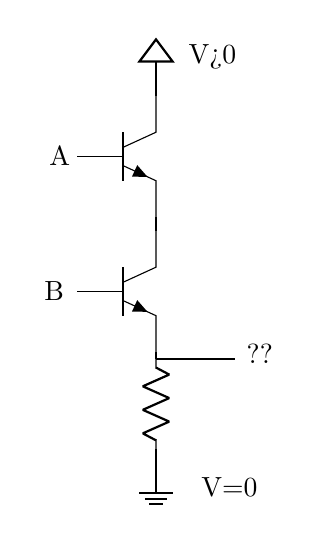
\begin{tikzpicture}
		% Paths, nodes and wires:
		\node[ground] at (1, 4.286){};
		\node[sground, yscale=-1] at (1, 9){};
		\node[shape=rectangle, minimum width=1.197cm, minimum height=0.679cm] at (1.813, 9.429){} node[anchor=north west, align=left, text width=0.809cm, inner sep=6pt] at (1.196, 9.786){V>0};
		\node[shape=rectangle, minimum width=0.608cm, minimum height=0.536cm] at (1.679, 4){} node[anchor=north west, align=left, text width=0.22cm, inner sep=6pt] at (1.357, 4.286){V=0};
		\draw (1, 5.571) to[american resistor, /tikz/circuitikz/bipoles/length=1.12cm] (1, 4.429);
		\node[npn] at (1, 8.143){};
		\node[npn] at (1, 6.429){};
		\draw (1, 9) -- (1, 8.913);
		\draw (1, 7.373) -- (1, 7.199);
		\draw (1, 5.659) -- (1, 5.571);
		\draw (1, 5.571) -- (2, 5.571);
		\draw (0.16, 8.143) -- (0, 8.143);
		\draw (0.16, 6.429) -- (0, 6.429);
		\draw (1, 4.429) -- (1, 4.286);
		\node[shape=rectangle, minimum width=0.668cm, minimum height=0.65cm] at (-0.22, 8.143){} node[anchor=north west, align=left, text width=0.28cm, inner sep=6pt] at (-0.571, 8.485){A};
		\node[shape=rectangle, minimum width=0.668cm, minimum height=0.65cm] at (-0.286, 6.429){} node[anchor=north west, align=left, text width=0.28cm, inner sep=6pt] at (-0.637, 6.771){B};
		\node[shape=rectangle, minimum width=0.668cm, minimum height=0.65cm] at (2.286, 5.628){} node[anchor=north west, align=left, text width=0.28cm, inner sep=6pt] at (1.934, 5.971){??};
	\end{tikzpicture}
\end{frame}




% what is a transistor
% building logic gates

% TEST 3 TOPICS

\Section{Instruction Pipelining}

\Subsection{FDEW Cycle}

\Subsection{Pipelining}

\Subsection{Hazards}

% pipelining
% data hazards
% control hazards

\Section{Assembly Conditionals and Loops}

% b, beq, bne, ...
% if/else
% while loops
% for loops

\input{sections/multiprocessing.tex}
% booting
% forking
% threads, cores, processes
% async


\Section{Appendix}


\Subsection{Raspberry Pi Setup}


\begin{frame}{Pi Setup: Kit Contents}
	\begin{columns}
		\begin{column}{0.5\textwidth}
			\begin{enumerate}
				\item Pi case
				\item Raspberry Pi (in box)
				\item Heat sinks
				\item Power cord
				\item Ethernet to USB adapter
				\item Ethernet cord
				\item USB 2 to USB 3 adapter
				\item SD Card
				\item Accessory case
			\end{enumerate}
		\end{column}
		\begin{column}{0.5\textwidth}
			\includegraphics[width=\columnwidth]{images/pi-kit-contents}
		\end{column}
	\end{columns}
\end{frame}


\begin{frame}{Pi Setup: Apply Heat Sinks}
	\begin{columns}
		\begin{column}{0.5\textwidth}
			\includegraphics[width=\columnwidth]{images/pi-heat-sinks-1}
		\end{column}
		\begin{column}{0.5\textwidth}
			\includegraphics[width=\columnwidth]{images/pi-heat-sinks-2}
		\end{column}
	\end{columns}
\end{frame}

\begin{frame}{Pi Setup: Apply Nonslip Nubs}
	\includegraphics[width=\columnwidth]{images/pi-case-nubs}
\end{frame}

\begin{frame}{Pi Setup: Install in Case}
	\includegraphics[width=\columnwidth]{images/pi-in-case}
\end{frame}

\begin{frame}{Pi Setup: SD Card}
	\begin{columns}
		\begin{column}{0.5\textwidth}
			\includegraphics[width=\columnwidth]{images/pi-sd-card-1}
		\end{column}
		\begin{column}{0.5\textwidth}
			\includegraphics[width=\columnwidth]{images/pi-sd-card-2}
		\end{column}
	\end{columns}
\end{frame}

\begin{frame}{Pi Setup: Connect to Laptop}
	\includegraphics[width=\columnwidth]{images/pi-to-laptop}
\end{frame}

\begin{frame}{Pi Setup: Connect to Power}
\end{frame}

\begin{frame}{Laptop Setup: Enable WiFi}
	\includegraphics[width=\columnwidth]{images/pi-network-settings}
\end{frame}

\begin{frame}{Laptop Setup: Install VSCode}
	\includegraphics[width=\columnwidth]{images/vscode-remote-ssh}
\end{frame}

\begin{frame}{Laptop Setup: Add Remote Connection}
	\includegraphics[width=\columnwidth]{images/vscode-add-remote}
\end{frame}

\begin{frame}{Laptop Setup: SSH Login}
	\begin{itemize}
		\item Default username/password is raspberri/pi
		\item Make sure to update username and password
	\end{itemize}
\end{frame}


\Subsection{CSGit Setup}

% vscode setup
% pi setup
% csgit setup


\end{document}
% why study assembly?
% global variables
% mov
% printf
% ldr
% scanf
% add, mul


\documentclass{beamer}
\usepackage[utf8]{inputenc}
\usepackage[T1]{fontenc}
\usepackage{circuitikz}

\usepackage{multirow}

\title{CS241: Hardware Design}
\date{\today}
\author[Fyfe and Lynn]{Charles Fyfe and Melissa Lynn}
\institute{St Olaf College}

\usetheme{grape}

\usepackage{parskip}
\usepackage{multicol}
\usepackage{graphicx}
% make \oplus look nice
\usepackage{amssymb}

\begin{document}


\titlepage

% just sections up top
\setcounter{tocdepth}{1}

\begin{frame}{Outline}

	\begin{multicols*}{2}
		\tableofcontents
	\end{multicols*}
\end{frame}

% show subsections later
\setcounter{tocdepth}{2}


\Section{Syllabus}

\begin{frame}{Course Overview}

	\includegraphics[width=\columnwidth]{images/dune-robot-hbo}

	{\center
		Thou shalt not make a machine in the likeless of a human mind
	}

	{\small \hfill
		The Orange Catholic Bible, Dune, Frank Herbert
	}
\end{frame}


\begin{frame}{Course Overview}

	Computers feel like magic. You type words. The machine does complex things. Especially in the era of large language models

	But it's not magic. Computers are made of semiconductors, metal, and magnets. Three different kinds of rocks

	This course is about demystifying the machine and exploring how, fundamentally, computers do what they do. Specifically, we'll be looking at:
	\begin{itemize}
		\item The fundamental components of a computer
		\item How data is stored on a computer
		\item Building electrical circuits to perform logic
		\item Programming in Assembly (a very low-level language)
	\end{itemize}
\end{frame}

\Subsection{Grading}

\begin{frame}{Course Grade Breakdown}
	\begin{itemize}
		\item Quizzes and final: 45\%
		\item Homework and labs: 45\%
		\item Participation: 10\%
	\end{itemize}
\end{frame}

\begin{frame}{Standards-Based Grading}
	\begin{itemize}
		\item There are nine standards in the class. Each is worth 5\% of your grade.
		\item There are three quizzes. Each quiz covers three standards.
		\item The final covers all nine standards.
		\item If you demonstrate proficiency on the quiz, you're done with that standard. Full credit. You can skip that part of the final.
		\item If you demonstrate partial proficiency on the quiz, you get half credit. Try again on the final for full credit.
		\item If you do not demonstrate proficiency on the quiz, you get no credit. You can still get full credit on the final!
	\end{itemize}
\end{frame}


\begin{frame}{Homework and Labs}
	\begin{itemize}
		\item One or more lab exercises for each standard. We start these together in class. You may need to finish on your own time.
		\item We will have a homework assignment for each standard.
		\item Please work together in small groups.
		\item Please ensure that the work you turn in reflects your own understanding.
	\end{itemize}
\end{frame}

\begin{frame}{Late Work Policy}
	Please try to get your work in on time.
	\begin{itemize}
		\item If you don't get your work done on time, you may fall behind in the class.
		\item Late work is inconvenient for the TAs. They will be grumpy and vindictive when they grade your work.
		\item TAs will have their own finals to worry about! Late work at the end of the semester might be refused.
	\end{itemize}
	If you need an extension, please reach out beforehand.
\end{frame}

\begin{frame}{Peer Reviews}
	\begin{itemize}
		\item Participation score (10\% of your total grade) is mostly based on peer reviews.
		\item Reviews will be short. Less than one page.
		\item You can get full credit here without too much trouble. Show up. Work together. Make it easy for your peers to say nice things about you.
		\item I recommend keeping notes over the course of the semester when someone is particularly helpful, insightful, etc. Good reviews have concrete examples.
	\end{itemize}
\end{frame}

\Subsection{Office Hours}

\begin{frame}{Office Hours}
	TODO
\end{frame}


\Subsection{Disability Accommodations}

\begin{frame}{Disability Accommodations}
	I am committed to supporting the learning of all students in my class. If you have already
	registered with Disability and Access (DAC) and have your letter of accommodations, please
	meet with me as soon as possible to discuss, plan, and implement your accommodations in the
	course. If you have or think you have a disability (learning, sensory, physical, chronic health,
	mental health or attentional), please contact Disability and Access staff at 507-786-3288 or by visiting \href{https://wp.stolaf.edu/academic-support/dac}{their website}.


	If you have an accommodation that allows you extra time or a low distraction environment for
	quizzes and exams, please email me at least three days before each quiz or exam, so that I can
	make sure to reserve a room.
\end{frame}


\Subsection{Religious Accommodations}

\begin{frame}{Religious Accommodations}
	As part of my commitment to make St Olaf an inclusive community, I will provide students with
	reasonable religious accommodations. If you will be missing class for a religious observance or
	require another religious accommodation, please meet with me to discuss these.
\end{frame}


\Subsection{Academic Integrity}

\begin{frame}{Academic Integrity}

	Plagiarism is a serious academic offense. Hand in your own work. Give credit appropriately when you draw from the work of others. For more information please see:

	\begin{itemize}
		\item \href{https://wp.stolaf.edu/facultyhandbook/academic-integrity-faculty-handbook-category-2}{Faculty Handbook: Academic Integrity}
		\item \href{https://wp.stolaf.edu/honorcouncil/}{The Honor Code}
		\item \href{https://wp.stolaf.edu/roadmap-to-academic-integrity}{Roadmap to Academic Integrity}
	\end{itemize}

	Work that violates this policy will typically receive no credit. In especially serious cases the penalty can be an F in the course.
\end{frame}

\Subsection{AI Use Policy}

\begin{frame}{AI Usage Policy}
	Please not submit AI work as your own.

	You may use AI tools when studying, but be careful. These tools are very good with mainstream languages like Python. We're working with Assembly, which is very much \textbf{not} a mainstream language.

\end{frame}


\Subsection{St Olaf Land Acknowledgement}

\begin{frame}{St Olaf Land Acknowledgement}
	We stand on the homelands of the Wahpekute Band of the Dakota Nation. We honor with
	gratitude the people who have stewarded the land throughout the generations and their ongoing
	contributions to this region. We acknowledge the ongoing injustices that we have committed
	against the Dakota Nation, and we wish to interrupt this legacy, beginning with acts of healing
	and honest storytelling about this place.

	For more information about land acknowledgement statements at St Olaf, please see \href{https://wp.stolaf.edu/education/land-acknowledgement/}{here} and \href{https://wp.stolaf.edu/equity-inclusion/land-acknowledgement/}{here}.
\end{frame}


\Subsection{Statement of Inclusivity}

\begin{frame}{Statement of Inclusivity}
	In keeping with St. Olaf College's mission statement, this class strives to be an inclusive
	learning community, respecting those of differing backgrounds and beliefs. As a community, we
	aim to be respectful to all citizens in this class, regardless of race, ethnicity, religion, gender or
	sexual orientation.
\end{frame}


\Subsection{Gender Pronouns}

\begin{frame}{Gender Pronouns}
	This course affirms people of all gender expressions and gender identities. If you go by a
	different name than what is on the class roster, please let me know.

	Using correct gender
	pronouns is important to me, so you are encouraged to share your pronouns with me and
	correct me if a mistake is made. If you have any questions or concerns, please do not hesitate
	to contact me.
\end{frame}


\Subsection{Multilingual Student Support}

\begin{frame}{Multilingual Student Support}
	I am committed to making course content accessible to all students. If English is not your first
	language and this causes you concern about the course, please speak with me. Students who
	would like extra support with writing or speaking in English can also contact the language support specialist (\href{mailto:berryag@stolaf.edu}{berryag@stolaf.edu}) in the Academic Success Center.
\end{frame}


\Subsection{Mental Health}

\begin{frame}{Mental Health}

	I greatly value your experience in this class, and it is my duty to facilitate a safe, caring, and
	productive learning environment.

	I recognize that you may experience a range of emotional, physical, and/or psychological
	issues, both in and out of the classroom, that may distract you from your learning.

	If you are experiencing such issues, please do not hesitate to come see me. I am here to listen.
	We can also discuss what further resources might be available to you.
\end{frame}

\Subsection{Required Referrals}


\begin{frame}{Required Referrals}
	You are welcome to talk to me about circumstances outside the course that
	affect your classroom experience or acadmic performance. However, please keep
	in mind that I am required to refer cases of discrimination, harassment,
	sexual misconduct, and violence.

	Here are some resources where you can share privately:

	\begin{itemize}
		\item Boe House Counseling Center
		\item College Pastors and Chaplains
		\item Sexual Assault Resource Network (SARN)
		\item Health Services
		\item TimelyCare
	\end{itemize}
\end{frame}




\Subsection{St. Olaf Pride Statement}

\begin{frame}{St. Olaf Pride Statement}
	As an Ole, I will practice:
	\begin{itemize}
		\item Passion for learning and pursuit of vocation
		\item Respect for the worth and dignity of all people
		\item Integrity at all times, in all circumstances
		\item Dedication to a life of service, and
		\item Engagement with my community and the world.
	\end{itemize}
\end{frame}









\Subsection{Important Links}

\begin{frame}{Important Links}
	\begin{itemize}
		\item ARM tutorial https://computerscience.chemeketa.edu/armTutorial/index.html
		\item ARM simulator https://cpulator.01xz.net/?sys=arm
		\item circuit simulator: https://circuitverse.org/simulator
	\end{itemize}
\end{frame}





% TEST 1 TOPICS


\Section{Data Representation}

\begin{frame}{How do computers store information?}
	Computers work using electrical signals which can be on or off. If we let:
	\begin{itemize}
		\item On means 1
		\item Off means 0
	\end{itemize}
	We can use sequences of 0s and 1s to represent information
\end{frame}

\Subsection{Positive Integers in Binary}

\begin{frame}{Numbers in Base Ten (aka Decimal)}
	Let's start by talking about how we write numbers normally.

	For example, let's look at the number 109:
	\begin{align*}
		109 & = 100 \;+\; 0 \;+\; 9                                   \\
		    & = 1 \Times 10^2 \;+\; 0 \Times 10^1 \;+\; 9 \Times 10^0
	\end{align*}
	This way of writing numbers is called base ten.
	We use ten digits (0 to 9 inclusive) and each position in the number is scaled by a power of ten.

	In terms of math, there is nothing special about base ten. We probably use it
	because we have ten fingers. Some ancient civilizations used sompletely
	different systems for counting!
\end{frame}

\begin{frame}{Numbers in Base Two (aka Binary)}
	Computers don't have fingers. They express everything as sequences of 1s and 0s. This format is called binary:

	\begin{align*}
		0b1101101 & =
		1 \Times 2^6 +
		1 \Times 2^5 +
		0 \Times 2^4 +
		1 \Times 2^3 +
		1 \Times 2^2 +
		0 \Times 2^1 +
		1 \Times 2^0                              \\
		          & = 64 + 32 + 0 + 8 + 4 + 0 + 1 \\
		          & = 109                         \\
	\end{align*}
	Importantly: we always use the prefix ``0b'' to avoid confusion when writing numbers in binary.

	1101 is one thousand one hundred and one

	0b1101 is thirteen
\end{frame}

\begin{frame}{Converting from Decimal to Binary}

	If the number is odd, append a 1 on the left. Otherwise, append a 0. Then
	divide your decimal number by two and ignore any remainder. Repeat until your
	decimal number is zero. \\

	For example, starting with 58:

	\begin{itemize}
		\item 58 is even, so append \Highlight{0}. Divide by two, leaving 29.
		\item 29 is odd, so append \Highlight{1}0. Divide by two, leaving 14.
		\item 14 is even, so append \Highlight{0}10. Divide by two, leaving 7.
		\item 7 is odd, so append \Highlight{1}010. Divide by two, leaving 3.
		\item 3 is odd, so append \Highlight{1}1010. Divide by two, leaving 1.
		\item 1 is odd, so append \Highlight{1}11010. Divide by two, leaving 0.
	\end{itemize}

	So 58 in binary is 0b111010.

\end{frame}

\begin{frame}{Converting from Binary to Decimal}

	We can confirm by converting back. The rightmost bit is worth 1, then 2, then
	4, and so on:

	\begin{align*}
		0b111010 & =
		1 \Times 2^5 +
		1 \Times 2^4 +
		1 \Times 2^3 +
		0 \Times 2^2 +
		1 \Times 2^1 +
		0 \Times 2^0                          \\
		         & = 32 + 16  + 8 + 0 + 2 + 0 \\
		         & = 58
	\end{align*}

\end{frame}

\begin{frame}{Addition in Binary}
	Binary addition works just like decimal addition.
	Start from the right, add straight down, and carry when you run out of digits.

	For example:
	\[
		\begin{array}{ccccccccc}
			1 & 1 & 1 & 1 & 1 &   &   &   &   \\
			  & 0 & 0 & 1 & 1 & 1 & 0 & 0 & 0 \\
			+ & 1 & 1 & 1 & 0 & 1 & 0 & 0 & 1 \\
			\hline
			1 & 0 & 0 & 1 & 0 & 0 & 0 & 0 & 1 \\
		\end{array}
	\]

	What happens if we try to perform this operation but we only have 8 bits to
	store the answer?
\end{frame}

\begin{frame}{Multiplication in Binary}
	Binary multiplication works just like decimal multiplication.
	Multiply the top number by the rightmost digit of the bottom number.
	Then move to the next line, add a zero, and repeat for the next digit.
	Finally, add up the lines. For example:
	\[
		\begin{array}{cccccc}
			  &   &        & 1 & 1 & 0 \\
			  &   & \times & 1 & 0 & 1 \\
			\hline
			  &   &        & 1 & 1 & 0 \\
			  &   & 0      & 0 & 0 & 0 \\
			+ & 1 & 1      & 0 & 0 & 0 \\
			\hline
			  & 1 & 1      & 1 & 1 & 0 \\
		\end{array}
	\]
\end{frame}

\begin{frame}{Division in Binary}
	To divide by 2, shift the bits one place to the right. \\

	To divide by 4, shift the bits two places to the right. \\

	That's about as deep as we go in this class. If you're curious to learn more,
	see the textbook.

\end{frame}



\Subsection{Hexadecimal}

\begin{frame}{What? Why?}

	Binary is how machines store data. But writing out binary by hand is a chore.
	In practice, it's often convenient to use hexadecimal (base 16) instead.

	\begin{itemize}
		\item Decimal uses ten digits, 0-9
		\item Binary uses two digits, 0 and 1
		\item Hexadecimal uses sixteen digits: 0-9 along with A-F
	\end{itemize}
	Hexadecimal values are always prefixed with ``0x'' to avoid ambiguity.
\end{frame}

\begin{frame}{Converting Between Binary and Hexadecimal}

	Converting back and forth between binary and hexadecimal does not require any
	math! Every four bits become one hex digit.
	\begin{align*}
		0b0000 & = 0x0 = 0 & 0b1000 & = 0x8 = 8  \\
		0b0001 & = 0x1 = 1 & 0b1001 & = 0x9 = 9  \\
		0b0010 & = 0x2 = 2 & 0b1010 & = 0xA = 10 \\
		0b0011 & = 0x3 = 3 & 0b1011 & = 0xB = 11 \\
		0b0100 & = 0x4 = 4 & 0b1100 & = 0xC = 12 \\
		0b0101 & = 0x5 = 5 & 0b1101 & = 0xD = 13 \\
		0b0110 & = 0x6 = 6 & 0b1110 & = 0xE = 14 \\
		0b0111 & = 0x7 = 7 & 0b1111 & = 0xF = 15 \\
	\end{align*}
\end{frame}

\begin{frame}{Converting Hexadecimal to Decimal}

	Hexadecimal is base 16. So each place corresponds to a power of 16.

	\begin{align*}
		0x3AB & = 3 \times 16^2 + 10 \times 16^1 + 11 \times 16^0 \\
		      & = 3 \times 256 + 10 \times 16 + 11 \times 1       \\
		      & = 768 + 160 + 11                                  \\
		      & = 954                                             \\
	\end{align*}

	Hexadecimal is very compact! These numbers get big fast

\end{frame}

\begin{frame}{Arithmetic in Hexadecimal}

	Addition and multiplication work in hexadecimal just like they do in binary and
	decimal. Just be careful about carrying.

	\[
		\begin{array}{ccccc}
			1 &   &   & 1 &   \\
			  & 4 & 1 & 7 & B \\
			+ & C & 2 & 0 & F \\
			\hline
			1 & 0 & 3 & 8 & A \\
		\end{array}
	\]

\end{frame}






\Subsection{Negatives in Binary}

\begin{frame}{First Attempt: Signed Magnitude}

	We can use the first digit to hold the sign, then the rest of the digits to
	hold magnitue:

	\begin{itemize}
		\item 0b\Highlight{0}1011001 is positive 10110001, so 89
		\item 0b\Highlight{1}1011001 is negative 1011001, so -89
	\end{itemize}

	This is nice and straightforward!

\end{frame}

\begin{frame}{Addition and Subtraction with Signed Magnitude}
	Adding positive numbers works just the same. But what happens if we throw a minus sign in there?

	For example, let's look at 12 - 5. First, rewrite it as 12 + (-5). Then:

	\[
		\begin{array}{ccccccccc}
			  & 0 & 0 & 0 & 0 & 1 & 1 & 0 & 0 \\
			+ & 1 & 0 & 0 & 0 & 0 & 1 & 0 & 1 \\
			\hline
			  & ? & ? & ? & ? & ? & ? & ? & ? \\
		\end{array}
	\]

	We know the result should be 7 (0b00000111). But our regular rules for addition
	do not get us there.
\end{frame}

\begin{frame}{Zero with Signed Magnitude}

	Using signed magnitude, 0b00000000 is zero.

	And 0b10000000 is negative zero (which is also zero).

	Using this convention, we have to worry about the difference between numerical
	equality and bitwise equality. That seems pretty messy.
\end{frame}

\begin{frame}{Can We Do Better?}
	Signed magnitude was a swing and a miss. What do we want when we talk about negative numbers?
	\begin{itemize}
		\item We want positive numbers to work like we expect
		\item We want 0b00000000 to be zero, with no ambiguity
		\item We want addition and subtraction to work the same for positive and negative
	\end{itemize}
\end{frame}

\begin{frame}{Another Idea: Two's Complement}
	We know 1 - 1 = 0. Put another way, 1 + (-1) = 0. Can we work backwards from there to figure out how to write -1?
	\[
		\begin{array}{ccccccccc}
			  & 0 & 0 & 0 & 0 & 0 & 0 & 0 & 1 \\
			+ & 1 & 1 & 1 & 1 & 1 & 1 & 1 & 1 \\
			\hline
			  & 0 & 0 & 0 & 0 & 0 & 0 & 0 & 0 \\
		\end{array}
	\]

	Remember: on a computer, our numbers have to fit in a set number of bits.
	Anything past that gets thrown away. This is called overflow. In this case,
	overflow works in our favor!
\end{frame}

\begin{frame}{Working Backwards from Zero}
	We can use the same trick to identify the rest of the negative numbers:
	\begin{itemize}
		\item 0b00000000 is 0
		\item 0b11111111 is -1
		\item 0b11111110 is -2
		\item 0b11111101 is -3
		\item 0b11111100 is -4
		\item etc
	\end{itemize}

\end{frame}

\begin{frame}{The Sign Bit (Again)}
	We only have 256 possible integers. How do we decide where the positives end and the negatives begin?

	Unsigned int: bits are worth 1, 2, 4, 8, 16, 32, 64, 128

	Signed magnitude: bits are worth $\pm1, \pm2, \pm4, \pm8, \pm16, \pm32, \pm64$,
	and the last bit tells us whether to use positive or negative (yikes)

	Two's complement: bits are worth 1, 2, 4, 8, 16, 32, 64, \Highlight{-128}

	Range of possible values is -128 to 127.
\end{frame}

\begin{frame}{Flipping Signs in Two's Complement}
	To flip the sign of a two's complement integer, flip all the bits then add 1. Ignore the overflow (if any). This works for both positive and negative numbers.

	For example:
	\begin{itemize}
		\item 55 is 0b01010111
		\item Flip the bits: 0b10101000, then add 1: 0b10101001
		\item So -55 is 0b10101001
		\item Flip the bits again: 0b01010110, add 1: 0b01010111
		\item So -(-55) = 55 = 0b01010111
	\end{itemize}

	What happens if we negate zero?
\end{frame}

\begin{frame}{Overflow}
	Overflow is important for two's complement. It ensures that positive zero and negative zero are the same. But it is also a constraint!

	Try adding 0b01101001 + 0b01011010:
	\[
		\begin{array}{ccccccccc}
			  &   & 1 & 1 & 1 &   &   &   &   \\
			  & 0 & 1 & 1 & 0 & 1 & 0 & 0 & 1 \\
			+ & 0 & 1 & 0 & 1 & 1 & 0 & 1 & 0 \\
			\hline
			  & 1 & 1 & 0 & 0 & 0 & 0 & 1 & 1 \\
		\end{array}
	\]

	These are two's complement numbers. Convert them to decimal. What just
	happened?

\end{frame}


\Subsection{Fractions and Decimals}

\begin{frame}{The Decimal Point}

	Sometimes we need to store numbers that aren't integers. \\

	Before we worry about binary, what does 21.867 mean? \\

	\begin{align*}
		21.867 & = 2 \Times 10^1 + 1 \Times 10^0 + 8 \Times ?? + 6 \Times ?? + 7 \Times ??
	\end{align*}

\end{frame}

\begin{frame}{The Decimal Point}

	In decimal:
	\begin{align*}
		21.867 & = 2 \Times 10^1 + 1 \Times 10^0 + 8 \Times 10^{-1} + 6 \Times 10^{-2} + 7 \Times 10^{-3}             \\
		       & =2 \Times 10 + 1 \Times 1 + 8 \Times \frac{1}{10} + 6 \Times \frac{1}{100} + 7 \Times \frac{1}{1000} \\
	\end{align*}

	In binary, we can use the same idea:
	\begin{align*}
		0b101.010 & = 1 \Times 2^2 + 0 \Times 2^1 + 1 \Times 2^0 + 0 \Times 2^{-1} + 1 \Times 2^{-2} + 0 \Times 2^{-3} \\
		          & = 1 \Times 4 + 0 + 1 \Times 1 + 0 + 1 \Times \frac{1}{4} + 0                                       \\
		          & = 5.25                                                                                             \\
	\end{align*}

\end{frame}

\begin{frame}{Fixed Point Representation}

	The computer just stores 1s and 0s, not decimal points. How do we distinguish
	these values?
	\begin{itemize}
		\item 0b0101110.1 = 46.5
		\item 0b010111.01 = 23.25
		\item 0b01011.101 = 11.625
	\end{itemize}

	One option is to specify the location of the decimal point ahead of time. For
	example, we could say that our eight-bit binary decimal always has two decimal
	bits. \\

	What is an upside of this approach? What is a downside?

\end{frame}

\begin{frame}{Floating Point Representation}

	Floating point numbers are a bit more complicated, but much more flexible. For
	a 16-bit floating point number we get:

	\begin{itemize}
		\item 1 bit for the sign
		\item 5 bits for the exponent (value -14 to 15)
		\item 10 bits for the significand (value 0 to 1023)
	\end{itemize}

	To turn those components into a value we use:
	\begin{align*}
		\text{value} & = (-1)^{\text{sign}} \times 2^{\text{exponent} - 15} \times \left(1 + \frac{\text{significand}}{1024} \right)
	\end{align*}

	Why offset the exponent?

	Why add 1 to the significand fraction?

\end{frame}

% Explanation here for the 127 offset: https://www.quora.com/Why-do-we-add-127-to-the-exponent-in-IEEE-754-floating-number-format-to-get-the-actual-exponent-value

\begin{frame}{Floating Point Examples}

	\begin{align*}
		\underbrace{0}_\text{sign} \; \underbrace{01111}_\text{exponent} \; \underbrace{0000000000}_\text{significand} & = (-1)^0 \times 2^{15 - 15} \times \left( 1 + \frac{0}{1024} \right) \\
		                                                                                                               & = 1 \times 2^0   \times \left( 1 + 0 \right)                         \\
		                                                                                                               & = 1                                                                  \\
	\end{align*}
	\begin{align*}
		0 \; 01101 \; 0101010101 & = (-1)^0 \times 2^{13 - 15} \times \left( 1 + \frac{341}{1024} \right) \\
		                         & \approx 0.33325195                                                     \\
	\end{align*}
	\begin{align*}
		1 \; 11110 \; 1111111111 & = (-1)^1 \times 2^{30 - 15} \times \left( 1 + \frac{1023}{1024} \right) \\
		                         & = -65504                                                                \\
	\end{align*}

	Why
\end{frame}

\begin{frame}{Floating Point Special Cases}

	\[
		\begin{array}{ccccr}
			0 & 00000 & 0000000000     & = 0          \\
			1 & 00000 & 0000000000     & = -0         \\
			0 & 11111 & 0000000000     & = \infty     \\
			1 & 11111 & 0000000000     & = -\infty    \\
			0 & 11111 & \text{nonzero} & = \text{NaN} \\
		\end{array}
	\]

	There's more to it than this. If you're curious, read up on subnormal numbers
	\href{https://en.wikipedia.org/wiki/Half-precision_floating-point_format}{here}

\end{frame}

\begin{frame}{Floating Point for Big Integers}

	If we're dealing with big numbers, floating point often works better than fixed
	point. This is true even if both formats use the same number of bits.

	\begin{itemize}
		\item 8-bit unsigned integer: max value 255
		\item 16-bit unsigned integer: max value 65,535
		\item 32-bit unsigned integer: max value 4.2 billion % 4,294,967,295
		\item 16-bit floating point: max value 65,504 (also handles negatives, fractions)
		\item 32-bit floating point: max value 340 billion billion billion billion (also handles negatives, fractions)
		      % 340,282,346,638,528,859,811,704,183,484,516,925,440 
	\end{itemize}

\end{frame}

\begin{frame}{Floating Point Limitations}

	So what's the catch?

\end{frame}

%        \item Convert 0b100110.10 from fixed-point binary to decimal.
%        \item Convert 23.75 from decimal to fixed-point binary.
%        \item Add fixed-point binary numbers 0b101101.01 + 0b010011.11. Convert to decimal to confirm your result.
%        \item Show that the 16-bit floating point expression ${1 \; 01000 \; 1100000000}$ is equal to -3.5 in decimal.

\Subsection{Beyond Numbers}

\begin{frame}{What else do computers store?}
	There are many cases where we want a computer to store non-numerical data:
	\begin{itemize}
		\item Text
		\item Colors
		\item Sounds
		\item Images
		\item Videos
		\item Websites
		\item Multiple things at once
	\end{itemize}
\end{frame}

\begin{frame}{Characters and Strings}
	\begin{itemize}
		\item Each character is represented by a number
		\item The most straightforward encoding is ASCII
		\item Modern use cases typically use Unicode (much bigger)
		\item To make a string, put a bunch of characters in a row
		\item Question: how do we identify the end of a string?
	\end{itemize}
\end{frame}

\begin{frame}{ASCII Table}
	\includegraphics[width=\columnwidth]{images/ascii-table}
\end{frame}

\begin{frame}{Colors and Images}
	\begin{itemize}
		\item A color can be described by three numbers (R, G, B)
		\item We can represent an image as a grid of colored pixels
		\item Question: do we need a null byte at the end of a pixel/row/image? Why or why not?
	\end{itemize}
	\includegraphics[width=\columnwidth]{images/mario-pixels}
\end{frame}

\begin{frame}{Sound}
	\begin{itemize}
		\item Sound is pressure vibrations in the air
		\item We can create sound by moving a speaker cone rapidly
		\item To store sound, store the movement of the speaker cone
	\end{itemize}
	\includegraphics[width=0.5\columnwidth]{images/speakers}
\end{frame}

\begin{frame}{Structured Data}
	\begin{itemize}
		\item When you go to a website, how does your browser know what to display?
		\item When you add an item to your online cart, what data is sent?
	\end{itemize}
	\begin{columns}
		\begin{column}{0.5\textwidth}
			\includegraphics[width=\columnwidth]{images/html-example}
		\end{column}
		\begin{column}{0.5\textwidth}
			\includegraphics[width=\columnwidth]{images/json-example}
		\end{column}
	\end{columns}
\end{frame}









% positive integers in binary
% arithmetic in binary
% negtive integers
% hex
% fractions
% structured data

\input{sections/02-boolean-logic.tex}
% boolean operators
% boolean expressions
% boolean circuits

\Section{Assembly Globals}

\begin{frame}{Coding in Assembly}

	You'll be doing coding exercises on an online emulator, as well as on your Raspberry Pi

\end{frame}

\Subsection{Why study assembly?}

\begin{frame}[fragile]{Hello World in C}
	\begin{minted}{C}
		#include <stdio.h>

		int main() {
			printf("Hello world!\n");
			return 0;
		}
	\end{minted}

	Your local C compiler can turn this into an executable, which you can then run:

	\begin{minted}{bash}
		$ gcc hello.c
		$ ./a.out
		Hello world!
	\end{minted}
\end{frame}


\begin{frame}[fragile]{Hello World in Python}
	\begin{minted}{python}
		print('Hello world!')
	\end{minted}

	You can run this using your local Python interpreter:
	\begin{minted}{bash}
		$ python3 hello.py
		Hello world!
	\end{minted}
\end{frame}

\begin{frame}[fragile]{Hello World in Assembly}
	% haven't yet found a perfect highlighter match
	% tasm - dislikes pound signs for int literals
	% nasm, gas - dislikes comments with @
	% ca65 - comments and a lot of commands all black
	% llvm, dasm16, hsail - nope
	% hsail
	\begin{minted}{tasm}
		.section .rodata
		greeting: .ascii "Hello world!\n\0"

		.section .text
		.global _start
		_start:
		ldr r0, =greeting
		bl printf
		mov r0, #0
		bl exit
	\end{minted}

	You can assemble this into an executable and run it on your Raspberry Pi:
	\begin{minted}{bash}
		$ gcc hello.s
		$ ./a.out
		Hello world!
	\end{minted}
\end{frame}

\begin{frame}{What makes assembly special?}
	\begin{itemize}
		\item It takes a lot of lines to do anything
		\item There is so much boilerplates
		\item Yikes
	\end{itemize}
\end{frame}

\begin{frame}{What makes assembly special?}
	\begin{itemize}
		\item Every computer architecture is a little bit different. An Intel CPU and an AMD CPU can both run the same logic, but they will do things in slightly different ways.
		\item When coding in C, you (mostly) don't have to worry about it. The compiler figures out how to make your logic work on the current hardware.
		\item Same for Python. The interpreter (written in C and compiled) figures out how to make your logic work on the current hardware.
		\item Assembly is not like that. Intel assembly is tied to the hardware specifics of the Intel CPU. ARM assembly is a different language.
		\item We study assembly because we want to talk about what is happening on hardware.
	\end{itemize}

	%	The following command compiles a program in C:
	%	\begin{minted}{bash}
	%		gcc hello.c -o hello
	%	\end{minted}
	%	This creates several intermediate files, eventually creating an executable file (which we can run).
	%	`hello.c' -> preprocessor -> `hello.i' -> compiler -> `hello.s' -> assembler -> `hello.o' -> linker -> `hello'

\end{frame}

% per wikipedia:
% Each computer architecture has its own machine language. Computers differ in the number and type of operations they support, in the different sizes and numbers of registers, and in the representations of data in storage. While most general-purpose computers are able to carry out essentially the same functionality, the ways they do so differ; the corresponding assembly languages reflect these differences.

\Subsection{Global Constants}

\begin{frame}{Global Constants}
	\begin{itemize}
		\item A global constant is defined in the code
		\item Its value does not change during runtime
		\item It has a name
		\item We can use the name to load the \textbf{address} of that value
	\end{itemize}
\end{frame}

\Subsection{Printf}


\begin{frame}[fragile]{Favorite Number}
	\begin{minted}{tasm}
		.section .rodata
		output_str: .ascii "My favorite number is %d\n\0"
		favorite_num: .word 123
		
		.section .text
		.global main
		main:
		ldr r0, =output_str
		ldr r1, =favorite_num
		ldr r1, [r1]
		bl printf
		mov r0, #0
		b exit
	\end{minted}
\end{frame}











\Subsection{Global Variables}

\Subsection{Scanf}






\begin{frame}{Registers and Memory}
	\includegraphics[width=0.7\columnwidth]{images/pi-part-labels}
\end{frame}

\begin{frame}{Registers and Memory}
	\begin{itemize}
		\item The \emph{CPU} is where computations actually happen.
		\item The CPU includes tiny bits of storage for the values it's using right now. These are called \emph{registers}.
		\item All other data is stored in \emph{memory} (aka RAM). This includes data as well as the program instructions themselves.
		\item When coding in C or Python, you do not need to worry about registers. You declare variables and the computer figures it out.
		\item When coding in Assembly, we manually move data back and forth between memory and registers.
	\end{itemize}
\end{frame}

\begin{frame}{Registers and Memory}
	Memory stores data and program instructions
	CPU does the work
	Registers are tiny tiny bits of storage right next to the CPU

	Memory is your bookshelf
	Desk is registers
	You are the CPU
	If you want to read or write anything, you have to take the book from your shelf and put it on the desk.


	In C and Python, you don't worry about registers. You declare variables in memory and the compiler figures out how and when to do appropriate reads and writes
	In Assembly, you have to manually shuffle values back and forth between memory and the registers

\end{frame}



\begin{frame}[fragile]{Hello World in Assembly (again)}
	\begin{minted}{tasm}
		.section .rodata
		greeting: .ascii "Hello world!\n\0"

		.section .text
		.global _start
		_start:
		ldr r0, =greeting
		bl printf
		mov r0, #0
		bl exit
	\end{minted}

	Let's walk through what's happening on each line
\end{frame}





\begin{frame}[fragile]{Hello World in Assembly}
	\begin{alltt}
		\Highlight{@ global read-only data (aka constants)}
		.section .rodata
		greeting: .ascii "Hello World!{\textbackslash}n{\textbackslash}0"

		\Highlight{@ execution starts here}
		.section .text
		.global main
		main:
		\Highlight{@ load the string address to r0}
		ldr r0, =greeting
		\Highlight{@ print the string from r0}
		bl printf
		\Highlight{@ return 0 (normal exit status)}
		mov r0, \#0
		bl exit
	\end{alltt}
\end{frame}



\begin{frame}{Hello World in Assembly}

	{\Huge
		TODO: don't worry about PC yet? they haven't done the von neumann arch section yet}

\end{frame}



\begin{frame}{Hello World with Instruction Addresses}
	\begin{alltt}
		\begin{tabular}{ r | l }
			-      & \Highlight{@ global read-only data (aka constants)}               \\
			-      & .section .rodata                                                  \\
			-      & greeting: .ascii "Hello World!{\textbackslash}n{\textbackslash}0" \\
			-      & \Highlight{@ execution starts here}                               \\
			-      & .section .text                                                    \\
			-      & .global main                                                      \\
			-      & main:                                                             \\
			-      & \quad \Highlight{@ load the string address to r0}                 \\
			0x4fe0 & \quad ldr r0, =greeting                                           \\
			-      & \quad \Highlight{@ print the string from r0}                      \\
			0x4fe4 & \quad bl printf                                                   \\
			-      & \quad \Highlight{@ return 0 (normal exit status)}                 \\
			0x4fe8 & \quad mov r0, \#0                                                 \\
			0x4fec & \quad bl exit                                                     \\
		\end{tabular}
	\end{alltt}
\end{frame}

\begin{frame}{Hello World Walkthrough (0)}
	\begin{alltt}
		\begin{tabular}{ r | l p{5mm} r | l }
			\multicolumn{2}{c}{Registers} &        & \multicolumn{2}{c}{Memory}                              \\
			r0                            & ?      &                            & 0x4fe0 & ldr r0, =greeting \\
			r1                            & ?      &                            & 0x4fe4 & bl printf         \\
			r2                            & ?      &                            & 0x4fe8 & mov r0, \#0       \\
			r3                            & ?      &                            & 0x4fec & bl exit           \\
			r4                            & ?      &                            & 0x4ff0 & Hell              \\
			sp                            & ?      &                            & 0x4ff4 & o Wo              \\
			fp                            & ?      &                            & 0x4ff8 & rld!              \\
			pc                            & 0x4fe0 &                            & 0x4ffc & {\textbackslash}0 \\
			lr                            & ?      &                            & 0x5000 & ?                 \\
		\end{tabular}
	\end{alltt}

	The operating system loads instructions and global constants into memory. The program counter \texttt{pc} points to the start of execution.

\end{frame}

\begin{frame}{Hello World Walkthrough (1)}
	\begin{alltt}
		\begin{tabular}{ r | l p{5mm} r | l }
			\multicolumn{2}{c}{Registers} &        & \multicolumn{2}{c}{Memory}                              \\
			r0                            & 0x4ff0 &                            & 0x4fe0 & ldr r0, =greeting \\
			r1                            & ?      &                            & 0x4fe4 & bl printf         \\
			r2                            & ?      &                            & 0x4fe8 & mov r0, \#0       \\
			r3                            & ?      &                            & 0x4fec & bl exit           \\
			r4                            & ?      &                            & 0x4ff0 & Hell              \\
			sp                            & ?      &                            & 0x4ff4 & o Wo              \\
			fp                            & ?      &                            & 0x4ff8 & rld!              \\
			pc                            & 0x4fe4 &                            & 0x4ffc & {\textbackslash}0 \\
			lr                            & ?      &                            & 0x5000 & ?                 \\
		\end{tabular}
	\end{alltt}

	Use \texttt{ldr} to load the address of global constant \texttt{greeting} to \texttt{r0}

	Also increment \texttt{pc} to point to the next instruction

\end{frame}

\begin{frame}{Hello World Walkthrough (2)}
	\begin{alltt}
		\begin{tabular}{ r | l p{5mm} r | l }
			\multicolumn{2}{c}{Registers} &        & \multicolumn{2}{c}{Memory}                              \\
			r0                            & 0x4ff0 &                            & 0x4fe0 & ldr r0, =greeting \\
			r1                            & ?      &                            & 0x4fe4 & bl printf         \\
			r2                            & ?      &                            & 0x4fe8 & mov r0, \#0       \\
			r3                            & ?      &                            & 0x4fec & bl exit           \\
			r4                            & ?      &                            & 0x4ff0 & Hell              \\
			sp                            & ?      &                            & 0x4ff4 & o Wo              \\
			fp                            & ?      &                            & 0x4ff8 & rld!              \\
			pc                            & 0x4fe8 &                            & 0x4ffc & {\textbackslash}0 \\
			lr                            & ?      &                            & 0x5000 & ?                 \\
		\end{tabular}
	\end{alltt}

	Use \texttt{bl} to call the built-in function \texttt{printf}, which looks at the address from \texttt{r0} and prints the data as a null-terminated string

	Also increment \texttt{pc} to point to the next instruction


\end{frame}

\begin{frame}{Hello World Walkthrough (3)}
	\begin{alltt}
		\begin{tabular}{ r | l p{5mm} r | l }
			\multicolumn{2}{c}{Registers} &        & \multicolumn{2}{c}{Memory}                              \\
			r0                            & 0      &                            & 0x4fe0 & ldr r0, =greeting \\
			r1                            & ?      &                            & 0x4fe4 & bl printf         \\
			r2                            & ?      &                            & 0x4fe8 & mov r0, \#0       \\
			r3                            & ?      &                            & 0x4fec & bl exit           \\
			r4                            & ?      &                            & 0x4ff0 & Hell              \\
			sp                            & ?      &                            & 0x4ff4 & o Wo              \\
			fp                            & ?      &                            & 0x4ff8 & rld!              \\
			pc                            & 0x4fec &                            & 0x4ffc & {\textbackslash}0 \\
			lr                            & ?      &                            & 0x5000 & ?                 \\
		\end{tabular}
	\end{alltt}

	Move the value zero to \texttt{r0}

	Also increment \texttt{pc} to point to the next instruction


\end{frame}

\begin{frame}{Hello World Walkthrough (4)}
	\begin{alltt}
		\begin{tabular}{ r | l p{5mm} r | l }
			\multicolumn{2}{c}{Registers} &   & \multicolumn{2}{c}{Memory}                              \\
			r0                            & 0 &                            & 0x4fe0 & ldr r0, =greeting \\
			r1                            & ? &                            & 0x4fe4 & bl printf         \\
			r2                            & ? &                            & 0x4fe8 & mov r0, \#0       \\
			r3                            & ? &                            & 0x4fec & bl exit           \\
			r4                            & ? &                            & 0x4ff0 & Hell              \\
			sp                            & ? &                            & 0x4ff4 & o Wo              \\
			fp                            & ? &                            & 0x4ff8 & rld!              \\
			pc                            & ? &                            & 0x4ffc & {\textbackslash}0 \\
			lr                            & ? &                            & 0x5000 & ?                 \\
		\end{tabular}
	\end{alltt}

	Use \texttt{bl} to call the built-in \texttt{exit} function, which exits from the program. The value in \texttt{r0} is the returncode.

	The value of \texttt{pc} is restored for the upstream caller (we'll worry more about this in later chapters)

\end{frame}




\Subsection{Assembly Commands}

\begin{frame}{commands in assembly}

	leave local variable handling for later. str, ldr with brackets

	\begin{itemize}
		\item add rd, rn, \# ... add rd, rn1, rn2
		\item sub rd, rn, \# ... sub rd, rn1, rn2
		\item mov rd, rn ... mov rd, \#
		\item mul rd, rn1, rn2
		\item ldr rd, =label
		\item ldr, rd, [rn]
		\item ldr, rd, [rn, \#]
		\item str rs, rn
	\end{itemize}

\end{frame}




\Subsection{Memory Diagrams}


\Subsection{Automated Testing}







% why study assembly?
% global variables
% mov
% printf
% ldr
% scanf
% add, mul

% TEST 2 TOPICS

\input{sections/04-instructions-on-hardware.tex}
% parts of a computer
% executing instructions
% the von neumann bottleneck
% memory hierarchy
% block-driven execution
% instruction walkthrough

\Section{Assembly Functions}


\Subsection{The Stack}

\begin{frame}{Push and Pop}

	When a program starts running, the OS loads the instructions into memory.

	It also allocates memory for the program to use during execution

	There is a special register called the stack pointer which provides the location of that memory

\end{frame}


\begin{frame}{Working Memory}
	\begin{columns}
		\begin{column}{0.5\textwidth}

			we do not know what piece of memory the OS will provide

			arbitrarily say it starts at 0x5000

			stack pointer points to the "bottom" of our available memory. we work our way "up" by subtracting from the stack pointer

			The rules are the same when we call a function. It looks at SP to know the "bottom" of its available memory, then works up from there

		\end{column}
		\begin{column}{0.5\textwidth}
			\begin{alltt}
				\begin{tabular}{ r | l }
					0x4ff8 & \vdots           \\
					0x4ffc & available        \\
					0x5000 & available        \\
					0x5004 & in use by parent \\
					0x5008 & in use by parent \\
					0x500c & \vdots           \\
				\end{tabular}
			\end{alltt}
		\end{column}
	\end{columns}

\end{frame}


\Subsection{Calling a Function}


\begin{frame}{Branch and Link}

	New command: BL

	Branch and Link

	Branch = modify PC. Recall: PC tells us what to do next. Usually we just do the next line. In this case, we will jump to some other part of the program. This is how we call a function.

	Link = set LR to the PC of the next line. Once we're done with the function, this is how we return to the parent context.

\end{frame}

\Subsection{Stack Frames}


\begin{frame}{Frame Pointer}

	\begin{itemize}
		\item Not strictly necessary
		\item Code is easier to read
		\item Integration with debugging tools
		\item Stack pointer can move during the function
		\item Skipping the frame pointer can be skipped by some compilers
	\end{itemize}

	% https://stackoverflow.com/questions/46797915/what-are-the-advantages-of-a-frame-pointer

\end{frame}


\begin{frame}{SIMD}

	\begin{itemize}
		\item SIMD - single instruction, multiple data
		\item 64 bit architecture (8 bytes)
		\item there are cases where it works in chunks of 16 bytes
		\item I don't have time to worry about that, and neither do you. For the purposes of this class, everything is 16 bytes.
		\item This is wasteful! We are using double the memory we need, sometimes more
		\item That's ok. We are not trying to become assembly developers. We are getting exposure to important concepts
	\end{itemize}

\end{frame}



\begin{frame}{Stack Frame Walkthrough}
	\small
	\begin{columns}
		\begin{column}{0.5\textwidth}
			\begin{alltt}
				\begin{tabular}{r | l}
					       & {\quad}.section .rodata \\
					       &                         \\
					       & {\quad}.text            \\
					       & func:                   \\
					0x3fd4 & {\quad}push \{fp, lr\}  \\
					0x3fd8 & {\quad}add fp, sp, \#4  \\
					0x3fdc & {\quad}sub sp, sp, \#4  \\
					0x3fe0 & {\quad}@ ...            \\
					0x3fe4 & {\quad}sub sp, fp, \#4  \\
					0x3fe8 & {\quad}pop \{fp, pc\}   \\
					       &                         \\
					       & {\quad}.global main     \\
					       & main:                   \\
					0x3fec & {\quad}push \{fp, lr\}  \\
					0x3ff0 & {\quad}add fp, sp, \#4  \\
					0x3ff4 & {\quad}sub sp, sp, \#8  \\
					0x3ff8 & {\quad}bl func          \\
					0x3ffc & {\quad}sub sp, fp, \#4  \\
					0x4000 & {\quad}pop \{fp, pc\}   \\
				\end{tabular}
			\end{alltt}
		\end{column}
		\begin{column}{0.5\textwidth}
			\begin{alltt}
				\begin{tabular}{ r | l}
					\vdots & \vdots    \\
					0x4ffc & available \\
					0x5000 & available \\
					0x5004 & in use    \\
					\vdots & \vdots    \\
				\end{tabular}
			\end{alltt}

			\vspace{1cm}

			\begin{alltt}
				\begin{tabular}{ r | l}
					sp & 0x5004    \\
					fp & parent fp \\
					pc & 0x3fec    \\
					lr & parent lr \\
				\end{tabular}
			\end{alltt}
		\end{column}
	\end{columns}

\end{frame}

\Subsection{Local Variables}


\begin{frame}{Local Variables}
	\begin{itemize}
		\item LDR from an address
		\item STR to an address
		\item Offsets from SP and FP
	\end{itemize}
\end{frame}


% memory diagrams
% the stack
% calling a function
% stack frames
% bl
% push, pop
% nested function calls



\Section{Electrical Circuits}


\begin{frame}{The Setup}
	\begin{tikzpicture}
		% Paths, nodes and wires:
		\node[ground] at (2.571, 5.659){};
		\node[sground, yscale=-1] at (2.571, 8.484){};
		\node[shape=rectangle, minimum width=1.197cm, minimum height=0.679cm] at (3.473, 8.857){} node[anchor=north west, align=left, text width=0.809cm, inner sep=6pt] at (2.857, 9.214){V>0};
		\node[shape=rectangle, minimum width=0.608cm, minimum height=0.536cm] at (3.107, 5.429){} node[anchor=north west, align=left, text width=0.22cm, inner sep=6pt] at (2.786, 5.714){V=0};
		\node[shape=rectangle, minimum width=0.608cm, minimum height=0.536cm] at (0.536, 7.143){} node[anchor=north west, align=left, text width=0.22cm, inner sep=6pt] at (0.214, 7.429){input};
		\node[shape=rectangle, minimum width=0.608cm, minimum height=0.536cm] at (2.429, 7.143){} node[anchor=north west, align=left, text width=0.22cm, inner sep=6pt] at (2.107, 7.429){logic};
		\node[shape=rectangle, minimum width=0.608cm, minimum height=0.536cm] at (3.821, 7.143){} node[anchor=north west, align=left, text width=0.22cm, inner sep=6pt] at (3.5, 7.429){output};
	\end{tikzpicture}
\end{frame}





\begin{frame}{For Example}
	\begin{columns}
		\begin{column}{0.5\textwidth}
			\begin{itemize}
				\item Input A can be true (V>0) or false (V=0)
				\item Same for input B
				\item Output may be true or false depending on inputs
			\end{itemize}
		\end{column}
		\begin{column}{0.5\textwidth}
			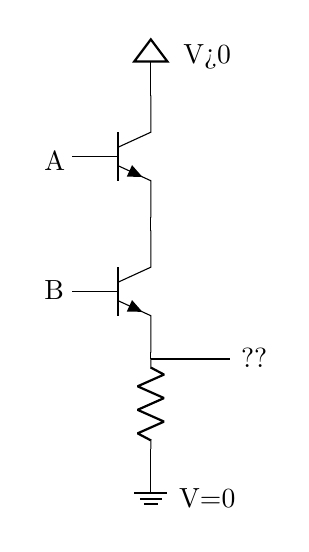
\begin{tikzpicture}
				% Paths, nodes and wires:
				\node[ground] at (1, 4.286){};
				\node[sground, yscale=-1] at (1, 9){};
				\node[shape=rectangle, minimum width=1.197cm, minimum height=0.679cm] at (1.812, 9.429){} node[anchor=north west, align=left, text width=0.809cm, inner sep=6pt] at (1.196, 9.786){V>0};
				\node[shape=rectangle, minimum width=0.608cm, minimum height=0.536cm] at (1.464, 3.857){} node[anchor=north west, align=left, text width=0.22cm, inner sep=6pt] at (1.143, 4.143){V=0};
				\node[npn] at (1, 8.143){};
				\node[npn] at (1, 6.429){};
				\draw (1, 5.571) to[american resistor, /tikz/circuitikz/bipoles/length=1.12cm] (1, 4.429);
				\draw (1, 9) -- (1, 8.913);
				\draw (1, 7.373) -- (1, 7.199);
				\draw (1, 5.659) -- (1, 5.571);
				\draw (1, 4.429) -- (1, 4.286);
				\draw (1, 5.571) -- (2, 5.571);
				\draw (0.16, 6.429) -- (0, 6.429);
				\draw (0.16, 8.143) -- (0, 8.143);
				\node[shape=rectangle, minimum width=0.679cm, minimum height=0.679cm] at (-0.214, 8.071){} node[anchor=north west, align=left, text width=0.291cm, inner sep=6pt] at (-0.571, 8.429){A};
				\node[shape=rectangle, minimum width=0.679cm, minimum height=0.679cm] at (-0.214, 6.429){} node[anchor=north west, align=left, text width=0.291cm, inner sep=6pt] at (-0.571, 6.786){B};
				\node[shape=rectangle, minimum width=0.679cm, minimum height=0.679cm] at (2.286, 5.571){} node[anchor=north west, align=left, text width=0.291cm, inner sep=6pt] at (1.929, 5.929){??};
			\end{tikzpicture}
		\end{column}
	\end{columns}
\end{frame}




\Subsection{Resistors}



\begin{frame}{What is a resistor?}
	light bulb

	ceramic

	the coils in your toaster

	something to soak up energy

	if you run electric current through it and it gets hot, it's a resistor (or at least has resistance)
\end{frame}


\begin{frame}{Voltage Drops in the Resistor}
	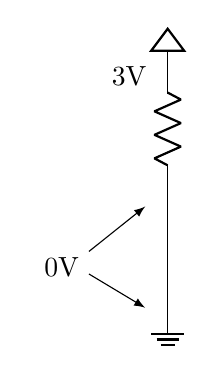
\begin{tikzpicture}
		% Paths, nodes and wires:
		\node[ground] at (2.571, 5.659){};
		\draw (2.571, 8.484) to[american resistor, /tikz/circuitikz/bipoles/length=1.12cm] (2.571, 7.199);
		\node[sground, yscale=-1] at (2.571, 8.484){};
		\node[shape=rectangle, minimum width=0.608cm, minimum height=0.536cm] at (1.964, 8.571){} node[anchor=north west, align=left, text width=0.22cm, inner sep=6pt] at (1.643, 8.857){3V};
		\node[shape=rectangle, minimum width=0.608cm, minimum height=0.536cm] at (1.107, 6.143){} node[anchor=north west, align=left, text width=0.22cm, inner sep=6pt] at (0.786, 6.429){0V};
		\draw[-latex] (1.571, 6.286) -- (2.286, 6.857);
		\draw[-latex] (1.571, 6) -- (2.286, 5.571);
		\draw (2.571, 7.199) -- (2.571, 5.659);
	\end{tikzpicture}
\end{frame}




\begin{frame}{Voltage only drops if it has somewhere to go}

Voltage drop only happens if electricity is flowing. Otherwise the voltage is the same everywhere

	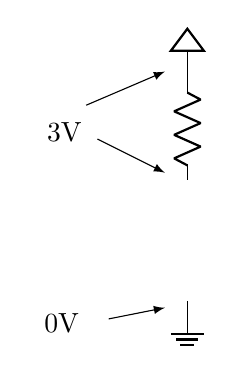
\begin{tikzpicture}
		% Paths, nodes and wires:
		\node[ground] at (2.571, 5.659){};
		\draw (2.571, 8.484) to[american resistor, /tikz/circuitikz/bipoles/length=1.12cm] (2.571, 7.199);
		\node[sground, yscale=-1] at (2.571, 8.484){};
		\node[shape=rectangle, minimum width=0.608cm, minimum height=0.536cm] at (0.893, 7.857){} node[anchor=north west, align=left, text width=0.22cm, inner sep=6pt] at (0.571, 8.143){3V};
		\node[shape=rectangle, minimum width=0.608cm, minimum height=0.536cm] at (0.857, 5.429){} node[anchor=north west, align=left, text width=0.22cm, inner sep=6pt] at (0.536, 5.714){0V};
		\draw[-latex] (1.286, 8.143) -- (2.286, 8.571);
		\draw[-latex] (1.429, 7.714) -- (2.286, 7.286);
		\draw[-latex] (1.571, 5.429) -- (2.286, 5.571);
	\end{tikzpicture}
\end{frame}


\begin{frame}{NOT ALLOWED}
	\begin{columns}
		\begin{column}{0.5\textwidth}
			We assume:
			\begin{itemize}
				\item Top rail fixed at V>0
				\item Bottom rail fixed at 0V
				\item Wires have zero resistance
			\end{itemize}
		\end{column}
		\begin{column}{0.5\textwidth}
			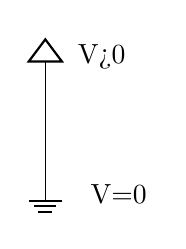
\begin{tikzpicture}
				% Paths, nodes and wires:
				\node[ground] at (1, 8){};
				\node[sground, yscale=-1] at (1, 9){};
				\node[shape=rectangle, minimum width=1.197cm, minimum height=0.679cm] at (1.813, 9.429){} node[anchor=north west, align=left, text width=0.809cm, inner sep=6pt] at (1.196, 9.786){V>0};
				\node[shape=rectangle, minimum width=0.608cm, minimum height=0.536cm] at (1.679, 7.714){} node[anchor=north west, align=left, text width=0.22cm, inner sep=6pt] at (1.357, 8){V=0};
				\draw (1, 9) -- (1, 8);
			\end{tikzpicture}		\end{column}
	\end{columns}

	If you try to build this, one of those assumptions will fail. What might that look like?

\end{frame}


\Subsection{Transistors}

\begin{frame}{Historical Transistors}
	\includegraphics[width=0.5\columnwidth]{images/tube-transistor-wiki}
\end{frame}


\begin{frame}{Modern Transistors}
	\includegraphics[width=\columnwidth]{images/semiconductor-transistor-overkill}
\end{frame}



\begin{frame}{Transistor Behavior}

	https://www.101computing.net/creating-logic-gates-using-transistors/

	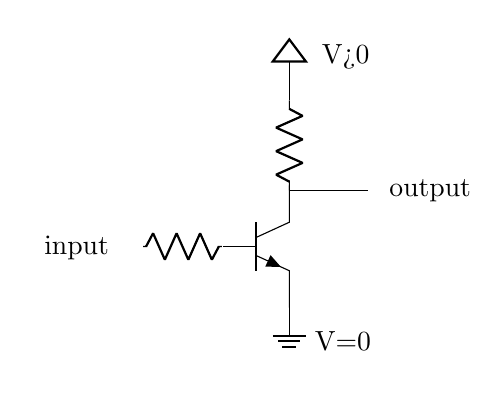
\begin{tikzpicture}
		% Paths, nodes and wires:
		\node[ground] at (1, 6.286){};
		\node[sground, yscale=-1] at (1, 9){};
		\node[shape=rectangle, minimum width=1.197cm, minimum height=0.679cm] at (1.813, 9.429){} node[anchor=north west, align=left, text width=0.809cm, inner sep=6pt] at (1.196, 9.786){V>0};
		\node[shape=rectangle, minimum width=0.608cm, minimum height=0.536cm] at (1.429, 5.857){} node[anchor=north west, align=left, text width=0.22cm, inner sep=6pt] at (1.107, 6.143){V=0};
		\draw (1, 8.857) to[american resistor, /tikz/circuitikz/bipoles/length=1.12cm] (1, 7.714);
		\draw (1, 9) -- (1, 8.857);
		\draw (1, 7.714) -- (2, 7.714);
		\node[shape=rectangle, minimum width=1.197cm, minimum height=0.679cm] at (2.67, 7.714){} node[anchor=north west, align=left, text width=0.809cm, inner sep=6pt] at (2.054, 8.071){output};
		\draw (-0.857, 7) to[american resistor, /tikz/circuitikz/bipoles/length=1.12cm] (0.143, 7);
		\draw (0.286, 7) -- (0.408, 7);
		\node[npn] at (1, 7){};
		\node[shape=rectangle, minimum width=1.197cm, minimum height=0.679cm] at (-1.714, 7){} node[anchor=north west, align=left, text width=0.809cm, inner sep=6pt] at (-2.33, 7.357){input};
	\end{tikzpicture}
\end{frame}


\begin{frame}{Transistor Behavior}
	\begin{columns}
		\begin{column}{0.5\textwidth}
			\usetikzlibrary{shapes.geometric}
			\begin{tikzpicture}
				% Paths, nodes and wires:
				\node[ground] at (1, 6.286){};
				\node[sground, yscale=-1] at (1, 9){};
				\node[shape=rectangle, minimum width=1.197cm, minimum height=0.679cm] at (1.813, 9.429){} node[anchor=north west, align=left, text width=0.809cm, inner sep=6pt] at (1.196, 9.786){V>0};
				\node[shape=rectangle, minimum width=0.608cm, minimum height=0.536cm] at (1.429, 5.857){} node[anchor=north west, align=left, text width=0.22cm, inner sep=6pt] at (1.107, 6.143){V=0};
				\draw (1, 8.857) to[american resistor, /tikz/circuitikz/bipoles/length=1.12cm] (1, 7.714);
				\node[shape=ellipse, draw, line width=1pt, dash pattern={on 1pt off 2pt}, minimum width=1.149cm, minimum height=1.108cm] at (1, 7){};
				\node[shape=rectangle, minimum width=1.197cm, minimum height=0.965cm] at (-1.33, 7.143){} node[anchor=north west, align=left, text width=0.809cm, inner sep=6pt] at (-1.946, 7.643){input\\V>0};
				\draw (1, 6.571) to[cute closed switch] (1, 7.429);
				\draw (1, 9) -- (1, 8.857);
				\draw (1, 7.714) -- (1, 7.429);
				\draw (1, 6.571) -- (1, 6.286);
				\draw (1, 7.714) -- (2, 7.714);
				\node[shape=rectangle, minimum width=1.197cm, minimum height=0.679cm] at (2.67, 7.714){} node[anchor=north west, align=left, text width=0.809cm, inner sep=6pt] at (2.054, 8.071){??};
				\draw (-0.714, 7) to[american resistor, /tikz/circuitikz/bipoles/length=1.12cm] (0.286, 7);
				\draw (0.286, 7) -- (0.408, 7);
			\end{tikzpicture}
		\end{column}
		\begin{column}{0.5\textwidth}
			\usetikzlibrary{shapes.geometric}
			\begin{tikzpicture}
				% Paths, nodes and wires:
				\node[ground] at (1, 6.286){};
				\node[sground, yscale=-1] at (1, 9){};
				\node[shape=rectangle, minimum width=1.197cm, minimum height=0.679cm] at (1.813, 9.429){} node[anchor=north west, align=left, text width=0.809cm, inner sep=6pt] at (1.196, 9.786){V>0};
				\node[shape=rectangle, minimum width=0.608cm, minimum height=0.536cm] at (1.429, 5.857){} node[anchor=north west, align=left, text width=0.22cm, inner sep=6pt] at (1.107, 6.143){V=0};
				\draw (1, 8.857) to[american resistor, /tikz/circuitikz/bipoles/length=1.12cm] (1, 7.714);
				\node[shape=ellipse, draw, line width=1pt, dash pattern={on 1pt off 2pt}, minimum width=1.149cm, minimum height=1.108cm] at (1, 7){};
				\node[shape=rectangle, minimum width=1.197cm, minimum height=0.965cm] at (-1.33, 7.143){} node[anchor=north west, align=left, text width=0.809cm, inner sep=6pt] at (-1.946, 7.643){input\\V=0};
				\draw (1, 6.571) to[cute open switch] (1, 7.429);
				\draw (1, 9) -- (1, 8.857);
				\draw (1, 7.714) -- (1, 7.429);
				\draw (1, 6.571) -- (1, 6.286);
				\draw (1, 7.714) -- (2, 7.714);
				\node[shape=rectangle, minimum width=1.197cm, minimum height=0.679cm] at (2.67, 7.714){} node[anchor=north west, align=left, text width=0.809cm, inner sep=6pt] at (2.054, 8.071){??};
				\draw (-0.714, 7) to[american resistor, /tikz/circuitikz/bipoles/length=1.12cm] (0.286, 7);
				\draw (0.286, 7) -- (0.408, 7);
			\end{tikzpicture}
		\end{column}
	\end{columns}
\end{frame}


\begin{frame}{Transistor Behavior}
	\begin{columns}
		\begin{column}{0.5\textwidth}
			\usetikzlibrary{shapes.geometric}
			\begin{tikzpicture}
				% Paths, nodes and wires:
				\node[ground] at (1, 6.286){};
				\node[sground, yscale=-1] at (1, 9){};
				\node[shape=rectangle, minimum width=1.197cm, minimum height=0.679cm] at (1.813, 9.429){} node[anchor=north west, align=left, text width=0.809cm, inner sep=6pt] at (1.196, 9.786){V>0};
				\node[shape=rectangle, minimum width=0.608cm, minimum height=0.536cm] at (1.429, 5.857){} node[anchor=north west, align=left, text width=0.22cm, inner sep=6pt] at (1.107, 6.143){V=0};
				\draw (1, 8.857) to[american resistor, /tikz/circuitikz/bipoles/length=1.12cm] (1, 7.714);
				\node[shape=ellipse, draw, line width=1pt, dash pattern={on 1pt off 2pt}, minimum width=1.149cm, minimum height=1.108cm] at (1, 7){};
				\node[shape=rectangle, minimum width=1.197cm, minimum height=0.965cm] at (-1.33, 7.143){} node[anchor=north west, align=left, text width=0.809cm, inner sep=6pt] at (-1.946, 7.643){input\\V>0};
				\draw (1, 6.571) to[cute closed switch] (1, 7.429);
				\draw (1, 9) -- (1, 8.857);
				\draw (1, 7.714) -- (1, 7.429);
				\draw (1, 6.571) -- (1, 6.286);
				\draw (1, 7.714) -- (2, 7.714);
				\node[shape=rectangle, minimum width=1.197cm, minimum height=0.679cm] at (2.67, 7.714){} node[anchor=north west, align=left, text width=0.809cm, inner sep=6pt] at (2.054, 8.071){output\\V=0};
				\draw (-0.714, 7) to[american resistor, /tikz/circuitikz/bipoles/length=1.12cm] (0.286, 7);
				\draw (0.286, 7) -- (0.408, 7);
			\end{tikzpicture}
		\end{column}
		\begin{column}{0.5\textwidth}
			\usetikzlibrary{shapes.geometric}
			\begin{tikzpicture}
				% Paths, nodes and wires:
				\node[ground] at (1, 6.286){};
				\node[sground, yscale=-1] at (1, 9){};
				\node[shape=rectangle, minimum width=1.197cm, minimum height=0.679cm] at (1.813, 9.429){} node[anchor=north west, align=left, text width=0.809cm, inner sep=6pt] at (1.196, 9.786){V>0};
				\node[shape=rectangle, minimum width=0.608cm, minimum height=0.536cm] at (1.429, 5.857){} node[anchor=north west, align=left, text width=0.22cm, inner sep=6pt] at (1.107, 6.143){V=0};
				\draw (1, 8.857) to[american resistor, /tikz/circuitikz/bipoles/length=1.12cm] (1, 7.714);
				\node[shape=ellipse, draw, line width=1pt, dash pattern={on 1pt off 2pt}, minimum width=1.149cm, minimum height=1.108cm] at (1, 7){};
				\node[shape=rectangle, minimum width=1.197cm, minimum height=0.965cm] at (-1.33, 7.143){} node[anchor=north west, align=left, text width=0.809cm, inner sep=6pt] at (-1.946, 7.643){input\\V=0};
				\draw (1, 6.571) to[cute open switch] (1, 7.429);
				\draw (1, 9) -- (1, 8.857);
				\draw (1, 7.714) -- (1, 7.429);
				\draw (1, 6.571) -- (1, 6.286);
				\draw (1, 7.714) -- (2, 7.714);
				\node[shape=rectangle, minimum width=1.197cm, minimum height=0.679cm] at (2.67, 7.714){} node[anchor=north west, align=left, text width=0.809cm, inner sep=6pt] at (2.054, 8.071){output\\V>0};
				\draw (-0.714, 7) to[american resistor, /tikz/circuitikz/bipoles/length=1.12cm] (0.286, 7);
				\draw (0.286, 7) -- (0.408, 7);
			\end{tikzpicture}
		\end{column}
	\end{columns}
\end{frame}



\begin{frame}{Why two resistors?}

In many cases, we can get away with just one resistor. The previous example had two. Why?

Always need a resistor between a voltage source and ground. Transistors have internal resistance but it's very small. Easy to burn them out

\end{frame}





\begin{frame}{More Complex Example}
	\begin{tikzpicture}
		% Paths, nodes and wires:
		\node[ground] at (1, 4.286){};
		\node[sground, yscale=-1] at (1, 9){};
		\node[shape=rectangle, minimum width=1.197cm, minimum height=0.679cm] at (1.813, 9.429){} node[anchor=north west, align=left, text width=0.809cm, inner sep=6pt] at (1.196, 9.786){V>0};
		\node[shape=rectangle, minimum width=0.608cm, minimum height=0.536cm] at (1.679, 4){} node[anchor=north west, align=left, text width=0.22cm, inner sep=6pt] at (1.357, 4.286){V=0};
		\draw (1, 5.571) to[american resistor, /tikz/circuitikz/bipoles/length=1.12cm] (1, 4.429);
		\node[npn] at (1, 8.143){};
		\node[npn] at (1, 6.429){};
		\draw (1, 9) -- (1, 8.913);
		\draw (1, 7.373) -- (1, 7.199);
		\draw (1, 5.659) -- (1, 5.571);
		\draw (1, 5.571) -- (2, 5.571);
		\draw (0.16, 8.143) -- (0, 8.143);
		\draw (0.16, 6.429) -- (0, 6.429);
		\draw (1, 4.429) -- (1, 4.286);
		\node[shape=rectangle, minimum width=0.668cm, minimum height=0.65cm] at (-0.22, 8.143){} node[anchor=north west, align=left, text width=0.28cm, inner sep=6pt] at (-0.571, 8.485){A};
		\node[shape=rectangle, minimum width=0.668cm, minimum height=0.65cm] at (-0.286, 6.429){} node[anchor=north west, align=left, text width=0.28cm, inner sep=6pt] at (-0.637, 6.771){B};
		\node[shape=rectangle, minimum width=0.668cm, minimum height=0.65cm] at (2.286, 5.628){} node[anchor=north west, align=left, text width=0.28cm, inner sep=6pt] at (1.934, 5.971){??};
	\end{tikzpicture}
\end{frame}




% what is a transistor
% building logic gates

% TEST 3 TOPICS

\Section{Instruction Pipelining}

\Subsection{FDEW Cycle}

\Subsection{Pipelining}

\Subsection{Hazards}

% pipelining
% data hazards
% control hazards

\Section{Assembly Conditionals and Loops}

% b, beq, bne, ...
% if/else
% while loops
% for loops

\input{sections/multiprocessing.tex}
% booting
% forking
% threads, cores, processes
% async


\Section{Appendix}


\Subsection{Raspberry Pi Setup}


\begin{frame}{Pi Setup: Kit Contents}
	\begin{columns}
		\begin{column}{0.5\textwidth}
			\begin{enumerate}
				\item Pi case
				\item Raspberry Pi (in box)
				\item Heat sinks
				\item Power cord
				\item Ethernet to USB adapter
				\item Ethernet cord
				\item USB 2 to USB 3 adapter
				\item SD Card
				\item Accessory case
			\end{enumerate}
		\end{column}
		\begin{column}{0.5\textwidth}
			\includegraphics[width=\columnwidth]{images/pi-kit-contents}
		\end{column}
	\end{columns}
\end{frame}


\begin{frame}{Pi Setup: Apply Heat Sinks}
	\begin{columns}
		\begin{column}{0.5\textwidth}
			\includegraphics[width=\columnwidth]{images/pi-heat-sinks-1}
		\end{column}
		\begin{column}{0.5\textwidth}
			\includegraphics[width=\columnwidth]{images/pi-heat-sinks-2}
		\end{column}
	\end{columns}
\end{frame}

\begin{frame}{Pi Setup: Apply Nonslip Nubs}
	\includegraphics[width=\columnwidth]{images/pi-case-nubs}
\end{frame}

\begin{frame}{Pi Setup: Install in Case}
	\includegraphics[width=\columnwidth]{images/pi-in-case}
\end{frame}

\begin{frame}{Pi Setup: SD Card}
	\begin{columns}
		\begin{column}{0.5\textwidth}
			\includegraphics[width=\columnwidth]{images/pi-sd-card-1}
		\end{column}
		\begin{column}{0.5\textwidth}
			\includegraphics[width=\columnwidth]{images/pi-sd-card-2}
		\end{column}
	\end{columns}
\end{frame}

\begin{frame}{Pi Setup: Connect to Laptop}
	\includegraphics[width=\columnwidth]{images/pi-to-laptop}
\end{frame}

\begin{frame}{Pi Setup: Connect to Power}
\end{frame}

\begin{frame}{Laptop Setup: Enable WiFi}
	\includegraphics[width=\columnwidth]{images/pi-network-settings}
\end{frame}

\begin{frame}{Laptop Setup: Install VSCode}
	\includegraphics[width=\columnwidth]{images/vscode-remote-ssh}
\end{frame}

\begin{frame}{Laptop Setup: Add Remote Connection}
	\includegraphics[width=\columnwidth]{images/vscode-add-remote}
\end{frame}

\begin{frame}{Laptop Setup: SSH Login}
	\begin{itemize}
		\item Default username/password is raspberri/pi
		\item Make sure to update username and password
	\end{itemize}
\end{frame}


\Subsection{CSGit Setup}

% vscode setup
% pi setup
% csgit setup


\end{document}
% booting
% forking
% threads, cores, processes
% async


\documentclass{beamer}
\usepackage[utf8]{inputenc}
\usepackage[T1]{fontenc}
\usepackage{circuitikz}

\usepackage{multirow}

\title{CS241: Hardware Design}
\date{\today}
\author[Fyfe and Lynn]{Charles Fyfe and Melissa Lynn}
\institute{St Olaf College}

\usetheme{grape}

\usepackage{parskip}
\usepackage{multicol}
\usepackage{graphicx}
% make \oplus look nice
\usepackage{amssymb}

\begin{document}


\titlepage

% just sections up top
\setcounter{tocdepth}{1}

\begin{frame}{Outline}

	\begin{multicols*}{2}
		\tableofcontents
	\end{multicols*}
\end{frame}

% show subsections later
\setcounter{tocdepth}{2}


\Section{Syllabus}

\begin{frame}{Course Overview}

	\includegraphics[width=\columnwidth]{images/dune-robot-hbo}

	{\center
		Thou shalt not make a machine in the likeless of a human mind
	}

	{\small \hfill
		The Orange Catholic Bible, Dune, Frank Herbert
	}
\end{frame}


\begin{frame}{Course Overview}

	Computers feel like magic. You type words. The machine does complex things. Especially in the era of large language models

	But it's not magic. Computers are made of semiconductors, metal, and magnets. Three different kinds of rocks

	This course is about demystifying the machine and exploring how, fundamentally, computers do what they do. Specifically, we'll be looking at:
	\begin{itemize}
		\item The fundamental components of a computer
		\item How data is stored on a computer
		\item Building electrical circuits to perform logic
		\item Programming in Assembly (a very low-level language)
	\end{itemize}
\end{frame}

\Subsection{Grading}

\begin{frame}{Course Grade Breakdown}
	\begin{itemize}
		\item Quizzes and final: 45\%
		\item Homework and labs: 45\%
		\item Participation: 10\%
	\end{itemize}
\end{frame}

\begin{frame}{Standards-Based Grading}
	\begin{itemize}
		\item There are nine standards in the class. Each is worth 5\% of your grade.
		\item There are three quizzes. Each quiz covers three standards.
		\item The final covers all nine standards.
		\item If you demonstrate proficiency on the quiz, you're done with that standard. Full credit. You can skip that part of the final.
		\item If you demonstrate partial proficiency on the quiz, you get half credit. Try again on the final for full credit.
		\item If you do not demonstrate proficiency on the quiz, you get no credit. You can still get full credit on the final!
	\end{itemize}
\end{frame}


\begin{frame}{Homework and Labs}
	\begin{itemize}
		\item One or more lab exercises for each standard. We start these together in class. You may need to finish on your own time.
		\item We will have a homework assignment for each standard.
		\item Please work together in small groups.
		\item Please ensure that the work you turn in reflects your own understanding.
	\end{itemize}
\end{frame}

\begin{frame}{Late Work Policy}
	Please try to get your work in on time.
	\begin{itemize}
		\item If you don't get your work done on time, you may fall behind in the class.
		\item Late work is inconvenient for the TAs. They will be grumpy and vindictive when they grade your work.
		\item TAs will have their own finals to worry about! Late work at the end of the semester might be refused.
	\end{itemize}
	If you need an extension, please reach out beforehand.
\end{frame}

\begin{frame}{Peer Reviews}
	\begin{itemize}
		\item Participation score (10\% of your total grade) is mostly based on peer reviews.
		\item Reviews will be short. Less than one page.
		\item You can get full credit here without too much trouble. Show up. Work together. Make it easy for your peers to say nice things about you.
		\item I recommend keeping notes over the course of the semester when someone is particularly helpful, insightful, etc. Good reviews have concrete examples.
	\end{itemize}
\end{frame}

\Subsection{Office Hours}

\begin{frame}{Office Hours}
	TODO
\end{frame}


\Subsection{Disability Accommodations}

\begin{frame}{Disability Accommodations}
	I am committed to supporting the learning of all students in my class. If you have already
	registered with Disability and Access (DAC) and have your letter of accommodations, please
	meet with me as soon as possible to discuss, plan, and implement your accommodations in the
	course. If you have or think you have a disability (learning, sensory, physical, chronic health,
	mental health or attentional), please contact Disability and Access staff at 507-786-3288 or by visiting \href{https://wp.stolaf.edu/academic-support/dac}{their website}.


	If you have an accommodation that allows you extra time or a low distraction environment for
	quizzes and exams, please email me at least three days before each quiz or exam, so that I can
	make sure to reserve a room.
\end{frame}


\Subsection{Religious Accommodations}

\begin{frame}{Religious Accommodations}
	As part of my commitment to make St Olaf an inclusive community, I will provide students with
	reasonable religious accommodations. If you will be missing class for a religious observance or
	require another religious accommodation, please meet with me to discuss these.
\end{frame}


\Subsection{Academic Integrity}

\begin{frame}{Academic Integrity}

	Plagiarism is a serious academic offense. Hand in your own work. Give credit appropriately when you draw from the work of others. For more information please see:

	\begin{itemize}
		\item \href{https://wp.stolaf.edu/facultyhandbook/academic-integrity-faculty-handbook-category-2}{Faculty Handbook: Academic Integrity}
		\item \href{https://wp.stolaf.edu/honorcouncil/}{The Honor Code}
		\item \href{https://wp.stolaf.edu/roadmap-to-academic-integrity}{Roadmap to Academic Integrity}
	\end{itemize}

	Work that violates this policy will typically receive no credit. In especially serious cases the penalty can be an F in the course.
\end{frame}

\Subsection{AI Use Policy}

\begin{frame}{AI Usage Policy}
	Please not submit AI work as your own.

	You may use AI tools when studying, but be careful. These tools are very good with mainstream languages like Python. We're working with Assembly, which is very much \textbf{not} a mainstream language.

\end{frame}


\Subsection{St Olaf Land Acknowledgement}

\begin{frame}{St Olaf Land Acknowledgement}
	We stand on the homelands of the Wahpekute Band of the Dakota Nation. We honor with
	gratitude the people who have stewarded the land throughout the generations and their ongoing
	contributions to this region. We acknowledge the ongoing injustices that we have committed
	against the Dakota Nation, and we wish to interrupt this legacy, beginning with acts of healing
	and honest storytelling about this place.

	For more information about land acknowledgement statements at St Olaf, please see \href{https://wp.stolaf.edu/education/land-acknowledgement/}{here} and \href{https://wp.stolaf.edu/equity-inclusion/land-acknowledgement/}{here}.
\end{frame}


\Subsection{Statement of Inclusivity}

\begin{frame}{Statement of Inclusivity}
	In keeping with St. Olaf College's mission statement, this class strives to be an inclusive
	learning community, respecting those of differing backgrounds and beliefs. As a community, we
	aim to be respectful to all citizens in this class, regardless of race, ethnicity, religion, gender or
	sexual orientation.
\end{frame}


\Subsection{Gender Pronouns}

\begin{frame}{Gender Pronouns}
	This course affirms people of all gender expressions and gender identities. If you go by a
	different name than what is on the class roster, please let me know.

	Using correct gender
	pronouns is important to me, so you are encouraged to share your pronouns with me and
	correct me if a mistake is made. If you have any questions or concerns, please do not hesitate
	to contact me.
\end{frame}


\Subsection{Multilingual Student Support}

\begin{frame}{Multilingual Student Support}
	I am committed to making course content accessible to all students. If English is not your first
	language and this causes you concern about the course, please speak with me. Students who
	would like extra support with writing or speaking in English can also contact the language support specialist (\href{mailto:berryag@stolaf.edu}{berryag@stolaf.edu}) in the Academic Success Center.
\end{frame}


\Subsection{Mental Health}

\begin{frame}{Mental Health}

	I greatly value your experience in this class, and it is my duty to facilitate a safe, caring, and
	productive learning environment.

	I recognize that you may experience a range of emotional, physical, and/or psychological
	issues, both in and out of the classroom, that may distract you from your learning.

	If you are experiencing such issues, please do not hesitate to come see me. I am here to listen.
	We can also discuss what further resources might be available to you.
\end{frame}

\Subsection{Required Referrals}


\begin{frame}{Required Referrals}
	You are welcome to talk to me about circumstances outside the course that
	affect your classroom experience or acadmic performance. However, please keep
	in mind that I am required to refer cases of discrimination, harassment,
	sexual misconduct, and violence.

	Here are some resources where you can share privately:

	\begin{itemize}
		\item Boe House Counseling Center
		\item College Pastors and Chaplains
		\item Sexual Assault Resource Network (SARN)
		\item Health Services
		\item TimelyCare
	\end{itemize}
\end{frame}




\Subsection{St. Olaf Pride Statement}

\begin{frame}{St. Olaf Pride Statement}
	As an Ole, I will practice:
	\begin{itemize}
		\item Passion for learning and pursuit of vocation
		\item Respect for the worth and dignity of all people
		\item Integrity at all times, in all circumstances
		\item Dedication to a life of service, and
		\item Engagement with my community and the world.
	\end{itemize}
\end{frame}









\Subsection{Important Links}

\begin{frame}{Important Links}
	\begin{itemize}
		\item ARM tutorial https://computerscience.chemeketa.edu/armTutorial/index.html
		\item ARM simulator https://cpulator.01xz.net/?sys=arm
		\item circuit simulator: https://circuitverse.org/simulator
	\end{itemize}
\end{frame}





% TEST 1 TOPICS


\Section{Data Representation}

\begin{frame}{How do computers store information?}
	Computers work using electrical signals which can be on or off. If we let:
	\begin{itemize}
		\item On means 1
		\item Off means 0
	\end{itemize}
	We can use sequences of 0s and 1s to represent information
\end{frame}

\Subsection{Positive Integers in Binary}

\begin{frame}{Numbers in Base Ten (aka Decimal)}
	Let's start by talking about how we write numbers normally.

	For example, let's look at the number 109:
	\begin{align*}
		109 & = 100 \;+\; 0 \;+\; 9                                   \\
		    & = 1 \Times 10^2 \;+\; 0 \Times 10^1 \;+\; 9 \Times 10^0
	\end{align*}
	This way of writing numbers is called base ten.
	We use ten digits (0 to 9 inclusive) and each position in the number is scaled by a power of ten.

	In terms of math, there is nothing special about base ten. We probably use it
	because we have ten fingers. Some ancient civilizations used sompletely
	different systems for counting!
\end{frame}

\begin{frame}{Numbers in Base Two (aka Binary)}
	Computers don't have fingers. They express everything as sequences of 1s and 0s. This format is called binary:

	\begin{align*}
		0b1101101 & =
		1 \Times 2^6 +
		1 \Times 2^5 +
		0 \Times 2^4 +
		1 \Times 2^3 +
		1 \Times 2^2 +
		0 \Times 2^1 +
		1 \Times 2^0                              \\
		          & = 64 + 32 + 0 + 8 + 4 + 0 + 1 \\
		          & = 109                         \\
	\end{align*}
	Importantly: we always use the prefix ``0b'' to avoid confusion when writing numbers in binary.

	1101 is one thousand one hundred and one

	0b1101 is thirteen
\end{frame}

\begin{frame}{Converting from Decimal to Binary}

	If the number is odd, append a 1 on the left. Otherwise, append a 0. Then
	divide your decimal number by two and ignore any remainder. Repeat until your
	decimal number is zero. \\

	For example, starting with 58:

	\begin{itemize}
		\item 58 is even, so append \Highlight{0}. Divide by two, leaving 29.
		\item 29 is odd, so append \Highlight{1}0. Divide by two, leaving 14.
		\item 14 is even, so append \Highlight{0}10. Divide by two, leaving 7.
		\item 7 is odd, so append \Highlight{1}010. Divide by two, leaving 3.
		\item 3 is odd, so append \Highlight{1}1010. Divide by two, leaving 1.
		\item 1 is odd, so append \Highlight{1}11010. Divide by two, leaving 0.
	\end{itemize}

	So 58 in binary is 0b111010.

\end{frame}

\begin{frame}{Converting from Binary to Decimal}

	We can confirm by converting back. The rightmost bit is worth 1, then 2, then
	4, and so on:

	\begin{align*}
		0b111010 & =
		1 \Times 2^5 +
		1 \Times 2^4 +
		1 \Times 2^3 +
		0 \Times 2^2 +
		1 \Times 2^1 +
		0 \Times 2^0                          \\
		         & = 32 + 16  + 8 + 0 + 2 + 0 \\
		         & = 58
	\end{align*}

\end{frame}

\begin{frame}{Addition in Binary}
	Binary addition works just like decimal addition.
	Start from the right, add straight down, and carry when you run out of digits.

	For example:
	\[
		\begin{array}{ccccccccc}
			1 & 1 & 1 & 1 & 1 &   &   &   &   \\
			  & 0 & 0 & 1 & 1 & 1 & 0 & 0 & 0 \\
			+ & 1 & 1 & 1 & 0 & 1 & 0 & 0 & 1 \\
			\hline
			1 & 0 & 0 & 1 & 0 & 0 & 0 & 0 & 1 \\
		\end{array}
	\]

	What happens if we try to perform this operation but we only have 8 bits to
	store the answer?
\end{frame}

\begin{frame}{Multiplication in Binary}
	Binary multiplication works just like decimal multiplication.
	Multiply the top number by the rightmost digit of the bottom number.
	Then move to the next line, add a zero, and repeat for the next digit.
	Finally, add up the lines. For example:
	\[
		\begin{array}{cccccc}
			  &   &        & 1 & 1 & 0 \\
			  &   & \times & 1 & 0 & 1 \\
			\hline
			  &   &        & 1 & 1 & 0 \\
			  &   & 0      & 0 & 0 & 0 \\
			+ & 1 & 1      & 0 & 0 & 0 \\
			\hline
			  & 1 & 1      & 1 & 1 & 0 \\
		\end{array}
	\]
\end{frame}

\begin{frame}{Division in Binary}
	To divide by 2, shift the bits one place to the right. \\

	To divide by 4, shift the bits two places to the right. \\

	That's about as deep as we go in this class. If you're curious to learn more,
	see the textbook.

\end{frame}



\Subsection{Hexadecimal}

\begin{frame}{What? Why?}

	Binary is how machines store data. But writing out binary by hand is a chore.
	In practice, it's often convenient to use hexadecimal (base 16) instead.

	\begin{itemize}
		\item Decimal uses ten digits, 0-9
		\item Binary uses two digits, 0 and 1
		\item Hexadecimal uses sixteen digits: 0-9 along with A-F
	\end{itemize}
	Hexadecimal values are always prefixed with ``0x'' to avoid ambiguity.
\end{frame}

\begin{frame}{Converting Between Binary and Hexadecimal}

	Converting back and forth between binary and hexadecimal does not require any
	math! Every four bits become one hex digit.
	\begin{align*}
		0b0000 & = 0x0 = 0 & 0b1000 & = 0x8 = 8  \\
		0b0001 & = 0x1 = 1 & 0b1001 & = 0x9 = 9  \\
		0b0010 & = 0x2 = 2 & 0b1010 & = 0xA = 10 \\
		0b0011 & = 0x3 = 3 & 0b1011 & = 0xB = 11 \\
		0b0100 & = 0x4 = 4 & 0b1100 & = 0xC = 12 \\
		0b0101 & = 0x5 = 5 & 0b1101 & = 0xD = 13 \\
		0b0110 & = 0x6 = 6 & 0b1110 & = 0xE = 14 \\
		0b0111 & = 0x7 = 7 & 0b1111 & = 0xF = 15 \\
	\end{align*}
\end{frame}

\begin{frame}{Converting Hexadecimal to Decimal}

	Hexadecimal is base 16. So each place corresponds to a power of 16.

	\begin{align*}
		0x3AB & = 3 \times 16^2 + 10 \times 16^1 + 11 \times 16^0 \\
		      & = 3 \times 256 + 10 \times 16 + 11 \times 1       \\
		      & = 768 + 160 + 11                                  \\
		      & = 954                                             \\
	\end{align*}

	Hexadecimal is very compact! These numbers get big fast

\end{frame}

\begin{frame}{Arithmetic in Hexadecimal}

	Addition and multiplication work in hexadecimal just like they do in binary and
	decimal. Just be careful about carrying.

	\[
		\begin{array}{ccccc}
			1 &   &   & 1 &   \\
			  & 4 & 1 & 7 & B \\
			+ & C & 2 & 0 & F \\
			\hline
			1 & 0 & 3 & 8 & A \\
		\end{array}
	\]

\end{frame}






\Subsection{Negatives in Binary}

\begin{frame}{First Attempt: Signed Magnitude}

	We can use the first digit to hold the sign, then the rest of the digits to
	hold magnitue:

	\begin{itemize}
		\item 0b\Highlight{0}1011001 is positive 10110001, so 89
		\item 0b\Highlight{1}1011001 is negative 1011001, so -89
	\end{itemize}

	This is nice and straightforward!

\end{frame}

\begin{frame}{Addition and Subtraction with Signed Magnitude}
	Adding positive numbers works just the same. But what happens if we throw a minus sign in there?

	For example, let's look at 12 - 5. First, rewrite it as 12 + (-5). Then:

	\[
		\begin{array}{ccccccccc}
			  & 0 & 0 & 0 & 0 & 1 & 1 & 0 & 0 \\
			+ & 1 & 0 & 0 & 0 & 0 & 1 & 0 & 1 \\
			\hline
			  & ? & ? & ? & ? & ? & ? & ? & ? \\
		\end{array}
	\]

	We know the result should be 7 (0b00000111). But our regular rules for addition
	do not get us there.
\end{frame}

\begin{frame}{Zero with Signed Magnitude}

	Using signed magnitude, 0b00000000 is zero.

	And 0b10000000 is negative zero (which is also zero).

	Using this convention, we have to worry about the difference between numerical
	equality and bitwise equality. That seems pretty messy.
\end{frame}

\begin{frame}{Can We Do Better?}
	Signed magnitude was a swing and a miss. What do we want when we talk about negative numbers?
	\begin{itemize}
		\item We want positive numbers to work like we expect
		\item We want 0b00000000 to be zero, with no ambiguity
		\item We want addition and subtraction to work the same for positive and negative
	\end{itemize}
\end{frame}

\begin{frame}{Another Idea: Two's Complement}
	We know 1 - 1 = 0. Put another way, 1 + (-1) = 0. Can we work backwards from there to figure out how to write -1?
	\[
		\begin{array}{ccccccccc}
			  & 0 & 0 & 0 & 0 & 0 & 0 & 0 & 1 \\
			+ & 1 & 1 & 1 & 1 & 1 & 1 & 1 & 1 \\
			\hline
			  & 0 & 0 & 0 & 0 & 0 & 0 & 0 & 0 \\
		\end{array}
	\]

	Remember: on a computer, our numbers have to fit in a set number of bits.
	Anything past that gets thrown away. This is called overflow. In this case,
	overflow works in our favor!
\end{frame}

\begin{frame}{Working Backwards from Zero}
	We can use the same trick to identify the rest of the negative numbers:
	\begin{itemize}
		\item 0b00000000 is 0
		\item 0b11111111 is -1
		\item 0b11111110 is -2
		\item 0b11111101 is -3
		\item 0b11111100 is -4
		\item etc
	\end{itemize}

\end{frame}

\begin{frame}{The Sign Bit (Again)}
	We only have 256 possible integers. How do we decide where the positives end and the negatives begin?

	Unsigned int: bits are worth 1, 2, 4, 8, 16, 32, 64, 128

	Signed magnitude: bits are worth $\pm1, \pm2, \pm4, \pm8, \pm16, \pm32, \pm64$,
	and the last bit tells us whether to use positive or negative (yikes)

	Two's complement: bits are worth 1, 2, 4, 8, 16, 32, 64, \Highlight{-128}

	Range of possible values is -128 to 127.
\end{frame}

\begin{frame}{Flipping Signs in Two's Complement}
	To flip the sign of a two's complement integer, flip all the bits then add 1. Ignore the overflow (if any). This works for both positive and negative numbers.

	For example:
	\begin{itemize}
		\item 55 is 0b01010111
		\item Flip the bits: 0b10101000, then add 1: 0b10101001
		\item So -55 is 0b10101001
		\item Flip the bits again: 0b01010110, add 1: 0b01010111
		\item So -(-55) = 55 = 0b01010111
	\end{itemize}

	What happens if we negate zero?
\end{frame}

\begin{frame}{Overflow}
	Overflow is important for two's complement. It ensures that positive zero and negative zero are the same. But it is also a constraint!

	Try adding 0b01101001 + 0b01011010:
	\[
		\begin{array}{ccccccccc}
			  &   & 1 & 1 & 1 &   &   &   &   \\
			  & 0 & 1 & 1 & 0 & 1 & 0 & 0 & 1 \\
			+ & 0 & 1 & 0 & 1 & 1 & 0 & 1 & 0 \\
			\hline
			  & 1 & 1 & 0 & 0 & 0 & 0 & 1 & 1 \\
		\end{array}
	\]

	These are two's complement numbers. Convert them to decimal. What just
	happened?

\end{frame}


\Subsection{Fractions and Decimals}

\begin{frame}{The Decimal Point}

	Sometimes we need to store numbers that aren't integers. \\

	Before we worry about binary, what does 21.867 mean? \\

	\begin{align*}
		21.867 & = 2 \Times 10^1 + 1 \Times 10^0 + 8 \Times ?? + 6 \Times ?? + 7 \Times ??
	\end{align*}

\end{frame}

\begin{frame}{The Decimal Point}

	In decimal:
	\begin{align*}
		21.867 & = 2 \Times 10^1 + 1 \Times 10^0 + 8 \Times 10^{-1} + 6 \Times 10^{-2} + 7 \Times 10^{-3}             \\
		       & =2 \Times 10 + 1 \Times 1 + 8 \Times \frac{1}{10} + 6 \Times \frac{1}{100} + 7 \Times \frac{1}{1000} \\
	\end{align*}

	In binary, we can use the same idea:
	\begin{align*}
		0b101.010 & = 1 \Times 2^2 + 0 \Times 2^1 + 1 \Times 2^0 + 0 \Times 2^{-1} + 1 \Times 2^{-2} + 0 \Times 2^{-3} \\
		          & = 1 \Times 4 + 0 + 1 \Times 1 + 0 + 1 \Times \frac{1}{4} + 0                                       \\
		          & = 5.25                                                                                             \\
	\end{align*}

\end{frame}

\begin{frame}{Fixed Point Representation}

	The computer just stores 1s and 0s, not decimal points. How do we distinguish
	these values?
	\begin{itemize}
		\item 0b0101110.1 = 46.5
		\item 0b010111.01 = 23.25
		\item 0b01011.101 = 11.625
	\end{itemize}

	One option is to specify the location of the decimal point ahead of time. For
	example, we could say that our eight-bit binary decimal always has two decimal
	bits. \\

	What is an upside of this approach? What is a downside?

\end{frame}

\begin{frame}{Floating Point Representation}

	Floating point numbers are a bit more complicated, but much more flexible. For
	a 16-bit floating point number we get:

	\begin{itemize}
		\item 1 bit for the sign
		\item 5 bits for the exponent (value -14 to 15)
		\item 10 bits for the significand (value 0 to 1023)
	\end{itemize}

	To turn those components into a value we use:
	\begin{align*}
		\text{value} & = (-1)^{\text{sign}} \times 2^{\text{exponent} - 15} \times \left(1 + \frac{\text{significand}}{1024} \right)
	\end{align*}

	Why offset the exponent?

	Why add 1 to the significand fraction?

\end{frame}

% Explanation here for the 127 offset: https://www.quora.com/Why-do-we-add-127-to-the-exponent-in-IEEE-754-floating-number-format-to-get-the-actual-exponent-value

\begin{frame}{Floating Point Examples}

	\begin{align*}
		\underbrace{0}_\text{sign} \; \underbrace{01111}_\text{exponent} \; \underbrace{0000000000}_\text{significand} & = (-1)^0 \times 2^{15 - 15} \times \left( 1 + \frac{0}{1024} \right) \\
		                                                                                                               & = 1 \times 2^0   \times \left( 1 + 0 \right)                         \\
		                                                                                                               & = 1                                                                  \\
	\end{align*}
	\begin{align*}
		0 \; 01101 \; 0101010101 & = (-1)^0 \times 2^{13 - 15} \times \left( 1 + \frac{341}{1024} \right) \\
		                         & \approx 0.33325195                                                     \\
	\end{align*}
	\begin{align*}
		1 \; 11110 \; 1111111111 & = (-1)^1 \times 2^{30 - 15} \times \left( 1 + \frac{1023}{1024} \right) \\
		                         & = -65504                                                                \\
	\end{align*}

	Why
\end{frame}

\begin{frame}{Floating Point Special Cases}

	\[
		\begin{array}{ccccr}
			0 & 00000 & 0000000000     & = 0          \\
			1 & 00000 & 0000000000     & = -0         \\
			0 & 11111 & 0000000000     & = \infty     \\
			1 & 11111 & 0000000000     & = -\infty    \\
			0 & 11111 & \text{nonzero} & = \text{NaN} \\
		\end{array}
	\]

	There's more to it than this. If you're curious, read up on subnormal numbers
	\href{https://en.wikipedia.org/wiki/Half-precision_floating-point_format}{here}

\end{frame}

\begin{frame}{Floating Point for Big Integers}

	If we're dealing with big numbers, floating point often works better than fixed
	point. This is true even if both formats use the same number of bits.

	\begin{itemize}
		\item 8-bit unsigned integer: max value 255
		\item 16-bit unsigned integer: max value 65,535
		\item 32-bit unsigned integer: max value 4.2 billion % 4,294,967,295
		\item 16-bit floating point: max value 65,504 (also handles negatives, fractions)
		\item 32-bit floating point: max value 340 billion billion billion billion (also handles negatives, fractions)
		      % 340,282,346,638,528,859,811,704,183,484,516,925,440 
	\end{itemize}

\end{frame}

\begin{frame}{Floating Point Limitations}

	So what's the catch?

\end{frame}

%        \item Convert 0b100110.10 from fixed-point binary to decimal.
%        \item Convert 23.75 from decimal to fixed-point binary.
%        \item Add fixed-point binary numbers 0b101101.01 + 0b010011.11. Convert to decimal to confirm your result.
%        \item Show that the 16-bit floating point expression ${1 \; 01000 \; 1100000000}$ is equal to -3.5 in decimal.

\Subsection{Beyond Numbers}

\begin{frame}{What else do computers store?}
	There are many cases where we want a computer to store non-numerical data:
	\begin{itemize}
		\item Text
		\item Colors
		\item Sounds
		\item Images
		\item Videos
		\item Websites
		\item Multiple things at once
	\end{itemize}
\end{frame}

\begin{frame}{Characters and Strings}
	\begin{itemize}
		\item Each character is represented by a number
		\item The most straightforward encoding is ASCII
		\item Modern use cases typically use Unicode (much bigger)
		\item To make a string, put a bunch of characters in a row
		\item Question: how do we identify the end of a string?
	\end{itemize}
\end{frame}

\begin{frame}{ASCII Table}
	\includegraphics[width=\columnwidth]{images/ascii-table}
\end{frame}

\begin{frame}{Colors and Images}
	\begin{itemize}
		\item A color can be described by three numbers (R, G, B)
		\item We can represent an image as a grid of colored pixels
		\item Question: do we need a null byte at the end of a pixel/row/image? Why or why not?
	\end{itemize}
	\includegraphics[width=\columnwidth]{images/mario-pixels}
\end{frame}

\begin{frame}{Sound}
	\begin{itemize}
		\item Sound is pressure vibrations in the air
		\item We can create sound by moving a speaker cone rapidly
		\item To store sound, store the movement of the speaker cone
	\end{itemize}
	\includegraphics[width=0.5\columnwidth]{images/speakers}
\end{frame}

\begin{frame}{Structured Data}
	\begin{itemize}
		\item When you go to a website, how does your browser know what to display?
		\item When you add an item to your online cart, what data is sent?
	\end{itemize}
	\begin{columns}
		\begin{column}{0.5\textwidth}
			\includegraphics[width=\columnwidth]{images/html-example}
		\end{column}
		\begin{column}{0.5\textwidth}
			\includegraphics[width=\columnwidth]{images/json-example}
		\end{column}
	\end{columns}
\end{frame}









% positive integers in binary
% arithmetic in binary
% negtive integers
% hex
% fractions
% structured data

\input{sections/02-boolean-logic.tex}
% boolean operators
% boolean expressions
% boolean circuits

\Section{Assembly Globals}

\begin{frame}{Coding in Assembly}

	You'll be doing coding exercises on an online emulator, as well as on your Raspberry Pi

\end{frame}

\Subsection{Why study assembly?}

\begin{frame}[fragile]{Hello World in C}
	\begin{minted}{C}
		#include <stdio.h>

		int main() {
			printf("Hello world!\n");
			return 0;
		}
	\end{minted}

	Your local C compiler can turn this into an executable, which you can then run:

	\begin{minted}{bash}
		$ gcc hello.c
		$ ./a.out
		Hello world!
	\end{minted}
\end{frame}


\begin{frame}[fragile]{Hello World in Python}
	\begin{minted}{python}
		print('Hello world!')
	\end{minted}

	You can run this using your local Python interpreter:
	\begin{minted}{bash}
		$ python3 hello.py
		Hello world!
	\end{minted}
\end{frame}

\begin{frame}[fragile]{Hello World in Assembly}
	% haven't yet found a perfect highlighter match
	% tasm - dislikes pound signs for int literals
	% nasm, gas - dislikes comments with @
	% ca65 - comments and a lot of commands all black
	% llvm, dasm16, hsail - nope
	% hsail
	\begin{minted}{tasm}
		.section .rodata
		greeting: .ascii "Hello world!\n\0"

		.section .text
		.global _start
		_start:
		ldr r0, =greeting
		bl printf
		mov r0, #0
		bl exit
	\end{minted}

	You can assemble this into an executable and run it on your Raspberry Pi:
	\begin{minted}{bash}
		$ gcc hello.s
		$ ./a.out
		Hello world!
	\end{minted}
\end{frame}

\begin{frame}{What makes assembly special?}
	\begin{itemize}
		\item It takes a lot of lines to do anything
		\item There is so much boilerplates
		\item Yikes
	\end{itemize}
\end{frame}

\begin{frame}{What makes assembly special?}
	\begin{itemize}
		\item Every computer architecture is a little bit different. An Intel CPU and an AMD CPU can both run the same logic, but they will do things in slightly different ways.
		\item When coding in C, you (mostly) don't have to worry about it. The compiler figures out how to make your logic work on the current hardware.
		\item Same for Python. The interpreter (written in C and compiled) figures out how to make your logic work on the current hardware.
		\item Assembly is not like that. Intel assembly is tied to the hardware specifics of the Intel CPU. ARM assembly is a different language.
		\item We study assembly because we want to talk about what is happening on hardware.
	\end{itemize}

	%	The following command compiles a program in C:
	%	\begin{minted}{bash}
	%		gcc hello.c -o hello
	%	\end{minted}
	%	This creates several intermediate files, eventually creating an executable file (which we can run).
	%	`hello.c' -> preprocessor -> `hello.i' -> compiler -> `hello.s' -> assembler -> `hello.o' -> linker -> `hello'

\end{frame}

% per wikipedia:
% Each computer architecture has its own machine language. Computers differ in the number and type of operations they support, in the different sizes and numbers of registers, and in the representations of data in storage. While most general-purpose computers are able to carry out essentially the same functionality, the ways they do so differ; the corresponding assembly languages reflect these differences.

\Subsection{Global Constants}

\begin{frame}{Global Constants}
	\begin{itemize}
		\item A global constant is defined in the code
		\item Its value does not change during runtime
		\item It has a name
		\item We can use the name to load the \textbf{address} of that value
	\end{itemize}
\end{frame}

\Subsection{Printf}


\begin{frame}[fragile]{Favorite Number}
	\begin{minted}{tasm}
		.section .rodata
		output_str: .ascii "My favorite number is %d\n\0"
		favorite_num: .word 123
		
		.section .text
		.global main
		main:
		ldr r0, =output_str
		ldr r1, =favorite_num
		ldr r1, [r1]
		bl printf
		mov r0, #0
		b exit
	\end{minted}
\end{frame}











\Subsection{Global Variables}

\Subsection{Scanf}






\begin{frame}{Registers and Memory}
	\includegraphics[width=0.7\columnwidth]{images/pi-part-labels}
\end{frame}

\begin{frame}{Registers and Memory}
	\begin{itemize}
		\item The \emph{CPU} is where computations actually happen.
		\item The CPU includes tiny bits of storage for the values it's using right now. These are called \emph{registers}.
		\item All other data is stored in \emph{memory} (aka RAM). This includes data as well as the program instructions themselves.
		\item When coding in C or Python, you do not need to worry about registers. You declare variables and the computer figures it out.
		\item When coding in Assembly, we manually move data back and forth between memory and registers.
	\end{itemize}
\end{frame}

\begin{frame}{Registers and Memory}
	Memory stores data and program instructions
	CPU does the work
	Registers are tiny tiny bits of storage right next to the CPU

	Memory is your bookshelf
	Desk is registers
	You are the CPU
	If you want to read or write anything, you have to take the book from your shelf and put it on the desk.


	In C and Python, you don't worry about registers. You declare variables in memory and the compiler figures out how and when to do appropriate reads and writes
	In Assembly, you have to manually shuffle values back and forth between memory and the registers

\end{frame}



\begin{frame}[fragile]{Hello World in Assembly (again)}
	\begin{minted}{tasm}
		.section .rodata
		greeting: .ascii "Hello world!\n\0"

		.section .text
		.global _start
		_start:
		ldr r0, =greeting
		bl printf
		mov r0, #0
		bl exit
	\end{minted}

	Let's walk through what's happening on each line
\end{frame}





\begin{frame}[fragile]{Hello World in Assembly}
	\begin{alltt}
		\Highlight{@ global read-only data (aka constants)}
		.section .rodata
		greeting: .ascii "Hello World!{\textbackslash}n{\textbackslash}0"

		\Highlight{@ execution starts here}
		.section .text
		.global main
		main:
		\Highlight{@ load the string address to r0}
		ldr r0, =greeting
		\Highlight{@ print the string from r0}
		bl printf
		\Highlight{@ return 0 (normal exit status)}
		mov r0, \#0
		bl exit
	\end{alltt}
\end{frame}



\begin{frame}{Hello World in Assembly}

	{\Huge
		TODO: don't worry about PC yet? they haven't done the von neumann arch section yet}

\end{frame}



\begin{frame}{Hello World with Instruction Addresses}
	\begin{alltt}
		\begin{tabular}{ r | l }
			-      & \Highlight{@ global read-only data (aka constants)}               \\
			-      & .section .rodata                                                  \\
			-      & greeting: .ascii "Hello World!{\textbackslash}n{\textbackslash}0" \\
			-      & \Highlight{@ execution starts here}                               \\
			-      & .section .text                                                    \\
			-      & .global main                                                      \\
			-      & main:                                                             \\
			-      & \quad \Highlight{@ load the string address to r0}                 \\
			0x4fe0 & \quad ldr r0, =greeting                                           \\
			-      & \quad \Highlight{@ print the string from r0}                      \\
			0x4fe4 & \quad bl printf                                                   \\
			-      & \quad \Highlight{@ return 0 (normal exit status)}                 \\
			0x4fe8 & \quad mov r0, \#0                                                 \\
			0x4fec & \quad bl exit                                                     \\
		\end{tabular}
	\end{alltt}
\end{frame}

\begin{frame}{Hello World Walkthrough (0)}
	\begin{alltt}
		\begin{tabular}{ r | l p{5mm} r | l }
			\multicolumn{2}{c}{Registers} &        & \multicolumn{2}{c}{Memory}                              \\
			r0                            & ?      &                            & 0x4fe0 & ldr r0, =greeting \\
			r1                            & ?      &                            & 0x4fe4 & bl printf         \\
			r2                            & ?      &                            & 0x4fe8 & mov r0, \#0       \\
			r3                            & ?      &                            & 0x4fec & bl exit           \\
			r4                            & ?      &                            & 0x4ff0 & Hell              \\
			sp                            & ?      &                            & 0x4ff4 & o Wo              \\
			fp                            & ?      &                            & 0x4ff8 & rld!              \\
			pc                            & 0x4fe0 &                            & 0x4ffc & {\textbackslash}0 \\
			lr                            & ?      &                            & 0x5000 & ?                 \\
		\end{tabular}
	\end{alltt}

	The operating system loads instructions and global constants into memory. The program counter \texttt{pc} points to the start of execution.

\end{frame}

\begin{frame}{Hello World Walkthrough (1)}
	\begin{alltt}
		\begin{tabular}{ r | l p{5mm} r | l }
			\multicolumn{2}{c}{Registers} &        & \multicolumn{2}{c}{Memory}                              \\
			r0                            & 0x4ff0 &                            & 0x4fe0 & ldr r0, =greeting \\
			r1                            & ?      &                            & 0x4fe4 & bl printf         \\
			r2                            & ?      &                            & 0x4fe8 & mov r0, \#0       \\
			r3                            & ?      &                            & 0x4fec & bl exit           \\
			r4                            & ?      &                            & 0x4ff0 & Hell              \\
			sp                            & ?      &                            & 0x4ff4 & o Wo              \\
			fp                            & ?      &                            & 0x4ff8 & rld!              \\
			pc                            & 0x4fe4 &                            & 0x4ffc & {\textbackslash}0 \\
			lr                            & ?      &                            & 0x5000 & ?                 \\
		\end{tabular}
	\end{alltt}

	Use \texttt{ldr} to load the address of global constant \texttt{greeting} to \texttt{r0}

	Also increment \texttt{pc} to point to the next instruction

\end{frame}

\begin{frame}{Hello World Walkthrough (2)}
	\begin{alltt}
		\begin{tabular}{ r | l p{5mm} r | l }
			\multicolumn{2}{c}{Registers} &        & \multicolumn{2}{c}{Memory}                              \\
			r0                            & 0x4ff0 &                            & 0x4fe0 & ldr r0, =greeting \\
			r1                            & ?      &                            & 0x4fe4 & bl printf         \\
			r2                            & ?      &                            & 0x4fe8 & mov r0, \#0       \\
			r3                            & ?      &                            & 0x4fec & bl exit           \\
			r4                            & ?      &                            & 0x4ff0 & Hell              \\
			sp                            & ?      &                            & 0x4ff4 & o Wo              \\
			fp                            & ?      &                            & 0x4ff8 & rld!              \\
			pc                            & 0x4fe8 &                            & 0x4ffc & {\textbackslash}0 \\
			lr                            & ?      &                            & 0x5000 & ?                 \\
		\end{tabular}
	\end{alltt}

	Use \texttt{bl} to call the built-in function \texttt{printf}, which looks at the address from \texttt{r0} and prints the data as a null-terminated string

	Also increment \texttt{pc} to point to the next instruction


\end{frame}

\begin{frame}{Hello World Walkthrough (3)}
	\begin{alltt}
		\begin{tabular}{ r | l p{5mm} r | l }
			\multicolumn{2}{c}{Registers} &        & \multicolumn{2}{c}{Memory}                              \\
			r0                            & 0      &                            & 0x4fe0 & ldr r0, =greeting \\
			r1                            & ?      &                            & 0x4fe4 & bl printf         \\
			r2                            & ?      &                            & 0x4fe8 & mov r0, \#0       \\
			r3                            & ?      &                            & 0x4fec & bl exit           \\
			r4                            & ?      &                            & 0x4ff0 & Hell              \\
			sp                            & ?      &                            & 0x4ff4 & o Wo              \\
			fp                            & ?      &                            & 0x4ff8 & rld!              \\
			pc                            & 0x4fec &                            & 0x4ffc & {\textbackslash}0 \\
			lr                            & ?      &                            & 0x5000 & ?                 \\
		\end{tabular}
	\end{alltt}

	Move the value zero to \texttt{r0}

	Also increment \texttt{pc} to point to the next instruction


\end{frame}

\begin{frame}{Hello World Walkthrough (4)}
	\begin{alltt}
		\begin{tabular}{ r | l p{5mm} r | l }
			\multicolumn{2}{c}{Registers} &   & \multicolumn{2}{c}{Memory}                              \\
			r0                            & 0 &                            & 0x4fe0 & ldr r0, =greeting \\
			r1                            & ? &                            & 0x4fe4 & bl printf         \\
			r2                            & ? &                            & 0x4fe8 & mov r0, \#0       \\
			r3                            & ? &                            & 0x4fec & bl exit           \\
			r4                            & ? &                            & 0x4ff0 & Hell              \\
			sp                            & ? &                            & 0x4ff4 & o Wo              \\
			fp                            & ? &                            & 0x4ff8 & rld!              \\
			pc                            & ? &                            & 0x4ffc & {\textbackslash}0 \\
			lr                            & ? &                            & 0x5000 & ?                 \\
		\end{tabular}
	\end{alltt}

	Use \texttt{bl} to call the built-in \texttt{exit} function, which exits from the program. The value in \texttt{r0} is the returncode.

	The value of \texttt{pc} is restored for the upstream caller (we'll worry more about this in later chapters)

\end{frame}




\Subsection{Assembly Commands}

\begin{frame}{commands in assembly}

	leave local variable handling for later. str, ldr with brackets

	\begin{itemize}
		\item add rd, rn, \# ... add rd, rn1, rn2
		\item sub rd, rn, \# ... sub rd, rn1, rn2
		\item mov rd, rn ... mov rd, \#
		\item mul rd, rn1, rn2
		\item ldr rd, =label
		\item ldr, rd, [rn]
		\item ldr, rd, [rn, \#]
		\item str rs, rn
	\end{itemize}

\end{frame}




\Subsection{Memory Diagrams}


\Subsection{Automated Testing}







% why study assembly?
% global variables
% mov
% printf
% ldr
% scanf
% add, mul

% TEST 2 TOPICS

\input{sections/04-instructions-on-hardware.tex}
% parts of a computer
% executing instructions
% the von neumann bottleneck
% memory hierarchy
% block-driven execution
% instruction walkthrough

\Section{Assembly Functions}


\Subsection{The Stack}

\begin{frame}{Push and Pop}

	When a program starts running, the OS loads the instructions into memory.

	It also allocates memory for the program to use during execution

	There is a special register called the stack pointer which provides the location of that memory

\end{frame}


\begin{frame}{Working Memory}
	\begin{columns}
		\begin{column}{0.5\textwidth}

			we do not know what piece of memory the OS will provide

			arbitrarily say it starts at 0x5000

			stack pointer points to the "bottom" of our available memory. we work our way "up" by subtracting from the stack pointer

			The rules are the same when we call a function. It looks at SP to know the "bottom" of its available memory, then works up from there

		\end{column}
		\begin{column}{0.5\textwidth}
			\begin{alltt}
				\begin{tabular}{ r | l }
					0x4ff8 & \vdots           \\
					0x4ffc & available        \\
					0x5000 & available        \\
					0x5004 & in use by parent \\
					0x5008 & in use by parent \\
					0x500c & \vdots           \\
				\end{tabular}
			\end{alltt}
		\end{column}
	\end{columns}

\end{frame}


\Subsection{Calling a Function}


\begin{frame}{Branch and Link}

	New command: BL

	Branch and Link

	Branch = modify PC. Recall: PC tells us what to do next. Usually we just do the next line. In this case, we will jump to some other part of the program. This is how we call a function.

	Link = set LR to the PC of the next line. Once we're done with the function, this is how we return to the parent context.

\end{frame}

\Subsection{Stack Frames}


\begin{frame}{Frame Pointer}

	\begin{itemize}
		\item Not strictly necessary
		\item Code is easier to read
		\item Integration with debugging tools
		\item Stack pointer can move during the function
		\item Skipping the frame pointer can be skipped by some compilers
	\end{itemize}

	% https://stackoverflow.com/questions/46797915/what-are-the-advantages-of-a-frame-pointer

\end{frame}


\begin{frame}{SIMD}

	\begin{itemize}
		\item SIMD - single instruction, multiple data
		\item 64 bit architecture (8 bytes)
		\item there are cases where it works in chunks of 16 bytes
		\item I don't have time to worry about that, and neither do you. For the purposes of this class, everything is 16 bytes.
		\item This is wasteful! We are using double the memory we need, sometimes more
		\item That's ok. We are not trying to become assembly developers. We are getting exposure to important concepts
	\end{itemize}

\end{frame}



\begin{frame}{Stack Frame Walkthrough}
	\small
	\begin{columns}
		\begin{column}{0.5\textwidth}
			\begin{alltt}
				\begin{tabular}{r | l}
					       & {\quad}.section .rodata \\
					       &                         \\
					       & {\quad}.text            \\
					       & func:                   \\
					0x3fd4 & {\quad}push \{fp, lr\}  \\
					0x3fd8 & {\quad}add fp, sp, \#4  \\
					0x3fdc & {\quad}sub sp, sp, \#4  \\
					0x3fe0 & {\quad}@ ...            \\
					0x3fe4 & {\quad}sub sp, fp, \#4  \\
					0x3fe8 & {\quad}pop \{fp, pc\}   \\
					       &                         \\
					       & {\quad}.global main     \\
					       & main:                   \\
					0x3fec & {\quad}push \{fp, lr\}  \\
					0x3ff0 & {\quad}add fp, sp, \#4  \\
					0x3ff4 & {\quad}sub sp, sp, \#8  \\
					0x3ff8 & {\quad}bl func          \\
					0x3ffc & {\quad}sub sp, fp, \#4  \\
					0x4000 & {\quad}pop \{fp, pc\}   \\
				\end{tabular}
			\end{alltt}
		\end{column}
		\begin{column}{0.5\textwidth}
			\begin{alltt}
				\begin{tabular}{ r | l}
					\vdots & \vdots    \\
					0x4ffc & available \\
					0x5000 & available \\
					0x5004 & in use    \\
					\vdots & \vdots    \\
				\end{tabular}
			\end{alltt}

			\vspace{1cm}

			\begin{alltt}
				\begin{tabular}{ r | l}
					sp & 0x5004    \\
					fp & parent fp \\
					pc & 0x3fec    \\
					lr & parent lr \\
				\end{tabular}
			\end{alltt}
		\end{column}
	\end{columns}

\end{frame}

\Subsection{Local Variables}


\begin{frame}{Local Variables}
	\begin{itemize}
		\item LDR from an address
		\item STR to an address
		\item Offsets from SP and FP
	\end{itemize}
\end{frame}


% memory diagrams
% the stack
% calling a function
% stack frames
% bl
% push, pop
% nested function calls



\Section{Electrical Circuits}


\begin{frame}{The Setup}
	\begin{tikzpicture}
		% Paths, nodes and wires:
		\node[ground] at (2.571, 5.659){};
		\node[sground, yscale=-1] at (2.571, 8.484){};
		\node[shape=rectangle, minimum width=1.197cm, minimum height=0.679cm] at (3.473, 8.857){} node[anchor=north west, align=left, text width=0.809cm, inner sep=6pt] at (2.857, 9.214){V>0};
		\node[shape=rectangle, minimum width=0.608cm, minimum height=0.536cm] at (3.107, 5.429){} node[anchor=north west, align=left, text width=0.22cm, inner sep=6pt] at (2.786, 5.714){V=0};
		\node[shape=rectangle, minimum width=0.608cm, minimum height=0.536cm] at (0.536, 7.143){} node[anchor=north west, align=left, text width=0.22cm, inner sep=6pt] at (0.214, 7.429){input};
		\node[shape=rectangle, minimum width=0.608cm, minimum height=0.536cm] at (2.429, 7.143){} node[anchor=north west, align=left, text width=0.22cm, inner sep=6pt] at (2.107, 7.429){logic};
		\node[shape=rectangle, minimum width=0.608cm, minimum height=0.536cm] at (3.821, 7.143){} node[anchor=north west, align=left, text width=0.22cm, inner sep=6pt] at (3.5, 7.429){output};
	\end{tikzpicture}
\end{frame}





\begin{frame}{For Example}
	\begin{columns}
		\begin{column}{0.5\textwidth}
			\begin{itemize}
				\item Input A can be true (V>0) or false (V=0)
				\item Same for input B
				\item Output may be true or false depending on inputs
			\end{itemize}
		\end{column}
		\begin{column}{0.5\textwidth}
			\begin{tikzpicture}
				% Paths, nodes and wires:
				\node[ground] at (1, 4.286){};
				\node[sground, yscale=-1] at (1, 9){};
				\node[shape=rectangle, minimum width=1.197cm, minimum height=0.679cm] at (1.812, 9.429){} node[anchor=north west, align=left, text width=0.809cm, inner sep=6pt] at (1.196, 9.786){V>0};
				\node[shape=rectangle, minimum width=0.608cm, minimum height=0.536cm] at (1.464, 3.857){} node[anchor=north west, align=left, text width=0.22cm, inner sep=6pt] at (1.143, 4.143){V=0};
				\node[npn] at (1, 8.143){};
				\node[npn] at (1, 6.429){};
				\draw (1, 5.571) to[american resistor, /tikz/circuitikz/bipoles/length=1.12cm] (1, 4.429);
				\draw (1, 9) -- (1, 8.913);
				\draw (1, 7.373) -- (1, 7.199);
				\draw (1, 5.659) -- (1, 5.571);
				\draw (1, 4.429) -- (1, 4.286);
				\draw (1, 5.571) -- (2, 5.571);
				\draw (0.16, 6.429) -- (0, 6.429);
				\draw (0.16, 8.143) -- (0, 8.143);
				\node[shape=rectangle, minimum width=0.679cm, minimum height=0.679cm] at (-0.214, 8.071){} node[anchor=north west, align=left, text width=0.291cm, inner sep=6pt] at (-0.571, 8.429){A};
				\node[shape=rectangle, minimum width=0.679cm, minimum height=0.679cm] at (-0.214, 6.429){} node[anchor=north west, align=left, text width=0.291cm, inner sep=6pt] at (-0.571, 6.786){B};
				\node[shape=rectangle, minimum width=0.679cm, minimum height=0.679cm] at (2.286, 5.571){} node[anchor=north west, align=left, text width=0.291cm, inner sep=6pt] at (1.929, 5.929){??};
			\end{tikzpicture}
		\end{column}
	\end{columns}
\end{frame}




\Subsection{Resistors}



\begin{frame}{What is a resistor?}
	light bulb

	ceramic

	the coils in your toaster

	something to soak up energy

	if you run electric current through it and it gets hot, it's a resistor (or at least has resistance)
\end{frame}


\begin{frame}{Voltage Drops in the Resistor}
	\begin{tikzpicture}
		% Paths, nodes and wires:
		\node[ground] at (2.571, 5.659){};
		\draw (2.571, 8.484) to[american resistor, /tikz/circuitikz/bipoles/length=1.12cm] (2.571, 7.199);
		\node[sground, yscale=-1] at (2.571, 8.484){};
		\node[shape=rectangle, minimum width=0.608cm, minimum height=0.536cm] at (1.964, 8.571){} node[anchor=north west, align=left, text width=0.22cm, inner sep=6pt] at (1.643, 8.857){3V};
		\node[shape=rectangle, minimum width=0.608cm, minimum height=0.536cm] at (1.107, 6.143){} node[anchor=north west, align=left, text width=0.22cm, inner sep=6pt] at (0.786, 6.429){0V};
		\draw[-latex] (1.571, 6.286) -- (2.286, 6.857);
		\draw[-latex] (1.571, 6) -- (2.286, 5.571);
		\draw (2.571, 7.199) -- (2.571, 5.659);
	\end{tikzpicture}
\end{frame}




\begin{frame}{Voltage only drops if it has somewhere to go}

Voltage drop only happens if electricity is flowing. Otherwise the voltage is the same everywhere

	\begin{tikzpicture}
		% Paths, nodes and wires:
		\node[ground] at (2.571, 5.659){};
		\draw (2.571, 8.484) to[american resistor, /tikz/circuitikz/bipoles/length=1.12cm] (2.571, 7.199);
		\node[sground, yscale=-1] at (2.571, 8.484){};
		\node[shape=rectangle, minimum width=0.608cm, minimum height=0.536cm] at (0.893, 7.857){} node[anchor=north west, align=left, text width=0.22cm, inner sep=6pt] at (0.571, 8.143){3V};
		\node[shape=rectangle, minimum width=0.608cm, minimum height=0.536cm] at (0.857, 5.429){} node[anchor=north west, align=left, text width=0.22cm, inner sep=6pt] at (0.536, 5.714){0V};
		\draw[-latex] (1.286, 8.143) -- (2.286, 8.571);
		\draw[-latex] (1.429, 7.714) -- (2.286, 7.286);
		\draw[-latex] (1.571, 5.429) -- (2.286, 5.571);
	\end{tikzpicture}
\end{frame}


\begin{frame}{NOT ALLOWED}
	\begin{columns}
		\begin{column}{0.5\textwidth}
			We assume:
			\begin{itemize}
				\item Top rail fixed at V>0
				\item Bottom rail fixed at 0V
				\item Wires have zero resistance
			\end{itemize}
		\end{column}
		\begin{column}{0.5\textwidth}
			\begin{tikzpicture}
				% Paths, nodes and wires:
				\node[ground] at (1, 8){};
				\node[sground, yscale=-1] at (1, 9){};
				\node[shape=rectangle, minimum width=1.197cm, minimum height=0.679cm] at (1.813, 9.429){} node[anchor=north west, align=left, text width=0.809cm, inner sep=6pt] at (1.196, 9.786){V>0};
				\node[shape=rectangle, minimum width=0.608cm, minimum height=0.536cm] at (1.679, 7.714){} node[anchor=north west, align=left, text width=0.22cm, inner sep=6pt] at (1.357, 8){V=0};
				\draw (1, 9) -- (1, 8);
			\end{tikzpicture}		\end{column}
	\end{columns}

	If you try to build this, one of those assumptions will fail. What might that look like?

\end{frame}


\Subsection{Transistors}

\begin{frame}{Historical Transistors}
	\includegraphics[width=0.5\columnwidth]{images/tube-transistor-wiki}
\end{frame}


\begin{frame}{Modern Transistors}
	\includegraphics[width=\columnwidth]{images/semiconductor-transistor-overkill}
\end{frame}



\begin{frame}{Transistor Behavior}

	https://www.101computing.net/creating-logic-gates-using-transistors/

	\begin{tikzpicture}
		% Paths, nodes and wires:
		\node[ground] at (1, 6.286){};
		\node[sground, yscale=-1] at (1, 9){};
		\node[shape=rectangle, minimum width=1.197cm, minimum height=0.679cm] at (1.813, 9.429){} node[anchor=north west, align=left, text width=0.809cm, inner sep=6pt] at (1.196, 9.786){V>0};
		\node[shape=rectangle, minimum width=0.608cm, minimum height=0.536cm] at (1.429, 5.857){} node[anchor=north west, align=left, text width=0.22cm, inner sep=6pt] at (1.107, 6.143){V=0};
		\draw (1, 8.857) to[american resistor, /tikz/circuitikz/bipoles/length=1.12cm] (1, 7.714);
		\draw (1, 9) -- (1, 8.857);
		\draw (1, 7.714) -- (2, 7.714);
		\node[shape=rectangle, minimum width=1.197cm, minimum height=0.679cm] at (2.67, 7.714){} node[anchor=north west, align=left, text width=0.809cm, inner sep=6pt] at (2.054, 8.071){output};
		\draw (-0.857, 7) to[american resistor, /tikz/circuitikz/bipoles/length=1.12cm] (0.143, 7);
		\draw (0.286, 7) -- (0.408, 7);
		\node[npn] at (1, 7){};
		\node[shape=rectangle, minimum width=1.197cm, minimum height=0.679cm] at (-1.714, 7){} node[anchor=north west, align=left, text width=0.809cm, inner sep=6pt] at (-2.33, 7.357){input};
	\end{tikzpicture}
\end{frame}


\begin{frame}{Transistor Behavior}
	\begin{columns}
		\begin{column}{0.5\textwidth}
			\usetikzlibrary{shapes.geometric}
			\begin{tikzpicture}
				% Paths, nodes and wires:
				\node[ground] at (1, 6.286){};
				\node[sground, yscale=-1] at (1, 9){};
				\node[shape=rectangle, minimum width=1.197cm, minimum height=0.679cm] at (1.813, 9.429){} node[anchor=north west, align=left, text width=0.809cm, inner sep=6pt] at (1.196, 9.786){V>0};
				\node[shape=rectangle, minimum width=0.608cm, minimum height=0.536cm] at (1.429, 5.857){} node[anchor=north west, align=left, text width=0.22cm, inner sep=6pt] at (1.107, 6.143){V=0};
				\draw (1, 8.857) to[american resistor, /tikz/circuitikz/bipoles/length=1.12cm] (1, 7.714);
				\node[shape=ellipse, draw, line width=1pt, dash pattern={on 1pt off 2pt}, minimum width=1.149cm, minimum height=1.108cm] at (1, 7){};
				\node[shape=rectangle, minimum width=1.197cm, minimum height=0.965cm] at (-1.33, 7.143){} node[anchor=north west, align=left, text width=0.809cm, inner sep=6pt] at (-1.946, 7.643){input\\V>0};
				\draw (1, 6.571) to[cute closed switch] (1, 7.429);
				\draw (1, 9) -- (1, 8.857);
				\draw (1, 7.714) -- (1, 7.429);
				\draw (1, 6.571) -- (1, 6.286);
				\draw (1, 7.714) -- (2, 7.714);
				\node[shape=rectangle, minimum width=1.197cm, minimum height=0.679cm] at (2.67, 7.714){} node[anchor=north west, align=left, text width=0.809cm, inner sep=6pt] at (2.054, 8.071){??};
				\draw (-0.714, 7) to[american resistor, /tikz/circuitikz/bipoles/length=1.12cm] (0.286, 7);
				\draw (0.286, 7) -- (0.408, 7);
			\end{tikzpicture}
		\end{column}
		\begin{column}{0.5\textwidth}
			\usetikzlibrary{shapes.geometric}
			\begin{tikzpicture}
				% Paths, nodes and wires:
				\node[ground] at (1, 6.286){};
				\node[sground, yscale=-1] at (1, 9){};
				\node[shape=rectangle, minimum width=1.197cm, minimum height=0.679cm] at (1.813, 9.429){} node[anchor=north west, align=left, text width=0.809cm, inner sep=6pt] at (1.196, 9.786){V>0};
				\node[shape=rectangle, minimum width=0.608cm, minimum height=0.536cm] at (1.429, 5.857){} node[anchor=north west, align=left, text width=0.22cm, inner sep=6pt] at (1.107, 6.143){V=0};
				\draw (1, 8.857) to[american resistor, /tikz/circuitikz/bipoles/length=1.12cm] (1, 7.714);
				\node[shape=ellipse, draw, line width=1pt, dash pattern={on 1pt off 2pt}, minimum width=1.149cm, minimum height=1.108cm] at (1, 7){};
				\node[shape=rectangle, minimum width=1.197cm, minimum height=0.965cm] at (-1.33, 7.143){} node[anchor=north west, align=left, text width=0.809cm, inner sep=6pt] at (-1.946, 7.643){input\\V=0};
				\draw (1, 6.571) to[cute open switch] (1, 7.429);
				\draw (1, 9) -- (1, 8.857);
				\draw (1, 7.714) -- (1, 7.429);
				\draw (1, 6.571) -- (1, 6.286);
				\draw (1, 7.714) -- (2, 7.714);
				\node[shape=rectangle, minimum width=1.197cm, minimum height=0.679cm] at (2.67, 7.714){} node[anchor=north west, align=left, text width=0.809cm, inner sep=6pt] at (2.054, 8.071){??};
				\draw (-0.714, 7) to[american resistor, /tikz/circuitikz/bipoles/length=1.12cm] (0.286, 7);
				\draw (0.286, 7) -- (0.408, 7);
			\end{tikzpicture}
		\end{column}
	\end{columns}
\end{frame}


\begin{frame}{Transistor Behavior}
	\begin{columns}
		\begin{column}{0.5\textwidth}
			\usetikzlibrary{shapes.geometric}
			\begin{tikzpicture}
				% Paths, nodes and wires:
				\node[ground] at (1, 6.286){};
				\node[sground, yscale=-1] at (1, 9){};
				\node[shape=rectangle, minimum width=1.197cm, minimum height=0.679cm] at (1.813, 9.429){} node[anchor=north west, align=left, text width=0.809cm, inner sep=6pt] at (1.196, 9.786){V>0};
				\node[shape=rectangle, minimum width=0.608cm, minimum height=0.536cm] at (1.429, 5.857){} node[anchor=north west, align=left, text width=0.22cm, inner sep=6pt] at (1.107, 6.143){V=0};
				\draw (1, 8.857) to[american resistor, /tikz/circuitikz/bipoles/length=1.12cm] (1, 7.714);
				\node[shape=ellipse, draw, line width=1pt, dash pattern={on 1pt off 2pt}, minimum width=1.149cm, minimum height=1.108cm] at (1, 7){};
				\node[shape=rectangle, minimum width=1.197cm, minimum height=0.965cm] at (-1.33, 7.143){} node[anchor=north west, align=left, text width=0.809cm, inner sep=6pt] at (-1.946, 7.643){input\\V>0};
				\draw (1, 6.571) to[cute closed switch] (1, 7.429);
				\draw (1, 9) -- (1, 8.857);
				\draw (1, 7.714) -- (1, 7.429);
				\draw (1, 6.571) -- (1, 6.286);
				\draw (1, 7.714) -- (2, 7.714);
				\node[shape=rectangle, minimum width=1.197cm, minimum height=0.679cm] at (2.67, 7.714){} node[anchor=north west, align=left, text width=0.809cm, inner sep=6pt] at (2.054, 8.071){output\\V=0};
				\draw (-0.714, 7) to[american resistor, /tikz/circuitikz/bipoles/length=1.12cm] (0.286, 7);
				\draw (0.286, 7) -- (0.408, 7);
			\end{tikzpicture}
		\end{column}
		\begin{column}{0.5\textwidth}
			\usetikzlibrary{shapes.geometric}
			\begin{tikzpicture}
				% Paths, nodes and wires:
				\node[ground] at (1, 6.286){};
				\node[sground, yscale=-1] at (1, 9){};
				\node[shape=rectangle, minimum width=1.197cm, minimum height=0.679cm] at (1.813, 9.429){} node[anchor=north west, align=left, text width=0.809cm, inner sep=6pt] at (1.196, 9.786){V>0};
				\node[shape=rectangle, minimum width=0.608cm, minimum height=0.536cm] at (1.429, 5.857){} node[anchor=north west, align=left, text width=0.22cm, inner sep=6pt] at (1.107, 6.143){V=0};
				\draw (1, 8.857) to[american resistor, /tikz/circuitikz/bipoles/length=1.12cm] (1, 7.714);
				\node[shape=ellipse, draw, line width=1pt, dash pattern={on 1pt off 2pt}, minimum width=1.149cm, minimum height=1.108cm] at (1, 7){};
				\node[shape=rectangle, minimum width=1.197cm, minimum height=0.965cm] at (-1.33, 7.143){} node[anchor=north west, align=left, text width=0.809cm, inner sep=6pt] at (-1.946, 7.643){input\\V=0};
				\draw (1, 6.571) to[cute open switch] (1, 7.429);
				\draw (1, 9) -- (1, 8.857);
				\draw (1, 7.714) -- (1, 7.429);
				\draw (1, 6.571) -- (1, 6.286);
				\draw (1, 7.714) -- (2, 7.714);
				\node[shape=rectangle, minimum width=1.197cm, minimum height=0.679cm] at (2.67, 7.714){} node[anchor=north west, align=left, text width=0.809cm, inner sep=6pt] at (2.054, 8.071){output\\V>0};
				\draw (-0.714, 7) to[american resistor, /tikz/circuitikz/bipoles/length=1.12cm] (0.286, 7);
				\draw (0.286, 7) -- (0.408, 7);
			\end{tikzpicture}
		\end{column}
	\end{columns}
\end{frame}



\begin{frame}{Why two resistors?}

In many cases, we can get away with just one resistor. The previous example had two. Why?

Always need a resistor between a voltage source and ground. Transistors have internal resistance but it's very small. Easy to burn them out

\end{frame}





\begin{frame}{More Complex Example}
	\begin{tikzpicture}
		% Paths, nodes and wires:
		\node[ground] at (1, 4.286){};
		\node[sground, yscale=-1] at (1, 9){};
		\node[shape=rectangle, minimum width=1.197cm, minimum height=0.679cm] at (1.813, 9.429){} node[anchor=north west, align=left, text width=0.809cm, inner sep=6pt] at (1.196, 9.786){V>0};
		\node[shape=rectangle, minimum width=0.608cm, minimum height=0.536cm] at (1.679, 4){} node[anchor=north west, align=left, text width=0.22cm, inner sep=6pt] at (1.357, 4.286){V=0};
		\draw (1, 5.571) to[american resistor, /tikz/circuitikz/bipoles/length=1.12cm] (1, 4.429);
		\node[npn] at (1, 8.143){};
		\node[npn] at (1, 6.429){};
		\draw (1, 9) -- (1, 8.913);
		\draw (1, 7.373) -- (1, 7.199);
		\draw (1, 5.659) -- (1, 5.571);
		\draw (1, 5.571) -- (2, 5.571);
		\draw (0.16, 8.143) -- (0, 8.143);
		\draw (0.16, 6.429) -- (0, 6.429);
		\draw (1, 4.429) -- (1, 4.286);
		\node[shape=rectangle, minimum width=0.668cm, minimum height=0.65cm] at (-0.22, 8.143){} node[anchor=north west, align=left, text width=0.28cm, inner sep=6pt] at (-0.571, 8.485){A};
		\node[shape=rectangle, minimum width=0.668cm, minimum height=0.65cm] at (-0.286, 6.429){} node[anchor=north west, align=left, text width=0.28cm, inner sep=6pt] at (-0.637, 6.771){B};
		\node[shape=rectangle, minimum width=0.668cm, minimum height=0.65cm] at (2.286, 5.628){} node[anchor=north west, align=left, text width=0.28cm, inner sep=6pt] at (1.934, 5.971){??};
	\end{tikzpicture}
\end{frame}




% what is a transistor
% building logic gates

% TEST 3 TOPICS

\Section{Instruction Pipelining}

\Subsection{FDEW Cycle}

\Subsection{Pipelining}

\Subsection{Hazards}

% pipelining
% data hazards
% control hazards

\Section{Assembly Conditionals and Loops}

% b, beq, bne, ...
% if/else
% while loops
% for loops

\input{sections/multiprocessing.tex}
% booting
% forking
% threads, cores, processes
% async


\Section{Appendix}


\Subsection{Raspberry Pi Setup}


\begin{frame}{Pi Setup: Kit Contents}
	\begin{columns}
		\begin{column}{0.5\textwidth}
			\begin{enumerate}
				\item Pi case
				\item Raspberry Pi (in box)
				\item Heat sinks
				\item Power cord
				\item Ethernet to USB adapter
				\item Ethernet cord
				\item USB 2 to USB 3 adapter
				\item SD Card
				\item Accessory case
			\end{enumerate}
		\end{column}
		\begin{column}{0.5\textwidth}
			\includegraphics[width=\columnwidth]{images/pi-kit-contents}
		\end{column}
	\end{columns}
\end{frame}


\begin{frame}{Pi Setup: Apply Heat Sinks}
	\begin{columns}
		\begin{column}{0.5\textwidth}
			\includegraphics[width=\columnwidth]{images/pi-heat-sinks-1}
		\end{column}
		\begin{column}{0.5\textwidth}
			\includegraphics[width=\columnwidth]{images/pi-heat-sinks-2}
		\end{column}
	\end{columns}
\end{frame}

\begin{frame}{Pi Setup: Apply Nonslip Nubs}
	\includegraphics[width=\columnwidth]{images/pi-case-nubs}
\end{frame}

\begin{frame}{Pi Setup: Install in Case}
	\includegraphics[width=\columnwidth]{images/pi-in-case}
\end{frame}

\begin{frame}{Pi Setup: SD Card}
	\begin{columns}
		\begin{column}{0.5\textwidth}
			\includegraphics[width=\columnwidth]{images/pi-sd-card-1}
		\end{column}
		\begin{column}{0.5\textwidth}
			\includegraphics[width=\columnwidth]{images/pi-sd-card-2}
		\end{column}
	\end{columns}
\end{frame}

\begin{frame}{Pi Setup: Connect to Laptop}
	\includegraphics[width=\columnwidth]{images/pi-to-laptop}
\end{frame}

\begin{frame}{Pi Setup: Connect to Power}
\end{frame}

\begin{frame}{Laptop Setup: Enable WiFi}
	\includegraphics[width=\columnwidth]{images/pi-network-settings}
\end{frame}

\begin{frame}{Laptop Setup: Install VSCode}
	\includegraphics[width=\columnwidth]{images/vscode-remote-ssh}
\end{frame}

\begin{frame}{Laptop Setup: Add Remote Connection}
	\includegraphics[width=\columnwidth]{images/vscode-add-remote}
\end{frame}

\begin{frame}{Laptop Setup: SSH Login}
	\begin{itemize}
		\item Default username/password is raspberri/pi
		\item Make sure to update username and password
	\end{itemize}
\end{frame}


\Subsection{CSGit Setup}

% vscode setup
% pi setup
% csgit setup


\end{document}
% memory diagrams
% the stack
% calling a function
% stack frames
% bl
% push, pop
% nested function calls


\documentclass{beamer}
\usepackage[utf8]{inputenc}
\usepackage[T1]{fontenc}
\usepackage{circuitikz}

\usepackage{multirow}

\title{CS241: Hardware Design}
\date{\today}
\author[Fyfe and Lynn]{Charles Fyfe and Melissa Lynn}
\institute{St Olaf College}

\usetheme{grape}

\usepackage{parskip}
\usepackage{multicol}
\usepackage{graphicx}
% make \oplus look nice
\usepackage{amssymb}

\begin{document}


\titlepage

% just sections up top
\setcounter{tocdepth}{1}

\begin{frame}{Outline}

	\begin{multicols*}{2}
		\tableofcontents
	\end{multicols*}
\end{frame}

% show subsections later
\setcounter{tocdepth}{2}


\Section{Syllabus}

\begin{frame}{Course Overview}

	\includegraphics[width=\columnwidth]{images/dune-robot-hbo}

	{\center
		Thou shalt not make a machine in the likeless of a human mind
	}

	{\small \hfill
		The Orange Catholic Bible, Dune, Frank Herbert
	}
\end{frame}


\begin{frame}{Course Overview}

	Computers feel like magic. You type words. The machine does complex things. Especially in the era of large language models

	But it's not magic. Computers are made of semiconductors, metal, and magnets. Three different kinds of rocks

	This course is about demystifying the machine and exploring how, fundamentally, computers do what they do. Specifically, we'll be looking at:
	\begin{itemize}
		\item The fundamental components of a computer
		\item How data is stored on a computer
		\item Building electrical circuits to perform logic
		\item Programming in Assembly (a very low-level language)
	\end{itemize}
\end{frame}

\Subsection{Grading}

\begin{frame}{Course Grade Breakdown}
	\begin{itemize}
		\item Quizzes and final: 45\%
		\item Homework and labs: 45\%
		\item Participation: 10\%
	\end{itemize}
\end{frame}

\begin{frame}{Standards-Based Grading}
	\begin{itemize}
		\item There are nine standards in the class. Each is worth 5\% of your grade.
		\item There are three quizzes. Each quiz covers three standards.
		\item The final covers all nine standards.
		\item If you demonstrate proficiency on the quiz, you're done with that standard. Full credit. You can skip that part of the final.
		\item If you demonstrate partial proficiency on the quiz, you get half credit. Try again on the final for full credit.
		\item If you do not demonstrate proficiency on the quiz, you get no credit. You can still get full credit on the final!
	\end{itemize}
\end{frame}


\begin{frame}{Homework and Labs}
	\begin{itemize}
		\item One or more lab exercises for each standard. We start these together in class. You may need to finish on your own time.
		\item We will have a homework assignment for each standard.
		\item Please work together in small groups.
		\item Please ensure that the work you turn in reflects your own understanding.
	\end{itemize}
\end{frame}

\begin{frame}{Late Work Policy}
	Please try to get your work in on time.
	\begin{itemize}
		\item If you don't get your work done on time, you may fall behind in the class.
		\item Late work is inconvenient for the TAs. They will be grumpy and vindictive when they grade your work.
		\item TAs will have their own finals to worry about! Late work at the end of the semester might be refused.
	\end{itemize}
	If you need an extension, please reach out beforehand.
\end{frame}

\begin{frame}{Peer Reviews}
	\begin{itemize}
		\item Participation score (10\% of your total grade) is mostly based on peer reviews.
		\item Reviews will be short. Less than one page.
		\item You can get full credit here without too much trouble. Show up. Work together. Make it easy for your peers to say nice things about you.
		\item I recommend keeping notes over the course of the semester when someone is particularly helpful, insightful, etc. Good reviews have concrete examples.
	\end{itemize}
\end{frame}

\Subsection{Office Hours}

\begin{frame}{Office Hours}
	TODO
\end{frame}


\Subsection{Disability Accommodations}

\begin{frame}{Disability Accommodations}
	I am committed to supporting the learning of all students in my class. If you have already
	registered with Disability and Access (DAC) and have your letter of accommodations, please
	meet with me as soon as possible to discuss, plan, and implement your accommodations in the
	course. If you have or think you have a disability (learning, sensory, physical, chronic health,
	mental health or attentional), please contact Disability and Access staff at 507-786-3288 or by visiting \href{https://wp.stolaf.edu/academic-support/dac}{their website}.


	If you have an accommodation that allows you extra time or a low distraction environment for
	quizzes and exams, please email me at least three days before each quiz or exam, so that I can
	make sure to reserve a room.
\end{frame}


\Subsection{Religious Accommodations}

\begin{frame}{Religious Accommodations}
	As part of my commitment to make St Olaf an inclusive community, I will provide students with
	reasonable religious accommodations. If you will be missing class for a religious observance or
	require another religious accommodation, please meet with me to discuss these.
\end{frame}


\Subsection{Academic Integrity}

\begin{frame}{Academic Integrity}

	Plagiarism is a serious academic offense. Hand in your own work. Give credit appropriately when you draw from the work of others. For more information please see:

	\begin{itemize}
		\item \href{https://wp.stolaf.edu/facultyhandbook/academic-integrity-faculty-handbook-category-2}{Faculty Handbook: Academic Integrity}
		\item \href{https://wp.stolaf.edu/honorcouncil/}{The Honor Code}
		\item \href{https://wp.stolaf.edu/roadmap-to-academic-integrity}{Roadmap to Academic Integrity}
	\end{itemize}

	Work that violates this policy will typically receive no credit. In especially serious cases the penalty can be an F in the course.
\end{frame}

\Subsection{AI Use Policy}

\begin{frame}{AI Usage Policy}
	Please not submit AI work as your own.

	You may use AI tools when studying, but be careful. These tools are very good with mainstream languages like Python. We're working with Assembly, which is very much \textbf{not} a mainstream language.

\end{frame}


\Subsection{St Olaf Land Acknowledgement}

\begin{frame}{St Olaf Land Acknowledgement}
	We stand on the homelands of the Wahpekute Band of the Dakota Nation. We honor with
	gratitude the people who have stewarded the land throughout the generations and their ongoing
	contributions to this region. We acknowledge the ongoing injustices that we have committed
	against the Dakota Nation, and we wish to interrupt this legacy, beginning with acts of healing
	and honest storytelling about this place.

	For more information about land acknowledgement statements at St Olaf, please see \href{https://wp.stolaf.edu/education/land-acknowledgement/}{here} and \href{https://wp.stolaf.edu/equity-inclusion/land-acknowledgement/}{here}.
\end{frame}


\Subsection{Statement of Inclusivity}

\begin{frame}{Statement of Inclusivity}
	In keeping with St. Olaf College's mission statement, this class strives to be an inclusive
	learning community, respecting those of differing backgrounds and beliefs. As a community, we
	aim to be respectful to all citizens in this class, regardless of race, ethnicity, religion, gender or
	sexual orientation.
\end{frame}


\Subsection{Gender Pronouns}

\begin{frame}{Gender Pronouns}
	This course affirms people of all gender expressions and gender identities. If you go by a
	different name than what is on the class roster, please let me know.

	Using correct gender
	pronouns is important to me, so you are encouraged to share your pronouns with me and
	correct me if a mistake is made. If you have any questions or concerns, please do not hesitate
	to contact me.
\end{frame}


\Subsection{Multilingual Student Support}

\begin{frame}{Multilingual Student Support}
	I am committed to making course content accessible to all students. If English is not your first
	language and this causes you concern about the course, please speak with me. Students who
	would like extra support with writing or speaking in English can also contact the language support specialist (\href{mailto:berryag@stolaf.edu}{berryag@stolaf.edu}) in the Academic Success Center.
\end{frame}


\Subsection{Mental Health}

\begin{frame}{Mental Health}

	I greatly value your experience in this class, and it is my duty to facilitate a safe, caring, and
	productive learning environment.

	I recognize that you may experience a range of emotional, physical, and/or psychological
	issues, both in and out of the classroom, that may distract you from your learning.

	If you are experiencing such issues, please do not hesitate to come see me. I am here to listen.
	We can also discuss what further resources might be available to you.
\end{frame}

\Subsection{Required Referrals}


\begin{frame}{Required Referrals}
	You are welcome to talk to me about circumstances outside the course that
	affect your classroom experience or acadmic performance. However, please keep
	in mind that I am required to refer cases of discrimination, harassment,
	sexual misconduct, and violence.

	Here are some resources where you can share privately:

	\begin{itemize}
		\item Boe House Counseling Center
		\item College Pastors and Chaplains
		\item Sexual Assault Resource Network (SARN)
		\item Health Services
		\item TimelyCare
	\end{itemize}
\end{frame}




\Subsection{St. Olaf Pride Statement}

\begin{frame}{St. Olaf Pride Statement}
	As an Ole, I will practice:
	\begin{itemize}
		\item Passion for learning and pursuit of vocation
		\item Respect for the worth and dignity of all people
		\item Integrity at all times, in all circumstances
		\item Dedication to a life of service, and
		\item Engagement with my community and the world.
	\end{itemize}
\end{frame}









\Subsection{Important Links}

\begin{frame}{Important Links}
	\begin{itemize}
		\item ARM tutorial https://computerscience.chemeketa.edu/armTutorial/index.html
		\item ARM simulator https://cpulator.01xz.net/?sys=arm
		\item circuit simulator: https://circuitverse.org/simulator
	\end{itemize}
\end{frame}





% TEST 1 TOPICS


\Section{Data Representation}

\begin{frame}{How do computers store information?}
	Computers work using electrical signals which can be on or off. If we let:
	\begin{itemize}
		\item On means 1
		\item Off means 0
	\end{itemize}
	We can use sequences of 0s and 1s to represent information
\end{frame}

\Subsection{Positive Integers in Binary}

\begin{frame}{Numbers in Base Ten (aka Decimal)}
	Let's start by talking about how we write numbers normally.

	For example, let's look at the number 109:
	\begin{align*}
		109 & = 100 \;+\; 0 \;+\; 9                                   \\
		    & = 1 \Times 10^2 \;+\; 0 \Times 10^1 \;+\; 9 \Times 10^0
	\end{align*}
	This way of writing numbers is called base ten.
	We use ten digits (0 to 9 inclusive) and each position in the number is scaled by a power of ten.

	In terms of math, there is nothing special about base ten. We probably use it
	because we have ten fingers. Some ancient civilizations used sompletely
	different systems for counting!
\end{frame}

\begin{frame}{Numbers in Base Two (aka Binary)}
	Computers don't have fingers. They express everything as sequences of 1s and 0s. This format is called binary:

	\begin{align*}
		0b1101101 & =
		1 \Times 2^6 +
		1 \Times 2^5 +
		0 \Times 2^4 +
		1 \Times 2^3 +
		1 \Times 2^2 +
		0 \Times 2^1 +
		1 \Times 2^0                              \\
		          & = 64 + 32 + 0 + 8 + 4 + 0 + 1 \\
		          & = 109                         \\
	\end{align*}
	Importantly: we always use the prefix ``0b'' to avoid confusion when writing numbers in binary.

	1101 is one thousand one hundred and one

	0b1101 is thirteen
\end{frame}

\begin{frame}{Converting from Decimal to Binary}

	If the number is odd, append a 1 on the left. Otherwise, append a 0. Then
	divide your decimal number by two and ignore any remainder. Repeat until your
	decimal number is zero. \\

	For example, starting with 58:

	\begin{itemize}
		\item 58 is even, so append \Highlight{0}. Divide by two, leaving 29.
		\item 29 is odd, so append \Highlight{1}0. Divide by two, leaving 14.
		\item 14 is even, so append \Highlight{0}10. Divide by two, leaving 7.
		\item 7 is odd, so append \Highlight{1}010. Divide by two, leaving 3.
		\item 3 is odd, so append \Highlight{1}1010. Divide by two, leaving 1.
		\item 1 is odd, so append \Highlight{1}11010. Divide by two, leaving 0.
	\end{itemize}

	So 58 in binary is 0b111010.

\end{frame}

\begin{frame}{Converting from Binary to Decimal}

	We can confirm by converting back. The rightmost bit is worth 1, then 2, then
	4, and so on:

	\begin{align*}
		0b111010 & =
		1 \Times 2^5 +
		1 \Times 2^4 +
		1 \Times 2^3 +
		0 \Times 2^2 +
		1 \Times 2^1 +
		0 \Times 2^0                          \\
		         & = 32 + 16  + 8 + 0 + 2 + 0 \\
		         & = 58
	\end{align*}

\end{frame}

\begin{frame}{Addition in Binary}
	Binary addition works just like decimal addition.
	Start from the right, add straight down, and carry when you run out of digits.

	For example:
	\[
		\begin{array}{ccccccccc}
			1 & 1 & 1 & 1 & 1 &   &   &   &   \\
			  & 0 & 0 & 1 & 1 & 1 & 0 & 0 & 0 \\
			+ & 1 & 1 & 1 & 0 & 1 & 0 & 0 & 1 \\
			\hline
			1 & 0 & 0 & 1 & 0 & 0 & 0 & 0 & 1 \\
		\end{array}
	\]

	What happens if we try to perform this operation but we only have 8 bits to
	store the answer?
\end{frame}

\begin{frame}{Multiplication in Binary}
	Binary multiplication works just like decimal multiplication.
	Multiply the top number by the rightmost digit of the bottom number.
	Then move to the next line, add a zero, and repeat for the next digit.
	Finally, add up the lines. For example:
	\[
		\begin{array}{cccccc}
			  &   &        & 1 & 1 & 0 \\
			  &   & \times & 1 & 0 & 1 \\
			\hline
			  &   &        & 1 & 1 & 0 \\
			  &   & 0      & 0 & 0 & 0 \\
			+ & 1 & 1      & 0 & 0 & 0 \\
			\hline
			  & 1 & 1      & 1 & 1 & 0 \\
		\end{array}
	\]
\end{frame}

\begin{frame}{Division in Binary}
	To divide by 2, shift the bits one place to the right. \\

	To divide by 4, shift the bits two places to the right. \\

	That's about as deep as we go in this class. If you're curious to learn more,
	see the textbook.

\end{frame}



\Subsection{Hexadecimal}

\begin{frame}{What? Why?}

	Binary is how machines store data. But writing out binary by hand is a chore.
	In practice, it's often convenient to use hexadecimal (base 16) instead.

	\begin{itemize}
		\item Decimal uses ten digits, 0-9
		\item Binary uses two digits, 0 and 1
		\item Hexadecimal uses sixteen digits: 0-9 along with A-F
	\end{itemize}
	Hexadecimal values are always prefixed with ``0x'' to avoid ambiguity.
\end{frame}

\begin{frame}{Converting Between Binary and Hexadecimal}

	Converting back and forth between binary and hexadecimal does not require any
	math! Every four bits become one hex digit.
	\begin{align*}
		0b0000 & = 0x0 = 0 & 0b1000 & = 0x8 = 8  \\
		0b0001 & = 0x1 = 1 & 0b1001 & = 0x9 = 9  \\
		0b0010 & = 0x2 = 2 & 0b1010 & = 0xA = 10 \\
		0b0011 & = 0x3 = 3 & 0b1011 & = 0xB = 11 \\
		0b0100 & = 0x4 = 4 & 0b1100 & = 0xC = 12 \\
		0b0101 & = 0x5 = 5 & 0b1101 & = 0xD = 13 \\
		0b0110 & = 0x6 = 6 & 0b1110 & = 0xE = 14 \\
		0b0111 & = 0x7 = 7 & 0b1111 & = 0xF = 15 \\
	\end{align*}
\end{frame}

\begin{frame}{Converting Hexadecimal to Decimal}

	Hexadecimal is base 16. So each place corresponds to a power of 16.

	\begin{align*}
		0x3AB & = 3 \times 16^2 + 10 \times 16^1 + 11 \times 16^0 \\
		      & = 3 \times 256 + 10 \times 16 + 11 \times 1       \\
		      & = 768 + 160 + 11                                  \\
		      & = 954                                             \\
	\end{align*}

	Hexadecimal is very compact! These numbers get big fast

\end{frame}

\begin{frame}{Arithmetic in Hexadecimal}

	Addition and multiplication work in hexadecimal just like they do in binary and
	decimal. Just be careful about carrying.

	\[
		\begin{array}{ccccc}
			1 &   &   & 1 &   \\
			  & 4 & 1 & 7 & B \\
			+ & C & 2 & 0 & F \\
			\hline
			1 & 0 & 3 & 8 & A \\
		\end{array}
	\]

\end{frame}






\Subsection{Negatives in Binary}

\begin{frame}{First Attempt: Signed Magnitude}

	We can use the first digit to hold the sign, then the rest of the digits to
	hold magnitue:

	\begin{itemize}
		\item 0b\Highlight{0}1011001 is positive 10110001, so 89
		\item 0b\Highlight{1}1011001 is negative 1011001, so -89
	\end{itemize}

	This is nice and straightforward!

\end{frame}

\begin{frame}{Addition and Subtraction with Signed Magnitude}
	Adding positive numbers works just the same. But what happens if we throw a minus sign in there?

	For example, let's look at 12 - 5. First, rewrite it as 12 + (-5). Then:

	\[
		\begin{array}{ccccccccc}
			  & 0 & 0 & 0 & 0 & 1 & 1 & 0 & 0 \\
			+ & 1 & 0 & 0 & 0 & 0 & 1 & 0 & 1 \\
			\hline
			  & ? & ? & ? & ? & ? & ? & ? & ? \\
		\end{array}
	\]

	We know the result should be 7 (0b00000111). But our regular rules for addition
	do not get us there.
\end{frame}

\begin{frame}{Zero with Signed Magnitude}

	Using signed magnitude, 0b00000000 is zero.

	And 0b10000000 is negative zero (which is also zero).

	Using this convention, we have to worry about the difference between numerical
	equality and bitwise equality. That seems pretty messy.
\end{frame}

\begin{frame}{Can We Do Better?}
	Signed magnitude was a swing and a miss. What do we want when we talk about negative numbers?
	\begin{itemize}
		\item We want positive numbers to work like we expect
		\item We want 0b00000000 to be zero, with no ambiguity
		\item We want addition and subtraction to work the same for positive and negative
	\end{itemize}
\end{frame}

\begin{frame}{Another Idea: Two's Complement}
	We know 1 - 1 = 0. Put another way, 1 + (-1) = 0. Can we work backwards from there to figure out how to write -1?
	\[
		\begin{array}{ccccccccc}
			  & 0 & 0 & 0 & 0 & 0 & 0 & 0 & 1 \\
			+ & 1 & 1 & 1 & 1 & 1 & 1 & 1 & 1 \\
			\hline
			  & 0 & 0 & 0 & 0 & 0 & 0 & 0 & 0 \\
		\end{array}
	\]

	Remember: on a computer, our numbers have to fit in a set number of bits.
	Anything past that gets thrown away. This is called overflow. In this case,
	overflow works in our favor!
\end{frame}

\begin{frame}{Working Backwards from Zero}
	We can use the same trick to identify the rest of the negative numbers:
	\begin{itemize}
		\item 0b00000000 is 0
		\item 0b11111111 is -1
		\item 0b11111110 is -2
		\item 0b11111101 is -3
		\item 0b11111100 is -4
		\item etc
	\end{itemize}

\end{frame}

\begin{frame}{The Sign Bit (Again)}
	We only have 256 possible integers. How do we decide where the positives end and the negatives begin?

	Unsigned int: bits are worth 1, 2, 4, 8, 16, 32, 64, 128

	Signed magnitude: bits are worth $\pm1, \pm2, \pm4, \pm8, \pm16, \pm32, \pm64$,
	and the last bit tells us whether to use positive or negative (yikes)

	Two's complement: bits are worth 1, 2, 4, 8, 16, 32, 64, \Highlight{-128}

	Range of possible values is -128 to 127.
\end{frame}

\begin{frame}{Flipping Signs in Two's Complement}
	To flip the sign of a two's complement integer, flip all the bits then add 1. Ignore the overflow (if any). This works for both positive and negative numbers.

	For example:
	\begin{itemize}
		\item 55 is 0b01010111
		\item Flip the bits: 0b10101000, then add 1: 0b10101001
		\item So -55 is 0b10101001
		\item Flip the bits again: 0b01010110, add 1: 0b01010111
		\item So -(-55) = 55 = 0b01010111
	\end{itemize}

	What happens if we negate zero?
\end{frame}

\begin{frame}{Overflow}
	Overflow is important for two's complement. It ensures that positive zero and negative zero are the same. But it is also a constraint!

	Try adding 0b01101001 + 0b01011010:
	\[
		\begin{array}{ccccccccc}
			  &   & 1 & 1 & 1 &   &   &   &   \\
			  & 0 & 1 & 1 & 0 & 1 & 0 & 0 & 1 \\
			+ & 0 & 1 & 0 & 1 & 1 & 0 & 1 & 0 \\
			\hline
			  & 1 & 1 & 0 & 0 & 0 & 0 & 1 & 1 \\
		\end{array}
	\]

	These are two's complement numbers. Convert them to decimal. What just
	happened?

\end{frame}


\Subsection{Fractions and Decimals}

\begin{frame}{The Decimal Point}

	Sometimes we need to store numbers that aren't integers. \\

	Before we worry about binary, what does 21.867 mean? \\

	\begin{align*}
		21.867 & = 2 \Times 10^1 + 1 \Times 10^0 + 8 \Times ?? + 6 \Times ?? + 7 \Times ??
	\end{align*}

\end{frame}

\begin{frame}{The Decimal Point}

	In decimal:
	\begin{align*}
		21.867 & = 2 \Times 10^1 + 1 \Times 10^0 + 8 \Times 10^{-1} + 6 \Times 10^{-2} + 7 \Times 10^{-3}             \\
		       & =2 \Times 10 + 1 \Times 1 + 8 \Times \frac{1}{10} + 6 \Times \frac{1}{100} + 7 \Times \frac{1}{1000} \\
	\end{align*}

	In binary, we can use the same idea:
	\begin{align*}
		0b101.010 & = 1 \Times 2^2 + 0 \Times 2^1 + 1 \Times 2^0 + 0 \Times 2^{-1} + 1 \Times 2^{-2} + 0 \Times 2^{-3} \\
		          & = 1 \Times 4 + 0 + 1 \Times 1 + 0 + 1 \Times \frac{1}{4} + 0                                       \\
		          & = 5.25                                                                                             \\
	\end{align*}

\end{frame}

\begin{frame}{Fixed Point Representation}

	The computer just stores 1s and 0s, not decimal points. How do we distinguish
	these values?
	\begin{itemize}
		\item 0b0101110.1 = 46.5
		\item 0b010111.01 = 23.25
		\item 0b01011.101 = 11.625
	\end{itemize}

	One option is to specify the location of the decimal point ahead of time. For
	example, we could say that our eight-bit binary decimal always has two decimal
	bits. \\

	What is an upside of this approach? What is a downside?

\end{frame}

\begin{frame}{Floating Point Representation}

	Floating point numbers are a bit more complicated, but much more flexible. For
	a 16-bit floating point number we get:

	\begin{itemize}
		\item 1 bit for the sign
		\item 5 bits for the exponent (value -14 to 15)
		\item 10 bits for the significand (value 0 to 1023)
	\end{itemize}

	To turn those components into a value we use:
	\begin{align*}
		\text{value} & = (-1)^{\text{sign}} \times 2^{\text{exponent} - 15} \times \left(1 + \frac{\text{significand}}{1024} \right)
	\end{align*}

	Why offset the exponent?

	Why add 1 to the significand fraction?

\end{frame}

% Explanation here for the 127 offset: https://www.quora.com/Why-do-we-add-127-to-the-exponent-in-IEEE-754-floating-number-format-to-get-the-actual-exponent-value

\begin{frame}{Floating Point Examples}

	\begin{align*}
		\underbrace{0}_\text{sign} \; \underbrace{01111}_\text{exponent} \; \underbrace{0000000000}_\text{significand} & = (-1)^0 \times 2^{15 - 15} \times \left( 1 + \frac{0}{1024} \right) \\
		                                                                                                               & = 1 \times 2^0   \times \left( 1 + 0 \right)                         \\
		                                                                                                               & = 1                                                                  \\
	\end{align*}
	\begin{align*}
		0 \; 01101 \; 0101010101 & = (-1)^0 \times 2^{13 - 15} \times \left( 1 + \frac{341}{1024} \right) \\
		                         & \approx 0.33325195                                                     \\
	\end{align*}
	\begin{align*}
		1 \; 11110 \; 1111111111 & = (-1)^1 \times 2^{30 - 15} \times \left( 1 + \frac{1023}{1024} \right) \\
		                         & = -65504                                                                \\
	\end{align*}

	Why
\end{frame}

\begin{frame}{Floating Point Special Cases}

	\[
		\begin{array}{ccccr}
			0 & 00000 & 0000000000     & = 0          \\
			1 & 00000 & 0000000000     & = -0         \\
			0 & 11111 & 0000000000     & = \infty     \\
			1 & 11111 & 0000000000     & = -\infty    \\
			0 & 11111 & \text{nonzero} & = \text{NaN} \\
		\end{array}
	\]

	There's more to it than this. If you're curious, read up on subnormal numbers
	\href{https://en.wikipedia.org/wiki/Half-precision_floating-point_format}{here}

\end{frame}

\begin{frame}{Floating Point for Big Integers}

	If we're dealing with big numbers, floating point often works better than fixed
	point. This is true even if both formats use the same number of bits.

	\begin{itemize}
		\item 8-bit unsigned integer: max value 255
		\item 16-bit unsigned integer: max value 65,535
		\item 32-bit unsigned integer: max value 4.2 billion % 4,294,967,295
		\item 16-bit floating point: max value 65,504 (also handles negatives, fractions)
		\item 32-bit floating point: max value 340 billion billion billion billion (also handles negatives, fractions)
		      % 340,282,346,638,528,859,811,704,183,484,516,925,440 
	\end{itemize}

\end{frame}

\begin{frame}{Floating Point Limitations}

	So what's the catch?

\end{frame}

%        \item Convert 0b100110.10 from fixed-point binary to decimal.
%        \item Convert 23.75 from decimal to fixed-point binary.
%        \item Add fixed-point binary numbers 0b101101.01 + 0b010011.11. Convert to decimal to confirm your result.
%        \item Show that the 16-bit floating point expression ${1 \; 01000 \; 1100000000}$ is equal to -3.5 in decimal.

\Subsection{Beyond Numbers}

\begin{frame}{What else do computers store?}
	There are many cases where we want a computer to store non-numerical data:
	\begin{itemize}
		\item Text
		\item Colors
		\item Sounds
		\item Images
		\item Videos
		\item Websites
		\item Multiple things at once
	\end{itemize}
\end{frame}

\begin{frame}{Characters and Strings}
	\begin{itemize}
		\item Each character is represented by a number
		\item The most straightforward encoding is ASCII
		\item Modern use cases typically use Unicode (much bigger)
		\item To make a string, put a bunch of characters in a row
		\item Question: how do we identify the end of a string?
	\end{itemize}
\end{frame}

\begin{frame}{ASCII Table}
	\includegraphics[width=\columnwidth]{images/ascii-table}
\end{frame}

\begin{frame}{Colors and Images}
	\begin{itemize}
		\item A color can be described by three numbers (R, G, B)
		\item We can represent an image as a grid of colored pixels
		\item Question: do we need a null byte at the end of a pixel/row/image? Why or why not?
	\end{itemize}
	\includegraphics[width=\columnwidth]{images/mario-pixels}
\end{frame}

\begin{frame}{Sound}
	\begin{itemize}
		\item Sound is pressure vibrations in the air
		\item We can create sound by moving a speaker cone rapidly
		\item To store sound, store the movement of the speaker cone
	\end{itemize}
	\includegraphics[width=0.5\columnwidth]{images/speakers}
\end{frame}

\begin{frame}{Structured Data}
	\begin{itemize}
		\item When you go to a website, how does your browser know what to display?
		\item When you add an item to your online cart, what data is sent?
	\end{itemize}
	\begin{columns}
		\begin{column}{0.5\textwidth}
			\includegraphics[width=\columnwidth]{images/html-example}
		\end{column}
		\begin{column}{0.5\textwidth}
			\includegraphics[width=\columnwidth]{images/json-example}
		\end{column}
	\end{columns}
\end{frame}









% positive integers in binary
% arithmetic in binary
% negtive integers
% hex
% fractions
% structured data

\input{sections/02-boolean-logic.tex}
% boolean operators
% boolean expressions
% boolean circuits

\Section{Assembly Globals}

\begin{frame}{Coding in Assembly}

	You'll be doing coding exercises on an online emulator, as well as on your Raspberry Pi

\end{frame}

\Subsection{Why study assembly?}

\begin{frame}[fragile]{Hello World in C}
	\begin{minted}{C}
		#include <stdio.h>

		int main() {
			printf("Hello world!\n");
			return 0;
		}
	\end{minted}

	Your local C compiler can turn this into an executable, which you can then run:

	\begin{minted}{bash}
		$ gcc hello.c
		$ ./a.out
		Hello world!
	\end{minted}
\end{frame}


\begin{frame}[fragile]{Hello World in Python}
	\begin{minted}{python}
		print('Hello world!')
	\end{minted}

	You can run this using your local Python interpreter:
	\begin{minted}{bash}
		$ python3 hello.py
		Hello world!
	\end{minted}
\end{frame}

\begin{frame}[fragile]{Hello World in Assembly}
	% haven't yet found a perfect highlighter match
	% tasm - dislikes pound signs for int literals
	% nasm, gas - dislikes comments with @
	% ca65 - comments and a lot of commands all black
	% llvm, dasm16, hsail - nope
	% hsail
	\begin{minted}{tasm}
		.section .rodata
		greeting: .ascii "Hello world!\n\0"

		.section .text
		.global _start
		_start:
		ldr r0, =greeting
		bl printf
		mov r0, #0
		bl exit
	\end{minted}

	You can assemble this into an executable and run it on your Raspberry Pi:
	\begin{minted}{bash}
		$ gcc hello.s
		$ ./a.out
		Hello world!
	\end{minted}
\end{frame}

\begin{frame}{What makes assembly special?}
	\begin{itemize}
		\item It takes a lot of lines to do anything
		\item There is so much boilerplates
		\item Yikes
	\end{itemize}
\end{frame}

\begin{frame}{What makes assembly special?}
	\begin{itemize}
		\item Every computer architecture is a little bit different. An Intel CPU and an AMD CPU can both run the same logic, but they will do things in slightly different ways.
		\item When coding in C, you (mostly) don't have to worry about it. The compiler figures out how to make your logic work on the current hardware.
		\item Same for Python. The interpreter (written in C and compiled) figures out how to make your logic work on the current hardware.
		\item Assembly is not like that. Intel assembly is tied to the hardware specifics of the Intel CPU. ARM assembly is a different language.
		\item We study assembly because we want to talk about what is happening on hardware.
	\end{itemize}

	%	The following command compiles a program in C:
	%	\begin{minted}{bash}
	%		gcc hello.c -o hello
	%	\end{minted}
	%	This creates several intermediate files, eventually creating an executable file (which we can run).
	%	`hello.c' -> preprocessor -> `hello.i' -> compiler -> `hello.s' -> assembler -> `hello.o' -> linker -> `hello'

\end{frame}

% per wikipedia:
% Each computer architecture has its own machine language. Computers differ in the number and type of operations they support, in the different sizes and numbers of registers, and in the representations of data in storage. While most general-purpose computers are able to carry out essentially the same functionality, the ways they do so differ; the corresponding assembly languages reflect these differences.

\Subsection{Global Constants}

\begin{frame}{Global Constants}
	\begin{itemize}
		\item A global constant is defined in the code
		\item Its value does not change during runtime
		\item It has a name
		\item We can use the name to load the \textbf{address} of that value
	\end{itemize}
\end{frame}

\Subsection{Printf}


\begin{frame}[fragile]{Favorite Number}
	\begin{minted}{tasm}
		.section .rodata
		output_str: .ascii "My favorite number is %d\n\0"
		favorite_num: .word 123
		
		.section .text
		.global main
		main:
		ldr r0, =output_str
		ldr r1, =favorite_num
		ldr r1, [r1]
		bl printf
		mov r0, #0
		b exit
	\end{minted}
\end{frame}











\Subsection{Global Variables}

\Subsection{Scanf}






\begin{frame}{Registers and Memory}
	\includegraphics[width=0.7\columnwidth]{images/pi-part-labels}
\end{frame}

\begin{frame}{Registers and Memory}
	\begin{itemize}
		\item The \emph{CPU} is where computations actually happen.
		\item The CPU includes tiny bits of storage for the values it's using right now. These are called \emph{registers}.
		\item All other data is stored in \emph{memory} (aka RAM). This includes data as well as the program instructions themselves.
		\item When coding in C or Python, you do not need to worry about registers. You declare variables and the computer figures it out.
		\item When coding in Assembly, we manually move data back and forth between memory and registers.
	\end{itemize}
\end{frame}

\begin{frame}{Registers and Memory}
	Memory stores data and program instructions
	CPU does the work
	Registers are tiny tiny bits of storage right next to the CPU

	Memory is your bookshelf
	Desk is registers
	You are the CPU
	If you want to read or write anything, you have to take the book from your shelf and put it on the desk.


	In C and Python, you don't worry about registers. You declare variables in memory and the compiler figures out how and when to do appropriate reads and writes
	In Assembly, you have to manually shuffle values back and forth between memory and the registers

\end{frame}



\begin{frame}[fragile]{Hello World in Assembly (again)}
	\begin{minted}{tasm}
		.section .rodata
		greeting: .ascii "Hello world!\n\0"

		.section .text
		.global _start
		_start:
		ldr r0, =greeting
		bl printf
		mov r0, #0
		bl exit
	\end{minted}

	Let's walk through what's happening on each line
\end{frame}





\begin{frame}[fragile]{Hello World in Assembly}
	\begin{alltt}
		\Highlight{@ global read-only data (aka constants)}
		.section .rodata
		greeting: .ascii "Hello World!{\textbackslash}n{\textbackslash}0"

		\Highlight{@ execution starts here}
		.section .text
		.global main
		main:
		\Highlight{@ load the string address to r0}
		ldr r0, =greeting
		\Highlight{@ print the string from r0}
		bl printf
		\Highlight{@ return 0 (normal exit status)}
		mov r0, \#0
		bl exit
	\end{alltt}
\end{frame}



\begin{frame}{Hello World in Assembly}

	{\Huge
		TODO: don't worry about PC yet? they haven't done the von neumann arch section yet}

\end{frame}



\begin{frame}{Hello World with Instruction Addresses}
	\begin{alltt}
		\begin{tabular}{ r | l }
			-      & \Highlight{@ global read-only data (aka constants)}               \\
			-      & .section .rodata                                                  \\
			-      & greeting: .ascii "Hello World!{\textbackslash}n{\textbackslash}0" \\
			-      & \Highlight{@ execution starts here}                               \\
			-      & .section .text                                                    \\
			-      & .global main                                                      \\
			-      & main:                                                             \\
			-      & \quad \Highlight{@ load the string address to r0}                 \\
			0x4fe0 & \quad ldr r0, =greeting                                           \\
			-      & \quad \Highlight{@ print the string from r0}                      \\
			0x4fe4 & \quad bl printf                                                   \\
			-      & \quad \Highlight{@ return 0 (normal exit status)}                 \\
			0x4fe8 & \quad mov r0, \#0                                                 \\
			0x4fec & \quad bl exit                                                     \\
		\end{tabular}
	\end{alltt}
\end{frame}

\begin{frame}{Hello World Walkthrough (0)}
	\begin{alltt}
		\begin{tabular}{ r | l p{5mm} r | l }
			\multicolumn{2}{c}{Registers} &        & \multicolumn{2}{c}{Memory}                              \\
			r0                            & ?      &                            & 0x4fe0 & ldr r0, =greeting \\
			r1                            & ?      &                            & 0x4fe4 & bl printf         \\
			r2                            & ?      &                            & 0x4fe8 & mov r0, \#0       \\
			r3                            & ?      &                            & 0x4fec & bl exit           \\
			r4                            & ?      &                            & 0x4ff0 & Hell              \\
			sp                            & ?      &                            & 0x4ff4 & o Wo              \\
			fp                            & ?      &                            & 0x4ff8 & rld!              \\
			pc                            & 0x4fe0 &                            & 0x4ffc & {\textbackslash}0 \\
			lr                            & ?      &                            & 0x5000 & ?                 \\
		\end{tabular}
	\end{alltt}

	The operating system loads instructions and global constants into memory. The program counter \texttt{pc} points to the start of execution.

\end{frame}

\begin{frame}{Hello World Walkthrough (1)}
	\begin{alltt}
		\begin{tabular}{ r | l p{5mm} r | l }
			\multicolumn{2}{c}{Registers} &        & \multicolumn{2}{c}{Memory}                              \\
			r0                            & 0x4ff0 &                            & 0x4fe0 & ldr r0, =greeting \\
			r1                            & ?      &                            & 0x4fe4 & bl printf         \\
			r2                            & ?      &                            & 0x4fe8 & mov r0, \#0       \\
			r3                            & ?      &                            & 0x4fec & bl exit           \\
			r4                            & ?      &                            & 0x4ff0 & Hell              \\
			sp                            & ?      &                            & 0x4ff4 & o Wo              \\
			fp                            & ?      &                            & 0x4ff8 & rld!              \\
			pc                            & 0x4fe4 &                            & 0x4ffc & {\textbackslash}0 \\
			lr                            & ?      &                            & 0x5000 & ?                 \\
		\end{tabular}
	\end{alltt}

	Use \texttt{ldr} to load the address of global constant \texttt{greeting} to \texttt{r0}

	Also increment \texttt{pc} to point to the next instruction

\end{frame}

\begin{frame}{Hello World Walkthrough (2)}
	\begin{alltt}
		\begin{tabular}{ r | l p{5mm} r | l }
			\multicolumn{2}{c}{Registers} &        & \multicolumn{2}{c}{Memory}                              \\
			r0                            & 0x4ff0 &                            & 0x4fe0 & ldr r0, =greeting \\
			r1                            & ?      &                            & 0x4fe4 & bl printf         \\
			r2                            & ?      &                            & 0x4fe8 & mov r0, \#0       \\
			r3                            & ?      &                            & 0x4fec & bl exit           \\
			r4                            & ?      &                            & 0x4ff0 & Hell              \\
			sp                            & ?      &                            & 0x4ff4 & o Wo              \\
			fp                            & ?      &                            & 0x4ff8 & rld!              \\
			pc                            & 0x4fe8 &                            & 0x4ffc & {\textbackslash}0 \\
			lr                            & ?      &                            & 0x5000 & ?                 \\
		\end{tabular}
	\end{alltt}

	Use \texttt{bl} to call the built-in function \texttt{printf}, which looks at the address from \texttt{r0} and prints the data as a null-terminated string

	Also increment \texttt{pc} to point to the next instruction


\end{frame}

\begin{frame}{Hello World Walkthrough (3)}
	\begin{alltt}
		\begin{tabular}{ r | l p{5mm} r | l }
			\multicolumn{2}{c}{Registers} &        & \multicolumn{2}{c}{Memory}                              \\
			r0                            & 0      &                            & 0x4fe0 & ldr r0, =greeting \\
			r1                            & ?      &                            & 0x4fe4 & bl printf         \\
			r2                            & ?      &                            & 0x4fe8 & mov r0, \#0       \\
			r3                            & ?      &                            & 0x4fec & bl exit           \\
			r4                            & ?      &                            & 0x4ff0 & Hell              \\
			sp                            & ?      &                            & 0x4ff4 & o Wo              \\
			fp                            & ?      &                            & 0x4ff8 & rld!              \\
			pc                            & 0x4fec &                            & 0x4ffc & {\textbackslash}0 \\
			lr                            & ?      &                            & 0x5000 & ?                 \\
		\end{tabular}
	\end{alltt}

	Move the value zero to \texttt{r0}

	Also increment \texttt{pc} to point to the next instruction


\end{frame}

\begin{frame}{Hello World Walkthrough (4)}
	\begin{alltt}
		\begin{tabular}{ r | l p{5mm} r | l }
			\multicolumn{2}{c}{Registers} &   & \multicolumn{2}{c}{Memory}                              \\
			r0                            & 0 &                            & 0x4fe0 & ldr r0, =greeting \\
			r1                            & ? &                            & 0x4fe4 & bl printf         \\
			r2                            & ? &                            & 0x4fe8 & mov r0, \#0       \\
			r3                            & ? &                            & 0x4fec & bl exit           \\
			r4                            & ? &                            & 0x4ff0 & Hell              \\
			sp                            & ? &                            & 0x4ff4 & o Wo              \\
			fp                            & ? &                            & 0x4ff8 & rld!              \\
			pc                            & ? &                            & 0x4ffc & {\textbackslash}0 \\
			lr                            & ? &                            & 0x5000 & ?                 \\
		\end{tabular}
	\end{alltt}

	Use \texttt{bl} to call the built-in \texttt{exit} function, which exits from the program. The value in \texttt{r0} is the returncode.

	The value of \texttt{pc} is restored for the upstream caller (we'll worry more about this in later chapters)

\end{frame}




\Subsection{Assembly Commands}

\begin{frame}{commands in assembly}

	leave local variable handling for later. str, ldr with brackets

	\begin{itemize}
		\item add rd, rn, \# ... add rd, rn1, rn2
		\item sub rd, rn, \# ... sub rd, rn1, rn2
		\item mov rd, rn ... mov rd, \#
		\item mul rd, rn1, rn2
		\item ldr rd, =label
		\item ldr, rd, [rn]
		\item ldr, rd, [rn, \#]
		\item str rs, rn
	\end{itemize}

\end{frame}




\Subsection{Memory Diagrams}


\Subsection{Automated Testing}







% why study assembly?
% global variables
% mov
% printf
% ldr
% scanf
% add, mul

% TEST 2 TOPICS

\input{sections/04-instructions-on-hardware.tex}
% parts of a computer
% executing instructions
% the von neumann bottleneck
% memory hierarchy
% block-driven execution
% instruction walkthrough

\Section{Assembly Functions}


\Subsection{The Stack}

\begin{frame}{Push and Pop}

	When a program starts running, the OS loads the instructions into memory.

	It also allocates memory for the program to use during execution

	There is a special register called the stack pointer which provides the location of that memory

\end{frame}


\begin{frame}{Working Memory}
	\begin{columns}
		\begin{column}{0.5\textwidth}

			we do not know what piece of memory the OS will provide

			arbitrarily say it starts at 0x5000

			stack pointer points to the "bottom" of our available memory. we work our way "up" by subtracting from the stack pointer

			The rules are the same when we call a function. It looks at SP to know the "bottom" of its available memory, then works up from there

		\end{column}
		\begin{column}{0.5\textwidth}
			\begin{alltt}
				\begin{tabular}{ r | l }
					0x4ff8 & \vdots           \\
					0x4ffc & available        \\
					0x5000 & available        \\
					0x5004 & in use by parent \\
					0x5008 & in use by parent \\
					0x500c & \vdots           \\
				\end{tabular}
			\end{alltt}
		\end{column}
	\end{columns}

\end{frame}


\Subsection{Calling a Function}


\begin{frame}{Branch and Link}

	New command: BL

	Branch and Link

	Branch = modify PC. Recall: PC tells us what to do next. Usually we just do the next line. In this case, we will jump to some other part of the program. This is how we call a function.

	Link = set LR to the PC of the next line. Once we're done with the function, this is how we return to the parent context.

\end{frame}

\Subsection{Stack Frames}


\begin{frame}{Frame Pointer}

	\begin{itemize}
		\item Not strictly necessary
		\item Code is easier to read
		\item Integration with debugging tools
		\item Stack pointer can move during the function
		\item Skipping the frame pointer can be skipped by some compilers
	\end{itemize}

	% https://stackoverflow.com/questions/46797915/what-are-the-advantages-of-a-frame-pointer

\end{frame}


\begin{frame}{SIMD}

	\begin{itemize}
		\item SIMD - single instruction, multiple data
		\item 64 bit architecture (8 bytes)
		\item there are cases where it works in chunks of 16 bytes
		\item I don't have time to worry about that, and neither do you. For the purposes of this class, everything is 16 bytes.
		\item This is wasteful! We are using double the memory we need, sometimes more
		\item That's ok. We are not trying to become assembly developers. We are getting exposure to important concepts
	\end{itemize}

\end{frame}



\begin{frame}{Stack Frame Walkthrough}
	\small
	\begin{columns}
		\begin{column}{0.5\textwidth}
			\begin{alltt}
				\begin{tabular}{r | l}
					       & {\quad}.section .rodata \\
					       &                         \\
					       & {\quad}.text            \\
					       & func:                   \\
					0x3fd4 & {\quad}push \{fp, lr\}  \\
					0x3fd8 & {\quad}add fp, sp, \#4  \\
					0x3fdc & {\quad}sub sp, sp, \#4  \\
					0x3fe0 & {\quad}@ ...            \\
					0x3fe4 & {\quad}sub sp, fp, \#4  \\
					0x3fe8 & {\quad}pop \{fp, pc\}   \\
					       &                         \\
					       & {\quad}.global main     \\
					       & main:                   \\
					0x3fec & {\quad}push \{fp, lr\}  \\
					0x3ff0 & {\quad}add fp, sp, \#4  \\
					0x3ff4 & {\quad}sub sp, sp, \#8  \\
					0x3ff8 & {\quad}bl func          \\
					0x3ffc & {\quad}sub sp, fp, \#4  \\
					0x4000 & {\quad}pop \{fp, pc\}   \\
				\end{tabular}
			\end{alltt}
		\end{column}
		\begin{column}{0.5\textwidth}
			\begin{alltt}
				\begin{tabular}{ r | l}
					\vdots & \vdots    \\
					0x4ffc & available \\
					0x5000 & available \\
					0x5004 & in use    \\
					\vdots & \vdots    \\
				\end{tabular}
			\end{alltt}

			\vspace{1cm}

			\begin{alltt}
				\begin{tabular}{ r | l}
					sp & 0x5004    \\
					fp & parent fp \\
					pc & 0x3fec    \\
					lr & parent lr \\
				\end{tabular}
			\end{alltt}
		\end{column}
	\end{columns}

\end{frame}

\Subsection{Local Variables}


\begin{frame}{Local Variables}
	\begin{itemize}
		\item LDR from an address
		\item STR to an address
		\item Offsets from SP and FP
	\end{itemize}
\end{frame}


% memory diagrams
% the stack
% calling a function
% stack frames
% bl
% push, pop
% nested function calls



\Section{Electrical Circuits}


\begin{frame}{The Setup}
	\begin{tikzpicture}
		% Paths, nodes and wires:
		\node[ground] at (2.571, 5.659){};
		\node[sground, yscale=-1] at (2.571, 8.484){};
		\node[shape=rectangle, minimum width=1.197cm, minimum height=0.679cm] at (3.473, 8.857){} node[anchor=north west, align=left, text width=0.809cm, inner sep=6pt] at (2.857, 9.214){V>0};
		\node[shape=rectangle, minimum width=0.608cm, minimum height=0.536cm] at (3.107, 5.429){} node[anchor=north west, align=left, text width=0.22cm, inner sep=6pt] at (2.786, 5.714){V=0};
		\node[shape=rectangle, minimum width=0.608cm, minimum height=0.536cm] at (0.536, 7.143){} node[anchor=north west, align=left, text width=0.22cm, inner sep=6pt] at (0.214, 7.429){input};
		\node[shape=rectangle, minimum width=0.608cm, minimum height=0.536cm] at (2.429, 7.143){} node[anchor=north west, align=left, text width=0.22cm, inner sep=6pt] at (2.107, 7.429){logic};
		\node[shape=rectangle, minimum width=0.608cm, minimum height=0.536cm] at (3.821, 7.143){} node[anchor=north west, align=left, text width=0.22cm, inner sep=6pt] at (3.5, 7.429){output};
	\end{tikzpicture}
\end{frame}





\begin{frame}{For Example}
	\begin{columns}
		\begin{column}{0.5\textwidth}
			\begin{itemize}
				\item Input A can be true (V>0) or false (V=0)
				\item Same for input B
				\item Output may be true or false depending on inputs
			\end{itemize}
		\end{column}
		\begin{column}{0.5\textwidth}
			\begin{tikzpicture}
				% Paths, nodes and wires:
				\node[ground] at (1, 4.286){};
				\node[sground, yscale=-1] at (1, 9){};
				\node[shape=rectangle, minimum width=1.197cm, minimum height=0.679cm] at (1.812, 9.429){} node[anchor=north west, align=left, text width=0.809cm, inner sep=6pt] at (1.196, 9.786){V>0};
				\node[shape=rectangle, minimum width=0.608cm, minimum height=0.536cm] at (1.464, 3.857){} node[anchor=north west, align=left, text width=0.22cm, inner sep=6pt] at (1.143, 4.143){V=0};
				\node[npn] at (1, 8.143){};
				\node[npn] at (1, 6.429){};
				\draw (1, 5.571) to[american resistor, /tikz/circuitikz/bipoles/length=1.12cm] (1, 4.429);
				\draw (1, 9) -- (1, 8.913);
				\draw (1, 7.373) -- (1, 7.199);
				\draw (1, 5.659) -- (1, 5.571);
				\draw (1, 4.429) -- (1, 4.286);
				\draw (1, 5.571) -- (2, 5.571);
				\draw (0.16, 6.429) -- (0, 6.429);
				\draw (0.16, 8.143) -- (0, 8.143);
				\node[shape=rectangle, minimum width=0.679cm, minimum height=0.679cm] at (-0.214, 8.071){} node[anchor=north west, align=left, text width=0.291cm, inner sep=6pt] at (-0.571, 8.429){A};
				\node[shape=rectangle, minimum width=0.679cm, minimum height=0.679cm] at (-0.214, 6.429){} node[anchor=north west, align=left, text width=0.291cm, inner sep=6pt] at (-0.571, 6.786){B};
				\node[shape=rectangle, minimum width=0.679cm, minimum height=0.679cm] at (2.286, 5.571){} node[anchor=north west, align=left, text width=0.291cm, inner sep=6pt] at (1.929, 5.929){??};
			\end{tikzpicture}
		\end{column}
	\end{columns}
\end{frame}




\Subsection{Resistors}



\begin{frame}{What is a resistor?}
	light bulb

	ceramic

	the coils in your toaster

	something to soak up energy

	if you run electric current through it and it gets hot, it's a resistor (or at least has resistance)
\end{frame}


\begin{frame}{Voltage Drops in the Resistor}
	\begin{tikzpicture}
		% Paths, nodes and wires:
		\node[ground] at (2.571, 5.659){};
		\draw (2.571, 8.484) to[american resistor, /tikz/circuitikz/bipoles/length=1.12cm] (2.571, 7.199);
		\node[sground, yscale=-1] at (2.571, 8.484){};
		\node[shape=rectangle, minimum width=0.608cm, minimum height=0.536cm] at (1.964, 8.571){} node[anchor=north west, align=left, text width=0.22cm, inner sep=6pt] at (1.643, 8.857){3V};
		\node[shape=rectangle, minimum width=0.608cm, minimum height=0.536cm] at (1.107, 6.143){} node[anchor=north west, align=left, text width=0.22cm, inner sep=6pt] at (0.786, 6.429){0V};
		\draw[-latex] (1.571, 6.286) -- (2.286, 6.857);
		\draw[-latex] (1.571, 6) -- (2.286, 5.571);
		\draw (2.571, 7.199) -- (2.571, 5.659);
	\end{tikzpicture}
\end{frame}




\begin{frame}{Voltage only drops if it has somewhere to go}

Voltage drop only happens if electricity is flowing. Otherwise the voltage is the same everywhere

	\begin{tikzpicture}
		% Paths, nodes and wires:
		\node[ground] at (2.571, 5.659){};
		\draw (2.571, 8.484) to[american resistor, /tikz/circuitikz/bipoles/length=1.12cm] (2.571, 7.199);
		\node[sground, yscale=-1] at (2.571, 8.484){};
		\node[shape=rectangle, minimum width=0.608cm, minimum height=0.536cm] at (0.893, 7.857){} node[anchor=north west, align=left, text width=0.22cm, inner sep=6pt] at (0.571, 8.143){3V};
		\node[shape=rectangle, minimum width=0.608cm, minimum height=0.536cm] at (0.857, 5.429){} node[anchor=north west, align=left, text width=0.22cm, inner sep=6pt] at (0.536, 5.714){0V};
		\draw[-latex] (1.286, 8.143) -- (2.286, 8.571);
		\draw[-latex] (1.429, 7.714) -- (2.286, 7.286);
		\draw[-latex] (1.571, 5.429) -- (2.286, 5.571);
	\end{tikzpicture}
\end{frame}


\begin{frame}{NOT ALLOWED}
	\begin{columns}
		\begin{column}{0.5\textwidth}
			We assume:
			\begin{itemize}
				\item Top rail fixed at V>0
				\item Bottom rail fixed at 0V
				\item Wires have zero resistance
			\end{itemize}
		\end{column}
		\begin{column}{0.5\textwidth}
			\begin{tikzpicture}
				% Paths, nodes and wires:
				\node[ground] at (1, 8){};
				\node[sground, yscale=-1] at (1, 9){};
				\node[shape=rectangle, minimum width=1.197cm, minimum height=0.679cm] at (1.813, 9.429){} node[anchor=north west, align=left, text width=0.809cm, inner sep=6pt] at (1.196, 9.786){V>0};
				\node[shape=rectangle, minimum width=0.608cm, minimum height=0.536cm] at (1.679, 7.714){} node[anchor=north west, align=left, text width=0.22cm, inner sep=6pt] at (1.357, 8){V=0};
				\draw (1, 9) -- (1, 8);
			\end{tikzpicture}		\end{column}
	\end{columns}

	If you try to build this, one of those assumptions will fail. What might that look like?

\end{frame}


\Subsection{Transistors}

\begin{frame}{Historical Transistors}
	\includegraphics[width=0.5\columnwidth]{images/tube-transistor-wiki}
\end{frame}


\begin{frame}{Modern Transistors}
	\includegraphics[width=\columnwidth]{images/semiconductor-transistor-overkill}
\end{frame}



\begin{frame}{Transistor Behavior}

	https://www.101computing.net/creating-logic-gates-using-transistors/

	\begin{tikzpicture}
		% Paths, nodes and wires:
		\node[ground] at (1, 6.286){};
		\node[sground, yscale=-1] at (1, 9){};
		\node[shape=rectangle, minimum width=1.197cm, minimum height=0.679cm] at (1.813, 9.429){} node[anchor=north west, align=left, text width=0.809cm, inner sep=6pt] at (1.196, 9.786){V>0};
		\node[shape=rectangle, minimum width=0.608cm, minimum height=0.536cm] at (1.429, 5.857){} node[anchor=north west, align=left, text width=0.22cm, inner sep=6pt] at (1.107, 6.143){V=0};
		\draw (1, 8.857) to[american resistor, /tikz/circuitikz/bipoles/length=1.12cm] (1, 7.714);
		\draw (1, 9) -- (1, 8.857);
		\draw (1, 7.714) -- (2, 7.714);
		\node[shape=rectangle, minimum width=1.197cm, minimum height=0.679cm] at (2.67, 7.714){} node[anchor=north west, align=left, text width=0.809cm, inner sep=6pt] at (2.054, 8.071){output};
		\draw (-0.857, 7) to[american resistor, /tikz/circuitikz/bipoles/length=1.12cm] (0.143, 7);
		\draw (0.286, 7) -- (0.408, 7);
		\node[npn] at (1, 7){};
		\node[shape=rectangle, minimum width=1.197cm, minimum height=0.679cm] at (-1.714, 7){} node[anchor=north west, align=left, text width=0.809cm, inner sep=6pt] at (-2.33, 7.357){input};
	\end{tikzpicture}
\end{frame}


\begin{frame}{Transistor Behavior}
	\begin{columns}
		\begin{column}{0.5\textwidth}
			\usetikzlibrary{shapes.geometric}
			\begin{tikzpicture}
				% Paths, nodes and wires:
				\node[ground] at (1, 6.286){};
				\node[sground, yscale=-1] at (1, 9){};
				\node[shape=rectangle, minimum width=1.197cm, minimum height=0.679cm] at (1.813, 9.429){} node[anchor=north west, align=left, text width=0.809cm, inner sep=6pt] at (1.196, 9.786){V>0};
				\node[shape=rectangle, minimum width=0.608cm, minimum height=0.536cm] at (1.429, 5.857){} node[anchor=north west, align=left, text width=0.22cm, inner sep=6pt] at (1.107, 6.143){V=0};
				\draw (1, 8.857) to[american resistor, /tikz/circuitikz/bipoles/length=1.12cm] (1, 7.714);
				\node[shape=ellipse, draw, line width=1pt, dash pattern={on 1pt off 2pt}, minimum width=1.149cm, minimum height=1.108cm] at (1, 7){};
				\node[shape=rectangle, minimum width=1.197cm, minimum height=0.965cm] at (-1.33, 7.143){} node[anchor=north west, align=left, text width=0.809cm, inner sep=6pt] at (-1.946, 7.643){input\\V>0};
				\draw (1, 6.571) to[cute closed switch] (1, 7.429);
				\draw (1, 9) -- (1, 8.857);
				\draw (1, 7.714) -- (1, 7.429);
				\draw (1, 6.571) -- (1, 6.286);
				\draw (1, 7.714) -- (2, 7.714);
				\node[shape=rectangle, minimum width=1.197cm, minimum height=0.679cm] at (2.67, 7.714){} node[anchor=north west, align=left, text width=0.809cm, inner sep=6pt] at (2.054, 8.071){??};
				\draw (-0.714, 7) to[american resistor, /tikz/circuitikz/bipoles/length=1.12cm] (0.286, 7);
				\draw (0.286, 7) -- (0.408, 7);
			\end{tikzpicture}
		\end{column}
		\begin{column}{0.5\textwidth}
			\usetikzlibrary{shapes.geometric}
			\begin{tikzpicture}
				% Paths, nodes and wires:
				\node[ground] at (1, 6.286){};
				\node[sground, yscale=-1] at (1, 9){};
				\node[shape=rectangle, minimum width=1.197cm, minimum height=0.679cm] at (1.813, 9.429){} node[anchor=north west, align=left, text width=0.809cm, inner sep=6pt] at (1.196, 9.786){V>0};
				\node[shape=rectangle, minimum width=0.608cm, minimum height=0.536cm] at (1.429, 5.857){} node[anchor=north west, align=left, text width=0.22cm, inner sep=6pt] at (1.107, 6.143){V=0};
				\draw (1, 8.857) to[american resistor, /tikz/circuitikz/bipoles/length=1.12cm] (1, 7.714);
				\node[shape=ellipse, draw, line width=1pt, dash pattern={on 1pt off 2pt}, minimum width=1.149cm, minimum height=1.108cm] at (1, 7){};
				\node[shape=rectangle, minimum width=1.197cm, minimum height=0.965cm] at (-1.33, 7.143){} node[anchor=north west, align=left, text width=0.809cm, inner sep=6pt] at (-1.946, 7.643){input\\V=0};
				\draw (1, 6.571) to[cute open switch] (1, 7.429);
				\draw (1, 9) -- (1, 8.857);
				\draw (1, 7.714) -- (1, 7.429);
				\draw (1, 6.571) -- (1, 6.286);
				\draw (1, 7.714) -- (2, 7.714);
				\node[shape=rectangle, minimum width=1.197cm, minimum height=0.679cm] at (2.67, 7.714){} node[anchor=north west, align=left, text width=0.809cm, inner sep=6pt] at (2.054, 8.071){??};
				\draw (-0.714, 7) to[american resistor, /tikz/circuitikz/bipoles/length=1.12cm] (0.286, 7);
				\draw (0.286, 7) -- (0.408, 7);
			\end{tikzpicture}
		\end{column}
	\end{columns}
\end{frame}


\begin{frame}{Transistor Behavior}
	\begin{columns}
		\begin{column}{0.5\textwidth}
			\usetikzlibrary{shapes.geometric}
			\begin{tikzpicture}
				% Paths, nodes and wires:
				\node[ground] at (1, 6.286){};
				\node[sground, yscale=-1] at (1, 9){};
				\node[shape=rectangle, minimum width=1.197cm, minimum height=0.679cm] at (1.813, 9.429){} node[anchor=north west, align=left, text width=0.809cm, inner sep=6pt] at (1.196, 9.786){V>0};
				\node[shape=rectangle, minimum width=0.608cm, minimum height=0.536cm] at (1.429, 5.857){} node[anchor=north west, align=left, text width=0.22cm, inner sep=6pt] at (1.107, 6.143){V=0};
				\draw (1, 8.857) to[american resistor, /tikz/circuitikz/bipoles/length=1.12cm] (1, 7.714);
				\node[shape=ellipse, draw, line width=1pt, dash pattern={on 1pt off 2pt}, minimum width=1.149cm, minimum height=1.108cm] at (1, 7){};
				\node[shape=rectangle, minimum width=1.197cm, minimum height=0.965cm] at (-1.33, 7.143){} node[anchor=north west, align=left, text width=0.809cm, inner sep=6pt] at (-1.946, 7.643){input\\V>0};
				\draw (1, 6.571) to[cute closed switch] (1, 7.429);
				\draw (1, 9) -- (1, 8.857);
				\draw (1, 7.714) -- (1, 7.429);
				\draw (1, 6.571) -- (1, 6.286);
				\draw (1, 7.714) -- (2, 7.714);
				\node[shape=rectangle, minimum width=1.197cm, minimum height=0.679cm] at (2.67, 7.714){} node[anchor=north west, align=left, text width=0.809cm, inner sep=6pt] at (2.054, 8.071){output\\V=0};
				\draw (-0.714, 7) to[american resistor, /tikz/circuitikz/bipoles/length=1.12cm] (0.286, 7);
				\draw (0.286, 7) -- (0.408, 7);
			\end{tikzpicture}
		\end{column}
		\begin{column}{0.5\textwidth}
			\usetikzlibrary{shapes.geometric}
			\begin{tikzpicture}
				% Paths, nodes and wires:
				\node[ground] at (1, 6.286){};
				\node[sground, yscale=-1] at (1, 9){};
				\node[shape=rectangle, minimum width=1.197cm, minimum height=0.679cm] at (1.813, 9.429){} node[anchor=north west, align=left, text width=0.809cm, inner sep=6pt] at (1.196, 9.786){V>0};
				\node[shape=rectangle, minimum width=0.608cm, minimum height=0.536cm] at (1.429, 5.857){} node[anchor=north west, align=left, text width=0.22cm, inner sep=6pt] at (1.107, 6.143){V=0};
				\draw (1, 8.857) to[american resistor, /tikz/circuitikz/bipoles/length=1.12cm] (1, 7.714);
				\node[shape=ellipse, draw, line width=1pt, dash pattern={on 1pt off 2pt}, minimum width=1.149cm, minimum height=1.108cm] at (1, 7){};
				\node[shape=rectangle, minimum width=1.197cm, minimum height=0.965cm] at (-1.33, 7.143){} node[anchor=north west, align=left, text width=0.809cm, inner sep=6pt] at (-1.946, 7.643){input\\V=0};
				\draw (1, 6.571) to[cute open switch] (1, 7.429);
				\draw (1, 9) -- (1, 8.857);
				\draw (1, 7.714) -- (1, 7.429);
				\draw (1, 6.571) -- (1, 6.286);
				\draw (1, 7.714) -- (2, 7.714);
				\node[shape=rectangle, minimum width=1.197cm, minimum height=0.679cm] at (2.67, 7.714){} node[anchor=north west, align=left, text width=0.809cm, inner sep=6pt] at (2.054, 8.071){output\\V>0};
				\draw (-0.714, 7) to[american resistor, /tikz/circuitikz/bipoles/length=1.12cm] (0.286, 7);
				\draw (0.286, 7) -- (0.408, 7);
			\end{tikzpicture}
		\end{column}
	\end{columns}
\end{frame}



\begin{frame}{Why two resistors?}

In many cases, we can get away with just one resistor. The previous example had two. Why?

Always need a resistor between a voltage source and ground. Transistors have internal resistance but it's very small. Easy to burn them out

\end{frame}





\begin{frame}{More Complex Example}
	\begin{tikzpicture}
		% Paths, nodes and wires:
		\node[ground] at (1, 4.286){};
		\node[sground, yscale=-1] at (1, 9){};
		\node[shape=rectangle, minimum width=1.197cm, minimum height=0.679cm] at (1.813, 9.429){} node[anchor=north west, align=left, text width=0.809cm, inner sep=6pt] at (1.196, 9.786){V>0};
		\node[shape=rectangle, minimum width=0.608cm, minimum height=0.536cm] at (1.679, 4){} node[anchor=north west, align=left, text width=0.22cm, inner sep=6pt] at (1.357, 4.286){V=0};
		\draw (1, 5.571) to[american resistor, /tikz/circuitikz/bipoles/length=1.12cm] (1, 4.429);
		\node[npn] at (1, 8.143){};
		\node[npn] at (1, 6.429){};
		\draw (1, 9) -- (1, 8.913);
		\draw (1, 7.373) -- (1, 7.199);
		\draw (1, 5.659) -- (1, 5.571);
		\draw (1, 5.571) -- (2, 5.571);
		\draw (0.16, 8.143) -- (0, 8.143);
		\draw (0.16, 6.429) -- (0, 6.429);
		\draw (1, 4.429) -- (1, 4.286);
		\node[shape=rectangle, minimum width=0.668cm, minimum height=0.65cm] at (-0.22, 8.143){} node[anchor=north west, align=left, text width=0.28cm, inner sep=6pt] at (-0.571, 8.485){A};
		\node[shape=rectangle, minimum width=0.668cm, minimum height=0.65cm] at (-0.286, 6.429){} node[anchor=north west, align=left, text width=0.28cm, inner sep=6pt] at (-0.637, 6.771){B};
		\node[shape=rectangle, minimum width=0.668cm, minimum height=0.65cm] at (2.286, 5.628){} node[anchor=north west, align=left, text width=0.28cm, inner sep=6pt] at (1.934, 5.971){??};
	\end{tikzpicture}
\end{frame}




% what is a transistor
% building logic gates

% TEST 3 TOPICS

\Section{Instruction Pipelining}

\Subsection{FDEW Cycle}

\Subsection{Pipelining}

\Subsection{Hazards}

% pipelining
% data hazards
% control hazards

\Section{Assembly Conditionals and Loops}

% b, beq, bne, ...
% if/else
% while loops
% for loops

\input{sections/multiprocessing.tex}
% booting
% forking
% threads, cores, processes
% async


\Section{Appendix}


\Subsection{Raspberry Pi Setup}


\begin{frame}{Pi Setup: Kit Contents}
	\begin{columns}
		\begin{column}{0.5\textwidth}
			\begin{enumerate}
				\item Pi case
				\item Raspberry Pi (in box)
				\item Heat sinks
				\item Power cord
				\item Ethernet to USB adapter
				\item Ethernet cord
				\item USB 2 to USB 3 adapter
				\item SD Card
				\item Accessory case
			\end{enumerate}
		\end{column}
		\begin{column}{0.5\textwidth}
			\includegraphics[width=\columnwidth]{images/pi-kit-contents}
		\end{column}
	\end{columns}
\end{frame}


\begin{frame}{Pi Setup: Apply Heat Sinks}
	\begin{columns}
		\begin{column}{0.5\textwidth}
			\includegraphics[width=\columnwidth]{images/pi-heat-sinks-1}
		\end{column}
		\begin{column}{0.5\textwidth}
			\includegraphics[width=\columnwidth]{images/pi-heat-sinks-2}
		\end{column}
	\end{columns}
\end{frame}

\begin{frame}{Pi Setup: Apply Nonslip Nubs}
	\includegraphics[width=\columnwidth]{images/pi-case-nubs}
\end{frame}

\begin{frame}{Pi Setup: Install in Case}
	\includegraphics[width=\columnwidth]{images/pi-in-case}
\end{frame}

\begin{frame}{Pi Setup: SD Card}
	\begin{columns}
		\begin{column}{0.5\textwidth}
			\includegraphics[width=\columnwidth]{images/pi-sd-card-1}
		\end{column}
		\begin{column}{0.5\textwidth}
			\includegraphics[width=\columnwidth]{images/pi-sd-card-2}
		\end{column}
	\end{columns}
\end{frame}

\begin{frame}{Pi Setup: Connect to Laptop}
	\includegraphics[width=\columnwidth]{images/pi-to-laptop}
\end{frame}

\begin{frame}{Pi Setup: Connect to Power}
\end{frame}

\begin{frame}{Laptop Setup: Enable WiFi}
	\includegraphics[width=\columnwidth]{images/pi-network-settings}
\end{frame}

\begin{frame}{Laptop Setup: Install VSCode}
	\includegraphics[width=\columnwidth]{images/vscode-remote-ssh}
\end{frame}

\begin{frame}{Laptop Setup: Add Remote Connection}
	\includegraphics[width=\columnwidth]{images/vscode-add-remote}
\end{frame}

\begin{frame}{Laptop Setup: SSH Login}
	\begin{itemize}
		\item Default username/password is raspberri/pi
		\item Make sure to update username and password
	\end{itemize}
\end{frame}


\Subsection{CSGit Setup}

% vscode setup
% pi setup
% csgit setup


\end{document}
% b, beq, bne, ...
% if/else
% while loops
% for loops


\documentclass{beamer}
\usepackage[utf8]{inputenc}
\usepackage[T1]{fontenc}
\usepackage{circuitikz}

\usepackage{multirow}

\title{CS241: Hardware Design}
\date{\today}
\author[Fyfe and Lynn]{Charles Fyfe and Melissa Lynn}
\institute{St Olaf College}

\usetheme{grape}

\usepackage{parskip}
\usepackage{multicol}
\usepackage{graphicx}
% make \oplus look nice
\usepackage{amssymb}

\begin{document}


\titlepage

% just sections up top
\setcounter{tocdepth}{1}

\begin{frame}{Outline}

	\begin{multicols*}{2}
		\tableofcontents
	\end{multicols*}
\end{frame}

% show subsections later
\setcounter{tocdepth}{2}


\Section{Syllabus}

\begin{frame}{Course Overview}

	\includegraphics[width=\columnwidth]{images/dune-robot-hbo}

	{\center
		Thou shalt not make a machine in the likeless of a human mind
	}

	{\small \hfill
		The Orange Catholic Bible, Dune, Frank Herbert
	}
\end{frame}


\begin{frame}{Course Overview}

	Computers feel like magic. You type words. The machine does complex things. Especially in the era of large language models

	But it's not magic. Computers are made of semiconductors, metal, and magnets. Three different kinds of rocks

	This course is about demystifying the machine and exploring how, fundamentally, computers do what they do. Specifically, we'll be looking at:
	\begin{itemize}
		\item The fundamental components of a computer
		\item How data is stored on a computer
		\item Building electrical circuits to perform logic
		\item Programming in Assembly (a very low-level language)
	\end{itemize}
\end{frame}

\Subsection{Grading}

\begin{frame}{Course Grade Breakdown}
	\begin{itemize}
		\item Quizzes and final: 45\%
		\item Homework and labs: 45\%
		\item Participation: 10\%
	\end{itemize}
\end{frame}

\begin{frame}{Standards-Based Grading}
	\begin{itemize}
		\item There are nine standards in the class. Each is worth 5\% of your grade.
		\item There are three quizzes. Each quiz covers three standards.
		\item The final covers all nine standards.
		\item If you demonstrate proficiency on the quiz, you're done with that standard. Full credit. You can skip that part of the final.
		\item If you demonstrate partial proficiency on the quiz, you get half credit. Try again on the final for full credit.
		\item If you do not demonstrate proficiency on the quiz, you get no credit. You can still get full credit on the final!
	\end{itemize}
\end{frame}


\begin{frame}{Homework and Labs}
	\begin{itemize}
		\item One or more lab exercises for each standard. We start these together in class. You may need to finish on your own time.
		\item We will have a homework assignment for each standard.
		\item Please work together in small groups.
		\item Please ensure that the work you turn in reflects your own understanding.
	\end{itemize}
\end{frame}

\begin{frame}{Late Work Policy}
	Please try to get your work in on time.
	\begin{itemize}
		\item If you don't get your work done on time, you may fall behind in the class.
		\item Late work is inconvenient for the TAs. They will be grumpy and vindictive when they grade your work.
		\item TAs will have their own finals to worry about! Late work at the end of the semester might be refused.
	\end{itemize}
	If you need an extension, please reach out beforehand.
\end{frame}

\begin{frame}{Peer Reviews}
	\begin{itemize}
		\item Participation score (10\% of your total grade) is mostly based on peer reviews.
		\item Reviews will be short. Less than one page.
		\item You can get full credit here without too much trouble. Show up. Work together. Make it easy for your peers to say nice things about you.
		\item I recommend keeping notes over the course of the semester when someone is particularly helpful, insightful, etc. Good reviews have concrete examples.
	\end{itemize}
\end{frame}

\Subsection{Office Hours}

\begin{frame}{Office Hours}
	TODO
\end{frame}


\Subsection{Disability Accommodations}

\begin{frame}{Disability Accommodations}
	I am committed to supporting the learning of all students in my class. If you have already
	registered with Disability and Access (DAC) and have your letter of accommodations, please
	meet with me as soon as possible to discuss, plan, and implement your accommodations in the
	course. If you have or think you have a disability (learning, sensory, physical, chronic health,
	mental health or attentional), please contact Disability and Access staff at 507-786-3288 or by visiting \href{https://wp.stolaf.edu/academic-support/dac}{their website}.


	If you have an accommodation that allows you extra time or a low distraction environment for
	quizzes and exams, please email me at least three days before each quiz or exam, so that I can
	make sure to reserve a room.
\end{frame}


\Subsection{Religious Accommodations}

\begin{frame}{Religious Accommodations}
	As part of my commitment to make St Olaf an inclusive community, I will provide students with
	reasonable religious accommodations. If you will be missing class for a religious observance or
	require another religious accommodation, please meet with me to discuss these.
\end{frame}


\Subsection{Academic Integrity}

\begin{frame}{Academic Integrity}

	Plagiarism is a serious academic offense. Hand in your own work. Give credit appropriately when you draw from the work of others. For more information please see:

	\begin{itemize}
		\item \href{https://wp.stolaf.edu/facultyhandbook/academic-integrity-faculty-handbook-category-2}{Faculty Handbook: Academic Integrity}
		\item \href{https://wp.stolaf.edu/honorcouncil/}{The Honor Code}
		\item \href{https://wp.stolaf.edu/roadmap-to-academic-integrity}{Roadmap to Academic Integrity}
	\end{itemize}

	Work that violates this policy will typically receive no credit. In especially serious cases the penalty can be an F in the course.
\end{frame}

\Subsection{AI Use Policy}

\begin{frame}{AI Usage Policy}
	Please not submit AI work as your own.

	You may use AI tools when studying, but be careful. These tools are very good with mainstream languages like Python. We're working with Assembly, which is very much \textbf{not} a mainstream language.

\end{frame}


\Subsection{St Olaf Land Acknowledgement}

\begin{frame}{St Olaf Land Acknowledgement}
	We stand on the homelands of the Wahpekute Band of the Dakota Nation. We honor with
	gratitude the people who have stewarded the land throughout the generations and their ongoing
	contributions to this region. We acknowledge the ongoing injustices that we have committed
	against the Dakota Nation, and we wish to interrupt this legacy, beginning with acts of healing
	and honest storytelling about this place.

	For more information about land acknowledgement statements at St Olaf, please see \href{https://wp.stolaf.edu/education/land-acknowledgement/}{here} and \href{https://wp.stolaf.edu/equity-inclusion/land-acknowledgement/}{here}.
\end{frame}


\Subsection{Statement of Inclusivity}

\begin{frame}{Statement of Inclusivity}
	In keeping with St. Olaf College's mission statement, this class strives to be an inclusive
	learning community, respecting those of differing backgrounds and beliefs. As a community, we
	aim to be respectful to all citizens in this class, regardless of race, ethnicity, religion, gender or
	sexual orientation.
\end{frame}


\Subsection{Gender Pronouns}

\begin{frame}{Gender Pronouns}
	This course affirms people of all gender expressions and gender identities. If you go by a
	different name than what is on the class roster, please let me know.

	Using correct gender
	pronouns is important to me, so you are encouraged to share your pronouns with me and
	correct me if a mistake is made. If you have any questions or concerns, please do not hesitate
	to contact me.
\end{frame}


\Subsection{Multilingual Student Support}

\begin{frame}{Multilingual Student Support}
	I am committed to making course content accessible to all students. If English is not your first
	language and this causes you concern about the course, please speak with me. Students who
	would like extra support with writing or speaking in English can also contact the language support specialist (\href{mailto:berryag@stolaf.edu}{berryag@stolaf.edu}) in the Academic Success Center.
\end{frame}


\Subsection{Mental Health}

\begin{frame}{Mental Health}

	I greatly value your experience in this class, and it is my duty to facilitate a safe, caring, and
	productive learning environment.

	I recognize that you may experience a range of emotional, physical, and/or psychological
	issues, both in and out of the classroom, that may distract you from your learning.

	If you are experiencing such issues, please do not hesitate to come see me. I am here to listen.
	We can also discuss what further resources might be available to you.
\end{frame}

\Subsection{Required Referrals}


\begin{frame}{Required Referrals}
	You are welcome to talk to me about circumstances outside the course that
	affect your classroom experience or acadmic performance. However, please keep
	in mind that I am required to refer cases of discrimination, harassment,
	sexual misconduct, and violence.

	Here are some resources where you can share privately:

	\begin{itemize}
		\item Boe House Counseling Center
		\item College Pastors and Chaplains
		\item Sexual Assault Resource Network (SARN)
		\item Health Services
		\item TimelyCare
	\end{itemize}
\end{frame}




\Subsection{St. Olaf Pride Statement}

\begin{frame}{St. Olaf Pride Statement}
	As an Ole, I will practice:
	\begin{itemize}
		\item Passion for learning and pursuit of vocation
		\item Respect for the worth and dignity of all people
		\item Integrity at all times, in all circumstances
		\item Dedication to a life of service, and
		\item Engagement with my community and the world.
	\end{itemize}
\end{frame}









\Subsection{Important Links}

\begin{frame}{Important Links}
	\begin{itemize}
		\item ARM tutorial https://computerscience.chemeketa.edu/armTutorial/index.html
		\item ARM simulator https://cpulator.01xz.net/?sys=arm
		\item circuit simulator: https://circuitverse.org/simulator
	\end{itemize}
\end{frame}





% TEST 1 TOPICS


\Section{Data Representation}

\begin{frame}{How do computers store information?}
	Computers work using electrical signals which can be on or off. If we let:
	\begin{itemize}
		\item On means 1
		\item Off means 0
	\end{itemize}
	We can use sequences of 0s and 1s to represent information
\end{frame}

\Subsection{Positive Integers in Binary}

\begin{frame}{Numbers in Base Ten (aka Decimal)}
	Let's start by talking about how we write numbers normally.

	For example, let's look at the number 109:
	\begin{align*}
		109 & = 100 \;+\; 0 \;+\; 9                                   \\
		    & = 1 \Times 10^2 \;+\; 0 \Times 10^1 \;+\; 9 \Times 10^0
	\end{align*}
	This way of writing numbers is called base ten.
	We use ten digits (0 to 9 inclusive) and each position in the number is scaled by a power of ten.

	In terms of math, there is nothing special about base ten. We probably use it
	because we have ten fingers. Some ancient civilizations used sompletely
	different systems for counting!
\end{frame}

\begin{frame}{Numbers in Base Two (aka Binary)}
	Computers don't have fingers. They express everything as sequences of 1s and 0s. This format is called binary:

	\begin{align*}
		0b1101101 & =
		1 \Times 2^6 +
		1 \Times 2^5 +
		0 \Times 2^4 +
		1 \Times 2^3 +
		1 \Times 2^2 +
		0 \Times 2^1 +
		1 \Times 2^0                              \\
		          & = 64 + 32 + 0 + 8 + 4 + 0 + 1 \\
		          & = 109                         \\
	\end{align*}
	Importantly: we always use the prefix ``0b'' to avoid confusion when writing numbers in binary.

	1101 is one thousand one hundred and one

	0b1101 is thirteen
\end{frame}

\begin{frame}{Converting from Decimal to Binary}

	If the number is odd, append a 1 on the left. Otherwise, append a 0. Then
	divide your decimal number by two and ignore any remainder. Repeat until your
	decimal number is zero. \\

	For example, starting with 58:

	\begin{itemize}
		\item 58 is even, so append \Highlight{0}. Divide by two, leaving 29.
		\item 29 is odd, so append \Highlight{1}0. Divide by two, leaving 14.
		\item 14 is even, so append \Highlight{0}10. Divide by two, leaving 7.
		\item 7 is odd, so append \Highlight{1}010. Divide by two, leaving 3.
		\item 3 is odd, so append \Highlight{1}1010. Divide by two, leaving 1.
		\item 1 is odd, so append \Highlight{1}11010. Divide by two, leaving 0.
	\end{itemize}

	So 58 in binary is 0b111010.

\end{frame}

\begin{frame}{Converting from Binary to Decimal}

	We can confirm by converting back. The rightmost bit is worth 1, then 2, then
	4, and so on:

	\begin{align*}
		0b111010 & =
		1 \Times 2^5 +
		1 \Times 2^4 +
		1 \Times 2^3 +
		0 \Times 2^2 +
		1 \Times 2^1 +
		0 \Times 2^0                          \\
		         & = 32 + 16  + 8 + 0 + 2 + 0 \\
		         & = 58
	\end{align*}

\end{frame}

\begin{frame}{Addition in Binary}
	Binary addition works just like decimal addition.
	Start from the right, add straight down, and carry when you run out of digits.

	For example:
	\[
		\begin{array}{ccccccccc}
			1 & 1 & 1 & 1 & 1 &   &   &   &   \\
			  & 0 & 0 & 1 & 1 & 1 & 0 & 0 & 0 \\
			+ & 1 & 1 & 1 & 0 & 1 & 0 & 0 & 1 \\
			\hline
			1 & 0 & 0 & 1 & 0 & 0 & 0 & 0 & 1 \\
		\end{array}
	\]

	What happens if we try to perform this operation but we only have 8 bits to
	store the answer?
\end{frame}

\begin{frame}{Multiplication in Binary}
	Binary multiplication works just like decimal multiplication.
	Multiply the top number by the rightmost digit of the bottom number.
	Then move to the next line, add a zero, and repeat for the next digit.
	Finally, add up the lines. For example:
	\[
		\begin{array}{cccccc}
			  &   &        & 1 & 1 & 0 \\
			  &   & \times & 1 & 0 & 1 \\
			\hline
			  &   &        & 1 & 1 & 0 \\
			  &   & 0      & 0 & 0 & 0 \\
			+ & 1 & 1      & 0 & 0 & 0 \\
			\hline
			  & 1 & 1      & 1 & 1 & 0 \\
		\end{array}
	\]
\end{frame}

\begin{frame}{Division in Binary}
	To divide by 2, shift the bits one place to the right. \\

	To divide by 4, shift the bits two places to the right. \\

	That's about as deep as we go in this class. If you're curious to learn more,
	see the textbook.

\end{frame}



\Subsection{Hexadecimal}

\begin{frame}{What? Why?}

	Binary is how machines store data. But writing out binary by hand is a chore.
	In practice, it's often convenient to use hexadecimal (base 16) instead.

	\begin{itemize}
		\item Decimal uses ten digits, 0-9
		\item Binary uses two digits, 0 and 1
		\item Hexadecimal uses sixteen digits: 0-9 along with A-F
	\end{itemize}
	Hexadecimal values are always prefixed with ``0x'' to avoid ambiguity.
\end{frame}

\begin{frame}{Converting Between Binary and Hexadecimal}

	Converting back and forth between binary and hexadecimal does not require any
	math! Every four bits become one hex digit.
	\begin{align*}
		0b0000 & = 0x0 = 0 & 0b1000 & = 0x8 = 8  \\
		0b0001 & = 0x1 = 1 & 0b1001 & = 0x9 = 9  \\
		0b0010 & = 0x2 = 2 & 0b1010 & = 0xA = 10 \\
		0b0011 & = 0x3 = 3 & 0b1011 & = 0xB = 11 \\
		0b0100 & = 0x4 = 4 & 0b1100 & = 0xC = 12 \\
		0b0101 & = 0x5 = 5 & 0b1101 & = 0xD = 13 \\
		0b0110 & = 0x6 = 6 & 0b1110 & = 0xE = 14 \\
		0b0111 & = 0x7 = 7 & 0b1111 & = 0xF = 15 \\
	\end{align*}
\end{frame}

\begin{frame}{Converting Hexadecimal to Decimal}

	Hexadecimal is base 16. So each place corresponds to a power of 16.

	\begin{align*}
		0x3AB & = 3 \times 16^2 + 10 \times 16^1 + 11 \times 16^0 \\
		      & = 3 \times 256 + 10 \times 16 + 11 \times 1       \\
		      & = 768 + 160 + 11                                  \\
		      & = 954                                             \\
	\end{align*}

	Hexadecimal is very compact! These numbers get big fast

\end{frame}

\begin{frame}{Arithmetic in Hexadecimal}

	Addition and multiplication work in hexadecimal just like they do in binary and
	decimal. Just be careful about carrying.

	\[
		\begin{array}{ccccc}
			1 &   &   & 1 &   \\
			  & 4 & 1 & 7 & B \\
			+ & C & 2 & 0 & F \\
			\hline
			1 & 0 & 3 & 8 & A \\
		\end{array}
	\]

\end{frame}






\Subsection{Negatives in Binary}

\begin{frame}{First Attempt: Signed Magnitude}

	We can use the first digit to hold the sign, then the rest of the digits to
	hold magnitue:

	\begin{itemize}
		\item 0b\Highlight{0}1011001 is positive 10110001, so 89
		\item 0b\Highlight{1}1011001 is negative 1011001, so -89
	\end{itemize}

	This is nice and straightforward!

\end{frame}

\begin{frame}{Addition and Subtraction with Signed Magnitude}
	Adding positive numbers works just the same. But what happens if we throw a minus sign in there?

	For example, let's look at 12 - 5. First, rewrite it as 12 + (-5). Then:

	\[
		\begin{array}{ccccccccc}
			  & 0 & 0 & 0 & 0 & 1 & 1 & 0 & 0 \\
			+ & 1 & 0 & 0 & 0 & 0 & 1 & 0 & 1 \\
			\hline
			  & ? & ? & ? & ? & ? & ? & ? & ? \\
		\end{array}
	\]

	We know the result should be 7 (0b00000111). But our regular rules for addition
	do not get us there.
\end{frame}

\begin{frame}{Zero with Signed Magnitude}

	Using signed magnitude, 0b00000000 is zero.

	And 0b10000000 is negative zero (which is also zero).

	Using this convention, we have to worry about the difference between numerical
	equality and bitwise equality. That seems pretty messy.
\end{frame}

\begin{frame}{Can We Do Better?}
	Signed magnitude was a swing and a miss. What do we want when we talk about negative numbers?
	\begin{itemize}
		\item We want positive numbers to work like we expect
		\item We want 0b00000000 to be zero, with no ambiguity
		\item We want addition and subtraction to work the same for positive and negative
	\end{itemize}
\end{frame}

\begin{frame}{Another Idea: Two's Complement}
	We know 1 - 1 = 0. Put another way, 1 + (-1) = 0. Can we work backwards from there to figure out how to write -1?
	\[
		\begin{array}{ccccccccc}
			  & 0 & 0 & 0 & 0 & 0 & 0 & 0 & 1 \\
			+ & 1 & 1 & 1 & 1 & 1 & 1 & 1 & 1 \\
			\hline
			  & 0 & 0 & 0 & 0 & 0 & 0 & 0 & 0 \\
		\end{array}
	\]

	Remember: on a computer, our numbers have to fit in a set number of bits.
	Anything past that gets thrown away. This is called overflow. In this case,
	overflow works in our favor!
\end{frame}

\begin{frame}{Working Backwards from Zero}
	We can use the same trick to identify the rest of the negative numbers:
	\begin{itemize}
		\item 0b00000000 is 0
		\item 0b11111111 is -1
		\item 0b11111110 is -2
		\item 0b11111101 is -3
		\item 0b11111100 is -4
		\item etc
	\end{itemize}

\end{frame}

\begin{frame}{The Sign Bit (Again)}
	We only have 256 possible integers. How do we decide where the positives end and the negatives begin?

	Unsigned int: bits are worth 1, 2, 4, 8, 16, 32, 64, 128

	Signed magnitude: bits are worth $\pm1, \pm2, \pm4, \pm8, \pm16, \pm32, \pm64$,
	and the last bit tells us whether to use positive or negative (yikes)

	Two's complement: bits are worth 1, 2, 4, 8, 16, 32, 64, \Highlight{-128}

	Range of possible values is -128 to 127.
\end{frame}

\begin{frame}{Flipping Signs in Two's Complement}
	To flip the sign of a two's complement integer, flip all the bits then add 1. Ignore the overflow (if any). This works for both positive and negative numbers.

	For example:
	\begin{itemize}
		\item 55 is 0b01010111
		\item Flip the bits: 0b10101000, then add 1: 0b10101001
		\item So -55 is 0b10101001
		\item Flip the bits again: 0b01010110, add 1: 0b01010111
		\item So -(-55) = 55 = 0b01010111
	\end{itemize}

	What happens if we negate zero?
\end{frame}

\begin{frame}{Overflow}
	Overflow is important for two's complement. It ensures that positive zero and negative zero are the same. But it is also a constraint!

	Try adding 0b01101001 + 0b01011010:
	\[
		\begin{array}{ccccccccc}
			  &   & 1 & 1 & 1 &   &   &   &   \\
			  & 0 & 1 & 1 & 0 & 1 & 0 & 0 & 1 \\
			+ & 0 & 1 & 0 & 1 & 1 & 0 & 1 & 0 \\
			\hline
			  & 1 & 1 & 0 & 0 & 0 & 0 & 1 & 1 \\
		\end{array}
	\]

	These are two's complement numbers. Convert them to decimal. What just
	happened?

\end{frame}


\Subsection{Fractions and Decimals}

\begin{frame}{The Decimal Point}

	Sometimes we need to store numbers that aren't integers. \\

	Before we worry about binary, what does 21.867 mean? \\

	\begin{align*}
		21.867 & = 2 \Times 10^1 + 1 \Times 10^0 + 8 \Times ?? + 6 \Times ?? + 7 \Times ??
	\end{align*}

\end{frame}

\begin{frame}{The Decimal Point}

	In decimal:
	\begin{align*}
		21.867 & = 2 \Times 10^1 + 1 \Times 10^0 + 8 \Times 10^{-1} + 6 \Times 10^{-2} + 7 \Times 10^{-3}             \\
		       & =2 \Times 10 + 1 \Times 1 + 8 \Times \frac{1}{10} + 6 \Times \frac{1}{100} + 7 \Times \frac{1}{1000} \\
	\end{align*}

	In binary, we can use the same idea:
	\begin{align*}
		0b101.010 & = 1 \Times 2^2 + 0 \Times 2^1 + 1 \Times 2^0 + 0 \Times 2^{-1} + 1 \Times 2^{-2} + 0 \Times 2^{-3} \\
		          & = 1 \Times 4 + 0 + 1 \Times 1 + 0 + 1 \Times \frac{1}{4} + 0                                       \\
		          & = 5.25                                                                                             \\
	\end{align*}

\end{frame}

\begin{frame}{Fixed Point Representation}

	The computer just stores 1s and 0s, not decimal points. How do we distinguish
	these values?
	\begin{itemize}
		\item 0b0101110.1 = 46.5
		\item 0b010111.01 = 23.25
		\item 0b01011.101 = 11.625
	\end{itemize}

	One option is to specify the location of the decimal point ahead of time. For
	example, we could say that our eight-bit binary decimal always has two decimal
	bits. \\

	What is an upside of this approach? What is a downside?

\end{frame}

\begin{frame}{Floating Point Representation}

	Floating point numbers are a bit more complicated, but much more flexible. For
	a 16-bit floating point number we get:

	\begin{itemize}
		\item 1 bit for the sign
		\item 5 bits for the exponent (value -14 to 15)
		\item 10 bits for the significand (value 0 to 1023)
	\end{itemize}

	To turn those components into a value we use:
	\begin{align*}
		\text{value} & = (-1)^{\text{sign}} \times 2^{\text{exponent} - 15} \times \left(1 + \frac{\text{significand}}{1024} \right)
	\end{align*}

	Why offset the exponent?

	Why add 1 to the significand fraction?

\end{frame}

% Explanation here for the 127 offset: https://www.quora.com/Why-do-we-add-127-to-the-exponent-in-IEEE-754-floating-number-format-to-get-the-actual-exponent-value

\begin{frame}{Floating Point Examples}

	\begin{align*}
		\underbrace{0}_\text{sign} \; \underbrace{01111}_\text{exponent} \; \underbrace{0000000000}_\text{significand} & = (-1)^0 \times 2^{15 - 15} \times \left( 1 + \frac{0}{1024} \right) \\
		                                                                                                               & = 1 \times 2^0   \times \left( 1 + 0 \right)                         \\
		                                                                                                               & = 1                                                                  \\
	\end{align*}
	\begin{align*}
		0 \; 01101 \; 0101010101 & = (-1)^0 \times 2^{13 - 15} \times \left( 1 + \frac{341}{1024} \right) \\
		                         & \approx 0.33325195                                                     \\
	\end{align*}
	\begin{align*}
		1 \; 11110 \; 1111111111 & = (-1)^1 \times 2^{30 - 15} \times \left( 1 + \frac{1023}{1024} \right) \\
		                         & = -65504                                                                \\
	\end{align*}

	Why
\end{frame}

\begin{frame}{Floating Point Special Cases}

	\[
		\begin{array}{ccccr}
			0 & 00000 & 0000000000     & = 0          \\
			1 & 00000 & 0000000000     & = -0         \\
			0 & 11111 & 0000000000     & = \infty     \\
			1 & 11111 & 0000000000     & = -\infty    \\
			0 & 11111 & \text{nonzero} & = \text{NaN} \\
		\end{array}
	\]

	There's more to it than this. If you're curious, read up on subnormal numbers
	\href{https://en.wikipedia.org/wiki/Half-precision_floating-point_format}{here}

\end{frame}

\begin{frame}{Floating Point for Big Integers}

	If we're dealing with big numbers, floating point often works better than fixed
	point. This is true even if both formats use the same number of bits.

	\begin{itemize}
		\item 8-bit unsigned integer: max value 255
		\item 16-bit unsigned integer: max value 65,535
		\item 32-bit unsigned integer: max value 4.2 billion % 4,294,967,295
		\item 16-bit floating point: max value 65,504 (also handles negatives, fractions)
		\item 32-bit floating point: max value 340 billion billion billion billion (also handles negatives, fractions)
		      % 340,282,346,638,528,859,811,704,183,484,516,925,440 
	\end{itemize}

\end{frame}

\begin{frame}{Floating Point Limitations}

	So what's the catch?

\end{frame}

%        \item Convert 0b100110.10 from fixed-point binary to decimal.
%        \item Convert 23.75 from decimal to fixed-point binary.
%        \item Add fixed-point binary numbers 0b101101.01 + 0b010011.11. Convert to decimal to confirm your result.
%        \item Show that the 16-bit floating point expression ${1 \; 01000 \; 1100000000}$ is equal to -3.5 in decimal.

\Subsection{Beyond Numbers}

\begin{frame}{What else do computers store?}
	There are many cases where we want a computer to store non-numerical data:
	\begin{itemize}
		\item Text
		\item Colors
		\item Sounds
		\item Images
		\item Videos
		\item Websites
		\item Multiple things at once
	\end{itemize}
\end{frame}

\begin{frame}{Characters and Strings}
	\begin{itemize}
		\item Each character is represented by a number
		\item The most straightforward encoding is ASCII
		\item Modern use cases typically use Unicode (much bigger)
		\item To make a string, put a bunch of characters in a row
		\item Question: how do we identify the end of a string?
	\end{itemize}
\end{frame}

\begin{frame}{ASCII Table}
	\includegraphics[width=\columnwidth]{images/ascii-table}
\end{frame}

\begin{frame}{Colors and Images}
	\begin{itemize}
		\item A color can be described by three numbers (R, G, B)
		\item We can represent an image as a grid of colored pixels
		\item Question: do we need a null byte at the end of a pixel/row/image? Why or why not?
	\end{itemize}
	\includegraphics[width=\columnwidth]{images/mario-pixels}
\end{frame}

\begin{frame}{Sound}
	\begin{itemize}
		\item Sound is pressure vibrations in the air
		\item We can create sound by moving a speaker cone rapidly
		\item To store sound, store the movement of the speaker cone
	\end{itemize}
	\includegraphics[width=0.5\columnwidth]{images/speakers}
\end{frame}

\begin{frame}{Structured Data}
	\begin{itemize}
		\item When you go to a website, how does your browser know what to display?
		\item When you add an item to your online cart, what data is sent?
	\end{itemize}
	\begin{columns}
		\begin{column}{0.5\textwidth}
			\includegraphics[width=\columnwidth]{images/html-example}
		\end{column}
		\begin{column}{0.5\textwidth}
			\includegraphics[width=\columnwidth]{images/json-example}
		\end{column}
	\end{columns}
\end{frame}









% positive integers in binary
% arithmetic in binary
% negtive integers
% hex
% fractions
% structured data

\input{sections/02-boolean-logic.tex}
% boolean operators
% boolean expressions
% boolean circuits

\Section{Assembly Globals}

\begin{frame}{Coding in Assembly}

	You'll be doing coding exercises on an online emulator, as well as on your Raspberry Pi

\end{frame}

\Subsection{Why study assembly?}

\begin{frame}[fragile]{Hello World in C}
	\begin{minted}{C}
		#include <stdio.h>

		int main() {
			printf("Hello world!\n");
			return 0;
		}
	\end{minted}

	Your local C compiler can turn this into an executable, which you can then run:

	\begin{minted}{bash}
		$ gcc hello.c
		$ ./a.out
		Hello world!
	\end{minted}
\end{frame}


\begin{frame}[fragile]{Hello World in Python}
	\begin{minted}{python}
		print('Hello world!')
	\end{minted}

	You can run this using your local Python interpreter:
	\begin{minted}{bash}
		$ python3 hello.py
		Hello world!
	\end{minted}
\end{frame}

\begin{frame}[fragile]{Hello World in Assembly}
	% haven't yet found a perfect highlighter match
	% tasm - dislikes pound signs for int literals
	% nasm, gas - dislikes comments with @
	% ca65 - comments and a lot of commands all black
	% llvm, dasm16, hsail - nope
	% hsail
	\begin{minted}{tasm}
		.section .rodata
		greeting: .ascii "Hello world!\n\0"

		.section .text
		.global _start
		_start:
		ldr r0, =greeting
		bl printf
		mov r0, #0
		bl exit
	\end{minted}

	You can assemble this into an executable and run it on your Raspberry Pi:
	\begin{minted}{bash}
		$ gcc hello.s
		$ ./a.out
		Hello world!
	\end{minted}
\end{frame}

\begin{frame}{What makes assembly special?}
	\begin{itemize}
		\item It takes a lot of lines to do anything
		\item There is so much boilerplates
		\item Yikes
	\end{itemize}
\end{frame}

\begin{frame}{What makes assembly special?}
	\begin{itemize}
		\item Every computer architecture is a little bit different. An Intel CPU and an AMD CPU can both run the same logic, but they will do things in slightly different ways.
		\item When coding in C, you (mostly) don't have to worry about it. The compiler figures out how to make your logic work on the current hardware.
		\item Same for Python. The interpreter (written in C and compiled) figures out how to make your logic work on the current hardware.
		\item Assembly is not like that. Intel assembly is tied to the hardware specifics of the Intel CPU. ARM assembly is a different language.
		\item We study assembly because we want to talk about what is happening on hardware.
	\end{itemize}

	%	The following command compiles a program in C:
	%	\begin{minted}{bash}
	%		gcc hello.c -o hello
	%	\end{minted}
	%	This creates several intermediate files, eventually creating an executable file (which we can run).
	%	`hello.c' -> preprocessor -> `hello.i' -> compiler -> `hello.s' -> assembler -> `hello.o' -> linker -> `hello'

\end{frame}

% per wikipedia:
% Each computer architecture has its own machine language. Computers differ in the number and type of operations they support, in the different sizes and numbers of registers, and in the representations of data in storage. While most general-purpose computers are able to carry out essentially the same functionality, the ways they do so differ; the corresponding assembly languages reflect these differences.

\Subsection{Global Constants}

\begin{frame}{Global Constants}
	\begin{itemize}
		\item A global constant is defined in the code
		\item Its value does not change during runtime
		\item It has a name
		\item We can use the name to load the \textbf{address} of that value
	\end{itemize}
\end{frame}

\Subsection{Printf}


\begin{frame}[fragile]{Favorite Number}
	\begin{minted}{tasm}
		.section .rodata
		output_str: .ascii "My favorite number is %d\n\0"
		favorite_num: .word 123
		
		.section .text
		.global main
		main:
		ldr r0, =output_str
		ldr r1, =favorite_num
		ldr r1, [r1]
		bl printf
		mov r0, #0
		b exit
	\end{minted}
\end{frame}











\Subsection{Global Variables}

\Subsection{Scanf}






\begin{frame}{Registers and Memory}
	\includegraphics[width=0.7\columnwidth]{images/pi-part-labels}
\end{frame}

\begin{frame}{Registers and Memory}
	\begin{itemize}
		\item The \emph{CPU} is where computations actually happen.
		\item The CPU includes tiny bits of storage for the values it's using right now. These are called \emph{registers}.
		\item All other data is stored in \emph{memory} (aka RAM). This includes data as well as the program instructions themselves.
		\item When coding in C or Python, you do not need to worry about registers. You declare variables and the computer figures it out.
		\item When coding in Assembly, we manually move data back and forth between memory and registers.
	\end{itemize}
\end{frame}

\begin{frame}{Registers and Memory}
	Memory stores data and program instructions
	CPU does the work
	Registers are tiny tiny bits of storage right next to the CPU

	Memory is your bookshelf
	Desk is registers
	You are the CPU
	If you want to read or write anything, you have to take the book from your shelf and put it on the desk.


	In C and Python, you don't worry about registers. You declare variables in memory and the compiler figures out how and when to do appropriate reads and writes
	In Assembly, you have to manually shuffle values back and forth between memory and the registers

\end{frame}



\begin{frame}[fragile]{Hello World in Assembly (again)}
	\begin{minted}{tasm}
		.section .rodata
		greeting: .ascii "Hello world!\n\0"

		.section .text
		.global _start
		_start:
		ldr r0, =greeting
		bl printf
		mov r0, #0
		bl exit
	\end{minted}

	Let's walk through what's happening on each line
\end{frame}





\begin{frame}[fragile]{Hello World in Assembly}
	\begin{alltt}
		\Highlight{@ global read-only data (aka constants)}
		.section .rodata
		greeting: .ascii "Hello World!{\textbackslash}n{\textbackslash}0"

		\Highlight{@ execution starts here}
		.section .text
		.global main
		main:
		\Highlight{@ load the string address to r0}
		ldr r0, =greeting
		\Highlight{@ print the string from r0}
		bl printf
		\Highlight{@ return 0 (normal exit status)}
		mov r0, \#0
		bl exit
	\end{alltt}
\end{frame}



\begin{frame}{Hello World in Assembly}

	{\Huge
		TODO: don't worry about PC yet? they haven't done the von neumann arch section yet}

\end{frame}



\begin{frame}{Hello World with Instruction Addresses}
	\begin{alltt}
		\begin{tabular}{ r | l }
			-      & \Highlight{@ global read-only data (aka constants)}               \\
			-      & .section .rodata                                                  \\
			-      & greeting: .ascii "Hello World!{\textbackslash}n{\textbackslash}0" \\
			-      & \Highlight{@ execution starts here}                               \\
			-      & .section .text                                                    \\
			-      & .global main                                                      \\
			-      & main:                                                             \\
			-      & \quad \Highlight{@ load the string address to r0}                 \\
			0x4fe0 & \quad ldr r0, =greeting                                           \\
			-      & \quad \Highlight{@ print the string from r0}                      \\
			0x4fe4 & \quad bl printf                                                   \\
			-      & \quad \Highlight{@ return 0 (normal exit status)}                 \\
			0x4fe8 & \quad mov r0, \#0                                                 \\
			0x4fec & \quad bl exit                                                     \\
		\end{tabular}
	\end{alltt}
\end{frame}

\begin{frame}{Hello World Walkthrough (0)}
	\begin{alltt}
		\begin{tabular}{ r | l p{5mm} r | l }
			\multicolumn{2}{c}{Registers} &        & \multicolumn{2}{c}{Memory}                              \\
			r0                            & ?      &                            & 0x4fe0 & ldr r0, =greeting \\
			r1                            & ?      &                            & 0x4fe4 & bl printf         \\
			r2                            & ?      &                            & 0x4fe8 & mov r0, \#0       \\
			r3                            & ?      &                            & 0x4fec & bl exit           \\
			r4                            & ?      &                            & 0x4ff0 & Hell              \\
			sp                            & ?      &                            & 0x4ff4 & o Wo              \\
			fp                            & ?      &                            & 0x4ff8 & rld!              \\
			pc                            & 0x4fe0 &                            & 0x4ffc & {\textbackslash}0 \\
			lr                            & ?      &                            & 0x5000 & ?                 \\
		\end{tabular}
	\end{alltt}

	The operating system loads instructions and global constants into memory. The program counter \texttt{pc} points to the start of execution.

\end{frame}

\begin{frame}{Hello World Walkthrough (1)}
	\begin{alltt}
		\begin{tabular}{ r | l p{5mm} r | l }
			\multicolumn{2}{c}{Registers} &        & \multicolumn{2}{c}{Memory}                              \\
			r0                            & 0x4ff0 &                            & 0x4fe0 & ldr r0, =greeting \\
			r1                            & ?      &                            & 0x4fe4 & bl printf         \\
			r2                            & ?      &                            & 0x4fe8 & mov r0, \#0       \\
			r3                            & ?      &                            & 0x4fec & bl exit           \\
			r4                            & ?      &                            & 0x4ff0 & Hell              \\
			sp                            & ?      &                            & 0x4ff4 & o Wo              \\
			fp                            & ?      &                            & 0x4ff8 & rld!              \\
			pc                            & 0x4fe4 &                            & 0x4ffc & {\textbackslash}0 \\
			lr                            & ?      &                            & 0x5000 & ?                 \\
		\end{tabular}
	\end{alltt}

	Use \texttt{ldr} to load the address of global constant \texttt{greeting} to \texttt{r0}

	Also increment \texttt{pc} to point to the next instruction

\end{frame}

\begin{frame}{Hello World Walkthrough (2)}
	\begin{alltt}
		\begin{tabular}{ r | l p{5mm} r | l }
			\multicolumn{2}{c}{Registers} &        & \multicolumn{2}{c}{Memory}                              \\
			r0                            & 0x4ff0 &                            & 0x4fe0 & ldr r0, =greeting \\
			r1                            & ?      &                            & 0x4fe4 & bl printf         \\
			r2                            & ?      &                            & 0x4fe8 & mov r0, \#0       \\
			r3                            & ?      &                            & 0x4fec & bl exit           \\
			r4                            & ?      &                            & 0x4ff0 & Hell              \\
			sp                            & ?      &                            & 0x4ff4 & o Wo              \\
			fp                            & ?      &                            & 0x4ff8 & rld!              \\
			pc                            & 0x4fe8 &                            & 0x4ffc & {\textbackslash}0 \\
			lr                            & ?      &                            & 0x5000 & ?                 \\
		\end{tabular}
	\end{alltt}

	Use \texttt{bl} to call the built-in function \texttt{printf}, which looks at the address from \texttt{r0} and prints the data as a null-terminated string

	Also increment \texttt{pc} to point to the next instruction


\end{frame}

\begin{frame}{Hello World Walkthrough (3)}
	\begin{alltt}
		\begin{tabular}{ r | l p{5mm} r | l }
			\multicolumn{2}{c}{Registers} &        & \multicolumn{2}{c}{Memory}                              \\
			r0                            & 0      &                            & 0x4fe0 & ldr r0, =greeting \\
			r1                            & ?      &                            & 0x4fe4 & bl printf         \\
			r2                            & ?      &                            & 0x4fe8 & mov r0, \#0       \\
			r3                            & ?      &                            & 0x4fec & bl exit           \\
			r4                            & ?      &                            & 0x4ff0 & Hell              \\
			sp                            & ?      &                            & 0x4ff4 & o Wo              \\
			fp                            & ?      &                            & 0x4ff8 & rld!              \\
			pc                            & 0x4fec &                            & 0x4ffc & {\textbackslash}0 \\
			lr                            & ?      &                            & 0x5000 & ?                 \\
		\end{tabular}
	\end{alltt}

	Move the value zero to \texttt{r0}

	Also increment \texttt{pc} to point to the next instruction


\end{frame}

\begin{frame}{Hello World Walkthrough (4)}
	\begin{alltt}
		\begin{tabular}{ r | l p{5mm} r | l }
			\multicolumn{2}{c}{Registers} &   & \multicolumn{2}{c}{Memory}                              \\
			r0                            & 0 &                            & 0x4fe0 & ldr r0, =greeting \\
			r1                            & ? &                            & 0x4fe4 & bl printf         \\
			r2                            & ? &                            & 0x4fe8 & mov r0, \#0       \\
			r3                            & ? &                            & 0x4fec & bl exit           \\
			r4                            & ? &                            & 0x4ff0 & Hell              \\
			sp                            & ? &                            & 0x4ff4 & o Wo              \\
			fp                            & ? &                            & 0x4ff8 & rld!              \\
			pc                            & ? &                            & 0x4ffc & {\textbackslash}0 \\
			lr                            & ? &                            & 0x5000 & ?                 \\
		\end{tabular}
	\end{alltt}

	Use \texttt{bl} to call the built-in \texttt{exit} function, which exits from the program. The value in \texttt{r0} is the returncode.

	The value of \texttt{pc} is restored for the upstream caller (we'll worry more about this in later chapters)

\end{frame}




\Subsection{Assembly Commands}

\begin{frame}{commands in assembly}

	leave local variable handling for later. str, ldr with brackets

	\begin{itemize}
		\item add rd, rn, \# ... add rd, rn1, rn2
		\item sub rd, rn, \# ... sub rd, rn1, rn2
		\item mov rd, rn ... mov rd, \#
		\item mul rd, rn1, rn2
		\item ldr rd, =label
		\item ldr, rd, [rn]
		\item ldr, rd, [rn, \#]
		\item str rs, rn
	\end{itemize}

\end{frame}




\Subsection{Memory Diagrams}


\Subsection{Automated Testing}







% why study assembly?
% global variables
% mov
% printf
% ldr
% scanf
% add, mul

% TEST 2 TOPICS

\input{sections/04-instructions-on-hardware.tex}
% parts of a computer
% executing instructions
% the von neumann bottleneck
% memory hierarchy
% block-driven execution
% instruction walkthrough

\Section{Assembly Functions}


\Subsection{The Stack}

\begin{frame}{Push and Pop}

	When a program starts running, the OS loads the instructions into memory.

	It also allocates memory for the program to use during execution

	There is a special register called the stack pointer which provides the location of that memory

\end{frame}


\begin{frame}{Working Memory}
	\begin{columns}
		\begin{column}{0.5\textwidth}

			we do not know what piece of memory the OS will provide

			arbitrarily say it starts at 0x5000

			stack pointer points to the "bottom" of our available memory. we work our way "up" by subtracting from the stack pointer

			The rules are the same when we call a function. It looks at SP to know the "bottom" of its available memory, then works up from there

		\end{column}
		\begin{column}{0.5\textwidth}
			\begin{alltt}
				\begin{tabular}{ r | l }
					0x4ff8 & \vdots           \\
					0x4ffc & available        \\
					0x5000 & available        \\
					0x5004 & in use by parent \\
					0x5008 & in use by parent \\
					0x500c & \vdots           \\
				\end{tabular}
			\end{alltt}
		\end{column}
	\end{columns}

\end{frame}


\Subsection{Calling a Function}


\begin{frame}{Branch and Link}

	New command: BL

	Branch and Link

	Branch = modify PC. Recall: PC tells us what to do next. Usually we just do the next line. In this case, we will jump to some other part of the program. This is how we call a function.

	Link = set LR to the PC of the next line. Once we're done with the function, this is how we return to the parent context.

\end{frame}

\Subsection{Stack Frames}


\begin{frame}{Frame Pointer}

	\begin{itemize}
		\item Not strictly necessary
		\item Code is easier to read
		\item Integration with debugging tools
		\item Stack pointer can move during the function
		\item Skipping the frame pointer can be skipped by some compilers
	\end{itemize}

	% https://stackoverflow.com/questions/46797915/what-are-the-advantages-of-a-frame-pointer

\end{frame}


\begin{frame}{SIMD}

	\begin{itemize}
		\item SIMD - single instruction, multiple data
		\item 64 bit architecture (8 bytes)
		\item there are cases where it works in chunks of 16 bytes
		\item I don't have time to worry about that, and neither do you. For the purposes of this class, everything is 16 bytes.
		\item This is wasteful! We are using double the memory we need, sometimes more
		\item That's ok. We are not trying to become assembly developers. We are getting exposure to important concepts
	\end{itemize}

\end{frame}



\begin{frame}{Stack Frame Walkthrough}
	\small
	\begin{columns}
		\begin{column}{0.5\textwidth}
			\begin{alltt}
				\begin{tabular}{r | l}
					       & {\quad}.section .rodata \\
					       &                         \\
					       & {\quad}.text            \\
					       & func:                   \\
					0x3fd4 & {\quad}push \{fp, lr\}  \\
					0x3fd8 & {\quad}add fp, sp, \#4  \\
					0x3fdc & {\quad}sub sp, sp, \#4  \\
					0x3fe0 & {\quad}@ ...            \\
					0x3fe4 & {\quad}sub sp, fp, \#4  \\
					0x3fe8 & {\quad}pop \{fp, pc\}   \\
					       &                         \\
					       & {\quad}.global main     \\
					       & main:                   \\
					0x3fec & {\quad}push \{fp, lr\}  \\
					0x3ff0 & {\quad}add fp, sp, \#4  \\
					0x3ff4 & {\quad}sub sp, sp, \#8  \\
					0x3ff8 & {\quad}bl func          \\
					0x3ffc & {\quad}sub sp, fp, \#4  \\
					0x4000 & {\quad}pop \{fp, pc\}   \\
				\end{tabular}
			\end{alltt}
		\end{column}
		\begin{column}{0.5\textwidth}
			\begin{alltt}
				\begin{tabular}{ r | l}
					\vdots & \vdots    \\
					0x4ffc & available \\
					0x5000 & available \\
					0x5004 & in use    \\
					\vdots & \vdots    \\
				\end{tabular}
			\end{alltt}

			\vspace{1cm}

			\begin{alltt}
				\begin{tabular}{ r | l}
					sp & 0x5004    \\
					fp & parent fp \\
					pc & 0x3fec    \\
					lr & parent lr \\
				\end{tabular}
			\end{alltt}
		\end{column}
	\end{columns}

\end{frame}

\Subsection{Local Variables}


\begin{frame}{Local Variables}
	\begin{itemize}
		\item LDR from an address
		\item STR to an address
		\item Offsets from SP and FP
	\end{itemize}
\end{frame}


% memory diagrams
% the stack
% calling a function
% stack frames
% bl
% push, pop
% nested function calls



\Section{Electrical Circuits}


\begin{frame}{The Setup}
	\begin{tikzpicture}
		% Paths, nodes and wires:
		\node[ground] at (2.571, 5.659){};
		\node[sground, yscale=-1] at (2.571, 8.484){};
		\node[shape=rectangle, minimum width=1.197cm, minimum height=0.679cm] at (3.473, 8.857){} node[anchor=north west, align=left, text width=0.809cm, inner sep=6pt] at (2.857, 9.214){V>0};
		\node[shape=rectangle, minimum width=0.608cm, minimum height=0.536cm] at (3.107, 5.429){} node[anchor=north west, align=left, text width=0.22cm, inner sep=6pt] at (2.786, 5.714){V=0};
		\node[shape=rectangle, minimum width=0.608cm, minimum height=0.536cm] at (0.536, 7.143){} node[anchor=north west, align=left, text width=0.22cm, inner sep=6pt] at (0.214, 7.429){input};
		\node[shape=rectangle, minimum width=0.608cm, minimum height=0.536cm] at (2.429, 7.143){} node[anchor=north west, align=left, text width=0.22cm, inner sep=6pt] at (2.107, 7.429){logic};
		\node[shape=rectangle, minimum width=0.608cm, minimum height=0.536cm] at (3.821, 7.143){} node[anchor=north west, align=left, text width=0.22cm, inner sep=6pt] at (3.5, 7.429){output};
	\end{tikzpicture}
\end{frame}





\begin{frame}{For Example}
	\begin{columns}
		\begin{column}{0.5\textwidth}
			\begin{itemize}
				\item Input A can be true (V>0) or false (V=0)
				\item Same for input B
				\item Output may be true or false depending on inputs
			\end{itemize}
		\end{column}
		\begin{column}{0.5\textwidth}
			\begin{tikzpicture}
				% Paths, nodes and wires:
				\node[ground] at (1, 4.286){};
				\node[sground, yscale=-1] at (1, 9){};
				\node[shape=rectangle, minimum width=1.197cm, minimum height=0.679cm] at (1.812, 9.429){} node[anchor=north west, align=left, text width=0.809cm, inner sep=6pt] at (1.196, 9.786){V>0};
				\node[shape=rectangle, minimum width=0.608cm, minimum height=0.536cm] at (1.464, 3.857){} node[anchor=north west, align=left, text width=0.22cm, inner sep=6pt] at (1.143, 4.143){V=0};
				\node[npn] at (1, 8.143){};
				\node[npn] at (1, 6.429){};
				\draw (1, 5.571) to[american resistor, /tikz/circuitikz/bipoles/length=1.12cm] (1, 4.429);
				\draw (1, 9) -- (1, 8.913);
				\draw (1, 7.373) -- (1, 7.199);
				\draw (1, 5.659) -- (1, 5.571);
				\draw (1, 4.429) -- (1, 4.286);
				\draw (1, 5.571) -- (2, 5.571);
				\draw (0.16, 6.429) -- (0, 6.429);
				\draw (0.16, 8.143) -- (0, 8.143);
				\node[shape=rectangle, minimum width=0.679cm, minimum height=0.679cm] at (-0.214, 8.071){} node[anchor=north west, align=left, text width=0.291cm, inner sep=6pt] at (-0.571, 8.429){A};
				\node[shape=rectangle, minimum width=0.679cm, minimum height=0.679cm] at (-0.214, 6.429){} node[anchor=north west, align=left, text width=0.291cm, inner sep=6pt] at (-0.571, 6.786){B};
				\node[shape=rectangle, minimum width=0.679cm, minimum height=0.679cm] at (2.286, 5.571){} node[anchor=north west, align=left, text width=0.291cm, inner sep=6pt] at (1.929, 5.929){??};
			\end{tikzpicture}
		\end{column}
	\end{columns}
\end{frame}




\Subsection{Resistors}



\begin{frame}{What is a resistor?}
	light bulb

	ceramic

	the coils in your toaster

	something to soak up energy

	if you run electric current through it and it gets hot, it's a resistor (or at least has resistance)
\end{frame}


\begin{frame}{Voltage Drops in the Resistor}
	\begin{tikzpicture}
		% Paths, nodes and wires:
		\node[ground] at (2.571, 5.659){};
		\draw (2.571, 8.484) to[american resistor, /tikz/circuitikz/bipoles/length=1.12cm] (2.571, 7.199);
		\node[sground, yscale=-1] at (2.571, 8.484){};
		\node[shape=rectangle, minimum width=0.608cm, minimum height=0.536cm] at (1.964, 8.571){} node[anchor=north west, align=left, text width=0.22cm, inner sep=6pt] at (1.643, 8.857){3V};
		\node[shape=rectangle, minimum width=0.608cm, minimum height=0.536cm] at (1.107, 6.143){} node[anchor=north west, align=left, text width=0.22cm, inner sep=6pt] at (0.786, 6.429){0V};
		\draw[-latex] (1.571, 6.286) -- (2.286, 6.857);
		\draw[-latex] (1.571, 6) -- (2.286, 5.571);
		\draw (2.571, 7.199) -- (2.571, 5.659);
	\end{tikzpicture}
\end{frame}




\begin{frame}{Voltage only drops if it has somewhere to go}

Voltage drop only happens if electricity is flowing. Otherwise the voltage is the same everywhere

	\begin{tikzpicture}
		% Paths, nodes and wires:
		\node[ground] at (2.571, 5.659){};
		\draw (2.571, 8.484) to[american resistor, /tikz/circuitikz/bipoles/length=1.12cm] (2.571, 7.199);
		\node[sground, yscale=-1] at (2.571, 8.484){};
		\node[shape=rectangle, minimum width=0.608cm, minimum height=0.536cm] at (0.893, 7.857){} node[anchor=north west, align=left, text width=0.22cm, inner sep=6pt] at (0.571, 8.143){3V};
		\node[shape=rectangle, minimum width=0.608cm, minimum height=0.536cm] at (0.857, 5.429){} node[anchor=north west, align=left, text width=0.22cm, inner sep=6pt] at (0.536, 5.714){0V};
		\draw[-latex] (1.286, 8.143) -- (2.286, 8.571);
		\draw[-latex] (1.429, 7.714) -- (2.286, 7.286);
		\draw[-latex] (1.571, 5.429) -- (2.286, 5.571);
	\end{tikzpicture}
\end{frame}


\begin{frame}{NOT ALLOWED}
	\begin{columns}
		\begin{column}{0.5\textwidth}
			We assume:
			\begin{itemize}
				\item Top rail fixed at V>0
				\item Bottom rail fixed at 0V
				\item Wires have zero resistance
			\end{itemize}
		\end{column}
		\begin{column}{0.5\textwidth}
			\begin{tikzpicture}
				% Paths, nodes and wires:
				\node[ground] at (1, 8){};
				\node[sground, yscale=-1] at (1, 9){};
				\node[shape=rectangle, minimum width=1.197cm, minimum height=0.679cm] at (1.813, 9.429){} node[anchor=north west, align=left, text width=0.809cm, inner sep=6pt] at (1.196, 9.786){V>0};
				\node[shape=rectangle, minimum width=0.608cm, minimum height=0.536cm] at (1.679, 7.714){} node[anchor=north west, align=left, text width=0.22cm, inner sep=6pt] at (1.357, 8){V=0};
				\draw (1, 9) -- (1, 8);
			\end{tikzpicture}		\end{column}
	\end{columns}

	If you try to build this, one of those assumptions will fail. What might that look like?

\end{frame}


\Subsection{Transistors}

\begin{frame}{Historical Transistors}
	\includegraphics[width=0.5\columnwidth]{images/tube-transistor-wiki}
\end{frame}


\begin{frame}{Modern Transistors}
	\includegraphics[width=\columnwidth]{images/semiconductor-transistor-overkill}
\end{frame}



\begin{frame}{Transistor Behavior}

	https://www.101computing.net/creating-logic-gates-using-transistors/

	\begin{tikzpicture}
		% Paths, nodes and wires:
		\node[ground] at (1, 6.286){};
		\node[sground, yscale=-1] at (1, 9){};
		\node[shape=rectangle, minimum width=1.197cm, minimum height=0.679cm] at (1.813, 9.429){} node[anchor=north west, align=left, text width=0.809cm, inner sep=6pt] at (1.196, 9.786){V>0};
		\node[shape=rectangle, minimum width=0.608cm, minimum height=0.536cm] at (1.429, 5.857){} node[anchor=north west, align=left, text width=0.22cm, inner sep=6pt] at (1.107, 6.143){V=0};
		\draw (1, 8.857) to[american resistor, /tikz/circuitikz/bipoles/length=1.12cm] (1, 7.714);
		\draw (1, 9) -- (1, 8.857);
		\draw (1, 7.714) -- (2, 7.714);
		\node[shape=rectangle, minimum width=1.197cm, minimum height=0.679cm] at (2.67, 7.714){} node[anchor=north west, align=left, text width=0.809cm, inner sep=6pt] at (2.054, 8.071){output};
		\draw (-0.857, 7) to[american resistor, /tikz/circuitikz/bipoles/length=1.12cm] (0.143, 7);
		\draw (0.286, 7) -- (0.408, 7);
		\node[npn] at (1, 7){};
		\node[shape=rectangle, minimum width=1.197cm, minimum height=0.679cm] at (-1.714, 7){} node[anchor=north west, align=left, text width=0.809cm, inner sep=6pt] at (-2.33, 7.357){input};
	\end{tikzpicture}
\end{frame}


\begin{frame}{Transistor Behavior}
	\begin{columns}
		\begin{column}{0.5\textwidth}
			\usetikzlibrary{shapes.geometric}
			\begin{tikzpicture}
				% Paths, nodes and wires:
				\node[ground] at (1, 6.286){};
				\node[sground, yscale=-1] at (1, 9){};
				\node[shape=rectangle, minimum width=1.197cm, minimum height=0.679cm] at (1.813, 9.429){} node[anchor=north west, align=left, text width=0.809cm, inner sep=6pt] at (1.196, 9.786){V>0};
				\node[shape=rectangle, minimum width=0.608cm, minimum height=0.536cm] at (1.429, 5.857){} node[anchor=north west, align=left, text width=0.22cm, inner sep=6pt] at (1.107, 6.143){V=0};
				\draw (1, 8.857) to[american resistor, /tikz/circuitikz/bipoles/length=1.12cm] (1, 7.714);
				\node[shape=ellipse, draw, line width=1pt, dash pattern={on 1pt off 2pt}, minimum width=1.149cm, minimum height=1.108cm] at (1, 7){};
				\node[shape=rectangle, minimum width=1.197cm, minimum height=0.965cm] at (-1.33, 7.143){} node[anchor=north west, align=left, text width=0.809cm, inner sep=6pt] at (-1.946, 7.643){input\\V>0};
				\draw (1, 6.571) to[cute closed switch] (1, 7.429);
				\draw (1, 9) -- (1, 8.857);
				\draw (1, 7.714) -- (1, 7.429);
				\draw (1, 6.571) -- (1, 6.286);
				\draw (1, 7.714) -- (2, 7.714);
				\node[shape=rectangle, minimum width=1.197cm, minimum height=0.679cm] at (2.67, 7.714){} node[anchor=north west, align=left, text width=0.809cm, inner sep=6pt] at (2.054, 8.071){??};
				\draw (-0.714, 7) to[american resistor, /tikz/circuitikz/bipoles/length=1.12cm] (0.286, 7);
				\draw (0.286, 7) -- (0.408, 7);
			\end{tikzpicture}
		\end{column}
		\begin{column}{0.5\textwidth}
			\usetikzlibrary{shapes.geometric}
			\begin{tikzpicture}
				% Paths, nodes and wires:
				\node[ground] at (1, 6.286){};
				\node[sground, yscale=-1] at (1, 9){};
				\node[shape=rectangle, minimum width=1.197cm, minimum height=0.679cm] at (1.813, 9.429){} node[anchor=north west, align=left, text width=0.809cm, inner sep=6pt] at (1.196, 9.786){V>0};
				\node[shape=rectangle, minimum width=0.608cm, minimum height=0.536cm] at (1.429, 5.857){} node[anchor=north west, align=left, text width=0.22cm, inner sep=6pt] at (1.107, 6.143){V=0};
				\draw (1, 8.857) to[american resistor, /tikz/circuitikz/bipoles/length=1.12cm] (1, 7.714);
				\node[shape=ellipse, draw, line width=1pt, dash pattern={on 1pt off 2pt}, minimum width=1.149cm, minimum height=1.108cm] at (1, 7){};
				\node[shape=rectangle, minimum width=1.197cm, minimum height=0.965cm] at (-1.33, 7.143){} node[anchor=north west, align=left, text width=0.809cm, inner sep=6pt] at (-1.946, 7.643){input\\V=0};
				\draw (1, 6.571) to[cute open switch] (1, 7.429);
				\draw (1, 9) -- (1, 8.857);
				\draw (1, 7.714) -- (1, 7.429);
				\draw (1, 6.571) -- (1, 6.286);
				\draw (1, 7.714) -- (2, 7.714);
				\node[shape=rectangle, minimum width=1.197cm, minimum height=0.679cm] at (2.67, 7.714){} node[anchor=north west, align=left, text width=0.809cm, inner sep=6pt] at (2.054, 8.071){??};
				\draw (-0.714, 7) to[american resistor, /tikz/circuitikz/bipoles/length=1.12cm] (0.286, 7);
				\draw (0.286, 7) -- (0.408, 7);
			\end{tikzpicture}
		\end{column}
	\end{columns}
\end{frame}


\begin{frame}{Transistor Behavior}
	\begin{columns}
		\begin{column}{0.5\textwidth}
			\usetikzlibrary{shapes.geometric}
			\begin{tikzpicture}
				% Paths, nodes and wires:
				\node[ground] at (1, 6.286){};
				\node[sground, yscale=-1] at (1, 9){};
				\node[shape=rectangle, minimum width=1.197cm, minimum height=0.679cm] at (1.813, 9.429){} node[anchor=north west, align=left, text width=0.809cm, inner sep=6pt] at (1.196, 9.786){V>0};
				\node[shape=rectangle, minimum width=0.608cm, minimum height=0.536cm] at (1.429, 5.857){} node[anchor=north west, align=left, text width=0.22cm, inner sep=6pt] at (1.107, 6.143){V=0};
				\draw (1, 8.857) to[american resistor, /tikz/circuitikz/bipoles/length=1.12cm] (1, 7.714);
				\node[shape=ellipse, draw, line width=1pt, dash pattern={on 1pt off 2pt}, minimum width=1.149cm, minimum height=1.108cm] at (1, 7){};
				\node[shape=rectangle, minimum width=1.197cm, minimum height=0.965cm] at (-1.33, 7.143){} node[anchor=north west, align=left, text width=0.809cm, inner sep=6pt] at (-1.946, 7.643){input\\V>0};
				\draw (1, 6.571) to[cute closed switch] (1, 7.429);
				\draw (1, 9) -- (1, 8.857);
				\draw (1, 7.714) -- (1, 7.429);
				\draw (1, 6.571) -- (1, 6.286);
				\draw (1, 7.714) -- (2, 7.714);
				\node[shape=rectangle, minimum width=1.197cm, minimum height=0.679cm] at (2.67, 7.714){} node[anchor=north west, align=left, text width=0.809cm, inner sep=6pt] at (2.054, 8.071){output\\V=0};
				\draw (-0.714, 7) to[american resistor, /tikz/circuitikz/bipoles/length=1.12cm] (0.286, 7);
				\draw (0.286, 7) -- (0.408, 7);
			\end{tikzpicture}
		\end{column}
		\begin{column}{0.5\textwidth}
			\usetikzlibrary{shapes.geometric}
			\begin{tikzpicture}
				% Paths, nodes and wires:
				\node[ground] at (1, 6.286){};
				\node[sground, yscale=-1] at (1, 9){};
				\node[shape=rectangle, minimum width=1.197cm, minimum height=0.679cm] at (1.813, 9.429){} node[anchor=north west, align=left, text width=0.809cm, inner sep=6pt] at (1.196, 9.786){V>0};
				\node[shape=rectangle, minimum width=0.608cm, minimum height=0.536cm] at (1.429, 5.857){} node[anchor=north west, align=left, text width=0.22cm, inner sep=6pt] at (1.107, 6.143){V=0};
				\draw (1, 8.857) to[american resistor, /tikz/circuitikz/bipoles/length=1.12cm] (1, 7.714);
				\node[shape=ellipse, draw, line width=1pt, dash pattern={on 1pt off 2pt}, minimum width=1.149cm, minimum height=1.108cm] at (1, 7){};
				\node[shape=rectangle, minimum width=1.197cm, minimum height=0.965cm] at (-1.33, 7.143){} node[anchor=north west, align=left, text width=0.809cm, inner sep=6pt] at (-1.946, 7.643){input\\V=0};
				\draw (1, 6.571) to[cute open switch] (1, 7.429);
				\draw (1, 9) -- (1, 8.857);
				\draw (1, 7.714) -- (1, 7.429);
				\draw (1, 6.571) -- (1, 6.286);
				\draw (1, 7.714) -- (2, 7.714);
				\node[shape=rectangle, minimum width=1.197cm, minimum height=0.679cm] at (2.67, 7.714){} node[anchor=north west, align=left, text width=0.809cm, inner sep=6pt] at (2.054, 8.071){output\\V>0};
				\draw (-0.714, 7) to[american resistor, /tikz/circuitikz/bipoles/length=1.12cm] (0.286, 7);
				\draw (0.286, 7) -- (0.408, 7);
			\end{tikzpicture}
		\end{column}
	\end{columns}
\end{frame}



\begin{frame}{Why two resistors?}

In many cases, we can get away with just one resistor. The previous example had two. Why?

Always need a resistor between a voltage source and ground. Transistors have internal resistance but it's very small. Easy to burn them out

\end{frame}





\begin{frame}{More Complex Example}
	\begin{tikzpicture}
		% Paths, nodes and wires:
		\node[ground] at (1, 4.286){};
		\node[sground, yscale=-1] at (1, 9){};
		\node[shape=rectangle, minimum width=1.197cm, minimum height=0.679cm] at (1.813, 9.429){} node[anchor=north west, align=left, text width=0.809cm, inner sep=6pt] at (1.196, 9.786){V>0};
		\node[shape=rectangle, minimum width=0.608cm, minimum height=0.536cm] at (1.679, 4){} node[anchor=north west, align=left, text width=0.22cm, inner sep=6pt] at (1.357, 4.286){V=0};
		\draw (1, 5.571) to[american resistor, /tikz/circuitikz/bipoles/length=1.12cm] (1, 4.429);
		\node[npn] at (1, 8.143){};
		\node[npn] at (1, 6.429){};
		\draw (1, 9) -- (1, 8.913);
		\draw (1, 7.373) -- (1, 7.199);
		\draw (1, 5.659) -- (1, 5.571);
		\draw (1, 5.571) -- (2, 5.571);
		\draw (0.16, 8.143) -- (0, 8.143);
		\draw (0.16, 6.429) -- (0, 6.429);
		\draw (1, 4.429) -- (1, 4.286);
		\node[shape=rectangle, minimum width=0.668cm, minimum height=0.65cm] at (-0.22, 8.143){} node[anchor=north west, align=left, text width=0.28cm, inner sep=6pt] at (-0.571, 8.485){A};
		\node[shape=rectangle, minimum width=0.668cm, minimum height=0.65cm] at (-0.286, 6.429){} node[anchor=north west, align=left, text width=0.28cm, inner sep=6pt] at (-0.637, 6.771){B};
		\node[shape=rectangle, minimum width=0.668cm, minimum height=0.65cm] at (2.286, 5.628){} node[anchor=north west, align=left, text width=0.28cm, inner sep=6pt] at (1.934, 5.971){??};
	\end{tikzpicture}
\end{frame}




% what is a transistor
% building logic gates

% TEST 3 TOPICS

\Section{Instruction Pipelining}

\Subsection{FDEW Cycle}

\Subsection{Pipelining}

\Subsection{Hazards}

% pipelining
% data hazards
% control hazards

\Section{Assembly Conditionals and Loops}

% b, beq, bne, ...
% if/else
% while loops
% for loops

\input{sections/multiprocessing.tex}
% booting
% forking
% threads, cores, processes
% async


\Section{Appendix}


\Subsection{Raspberry Pi Setup}


\begin{frame}{Pi Setup: Kit Contents}
	\begin{columns}
		\begin{column}{0.5\textwidth}
			\begin{enumerate}
				\item Pi case
				\item Raspberry Pi (in box)
				\item Heat sinks
				\item Power cord
				\item Ethernet to USB adapter
				\item Ethernet cord
				\item USB 2 to USB 3 adapter
				\item SD Card
				\item Accessory case
			\end{enumerate}
		\end{column}
		\begin{column}{0.5\textwidth}
			\includegraphics[width=\columnwidth]{images/pi-kit-contents}
		\end{column}
	\end{columns}
\end{frame}


\begin{frame}{Pi Setup: Apply Heat Sinks}
	\begin{columns}
		\begin{column}{0.5\textwidth}
			\includegraphics[width=\columnwidth]{images/pi-heat-sinks-1}
		\end{column}
		\begin{column}{0.5\textwidth}
			\includegraphics[width=\columnwidth]{images/pi-heat-sinks-2}
		\end{column}
	\end{columns}
\end{frame}

\begin{frame}{Pi Setup: Apply Nonslip Nubs}
	\includegraphics[width=\columnwidth]{images/pi-case-nubs}
\end{frame}

\begin{frame}{Pi Setup: Install in Case}
	\includegraphics[width=\columnwidth]{images/pi-in-case}
\end{frame}

\begin{frame}{Pi Setup: SD Card}
	\begin{columns}
		\begin{column}{0.5\textwidth}
			\includegraphics[width=\columnwidth]{images/pi-sd-card-1}
		\end{column}
		\begin{column}{0.5\textwidth}
			\includegraphics[width=\columnwidth]{images/pi-sd-card-2}
		\end{column}
	\end{columns}
\end{frame}

\begin{frame}{Pi Setup: Connect to Laptop}
	\includegraphics[width=\columnwidth]{images/pi-to-laptop}
\end{frame}

\begin{frame}{Pi Setup: Connect to Power}
\end{frame}

\begin{frame}{Laptop Setup: Enable WiFi}
	\includegraphics[width=\columnwidth]{images/pi-network-settings}
\end{frame}

\begin{frame}{Laptop Setup: Install VSCode}
	\includegraphics[width=\columnwidth]{images/vscode-remote-ssh}
\end{frame}

\begin{frame}{Laptop Setup: Add Remote Connection}
	\includegraphics[width=\columnwidth]{images/vscode-add-remote}
\end{frame}

\begin{frame}{Laptop Setup: SSH Login}
	\begin{itemize}
		\item Default username/password is raspberri/pi
		\item Make sure to update username and password
	\end{itemize}
\end{frame}


\Subsection{CSGit Setup}

% vscode setup
% pi setup
% csgit setup


\end{document}


% 
\Section{Appendix}


\Subsection{Raspberry Pi Setup}


\begin{frame}{Pi Setup: Kit Contents}
	\begin{columns}
		\begin{column}{0.5\textwidth}
			\begin{enumerate}
				\item Pi case
				\item Raspberry Pi (in box)
				\item Heat sinks
				\item Power cord
				\item Ethernet to USB adapter
				\item Ethernet cord
				\item USB 2 to USB 3 adapter
				\item SD Card
				\item Accessory case
			\end{enumerate}
		\end{column}
		\begin{column}{0.5\textwidth}
			\includegraphics[width=\columnwidth]{images/pi-kit-contents}
		\end{column}
	\end{columns}
\end{frame}


\begin{frame}{Pi Setup: Apply Heat Sinks}
	\begin{columns}
		\begin{column}{0.5\textwidth}
			\includegraphics[width=\columnwidth]{images/pi-heat-sinks-1}
		\end{column}
		\begin{column}{0.5\textwidth}
			\includegraphics[width=\columnwidth]{images/pi-heat-sinks-2}
		\end{column}
	\end{columns}
\end{frame}

\begin{frame}{Pi Setup: Apply Nonslip Nubs}
	\includegraphics[width=\columnwidth]{images/pi-case-nubs}
\end{frame}

\begin{frame}{Pi Setup: Install in Case}
	\includegraphics[width=\columnwidth]{images/pi-in-case}
\end{frame}

\begin{frame}{Pi Setup: SD Card}
	\begin{columns}
		\begin{column}{0.5\textwidth}
			\includegraphics[width=\columnwidth]{images/pi-sd-card-1}
		\end{column}
		\begin{column}{0.5\textwidth}
			\includegraphics[width=\columnwidth]{images/pi-sd-card-2}
		\end{column}
	\end{columns}
\end{frame}

\begin{frame}{Pi Setup: Connect to Laptop}
	\includegraphics[width=\columnwidth]{images/pi-to-laptop}
\end{frame}

\begin{frame}{Pi Setup: Connect to Power}
\end{frame}

\begin{frame}{Laptop Setup: Enable WiFi}
	\includegraphics[width=\columnwidth]{images/pi-network-settings}
\end{frame}

\begin{frame}{Laptop Setup: Install VSCode}
	\includegraphics[width=\columnwidth]{images/vscode-remote-ssh}
\end{frame}

\begin{frame}{Laptop Setup: Add Remote Connection}
	\includegraphics[width=\columnwidth]{images/vscode-add-remote}
\end{frame}

\begin{frame}{Laptop Setup: SSH Login}
	\begin{itemize}
		\item Default username/password is raspberri/pi
		\item Make sure to update username and password
	\end{itemize}
\end{frame}


\Subsection{CSGit Setup}

% vscode setup
% pi setup
% csgit setup


\end{document}